\documentclass{ieeeaccess}
\usepackage{cite}
\usepackage{amsmath,amssymb,amsfonts}
%\usepackage{algorithmic}
\usepackage{graphicx}
\usepackage{textcomp}
\usepackage{relsize}
\usepackage{algpseudocode}
\renewcommand{\algorithmicrequire}{\textbf{Input:}}
\renewcommand{\algorithmicensure}{\textbf{Output:}}
\usepackage{array}
%\usepackage{caption}
%\usepackage[caption=false,font=footnotesize]{subfig}
%\usepackage{fixltx2e}
\usepackage{float}
\usepackage{url}
%\usepackage{becs}
\usepackage{listings}
\lstset{%
  basicstyle=\normalsize,
  numbers=left,
  numberstyle=\normalsize,
  stepnumber=1,
  xleftmargin=2em
}
%\usepackage{color}
\def\BibTeX{{\rm B\kern-.05em{\sc i\kern-.025em b}\kern-.08em
T\kern-.1667em\lower.7ex\hbox{E}\kern-.125emX}}
\interdisplaylinepenalty=2500
\newtheorem{definition}{Definition}
\newtheorem{exampleb}{Example}
\newcommand{\subsubsubsection}[1]{\medskip\par\textit{#1:}}
\newcommand{\card}[1]{\vert{#1}\vert}
\newcommand{\magn}[1]{\vert{#1}\vert}
\hyphenation{op-tical net-works semi-conduc-tor}
\usepackage{xcolor}
\usepackage{standalone}

\begin{document}
\history{Date of publication xxxx 00, 0000, date of current version xxxx 00, 0000.}
\doi{10.1109/ACCESS.2017.DOI}
% paper title
% can use linebreaks \\ within to get better formatting as desired
\title{Concave reduction in Self-Healing Swarms}
\author{\uppercase{Neil Eliot}\authorrefmark{1},
\uppercase{David Kendall\authorrefmark{1}, Alun Moon\authorrefmark{1}, Michael Brockway\authorrefmark{1}}}
\address[1]{Northumbria University, Department of Computing and Information Sciences, Newcastle upon Tyne, NE1 8ST}
\markboth
{Eliot \headeretal: Concave reduction in Self-Healing Swarms}
{Eliot \headeretal: Concave reduction in Self-Healing Swarms}
\corresp{Corresponding author: Neil Eliot (e-mail: neil.eliot@northumbria.ac.uk).}

\begin{abstract}
%\boldmath
Swarms consist of many agents that interact using a simple set of rules that create emergent behaviours. One such behaviour makes a swarm tolerant of failures. Failures occur for many reasons, for example: resource exhaustion, component failure, or a disruption from an external event. The loss of agents reduces the size of a swarm and may create an irregular structure. A swarm's structure can also be irregular due to initial conditions or due to an obstacle. These changes in the structure or size do not stop a swarm from functioning but can adversely affect its efficiency. This paper introduces and demonstrates local actions that cause an emergent behaviour that can counter the effect of agent loss or structural irregularity. This technique is implemented by each agent identifying its position in relation to its neighbours. If an agent meets an anomaly criterion, defined by the local geometry of its neighbours, the agent's `normal' movement is altered to remove the anomaly. These changes in movement cause the swarm, as a whole, to be reorganised into a more uniform structure.
\end{abstract}
% IEEEtran.cls defaults to using nonbold math in the Abstract.
% This preserves the distinction between vectors and scalars. However,
% if the journal you are submitting to favors bold math in the abstract,
% then you can use LaTeX's standard command \boldmath at the very start
% of the abstract to achieve this. Many IEEE journals frown on math
% in the abstract anyway. In particular, the Computer Society does
% not want either math or citations to appear in the abstract.
% Note that keywords are not normally used for peer review papers.
\begin{IEEEkeywords}
Swarming, Swarm Dynamics, Mobile Sensor Networks, Algorithms.
\end{IEEEkeywords}

\titlepgskip=-15pt
\maketitle

\section{Introduction}\label{sec:ConcaveReduction}
\textit{Swarming} in the animal kingdom of ants, bees, fish and birds for instance has long been studied by scientists. From these studies mathematical models and algorithms have evolved. The models and algorithms have in turn captured the interest of computing scientists who are interested in applying them to large groups of autonomous mobile \textit{agents} (`robots'). The cooperative coordination of these agents can take many forms such as following a set path~\cite{HCS:09}, existing in a static space~\cite{EP:10, GP:02, GP:04} or foraging as a colony~\cite{HER:11, GK:07}. One of the attributes of swarms that has captured the interest of scientists is that the models and algorithms used to coordinate them are generally sets of simple rules. These simple rules cause the agents to appear to work cooperatively.
Currently, much swarm research uses field effects as the method of modelling inter-agent interactions~\cite{BAF:06, BAFVM:06, BM:09, APZDAMC:09, GP:02, GP:04, GP:04a, GP:05, GP:11, MYP:09}. The models usually use two \textit{field effects} to implement the swarming characteristic. These effects are \textit{cohesion}, to draw agents closer, and \textit{repulsion} to prevent agents colliding. \textit{Field effects} have ranges around an agent to determine the effect other agents have upon its movement~(Fig.~\ref{methods:FieldEffects}) the effects are derived from these ranges as vectors. All ranges must fall within the sensing capabilities of the agent ($S_b$). It is usual for the cohesion field to have a radius ($C_b$) which is larger than the repulsion radius ($R_b$). When an agent ($b'$) moves into the \textit{neighbour field} of an agent ($b$) then $b'$ is said to be a neighbour of $b$ and is subject to cohesion. When an agent $b'$ moves into the repulsion field of $b$ then $b$ also subjected to repulsion. When the repulsion magnitude exceeds the cohesion magnitude the agent will have a tendency to move away from $b'$, i.e. repelled. When an agent $b$ moves too close to an obstacle, i.e. within the obstacle repulsion range $O_b$, it has its repulsion vector applied and the agent will tend towards moving away from the obstacle.

\Figure[t!](topskip=0pt, botskip=0pt, midskip=0pt){figures/stableswarm} {Agent field effects.\label{methods:FieldEffects}}

When cohesion and repulsion (\textit{inter-agent vectors}) are the only field effects creating a swarming effect the number of stable structures that can develop is limited. These structures, which are constructed from triangles, are either straight edges or partial lattices. Partial lattices can create concave anomalies (\textit{dents}) and convex anomalies (\textit{peaks}) in a perimeter~(Fig.~\ref{concave:SwarmStableShape1}). An anomaly is any construct within the swarm that is not a hexagonal lattice or an agent distribution that causes the swarm to deviate from having only convex or flat edges. The advantage of creating a well structured swarm can be realised in two classes of swarm application; \textit{Reconnaissance}, by creating a more uniform structure that eliminates blank spots, and \textit{Object Containment}, when using a swarm to surround a target.  

\Figure[t!](topskip=0pt, botskip=0pt, midskip=0pt)[width=7.5cm]{figures/SwarmStableShape1}
{Stable swarm edges\label{concave:SwarmStableShape1}}

%% \begin{figure}
%% \begin{center}
%% 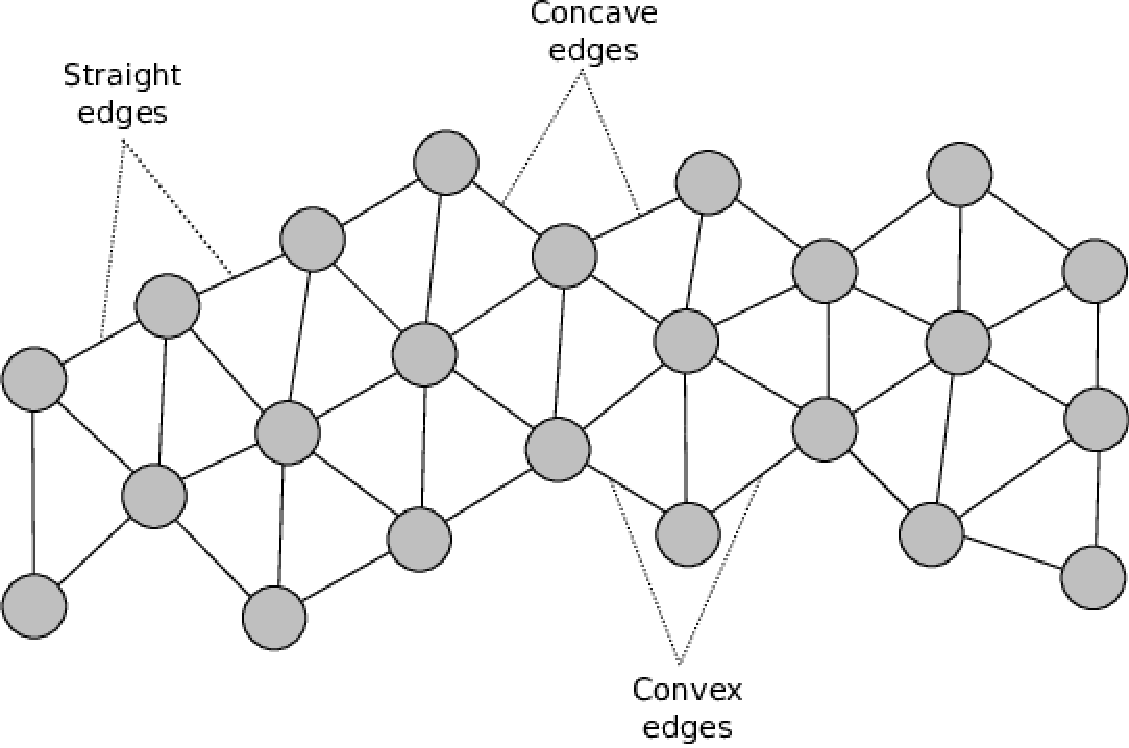
\includegraphics[width=5cm]{figures/SwarmStableShape1}
%% \end{center}
%% \caption{Stable swarm edges\label{concave:SwarmStableShape1}}
%% \end{figure}
The problem with these anomalies is that, although they are stable due to the balancing of the \textit{inter-agent vectors}, they create non-uniform structures that may be unsuitable for tasks that require a uniform swarm formation.

\textit{Concave reduction} is a form of self-healing, it is a process that creates a movement that makes a swarm coalesce towards a more geometrically stable shape. This is achieved by removing voids and concave edges. The techniques defined in this paper function without the need for inter-agent or global messaging using only local proximity detection.

\section{Related Work}\label{sec:RelatedWork}
Research has identified several approaches to resolving swarm structure issues. A prototype framework for self-healing swarms was developed by Dai et al. which considered the problem of agent failure in hostile environments~\cite{DHMRZ:06}. This is in line with work carried out by Vassev and Hinchey who model swarm deployment using ASSL (Autonomic System Specification Language)~\cite{VH:09}. This technique was used by NASA (National Aeronautics and Space Administration) when developing their ANTS (Autonomous Nano Technology Swarm) for use in asteroid belt exploration. This line of research is more focused towards an agent's internal systems failure rather than the removal of anomalies in a swarm distribution. Roach et al. takes a different approach and focuses on the effects of sensor failure and the effect that has on agent distribution~\cite{RMT:15}. The closest research to concave reduction, as discussed in this paper, is that of Lee and Chong who identify the issue of concave edges within swarms in an attempt to create regular lattice formations~\cite{GN:08}. The main focus of their paper is the restructuring of the internal distribution of inter-agent formations. The research by Ismail and Timmis used the approach of \textit{bio-inspired} healing using \textit{granuloma formation}, a biological method for encapsulating an antigen~\cite{IT:10}. They also consider the effects failed agents can have upon a swarm when traversing a terrain \cite{TIBW:16}. 
Concave reduction is an extension of the work discussed by Ismail and Timmis in their papers on `self-healing' \cite{IT:10} and the effects of failed agents \cite{TIBW:16}. It also builds upon Lee and Chong's work on identifying concave edges~\cite{GN:08}. The technique also draws on the work of McLurkin and Demaine who have developed algorithms to detect perimeter types~\cite{MD:09}. The technique employed in this paper does not require the identification of the perimeter type as this would require a communications infrastructure.

\section{Swarm Model}\label{sec:Swarm Model}
To describe the removal of voids a swarming model needs to be defined.

\Figure[t!](topskip=0pt, botskip=0pt ){figures/neighbours} {Neighbour agents\label{define:neighbours}}

An agent $b$ in the swarm ($b\in\mathcal S$) has a sensor ($S_b$) that detects other agents
($b'$)in the swarm
determining their range $r$  and direction $\beta$.  From this data the agent generates a
set of neighbours ($\mathcal N_b$) that are within a specific range.  Usually the range of the
cohesion field $C_b$.

The Agent creates a set of neighbours containing range and bearing pairs
$(r,\beta)$ as shown in equation~\ref{set:Nb} and
figure~\ref{define:neighbours}

\begin{equation}
\mathcal N_b = \{ (r,\beta) \ldots \}
\label{set:Nb}
\end{equation}
These range and bearing pairs are the relative position vector for each
neighbour $b'$ with respect to the sensor reference frame of agent $b$.
Alternative notations are given in equation \ref{notation}
\begin{equation}
	\mathcal N_b = \{(r,\beta) \ldots \} = \{ (r_{b'}, \beta_{b'}) \ldots \} = \{
	b' \ldots \}
	\label{notation}
\end{equation}

The model use is the same as that defined by Eliot et. al. in their paper that introduces a new magnitude based metric~\cite{EKB:18}. 
Equation~\ref{eq:BotPhysics1} defines a weighted model that includes cohesion,
repulsion, direction and obstacle avoidance ($v_c(b), v_r(b),
v_d(b), v_o(b)$). 
The weightings $k_c, k_r, k_d, k_o$ allow each component to be scaled to tailor the swarming effect. 

\begin{equation}\label{eq:BotPhysics1}
  v(b) = k_cv_c(b) + k_rv_r(b) + k_dv_d(b) + k_ov_o(b)
\end{equation}

\textit{Repulsion} $v_r(b)$, defined in Equation~\ref{eq:Repulsion1}, is the
directional movement required to prevent agents colliding. $\mathcal R_b$ is
the set of agents that are within an agent's $b$ repulsion range.

\begin{equation}\label{eq:Repulsion1}
v_r(b) = 
\frac{1}{\card{\mathcal R_b}}
\left(
	\mathlarger{\mathlarger{\sum_{b' \in \mathcal R_b}}}
	{\left( 1-\frac{\magn{b'}}{R_b} \right)}
	b'
\right)
\end{equation}

\textit{Cohesion} $v_{c}(b)$, defined in Equation~\ref{eq:FlyToCentre1},
calculates the movement that makes an agent move towards other agents to form
a cohesive structure. $\mathcal C_b$ is the set of agents that are within an agent's ($b$) cohesion range.

\begin{equation}\label{eq:FlyToCentre1}
	v_c(b) =
	\frac{-1}{\card{\mathcal C_b}}\left({\mathlarger{\sum_{b' \in
	\mathcal C_b}}{b'}}\right)
\end{equation}

\textit{Direction} $v_d(b)$, defined in Equation~\ref{eq:Direction},
generates a directional vector for an agent to move towards a destination
defined as $d$.

\begin{equation}
\label{eq:Direction}
v_d(b) = d
\end{equation}

Obstacles, like agents, can be represented as a point. As an agent moves it may enter an obstacle's \textit{repulsion field}. If this occurs then the agent should move away. In this paper agents are modelled with a fixed \textit{obstacle repulsion field} ($O_b$). If an agent enters the field a vector of magnitude $O_b$ is applied. If more than one obstacle is within the field, the applied repulsion vector is the sum of the repulsion vectors~(Figure~\ref{fig:Obstacle1}). The resultant vector is normalised and scaled such that the magnitude is the same as the field distance~$O_b$ as shown in Equation~\ref{eq:Obstacle2}.

\begin{figure}[H]
\begin{center}
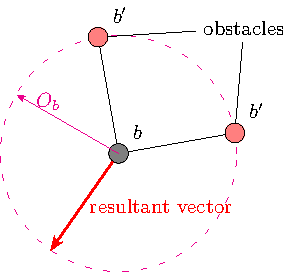
\includegraphics{figures/obstacles}
\end{center}
\caption{Obstacle repulsion \label{fig:Obstacle1}}
\end{figure}

Equation~\ref{eq:Obstacle2} shows the repulsion vector $v_o(b)$ for an agent.
$\mathcal O_b$ is the set of obstacles that are within the range of agent $b$.
The obstacles are identified using the distance between an agent and an
obstacle $o_r$ and comparing the result to the fixed obstacle repulsion
field~$O_b$, so $\forall o \in \mathcal O_b : \magn{o}\leq O_b$.
The applied repulsion is calculated by scaling the normalised sum of the
normalised vectors $\hat o$ by $O_b$.  Note that $\string^$ is the equivalent
of $\hat v = \frac{v}{\magn{v}}$ the normalised vector.

\begin{eqnarray}\label{eq:Obstacle2}
  v_o(b) & = & O_b \hat q_o \\
	\mathrm{where~}  q_o & = & \sum_{o\in \mathcal O_b } \hat o
	\nonumber \\
	v_o(b) & = & O_b \left(\sum_{o\in \mathcal O_b }\hat o\right)^{\!\!\wedge} \nonumber
\end{eqnarray}

An agent's \textit{movement vector} is the sum of all the component vectors as
shown in Equation~\ref{eq:BotPhysics1}. This is a similar technique as used by
Hashimoto et. al.~\cite{HAY:08}. For a vector to be used for movement it be
normalised before the agent's speed ($s_b$)  can be applied. The resultant
\textit{movement vector} $m_b$, as defined in Equation~\ref{eq:AgentMovement}, is calculated using unit time, speed and the normalised \textit{movement vector}.

\begin{equation}\label{eq:AgentMovement}
m_b = s_b  \hat v(b)  t
\end{equation}

Applying the calculations described in this section to all agents in turn creates the swarming effect. 
  
\section{Perimeter Detection}\label{sec:PerimeterDetection}
%In a 2D Euclidean plane a circle provides the maximum area with the minimum perimeter size. A circles perimeter is convex in nature. 
To restructure a disorganised swarm the perimeter agents need to be identified. These agents form part of an outer ({\color{green}green}) or inner edge ({\color{red}red}) (Fig.~\ref{fig:PerimeterBots1}) or are part of an island~(Fig.~\ref{fig:PerimeterBots2}).

The detection mechanism detects both the outer edge of a swarm (equation
\ref{perimeter-predicate})  and any internal features~(voids) that satisfy the same
set of conditions. It is therefore possible to have both voids and islands of
agents within the same swarm~(Fig.~\ref{fig:PerimeterBots2}). Voids are best
defined as perimeters that are concave (equation \ref{concave-predicate}) in nature and inside another perimeter. McLurkin describes two types of perimeters convex and concave~\cite{MD:09}. A convex perimeter is an edge where the average angle of the agent's exposed faces are~$> 180^\circ$. A concave perimeter is where the average exposed angle is~$< 180^\circ$.

\Figure[t!](topskip=0pt, botskip=0pt, midskip=0pt)[width=5cm]{figures/PerimeterBots1}
{Outer Perimeter\label{fig:PerimeterBots1}}

\Figure[t!](topskip=0pt, botskip=0pt, midskip=0pt)[width=8cm]{figures/PerimeterBots2}
{Inner Island Perimeter\label{fig:PerimeterBots2}}
%\subsection{Full-perimeter detection}\label{sec:PerimeterAgentDetection} 


The set of neighbours $\mathcal N_b$ (eqn \ref{set:Nb}) is sorted into a
sequence $\mathcal P_a$ with the bearing values
increasing
\begin{equation}
	\mathcal P_a = \langle (r_0,\beta_0),\ldots,(r_n,\beta_n) \rangle
\end{equation}
such that $\beta_0 < \beta_1 < \ldots < \beta_n$

This set of agents forms the perimeter of an enclosing polygon of agent $b$. 
Each consecutive pair of agents (in the sequence) defines an edge, which has
length $d$ and an angle $\theta$ given by the difference in bearings of
succesive neighbours.  The sequence of edges
that forms this polygon is
\begin{equation}
	\mathcal{P}_e = \langle (d_0,\theta_0), \ldots , (d_n,\theta_n) \rangle
\end{equation}
where
\begin{equation}
	\theta_i = \beta_{i+1} - \beta_i
\end{equation}
the index addition is modulo $|\mathcal N_b|$ making $\beta_0$ the successor
bearing to $\beta_n$ ($n+1 = 0$).  The angles $\theta$ must lie in the range
$0<\theta\leq2\pi$.
This restriction on the values of $\theta$ enforce a condition that
\begin{equation}
	\sum\theta_i = 2\pi
\end{equation}
The length of a perimeter edge is given by the cosine rule
\begin{equation}
	d_i^2 = r_{i+1}^2 + r_i^2 -2r_{i+1}r_i \cos\theta_i
\end{equation}

An agent is on the perimeter of the swarm if it is not enclosed by the polygon
defined in $\mathcal{P}_e$.  Simple geometry shows that this is the case given
by the predicate in equation \ref{enclosing}
\begin{equation}
	\exists \theta_i \in \mathcal{P}_e : \theta_i\geq\pi
	\label{enclosing}
\end{equation}
The polygon is considered `open' if two succesive agents on the perimeter 
cannot see each onther, their separation $d$ is greater that the range of the
attractive field.  An open polygon does not enclose the agent $b$ so it
considered to be on the perimeter.

The agent $b$ is on the perimeter of the swarm if the predicate in equation
\ref{perimeter-predicate} is true.
\begin{equation}
	\exists d_i\in\mathcal{P}_e:d_i>C_b \vee
	\exists\theta_i\in\mathcal{P}_e:\theta_i\geq\pi
	\label{perimeter-predicate}
\end{equation}
An agent is at the apex of a concave region of the perimeter if
\begin{equation}
	\exists(\theta_i,d_i)\in\mathcal{P}_e : d_i>C_b\wedge\theta_i<\pi
	\label{concave-predicate}
\end{equation}


\textit{Orientation independent}  If the agent $b$ is rotated through an angle of $\gamma$ then 
the bearings are rotated by $-\gamma$, \[ \beta_i\mapsto\beta_i-\gamma \]
The  angle between successive agents is now
\[
	\theta_i  =  (\beta_{i+1}-\gamma) - (\beta_i-\gamma)
	 = \beta_{i+1}-\beta_i-\gamma+\gamma
	 = \beta_{i+1}-\beta_i
\]
The predicates are independent of the orientation of the sensing agent.

\section{Concave Reduction Application}\label{sec:ConcaveReductionApplication}
In a static swarm, where there are no \textit{destination vectors}, concave reduction will result in a restructuring motion that creates a more `rounded' swarm as shown in Fig.~\ref{fig:OuterPerimeter3}. Concave reduction also creates a surround effect as it removes voids from a swarm. This is discussed in more detail in section~\ref{voids:ObjectSurrounding}. When concave reduction is applied to a mobile swarm the void closing effect can be used to improve reconnaissance coverage as the swarm passes obstacles. This is discussed in section~\ref{concave:mobileSwarm1}.
Although these effects improve the potential applications of swarms there are negative effects that can be impact introduced. In some circumstances concave reduction can create an artificial \textit{destination vector} in that the swarm will appear to have a directional movement. 

To implement void reduction full perimeter detection is required. The
identification of candidate agents is incorporated into the perimeter
detection algorithm as shown in equation~\ref{concave-predicate}. The addition is to set a status flag to highlight when a gap is detected and to record the agent's that create the gap. Concave reduction does not require the perimeter type to be identified and no communications infrastructure is required. Many coordination algorithms require inter-agent communications~\cite{MD:09,NIM:09,SOM:12,ZFG:13,JG:13}. The disadvantage of requiring a communications infrastructure is that the size of a swarm is limited through message propagation.

\subsection{Perimeter Exceptions}\label{concave:Exceptions}
When a swarm is forming or disrupted through either agent failures, catastrophic events or interactions with obstacles, sections of the swarm may become isolated. When this occurs the sections can be considered to be separate sub-swarms. It is also possible for sections of the swarm to remain connected through tenuous links of either 1 or 2 agents as shown in Figs.~\ref{fig:Connector1} and \ref{fig:Connector2}. In the case of a link connection~(Fig.~\ref{fig:Connector1}) concave reduction can be applied as normal. In the case of a `bridge' link (Fig.~\ref{fig:Connector2}) there is an issue in that there is more than one concave gap. As there is no communications infrastructure in swarm model. One option is allow the swarming algorithm to be applied; this is a reasonable approach as the overall structure of the swarm is unknown therefore the movement cannot be optimised. An alternative approach would be to select either the largest or the smallest gap; again as the structure of the swarm is unknown this may not be beneficial. A third option would be to select one of the gaps (randomly, first seen, last seen) and implement the concave reduction at that point. The approach taken in this paper is to select the first gap that is detected. Selecting the first gap reduces the computational overhead of the algorithm.

\Figure[t!](topskip=0pt, botskip=0pt, midskip=0pt)[width=4cm]{figures/PerimeterBots4}{Link\label{fig:Connector1}}
%% \begin{figure}
%% \begin{center}
%% 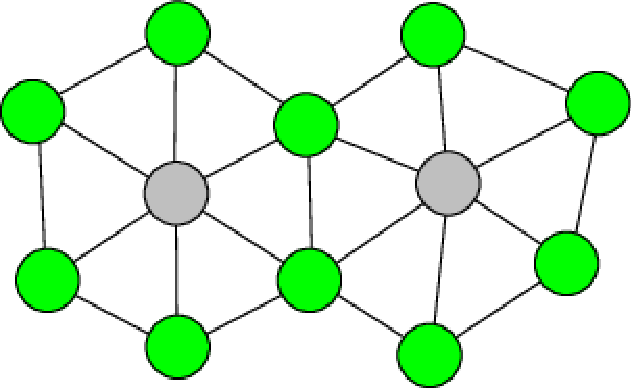
\includegraphics[width=4cm]{figures/PerimeterBots4}
%% \end{center}
%% \caption{Link\label{fig:Connector1}}
%% \end{figure}
\Figure[t!](topskip=0pt, botskip=0pt, midskip=0pt)[width=5cm]{figures/PerimeterBots5}{Bridge\label{fig:Connector2}}
%% \begin{figure}
%% \begin{center}
%% 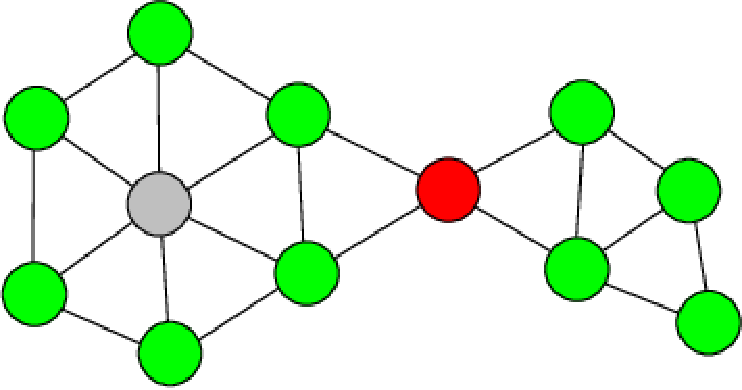
\includegraphics[width=4cm]{figures/PerimeterBots5}
%% \end{center}
%% \caption{Bridge\label{fig:Connector2}}
%% \end{figure}

\section{Concave reduction agent movement}\label{concave:AgentMovement}
Adding a further characteristic to the motion of a swarm necessitates a revision to the existing agent model~(Equation.~\ref{eq:BotPhysics1}). With concave reduction this revision is based upon the identification of the concave perimeter edges as shown in~Fig.~\ref{concave:VoidConcave1} as $(b^{'},b,b^{''})$. 
% \begin{figure}
% \begin{center}
% \includegraphics[width=5cm]{figures/VoidConcave1}
% \end{center}
% \caption{Agent concave motion\label{concave:VoidConcave1}}
% \end{figure}

\Figure[t!](topskip=0pt, botskip=0pt, midskip=0pt)[width=5cm]{figures/VoidConcave1}{Agent concave motion\label{concave:VoidConcave1}}

When an agent is identified as being a component of a concave
characteristic~(eqn.~\ref{concave-predicate}) the normal \textit{movement-direction vector} is replaced by a \textit{concave reduction vector}. This new vector causes the agent to move in a direction that will reduce or remove a concave edge by moving the agent towards the identified gap. The effect of this will be to either straighten an outer perimeter or reduce/remove a void. This change in direction effects the distance and magnitude variances due to the changes induced. Figures~\ref{fig:InterAgentEffect1} and \ref{fig:InterAgentEffect2} shows this effect in more detail. Figure~\ref{fig:InterAgentEffect1}~shows the initial positions of the agents before the concave reduction is applied to the agent. Figure~\ref{fig:InterAgentEffect2}~shows the effects on the relationship with the agent's neighbours. The aggregate change is an increase in the inter-agent distances and an increase in the resultant magnitude effects.

\Figure[t!](topskip=0pt, botskip=0pt, midskip=0pt)[width=5cm]{figures/InterAgentEffect1}{Initial Position\label{fig:InterAgentEffect1}}
%% \begin{figure}
%% \begin{center}
%% \includegraphics[width=5cm]{figures/InterAgentEffect1}
%% \end{center}
%% \caption{Initial Position\label{fig:InterAgentEffect1}}
%% \end{figure}

\Figure[t!](topskip=0pt, botskip=0pt, midskip=0pt)[width=5cm]{figures/InterAgentEffect2}{Reduced Position\label{fig:InterAgentEffect2}}
%% \begin{figure}
%% \begin{center}
%% 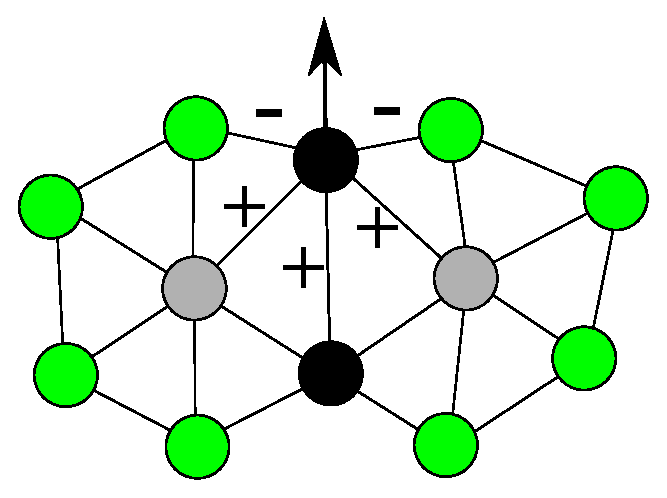
\includegraphics[width=5cm]{figures/InterAgentEffect2}
%% \end{center}
%% \caption{Reduced Position\label{fig:InterAgentEffect2}}
%% \end{figure}

\section{Concave Reduction Perimeter Effect}\label{sec:ConcaveReductionPerimeterEffect}
A swarm's perimeter can be used to modify its behaviour, such as reducing sensor requirements by reducing the need for GPS sensors or coordinating a swarm to a destination. Generally when discussing agent angles in relation to a perimeter it refers to the average angle or all the agents on a boundary i.e. to detect inner or outer perimeters. When discussing \textit{concave reduction} the angle of interest is the relationship between an agent and two of its adjacent neighbours such that the neighbours have no visibility of each other and the \textit{neighbour-agent-neighbour} relationship produces an angle~$< 180^\circ$. Concave reduction affects both inner~(Fig.~\ref{fig:InnerPerimeter1}) and outer~(Fig.~\ref{fig:OuterPerimeter1}) perimeter agents. Figures~\ref{fig:OuterPerimeter1} and \ref{fig:InnerPerimeter1} show candidate agents, in black, identified by this process. 

\Figure[t!](topskip=0pt, botskip=0pt, midskip=0pt)[width=4cm]{figures/OuterPerimeter1}{Outer Perimeter\label{fig:OuterPerimeter1}}
%% \begin{figure}
%% \begin{center}
%% 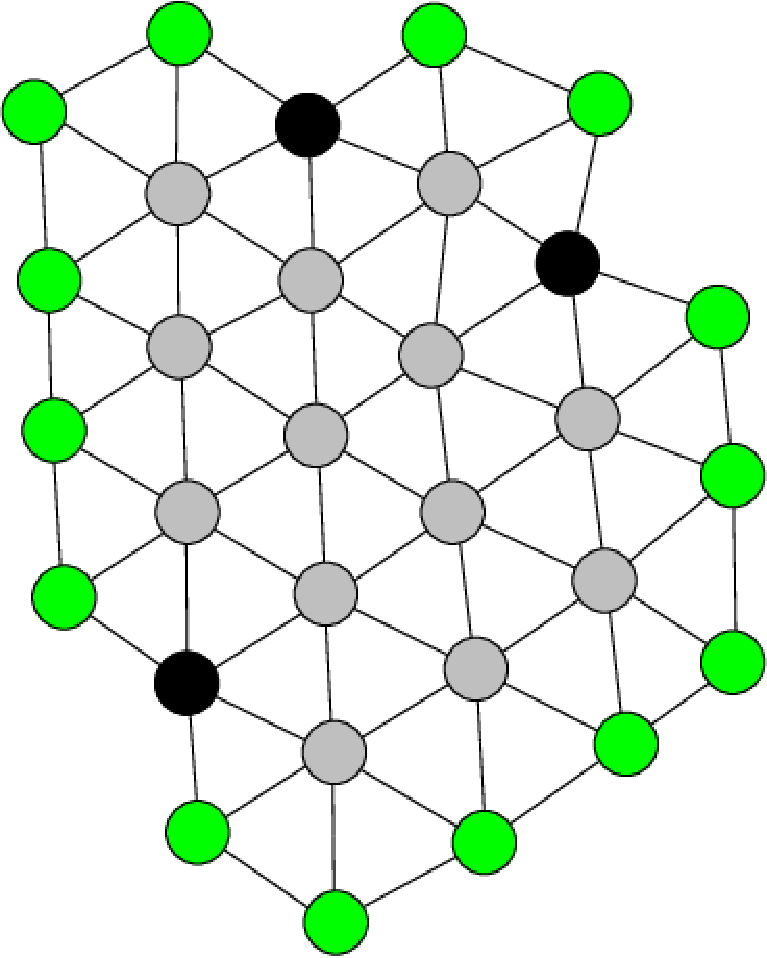
\includegraphics[width=4cm]{figures/OuterPerimeter1}
%% \end{center}
%% \caption{Outer Perimeter\label{fig:OuterPerimeter1}}
%% \end{figure}

\Figure[t!](topskip=0pt, botskip=0pt, midskip=0pt)[width=4cm]{figures/InnerPerimeter1}{Inner Perimeter\label{fig:InnerPerimeter1}}
%% \begin{figure}
%% \begin{center}
%% 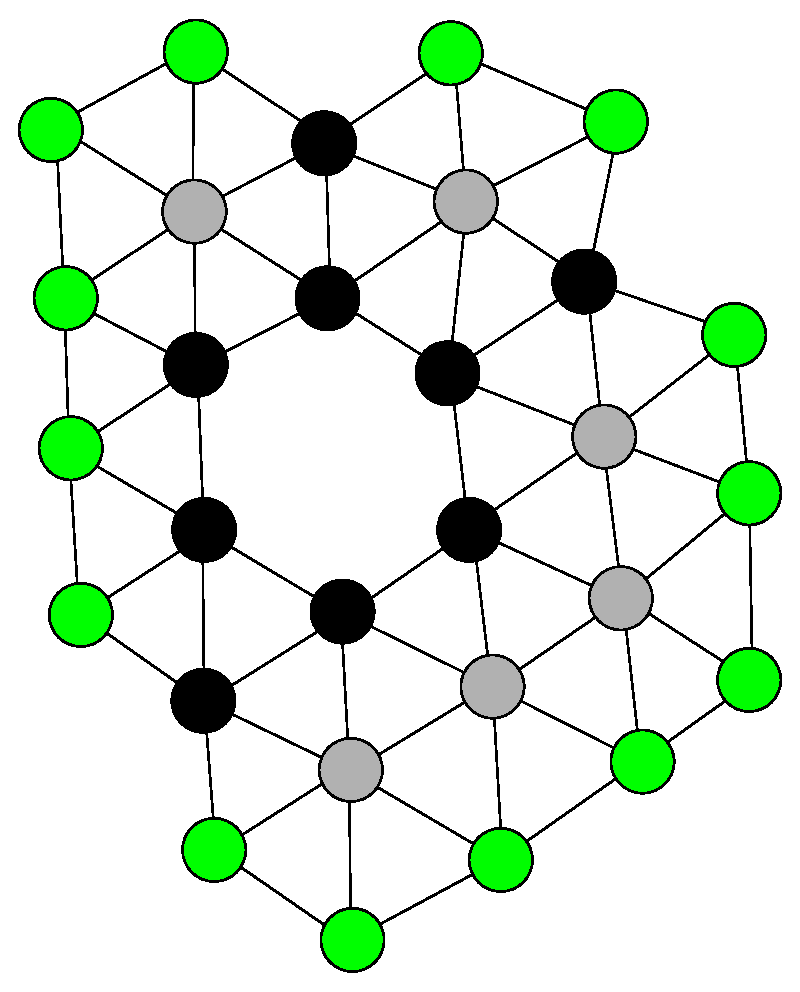
\includegraphics[width=4cm]{figures/InnerPerimeter1}
%% \end{center}
%% \caption{Inner Perimeter\label{fig:InnerPerimeter1}}
%% \end{figure}

The purpose of \textit{concave reduction} is to alter the overall structure of the swarm by replacing the calculated \textit{movement-direction vector} on anomalous perimeter agents. These perimeter based changes cause a cascading movement within the swarm as a non-perimeter based agent's attempt to move towards a position of equilibrium with respect to its neighbours. The movement on a concave perimeter~(internal void) creates a movement that closes a void by \textit{percolating} it out of the swarm~(Figs.~\ref{fig:InnerPerimeter2}~and~\ref{fig:InnerPerimeter3}). The movement on the convex perimeter's (outer perimeter) deformities (indents) creates a convex or straight edge as shown in Figs.~\ref{fig:OuterPerimeter2}~and~\ref{fig:OuterPerimeter3}.

\Figure[t!](topskip=0pt, botskip=0pt, midskip=0pt)[width=4cm]{figures/PerimeterBotsCircle3}
{Concave reduction effect on perimeters\label{fig:InnerPerimeter2}}
%% \begin{figure}
%% \begin{center}
%% 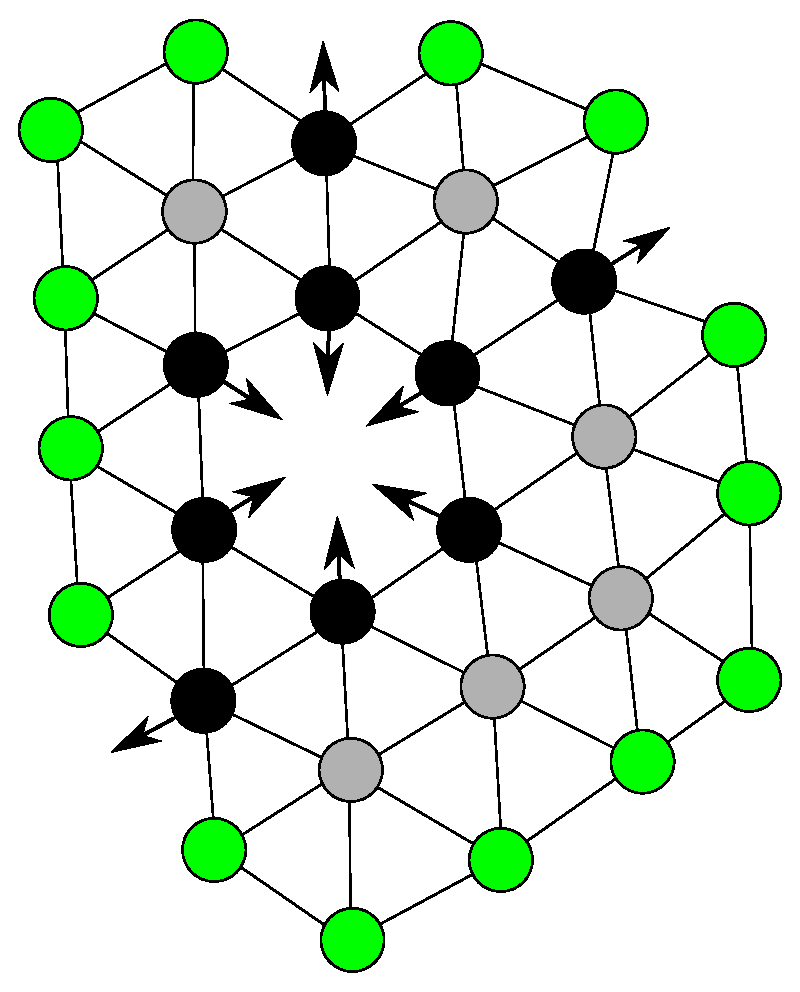
\includegraphics[width=4cm]{figures/PerimeterBotsCircle3}
%% \end{center}
%% \caption{Inner Perimeter\label{fig:InnerPerimeter2}}
%% \end{figure}
\Figure[t!](topskip=0pt, botskip=0pt, midskip=0pt)[width=4cm]{figures/PerimeterBotsCircle4}{Concave reduction result\label{fig:InnerPerimeter3}}
%% \begin{figure}
%% \begin{center}
%% \includegraphics[width=4cm]{figures/PerimeterBotsCircle4}
%% \end{center}
%% \caption{Void reduction result\label{fig:InnerPerimeter3}}
%% \end{figure}
\Figure[t!](topskip=0pt, botskip=0pt, midskip=0pt)[width=4cm]{figures/PerimeterBotsCircle1}{Outer Perimeter (swarm without voids)\label{fig:OuterPerimeter2}}
%% \begin{figure}
%% \begin{center}
%% 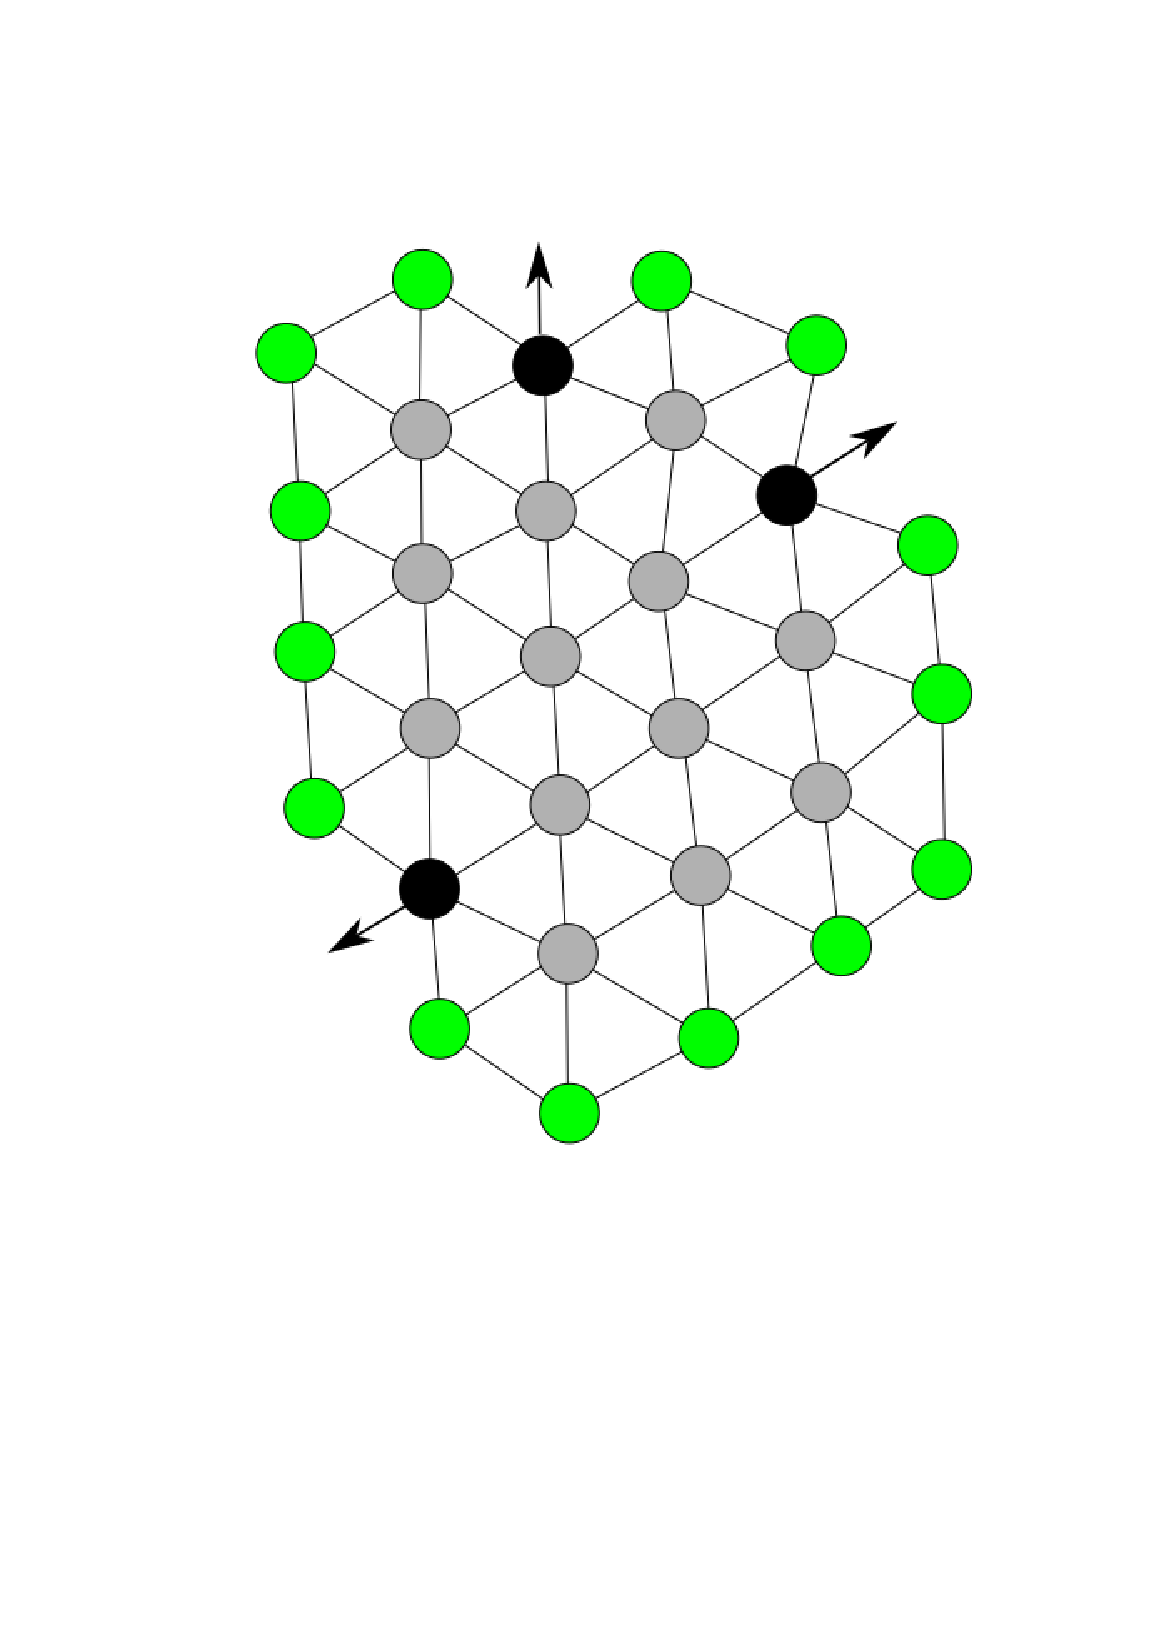
\includegraphics[width=4cm]{figures/PerimeterBotsCircle1}
%% \end{center}
%% \caption{Outer Perimeter\label{fig:OuterPerimeter2}}
%% \end{figure}
\Figure[t!](topskip=0pt, botskip=0pt, midskip=0pt)[width=4cm]{figures/PerimeterBotsCircle2}{Concave reduction result (swarm without voids)\label{fig:OuterPerimeter3}}
%% \begin{figure}
%% \begin{center}
%% 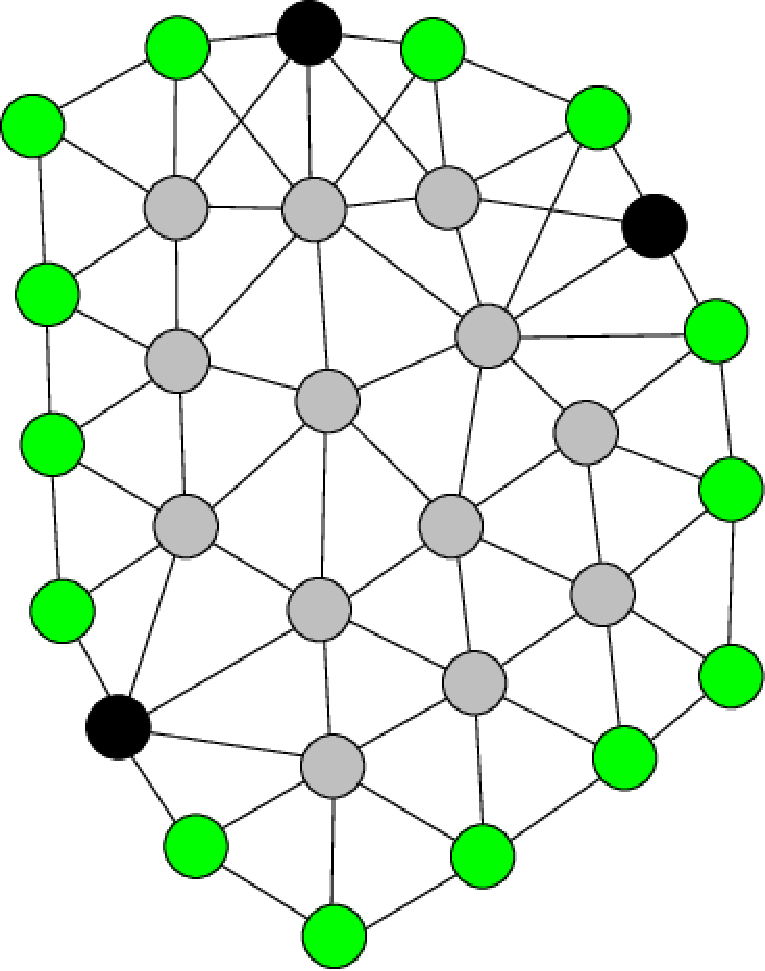
\includegraphics[width=4cm]{figures/PerimeterBotsCircle2}
%% \end{center}
%% \caption{Void reduction result\label{fig:OuterPerimeter3}}
%% \end{figure}

\section{Concave reduction mathematical model}\label{concave:ConcaveVoidReduction1}
% As part of identifying a perimeter each agent's neighbours must be sorted by angle. A pair of agents are identified as a set $b.gap$ ($b.gap \equiv G_b$). 
When an agent is on the perimeter, equation \ref{concave-predicate} is
satisifed, it is subject to concave reduction.
The pair of neighbours that form the concave element is $\mathcal G_b$, the
gap in the perimeter.
Equation~\ref{eq:ConcaveVoidPhysics3} calculates the centroid of the gap agents. 

% Equation~\ref{eq:ConcaveVoidPhysics1} generates the dictionary set of all the neighbours along with an angle that each of the agent's neighbours make with the first detected neighbour. $nbr(b)$ returns a set consisting of an agent's ($b$) neighbours.

%\begin{equation}
%\label{eq:ConcaveVoidPhysics1}
%S_b \buildrel \Delta \over = \{(b',\angle(b'~b~b^0)) : b' \in nbr(b)\}
%\end{equation}

The mid-point $D(b)$ is then calculated as below in Equation~\ref{eq:ConcaveVoidPhysics3}.

\begin{equation}
\label{eq:ConcaveVoidPhysics3}
D(b) = \frac{1}{2}\sum_{b' \in \mathcal G_b}b' 
\end{equation}

$D(b)$~is the \textit{concave reduction} vector is derived from the identified
mid-point of the neighbour gap~($\mathcal{G}_b$) to the parent agent~($b$) as
shown in Equation~\ref{eq:ConcaveVoidPhysics3}.

The final vector needs to accommodate an agent's surroundings. Due to agent
proximity it can be assumed that there are no agents in the path between the
agent and the gap, however, there may be an obstacle in the agent's path. The
\textit{concave-reduction-vector} must include an obstacle avoidance
component~$v_o(b)$.  As with all the previous vector based calculations a 
weighting is applied $k_{cr}$ to allow the model to vary the intensity of the effects.  
The resultant vector $V(b)$ as shown
in~Equation~\ref{eq:ConcaveVoidPhysics4}  is normalised to produce the \textit{unit-movement-vector}
$\hat V(b)$.

\begin{equation}\label{eq:ConcaveVoidPhysics4}
V(b) = (k_{cr}D(b) + k_ov_o(b))
\end{equation}

\section{Swarm Metrics}

\subsection{Distance Metric}

Equation~\ref{eq:SwarmStabilityDistance1} calculates the mean distance of an
agent to its neighbours $\mathcal{N}_b$. 
%% The relative position vector generated for an agent $b$ to its neighbour $b'$, $bb'$, is shown in~(\ref{eq:FlyToCentre1}). The magnitude of that vector gives the distance between two agents. For an individual agent the average magnitude $\mu_d(b)$ is calculated as \ref{eq:SwarmStabilityDistance1} where $b$ is the agent and $|nbr(b)|$ is the number of neighbours.

\begin{equation}
\label{eq:SwarmStabilityDistance1}
\mu_d(b) =
\frac{1}{\mathlarger{\card{\mathcal{N}_b}}}\left({\mathlarger{\sum_{b' \in
\mathcal{N}_b}}\magn{b'}}\right)
\end{equation}

The mean distance for a swarm is calculated
by~Equation~\ref{eq:SwarmStabilityDistance2}. All the inter-agent distances
are included for the swarm ($\mathcal S$). 

%% $\sum_{b \in S}|nbr(b)|$ calculates how many inter-agent relationships exist in the swarm and $\sum_{b' \in nbr(b)}|bb'|$ calculates the total distance between each agent and its neighbours. $\sum_{b \in S}$ iterates over all the agents in the swarm~($S$).

\begin{equation}
\label{eq:SwarmStabilityDistance2}
\mu_d(\mathcal S) = \frac{\mathlarger{\sum_{b \in
\mathcal S}}~\mathlarger{\sum_{b' \in
\mathcal{N}_b}}\magn{b'}}{\mathlarger{\sum_{b \in
\mathcal S}\card{\mathcal{N}_b}}}
\end{equation}

%\section{Standard deviation in distance metric}\label{Section:VarianceInDistance}
The mean distance provides a indication of the large scale structure of the swarm. However it is not sufficient to give an indication of the internal distribution of the agents. The standard deviation clarifies the distribution within the swarm as shown in~Equation~\ref{eq:SwarmStabilityDistance3}. 

%% $(|bb'| - \mu(S))^2$ is the square of the difference in a distance to the mean and $\sum_{b \in S}~\sum_{b' \in nbr(b)}$ calculates the number of inter-agent interactions.

\begin{equation}
\label{eq:SwarmStabilityDistance3}
\sigma_d(\mathcal S) = \sqrt{\frac{\mathlarger{\sum_{b \in
\mathcal S}}~\mathlarger{\sum_{b' \in \mathcal{N}_b}}\Big(\magn{b'} -
\mu_d(\mathcal S)\Big)^2}{\mathlarger{\sum_{b \in
\mathcal S}\card{\mathcal{N}_b}}}}
\end{equation}

The distance-based metric for the internal distribution of the agents is therefore $\mu_d(\mathcal S)$ and $\sigma_d(\mathcal S)$. This can be written informally as:

\begin{equation}
\label{eq:SwarmDistanceMetric}
\psi_d(\mathcal S) = \mu_d(\mathcal S)\pm \sigma_d(\mathcal S)
\end{equation}

\subsection{Magnitude Metric}

The metric used to analyse the swarm changes are defined by Eliot et. al. in~\cite{EKB:18}. Each agent $b$ can be analysed based upon a \textit{cohesion/repulsion scalar}, $P(b)$, to measure the influence of the neighbours of $b$ as cohesive (positive) or repulsive (negative) as shown in Equation~\ref{eq:CohesionRepulsion}.

\begin{equation}
\label{eq:CohesionRepulsion}
P(b) = \left\{\begin{array}{lll}
               |v(b)|& \mathrm{if} & |k_c v_c(b)| > |k_r v_r(b)|\\
              -|v(b)|& \mathrm{otherwise}
              \end{array}\right.
\end{equation}

Although it is possible for $v(b)$ to be null there could still be variation in the constituent components. The variation calculation (standard deviation) as shown in Equation~\ref{eq:SwarmStabilityQuotientT}. 

The mean cohesion/repulsion scalar for the swarm is now given by~(\ref{eq:SwarmStabilityMetricT3}).  

\begin{equation}
\label{eq:SwarmStabilityMetricT3}
\mu_p(\mathcal S) = \frac{\mathlarger{\sum_{b \in \mathcal S} P(b)}}{\mathlarger{\sum_{b \in \mathcal S}}|\mathcal{N}_b| + \mathlarger{\sum_{b \in \mathcal S}}|\mathcal R_b|}
\end{equation}
Where $\mathcal R_b$ is the set of neighbours subject to repulsion, 
where $\mathcal R_b \subseteq \mathcal N_b$ and $b'\in\mathcal R_b:\magn{b'}\leq R_b$
The standard deviation associated with this mean is calculated as Equation~\ref{eq:SwarmStabilityQuotientT}.

\begin{equation}
\label{eq:SwarmStabilityQuotientT}
\sigma_p(\mathcal S) = \sqrt{\frac{\mathlarger{\sum_{b \in \mathcal S}}\Big(P(b)-\mu_p(\mathcal S)\Big)^2}{\mathlarger{\sum_{b \in \mathcal S}}|\mathcal{N}_b| + \mathlarger{\sum_{b \in \mathcal S}}|\mathcal R_b|}}
\end{equation}

The metric for the internal movement is this pair of numbers, the mean and standard deviation of the swarm's internal \textit{cohesion/repulsion}. The pair $\mu_p(\mathcal S)$, $\sigma_p(\mathcal S)$ may be written informally as: 

\begin{equation}
\label{eq:SwarmPotentialMagnitude}
\psi_p(\mathcal S) = \mu_p(\mathcal S)\pm \sigma_p(\mathcal S)
\end{equation}

\section{Effect of concave reduction on swarm structure}
If there is a `gap' on a perimeter then the \textit{concave-reduction-vector} is applied instead of the normal \textit{interaction-vector}. To test this effect a baseline is established for a comparison.

The comparison takes into consideration not just the jitter identified by the distance and magnitude metrics but also the effect on the number of identifiable perimeter agents. One of the effects of concave reduction on an unstructured swarm is to reduce the size of the perimeter. Table \ref{tab:BaselineConcaveReduction} shows the simulation parameters for both the baseline and the concave reduction experiments. Figure~\ref{fig:ConcaveInitial} shows the initial deployment of the swarm used for both the baseline and the concave reduction evaluation.

\begin{table}
\caption{Baseline comparison for concave reduction}\label{tab:BaselineConcaveReduction}
\begin{center}
\begin{tabular}{| p{1.4cm} | p{1.2cm} | p{1.2cm} | p{2.5cm} |}
\hline
\bf Weight \bf component & \bf Baseline \bf swarm & \bf Concave \bf reduction & \bf Description \\ \hline
Sample rate & 100 & 100 & ms - Unit sampling interval\\  \hline
$k_{cr}$ & 0 & 100 & weight adjuster for concave reduction vector\\  \hline
$k_c$ & 5 & 5 & weight adjuster for cohesion field\\  \hline
$k_r$ & 15 & 15 & weight adjuster for repulsion field\\  \hline
$k_d$ & 0 & 0 & weight adjuster for destination vector 0 for static baseline 100 from directional\\  \hline
Repulsion Boundary & 70 & 70 & units\\  \hline
Neighbour Distance & 80 & 80 & units\\  \hline
Speed & 20 & 20 & units/s\\  \hline
\end{tabular}
\end{center}
\end{table}

%COVERBASELINESTART.py
\Figure[t!](topskip=0pt, botskip=0pt, midskip=0pt)[width=8.3cm]{figures/ConcaveInitial}{Initial Swarm Deployment\label{fig:ConcaveInitial}}

Figure~\ref{concave:BaselineConcaveEffectDist} shows the changes in the inter-agent distances that result from the concave reduction. The experiment demonstrates that with concave reduction the average distance increases and the variance of the distances increases. This is due to the `pulling' effect of the \textit{concave reduction vector} on the perimeter. The algorithm distorts the distribution of the agents as discussed in section~\ref{concave:AgentMovement}. The initial expansion of the swarm is similar for the baseline and the concave reduction however at 9 seconds into the simulation the \textit{concave reduction vectors} affects the swarm sufficiently to prevent the average distance reducing to the same level as the baseline. Once the swarm has stabilised with the concave reduction enabled the average distance and variance remain constant but above the baseline.
%BASELINE-CONCAVE-DIST.py

\Figure[t!](topskip=0pt, botskip=0pt, midskip=0pt)[width=8.3cm]{figures/BaselineConcaveEffectDist}{Baseline/Concave effect using distance metric\label{concave:BaselineConcaveEffectDist}}
%% \begin{figure}
%% \begin{center}
%% 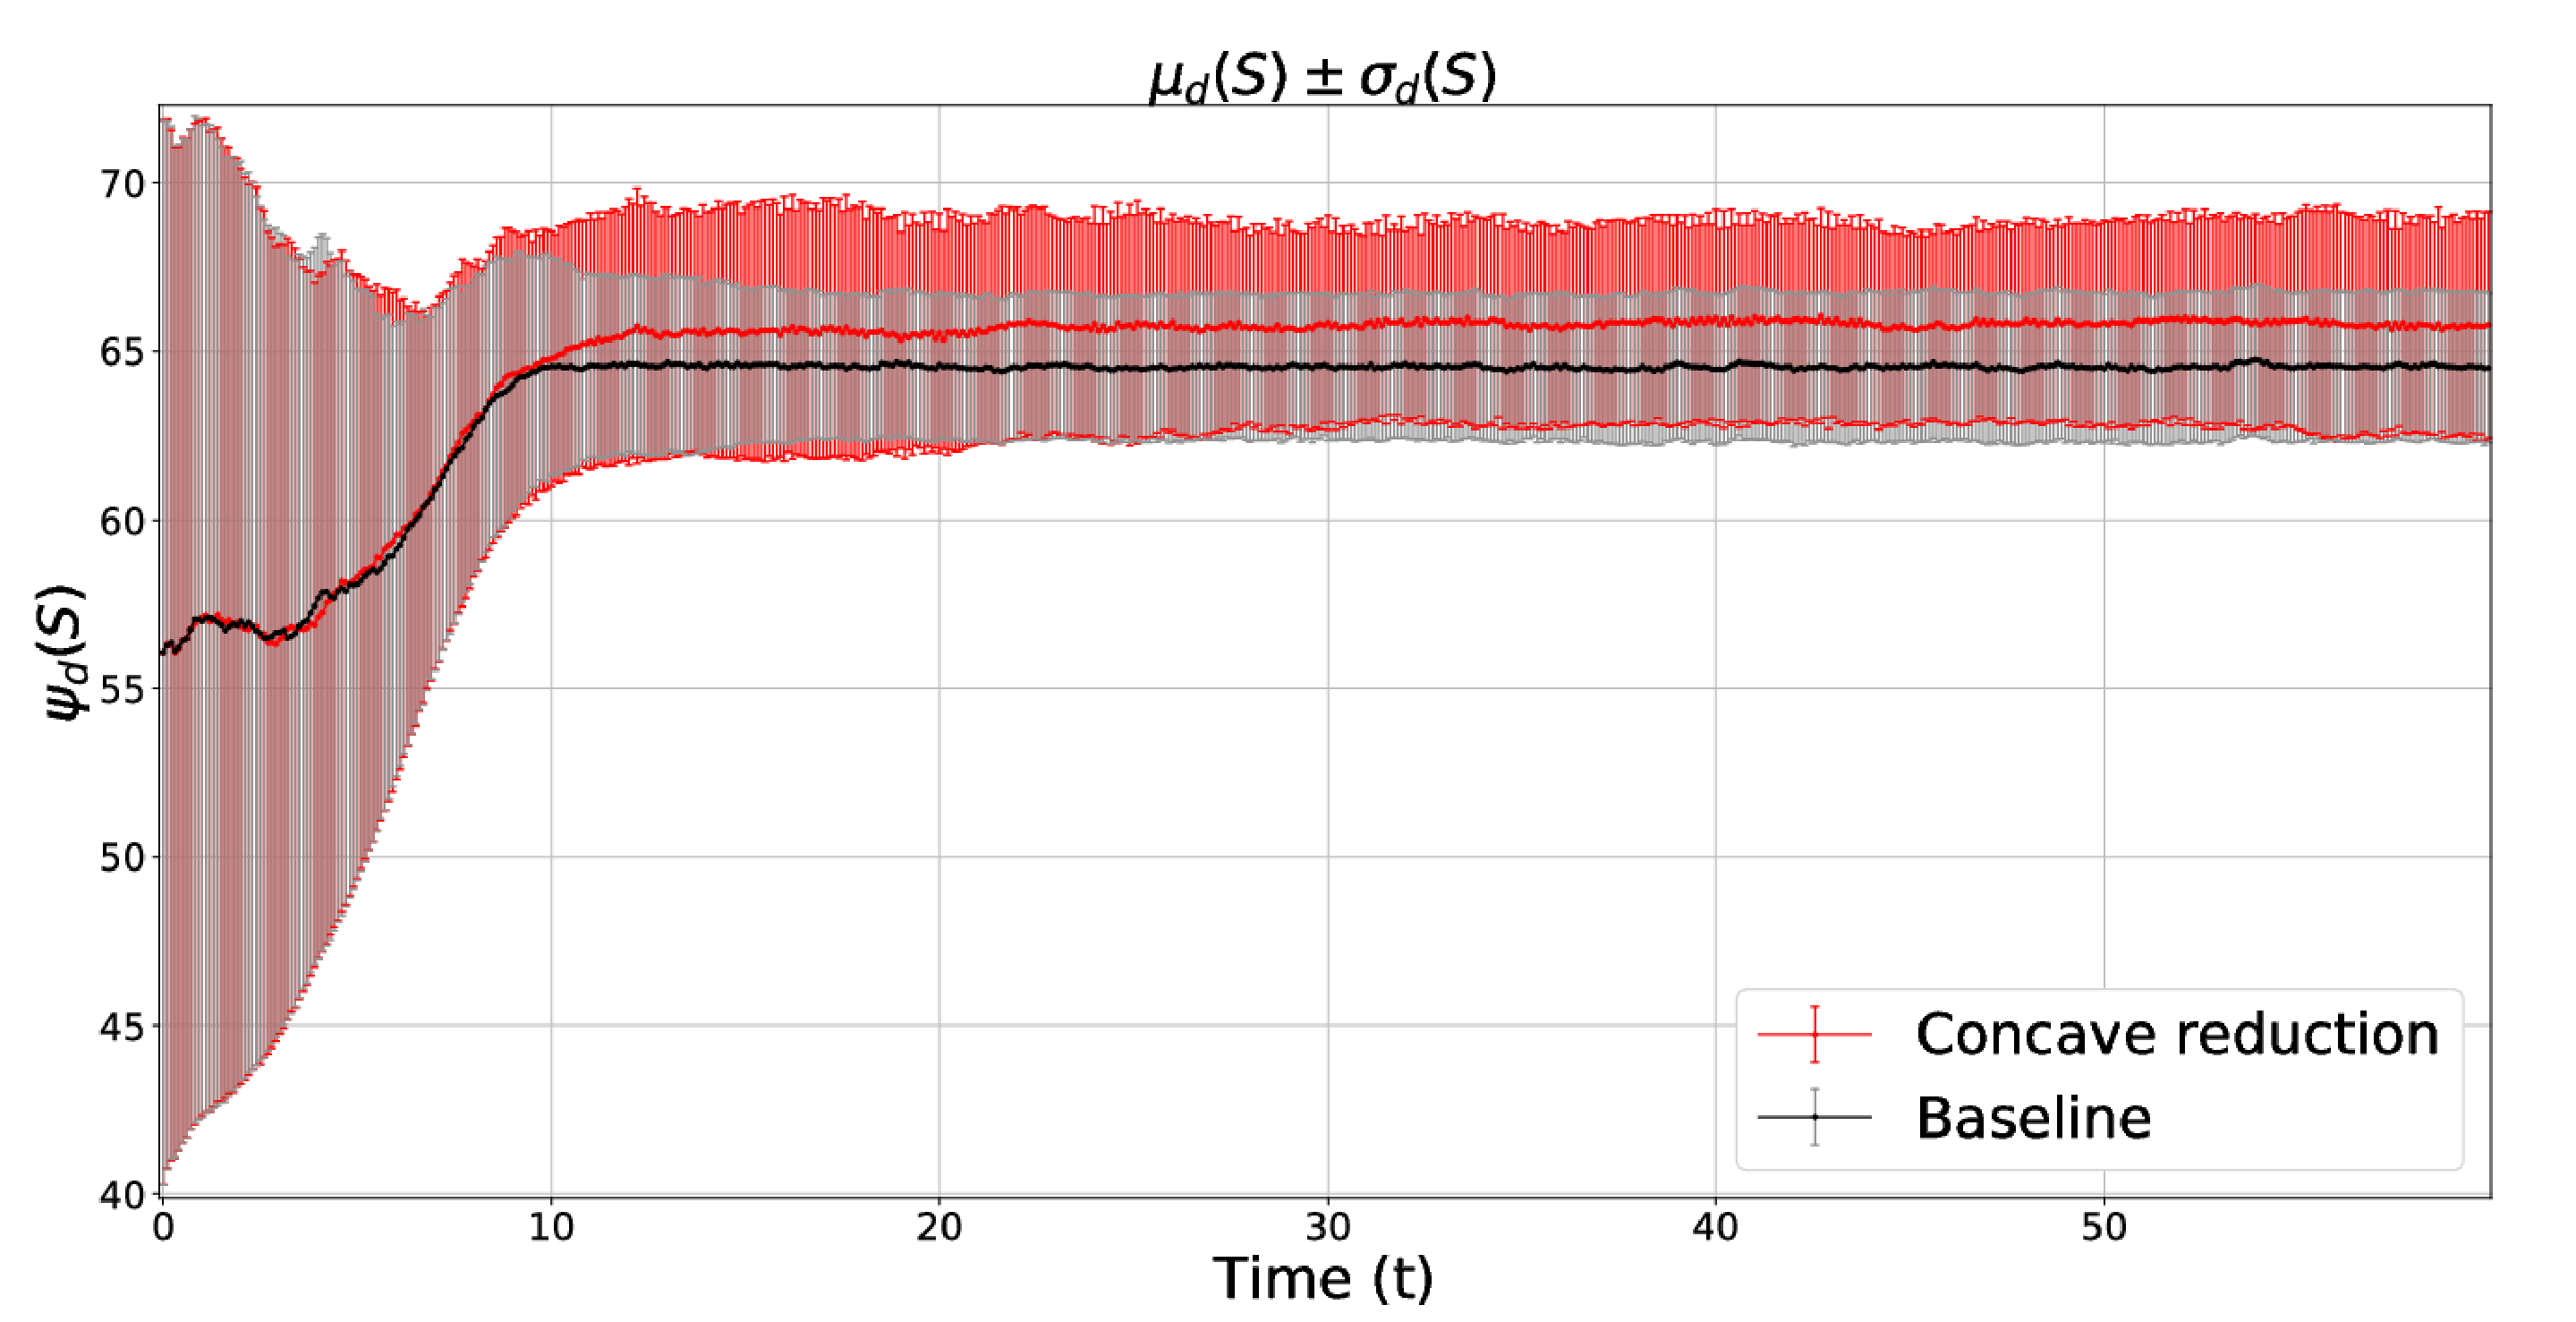
\includegraphics[width=8cm]{figures/BaselineConcaveEffectDist}
%% \end{center}
%% \caption{Baseline/Concave effect distance \label{concave:BaselineConcaveEffectDist}}
%% \end{figure}

Figure~\ref{concave:BaselineConcaveEffectMag} shows the change in the \textit{inter-agent vector magnitudes} that the concave reduction introduces. Both the average magnitude increases and the variance. The magnitude increases as the \textit{concave reduction vector} has caused the agents to move outwards increasing the area of the swarm. The increase in cohesion is a direct result of the increased distance. The field effects still intersect but due to the average distance of the agents being further apart the repulsion is reduced. The agents being further apart causes the increase in cohesion as the algorithm attempts to prevents the swarm from breaking up. The variance increase is caused by the concave reduction effect moving selected agents into less optimal positions.
The \textit{inter-agent vector magnitude} calculations in these experiments are based on the positions of the agents and the cohesion and repulsion field effects. The \textit{concave reduction vector} is not part of the metric calculation. The \textit{concave reduction vector} is only applied to an agent for movement calculation. 
%BASELINE-CONCAVE-MAG.py

\Figure[t!](topskip=0pt, botskip=0pt, midskip=0pt)[width=8.3cm]{figures/BaselineConcaveEffectMag}{Baseline/Concave effect using cohesion/repulsion\label{concave:BaselineConcaveEffectMag}}
%% \begin{figure}
%% \begin{center}
%% 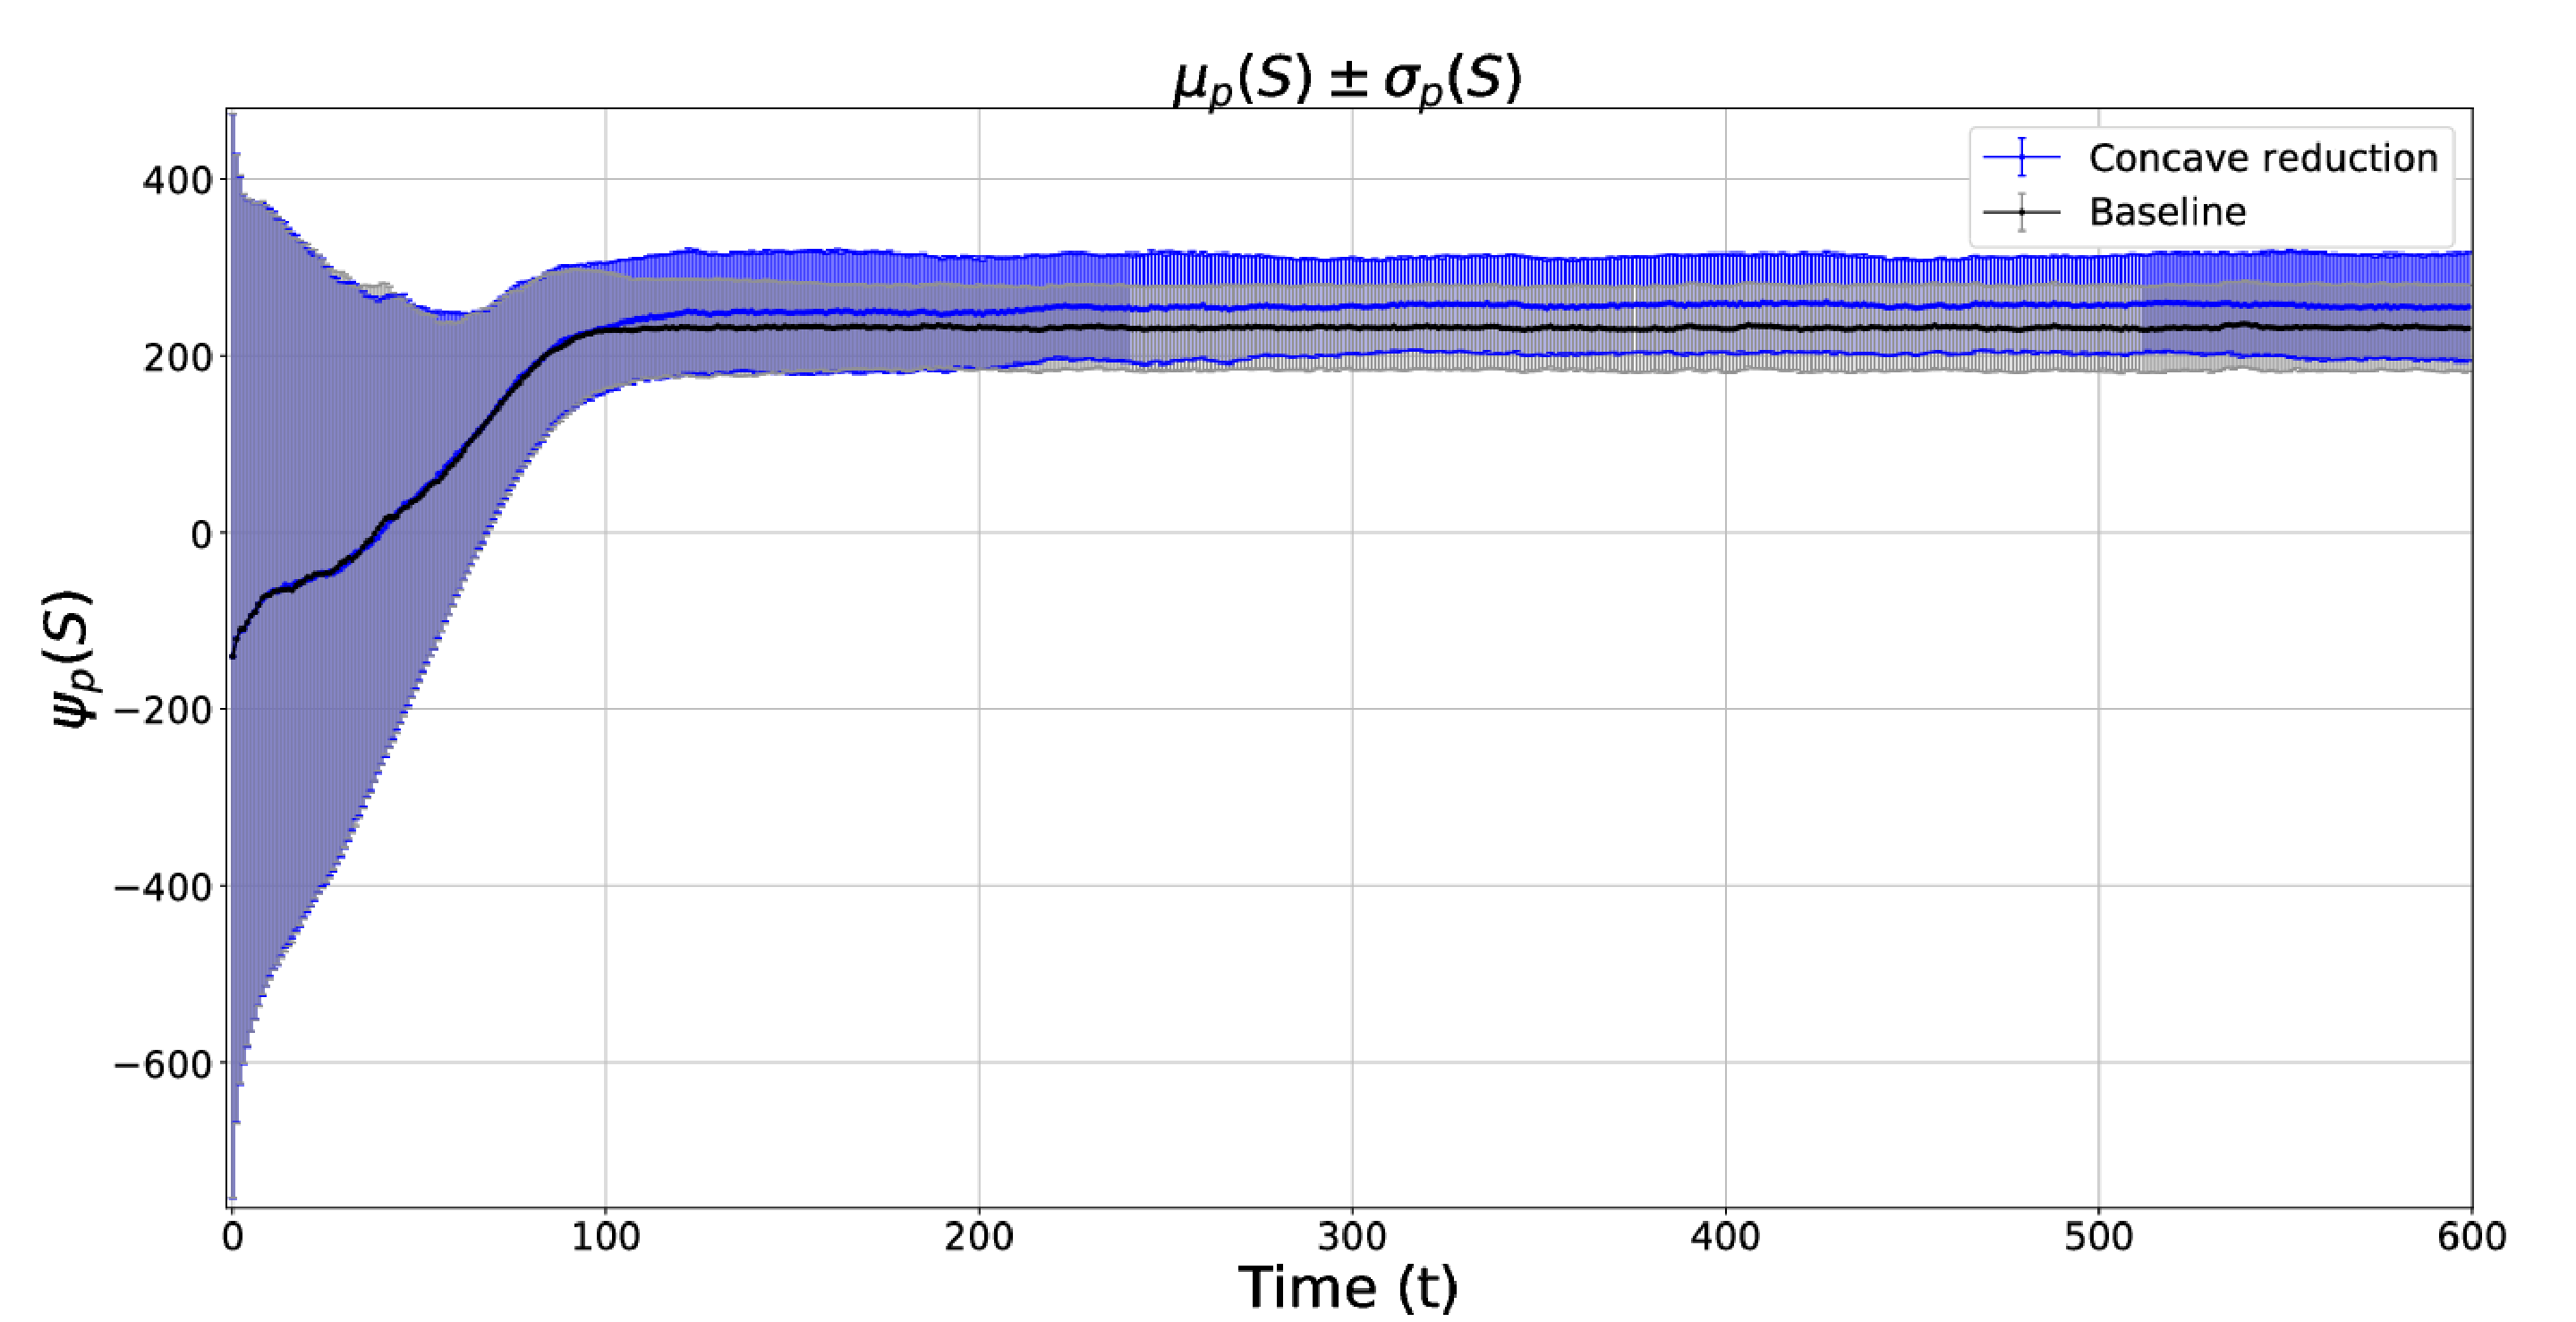
\includegraphics[width=8cm]{figures/BaselineConcaveEffectMag}
%% \end{center}
%% \caption{Baseline/Concave effect magnitude\label{concave:BaselineConcaveEffectMag}}
%% \end{figure}

Figure~\ref{concave:BaselineConcavePerimeter} shows the effect on the number of perimeter agents. Initially the perimeter size is minimally affected due to the swarms compression however after the expansion phase of the swarm (8 seconds) more perimeter agents are identified as concave edges are formed. As these concave edges are `straightened' they create further anomalies that ripple through the swarm. This rippling is identified by the erratic changes in the number of perimeter agents. After approximately 30 seconds the swarm has been forced into a less angular structure with curved edges and the number of perimeter agents falls below the minimum of the baseline. The shape of the swarm is still undergoing change following this and the perimeter count continues to fluctuate.
%PERIMETER8070CONCAVE.py
\Figure[t!](topskip=0pt, botskip=0pt, midskip=0pt)[width=8.3cm]{figures/BaselineConcavePerimeter}{Baseline/Concave perimeter size\label{concave:BaselineConcavePerimeter}}
%% \begin{figure}
%% \begin{center}
%% 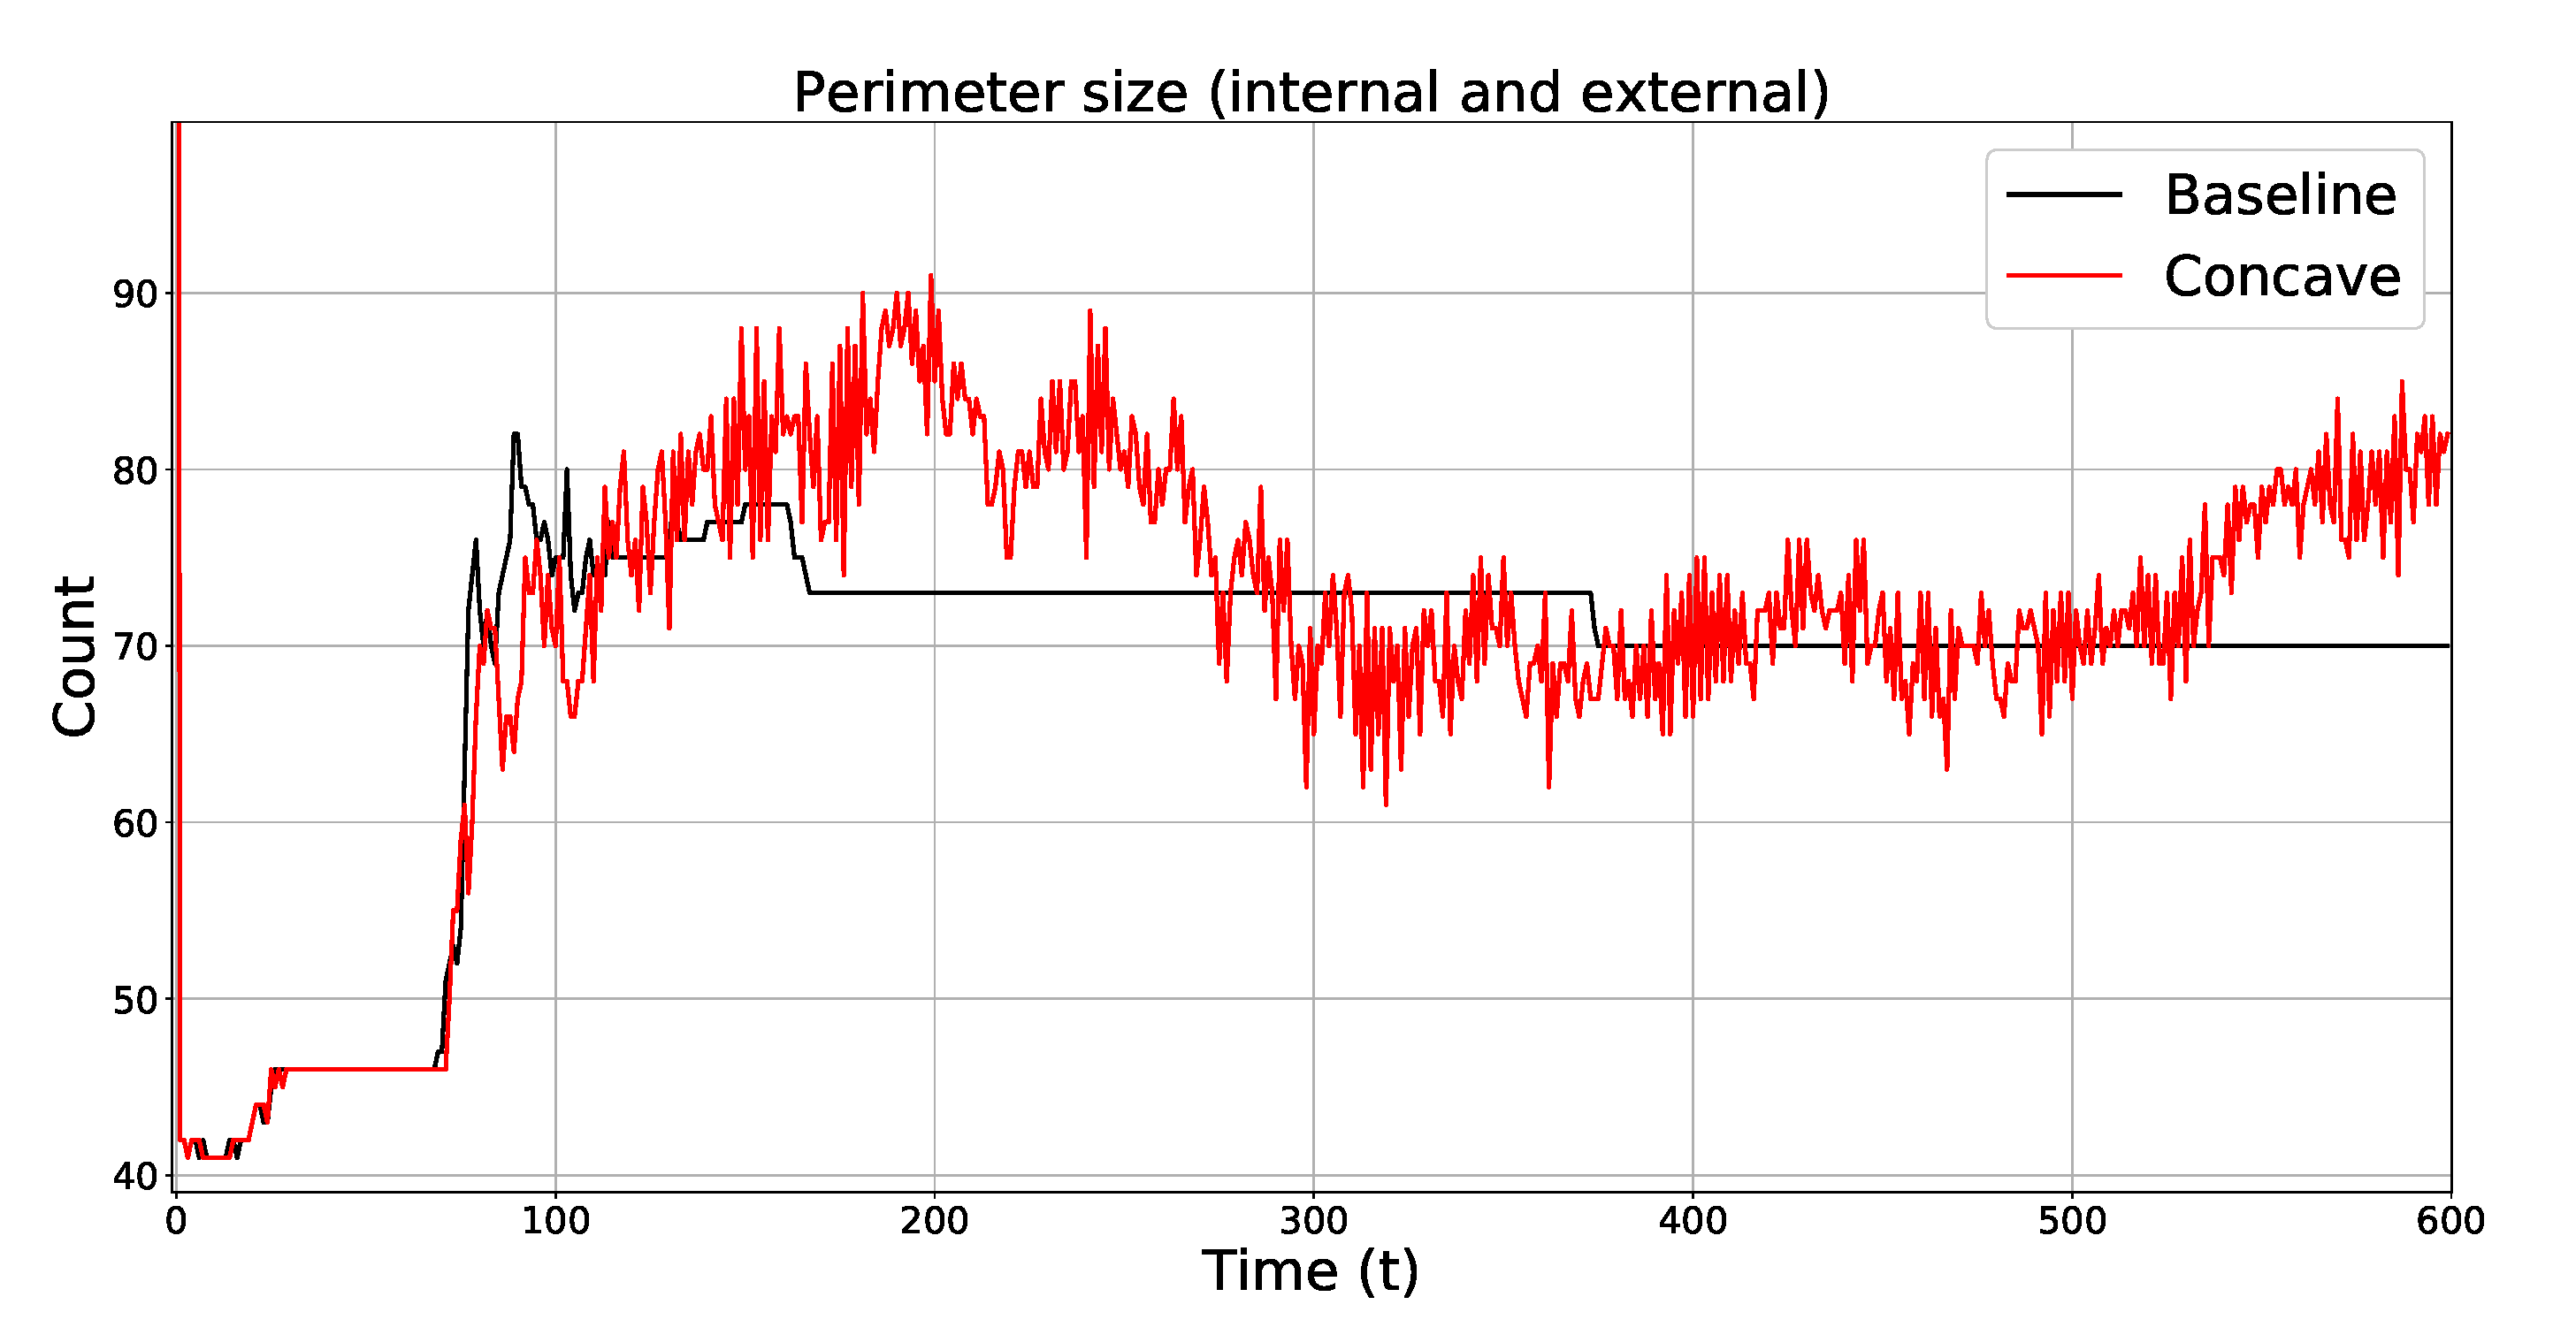
\includegraphics[width=8cm]{figures/BaselineConcavePerimeter}
%% \end{center}
%% \caption{Baseline/Concave perimeter size\label{concave:BaselineConcavePerimeter}}
%% \end{figure}
The effect on the structure of the swarm caused by the concave perimeter agents moving towards the gap agents is to pull the internal agents forward. This pulling causes the swarm to develop a more rounded structure but the effect also have a negative impact. If the tolerance of the agent's movements (the difference between the agent ranges for repulsion and cohesion) is too small then the distortion effect of the concave reduction can create additional voids. The perimeter agents will then move so as to remove the defect~(Fig.~\ref{fig:OuterPerimeterJitter1}). Following the void creation the agents are now impacted by a second concave reduction from the newly created void and the anomaly on the perimeter edge `snaps' back closing the void~(Fig.~\ref{fig:OuterPerimeterJitter2}). This process repeats itself creating an instability in the number of perimeter agents which is highlighted in~Fig.~\ref{concave:BaselineConcavePerimeter} as the erratic change in the number of agents. 

\Figure[t!](topskip=0pt, botskip=0pt, midskip=0pt)[width=5cm]{figures/OuterPerimeterJitter1}{Snapping effect closed\label{fig:OuterPerimeterJitter1}}
%% \begin{figure}
%% \begin{center}
%% 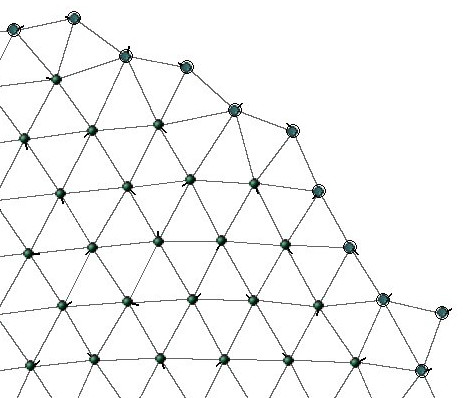
\includegraphics[width=5cm]{figures/OuterPerimeterJitter1}
%% \end{center}
%% \caption{Snapping effect closed\label{fig:OuterPerimeterJitter1}}
%% \end{figure}
\Figure[t!](topskip=0pt, botskip=0pt, midskip=0pt)[width=5cm]{figures/OuterPerimeterJitter2}{Snapping effect open\label{fig:OuterPerimeterJitter2}}
%% \begin{figure}
%% \begin{center}
%% 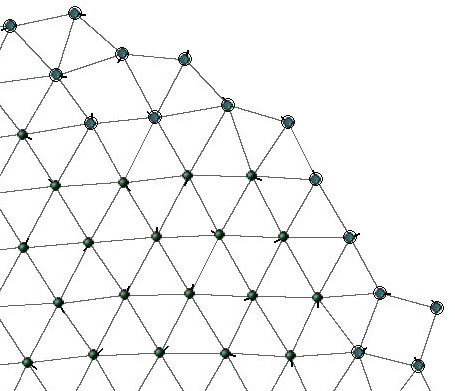
\includegraphics[width=5cm]{figures/OuterPerimeterJitter2}
%% \end{center}
%% \caption{Snapping effect open\label{fig:OuterPerimeterJitter2}}
%% \end{figure}
Figure~\ref{concave:BaselineConcaveEffectPath1} shows the paths of the agents in the swarm with concave reduction (red) and the baseline (black). The paths of the agents are initially very similar as the swarm expands but as the \textit{interaction vector magnitudes} rise and the swarm stabilises the effect of the \textit{concave reduction vectors} start to noticeably influence the swarm structure. The most noticeable effect is on the perimeter where the agents have expanded then instead of stabalising to relatively stable fixed position there is drifting effect occurring due to the imbalance of the initial deployment structure (more anomalies on one side). The swarm also becomes more `rounded' in appearance. 
%COVERBASELINE1.py

\Figure[t!](topskip=0pt, botskip=0pt, midskip=0pt)[width=8.3cm]{figures/BaselineConcaveEffectPath1}{Baseline/Concave path effect (Full)\label{concave:BaselineConcaveEffectPath1}}
%% \begin{figure}
%% \begin{center}
%% 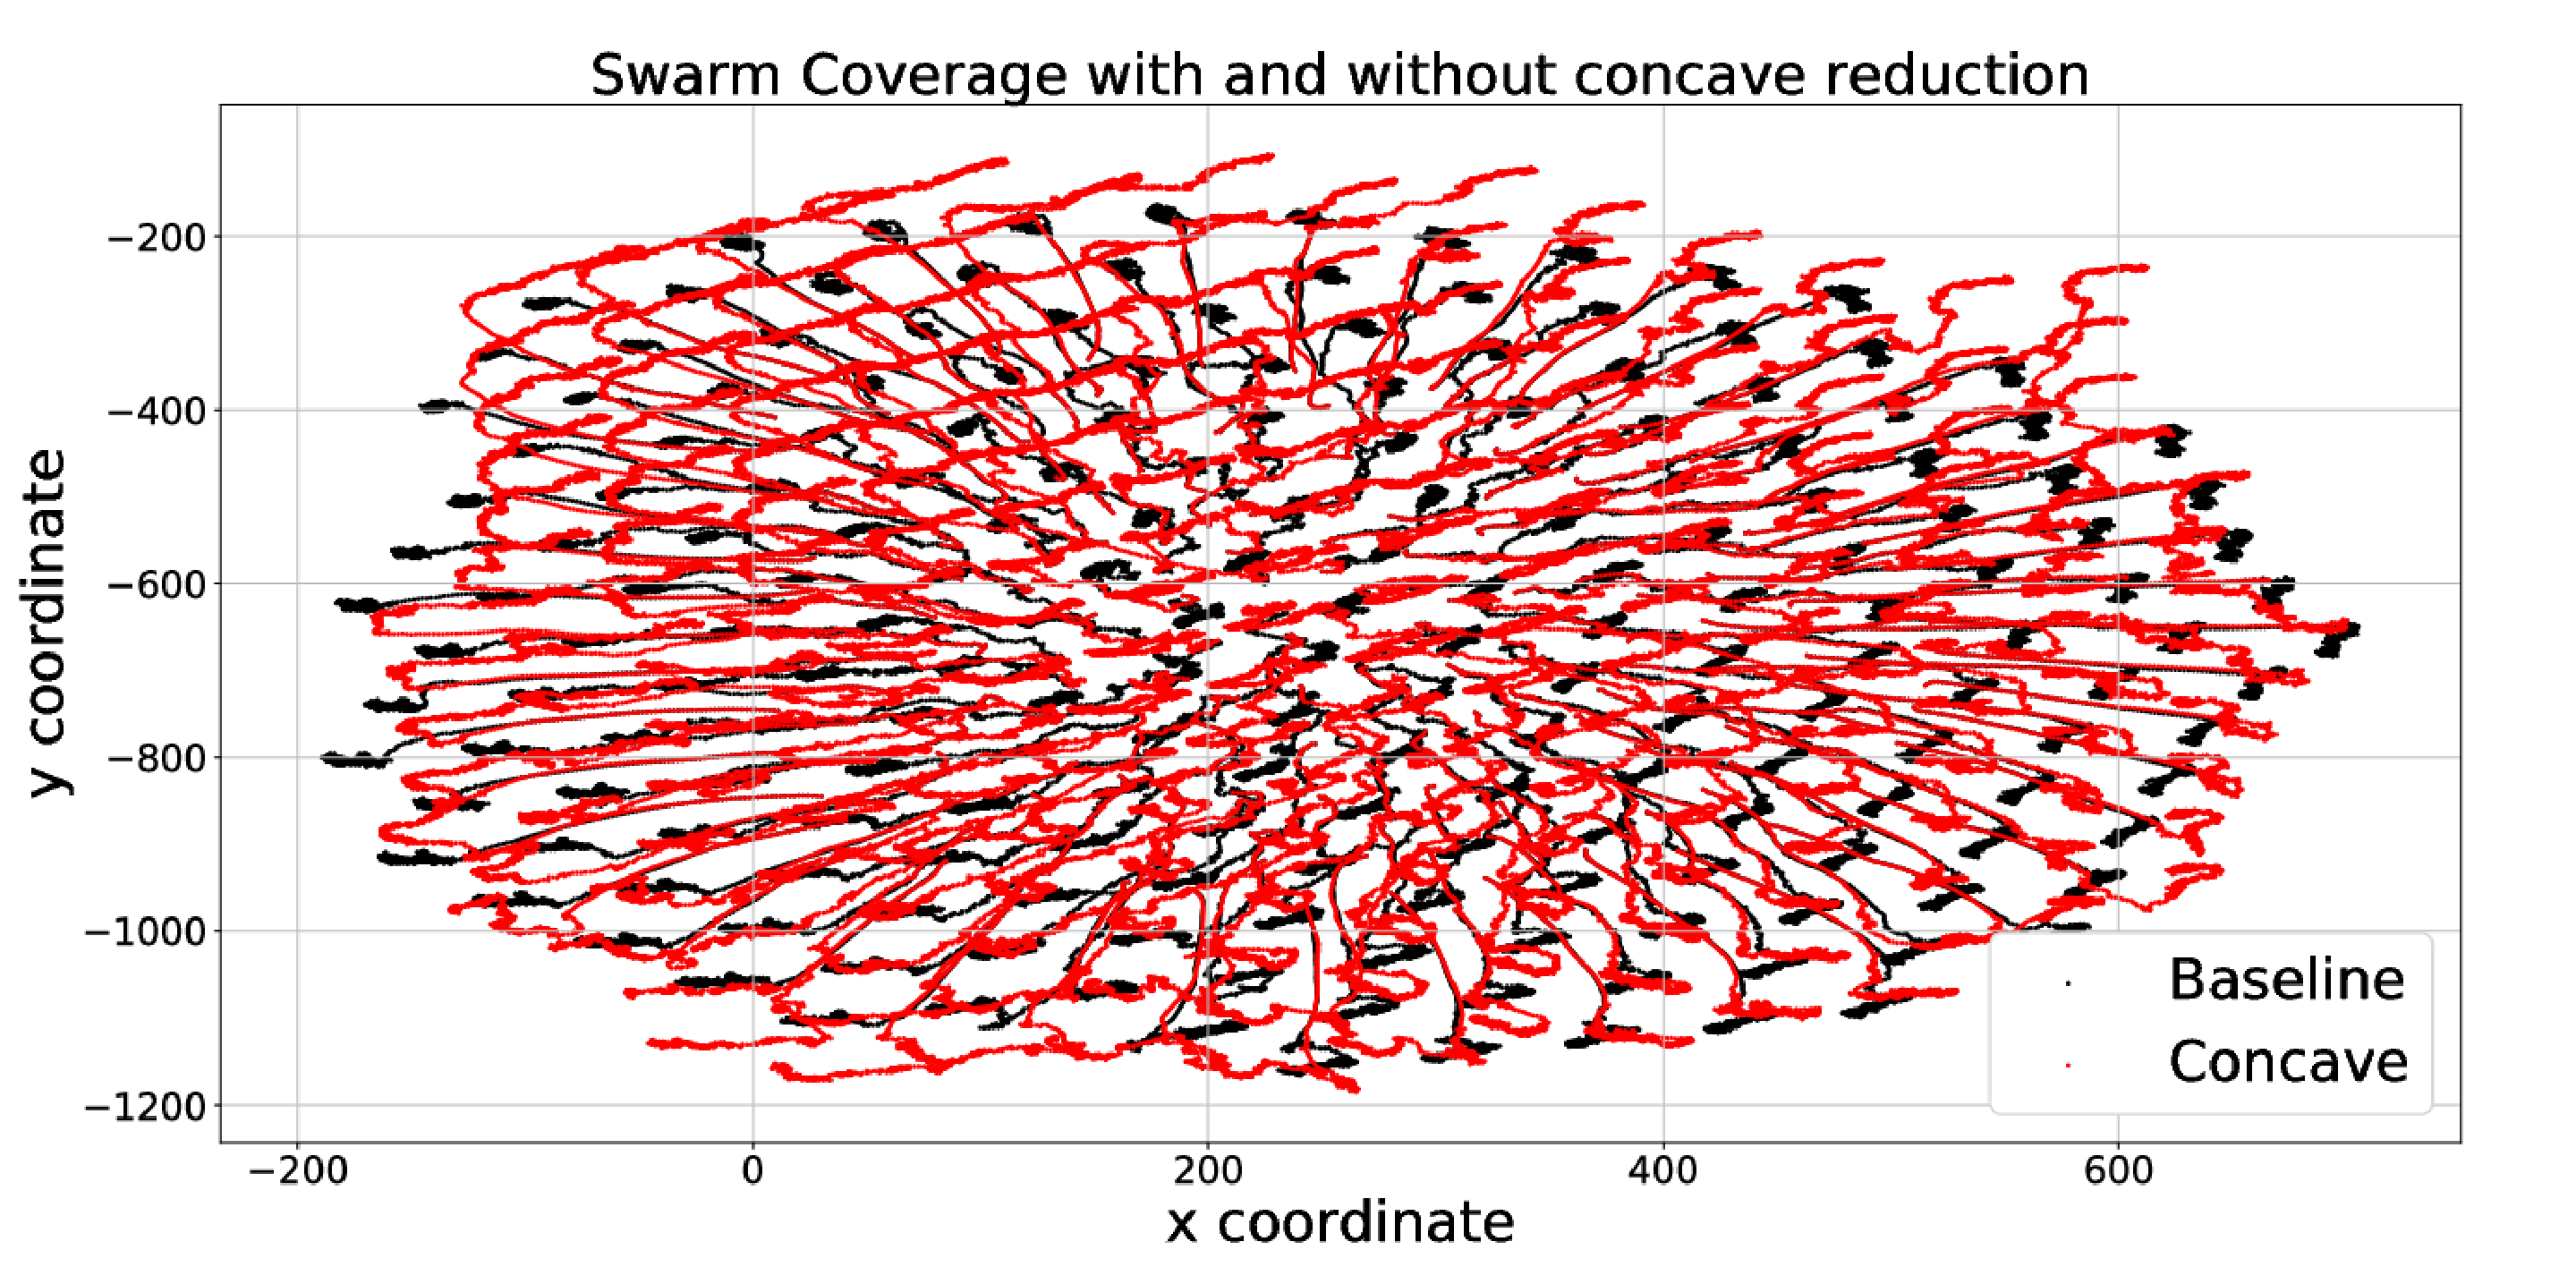
\includegraphics[width=8cm]{figures/BaselineConcaveEffectPath1}
%% \end{center}
%% \caption{Baseline/Concave path effect\label{concave:BaselineConcaveEffectPath1}}
%% \end{figure}

Figure~\ref{concave:BaselineConcaveEffectPath2} shows a more detailed view of the structure within the swarm. The baseline (black) paths show the swarm expanding and then settling to a hexagonal pattern which appears to oscillate slightly (jitter) when the swarm has reached its optimum distribution. The concave reduction swarm agents paths (red) show the swarm expanding in a similar way but once fully expanded the concave reduction causes the swarm to move with a slight directional bias.
%COVERBASELINE1.py

\Figure[t!](topskip=0pt, botskip=0pt, midskip=0pt)[width=8.3cm]{figures/BaselineConcaveEffectPath2}{Baseline/Concave path effect (Zoomed)\label{concave:BaselineConcaveEffectPath2}}
%% \begin{figure}
%% \begin{center}
%% 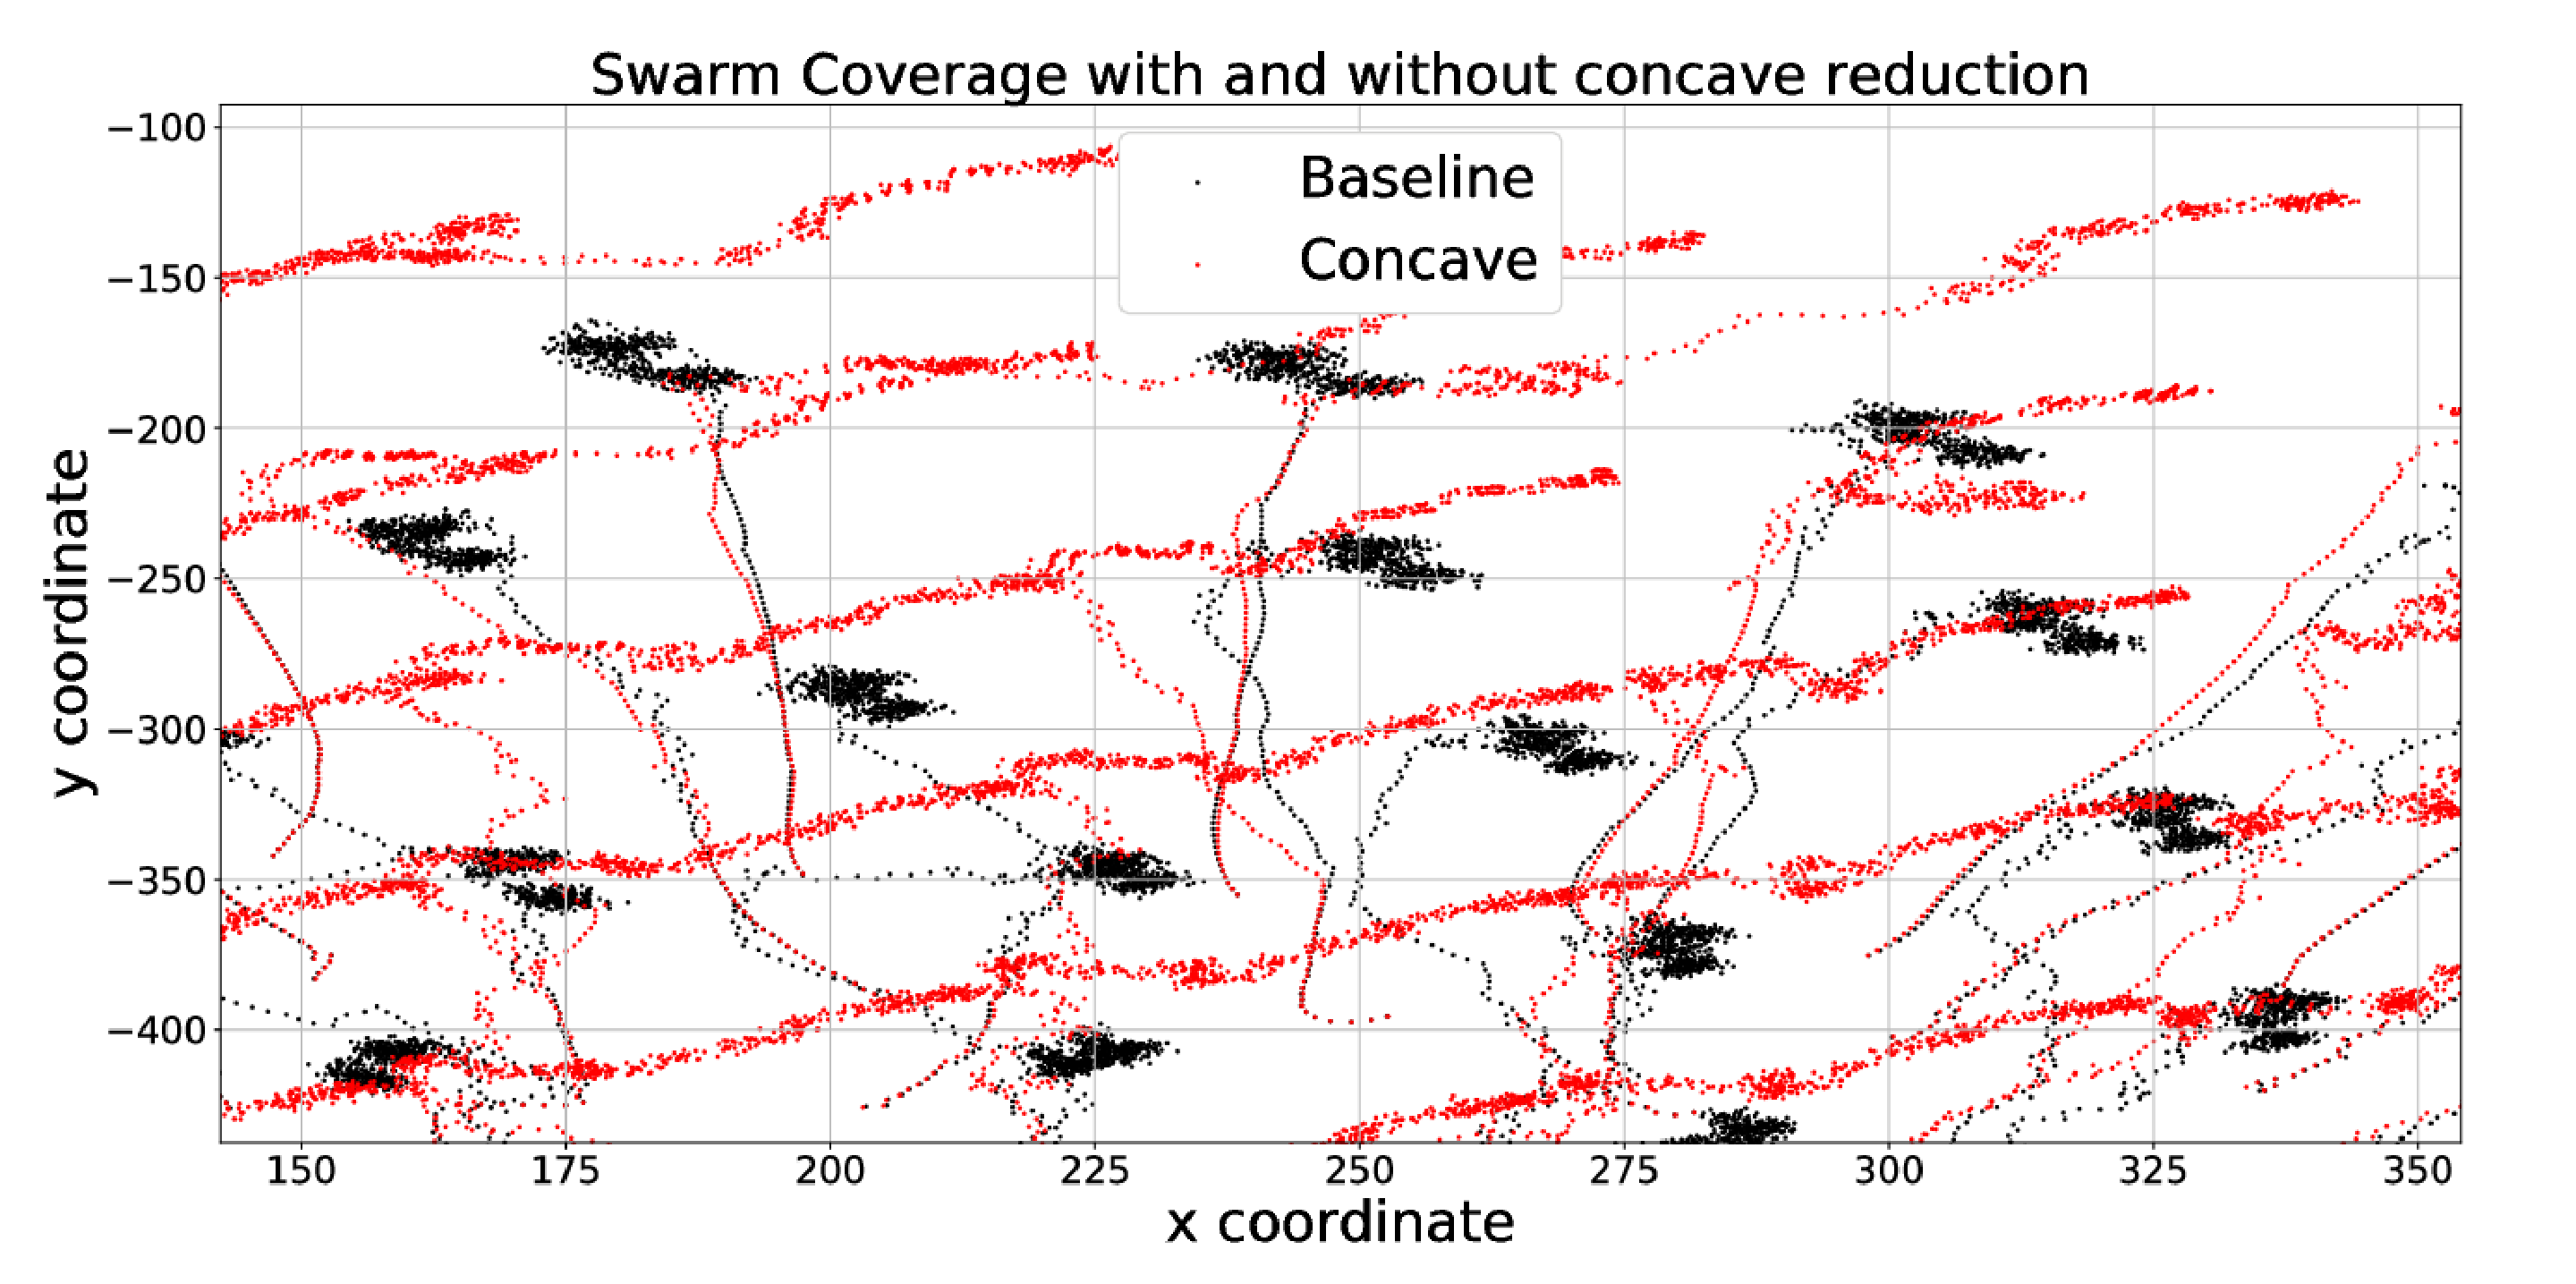
\includegraphics[width=8cm]{figures/BaselineConcaveEffectPath2}
%% \end{center}
%% \caption{Baseline/Concave path effect\label{concave:BaselineConcaveEffectPath2}}
%% \end{figure}

To reduce the `snapping' effect (shown in Fig.~\ref{fig:OuterPerimeterJitter1} and \ref{fig:OuterPerimeterJitter2}), the field effect parameters can be adjusted to create a greater tolerance in the agent interactions. This can be achieved by either reducing the agents repulsion field and maintaining the neighbour field effect or increasing the neighbour field effect and maintaining the repulsion field effect. These changes affect the structure of the swarm but ensure that the agents to stay within the cohesion field when moving to implement the concave reduction the agents are therefore `held' by the cohesion field effect preventing the `snap'. These changes in the field effect can be shown experimentally using the parameters in~Table~\ref{tab:BaselineConcaveReduction2}. 

\begin{table}
\caption{Baseline comparison for concave reduction} 
\label{tab:BaselineConcaveReduction2}
\begin{center}
\begin{tabular}{| p{1.4cm} | p{1.2cm} | p{1.2cm} | p{2.5cm} |}
\hline
\bf Weight \bf component & \bf Baseline \bf swarm & \bf Concave \bf reduction & \bf Description \\ \hline
Sample rate & 100 & 100 & ms - Unit sampling interval\\  \hline
$k_{cr}$ & 0 & 100 & weight adjuster for concave reduction vector\\  \hline
$k_c$ & 5 & 5 & weight adjuster for cohesion field\\  \hline
$k_r$ & 15 & 15 & weight adjuster for repulsion field\\  \hline
$k_d$ & 0 & 0 & weight adjuster for destination vector 0 for static baseline 100 from directional\\  \hline
Repulsion Boundary & 60 & 60 & units\\  \hline
Neighbour Distance & 80 & 80 & units\\  \hline
Speed & 20 & 20 & units/s\\  \hline
\end{tabular}
\end{center}
\end{table}

Figure~\ref{concave:BaselineConcaveEffectDist8060} shows a comparison of the agent movements based on distance for the revised field effects. The graph shows that the swarm settles to a distance that is closer due to the reduced repulsion field. The graph also shows that the concave reduction still induces additional jitter as the variance is still greater than the baseline but due to the reduced snapping the perimeter agent count shows greater stability~(\ref{concave:BaselineConcavePerimeter8060}). 
%BASELINE-COMPRESS-DIST-8060.py

\Figure[t!](topskip=0pt, botskip=0pt, midskip=0pt)[width=8.3cm]{figures/BaselineConcaveEffectDist8060}{Baseline/Concave effect distance (80/60)\label{concave:BaselineConcaveEffectDist8060}}
%% \begin{figure}
%% \begin{center}
%% 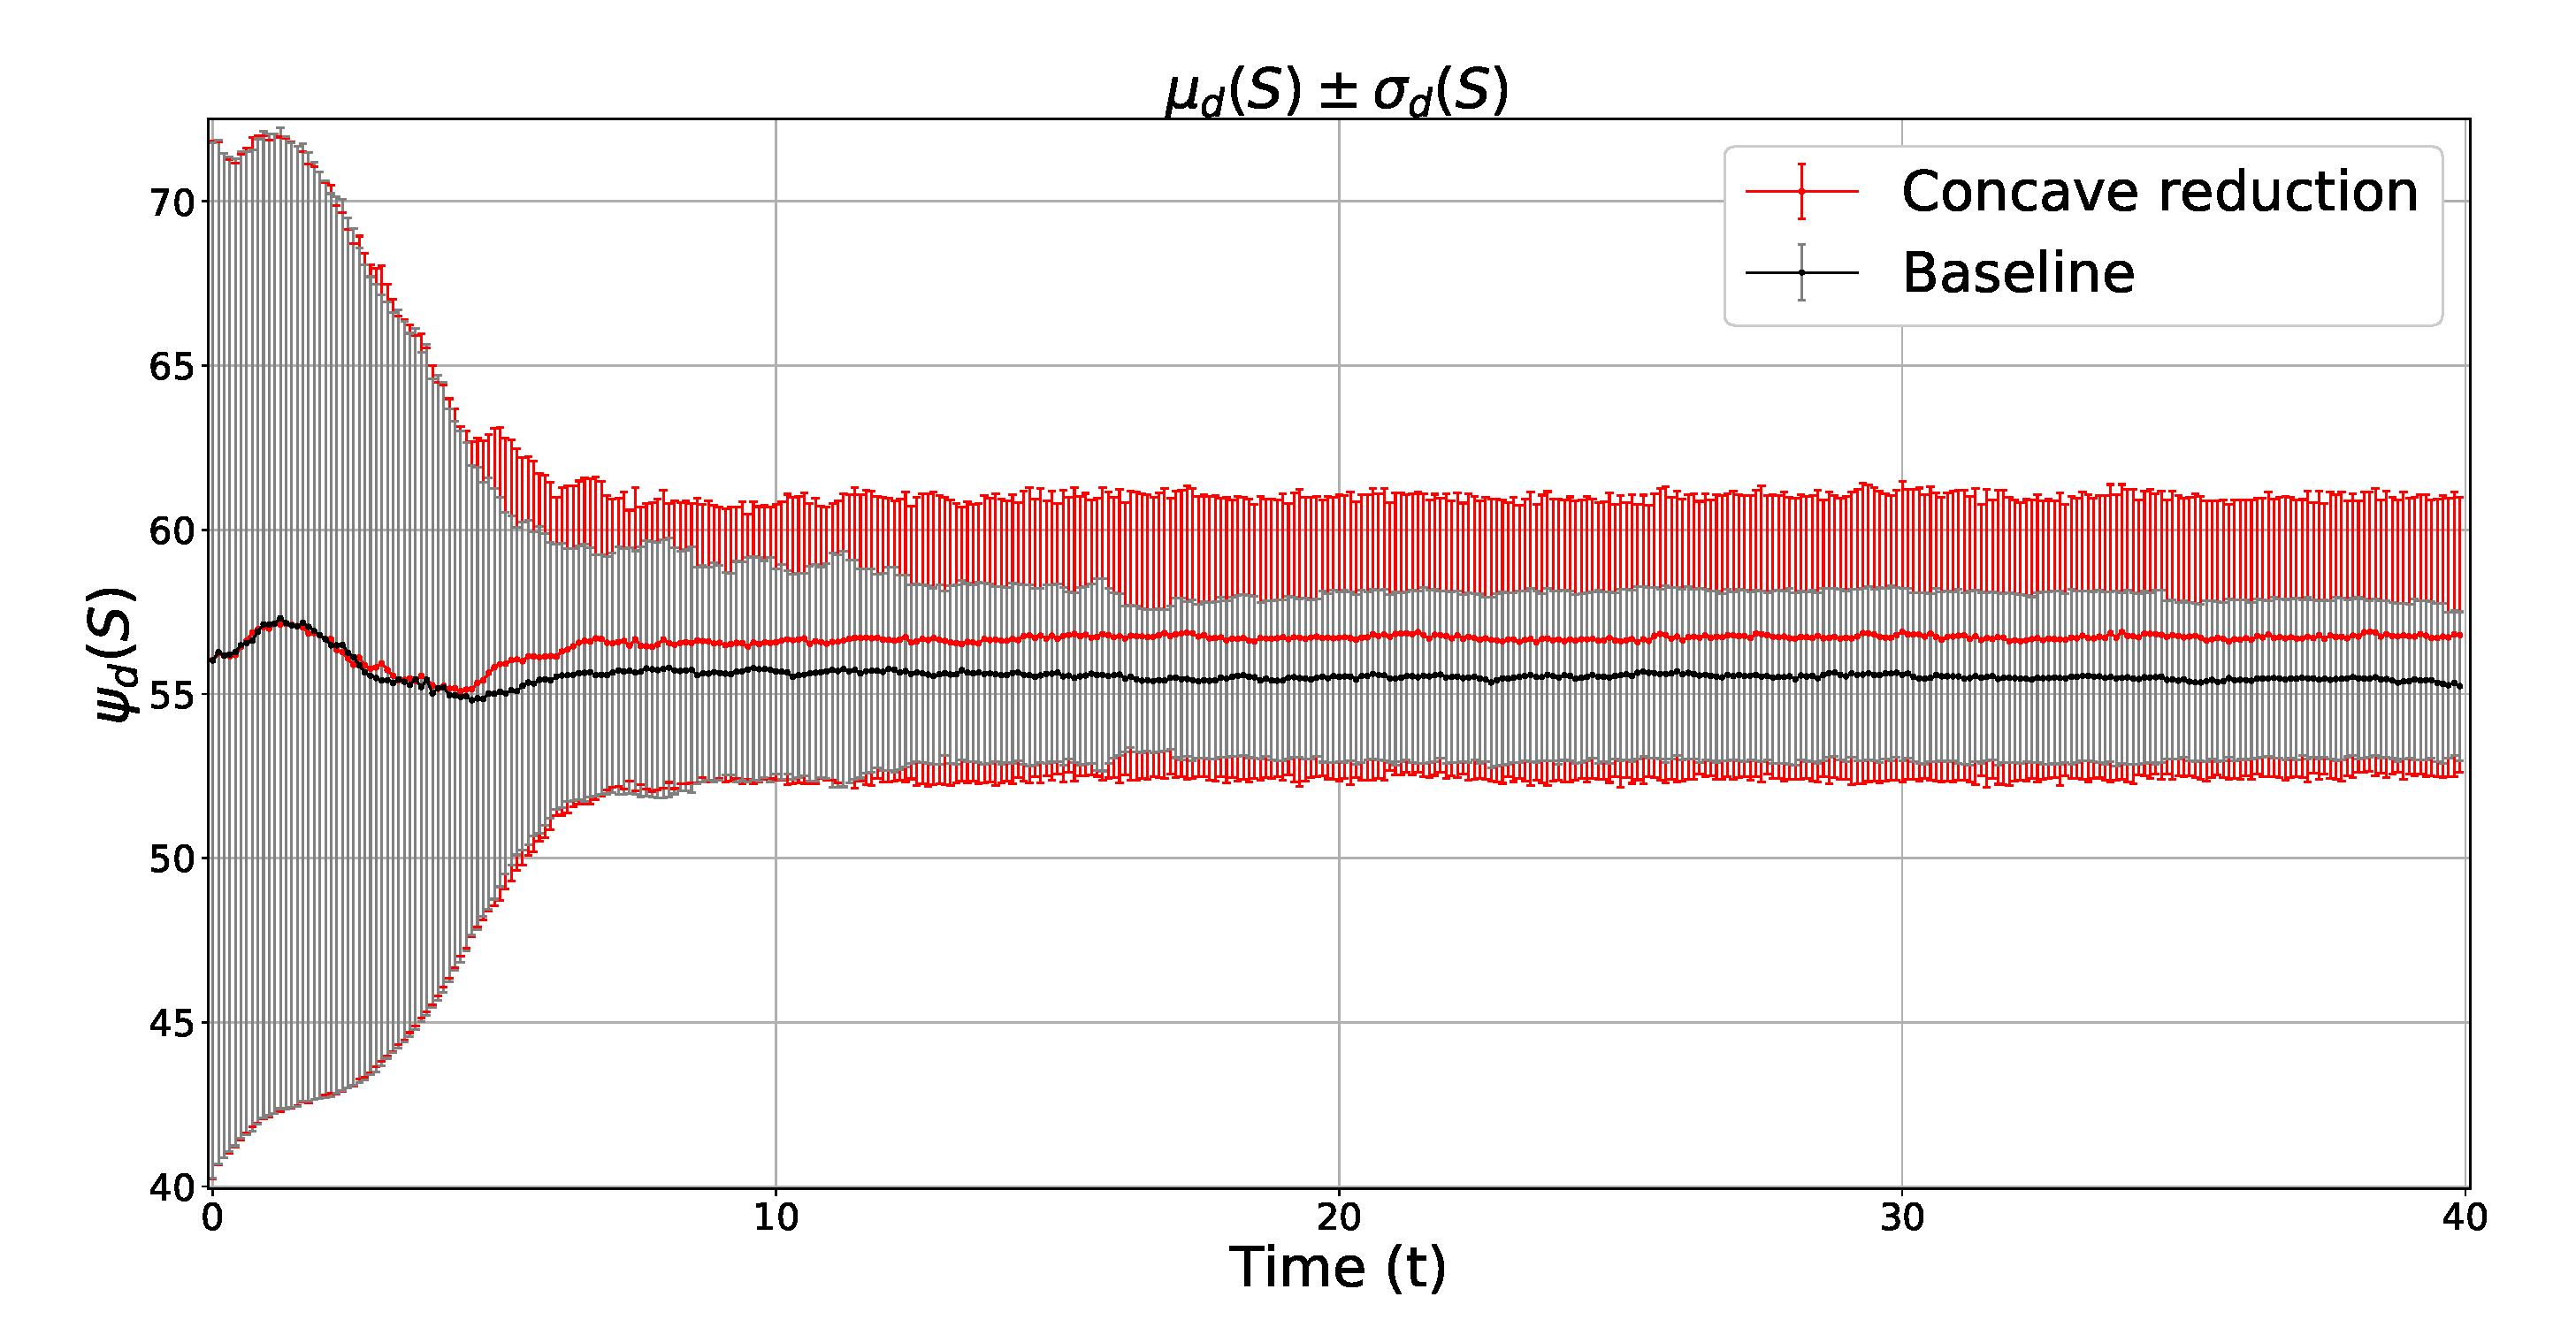
\includegraphics[width=8cm]{figures/BaselineConcaveEffectDist8060}
%% \end{center}
%% \caption{Baseline/Concave effect distance (80/60)\label{concave:BaselineConcaveEffectDist8060}}
%% \end{figure}

Figure~\ref{concave:BaselineConcaveEffectMag8060} shows that the \textit{inter-agent vector magnitude} is reduced due to the reduced cohesion from the agent proximity and the \textit{concave reduction vector magnitude} impact is reduced due to less anomalies occurring on the perimeter.
%BASELINE-COMPRESS-MAG-8060.py

\Figure[t!](topskip=0pt, botskip=0pt, midskip=0pt)[width=8.3cm]{figures/BaselineConcaveEffectMag8060}{Baseline/Concave effect magnitude (80/60)\label{concave:BaselineConcaveEffectMag8060}}
% \begin{figure}
% \begin{center}
% 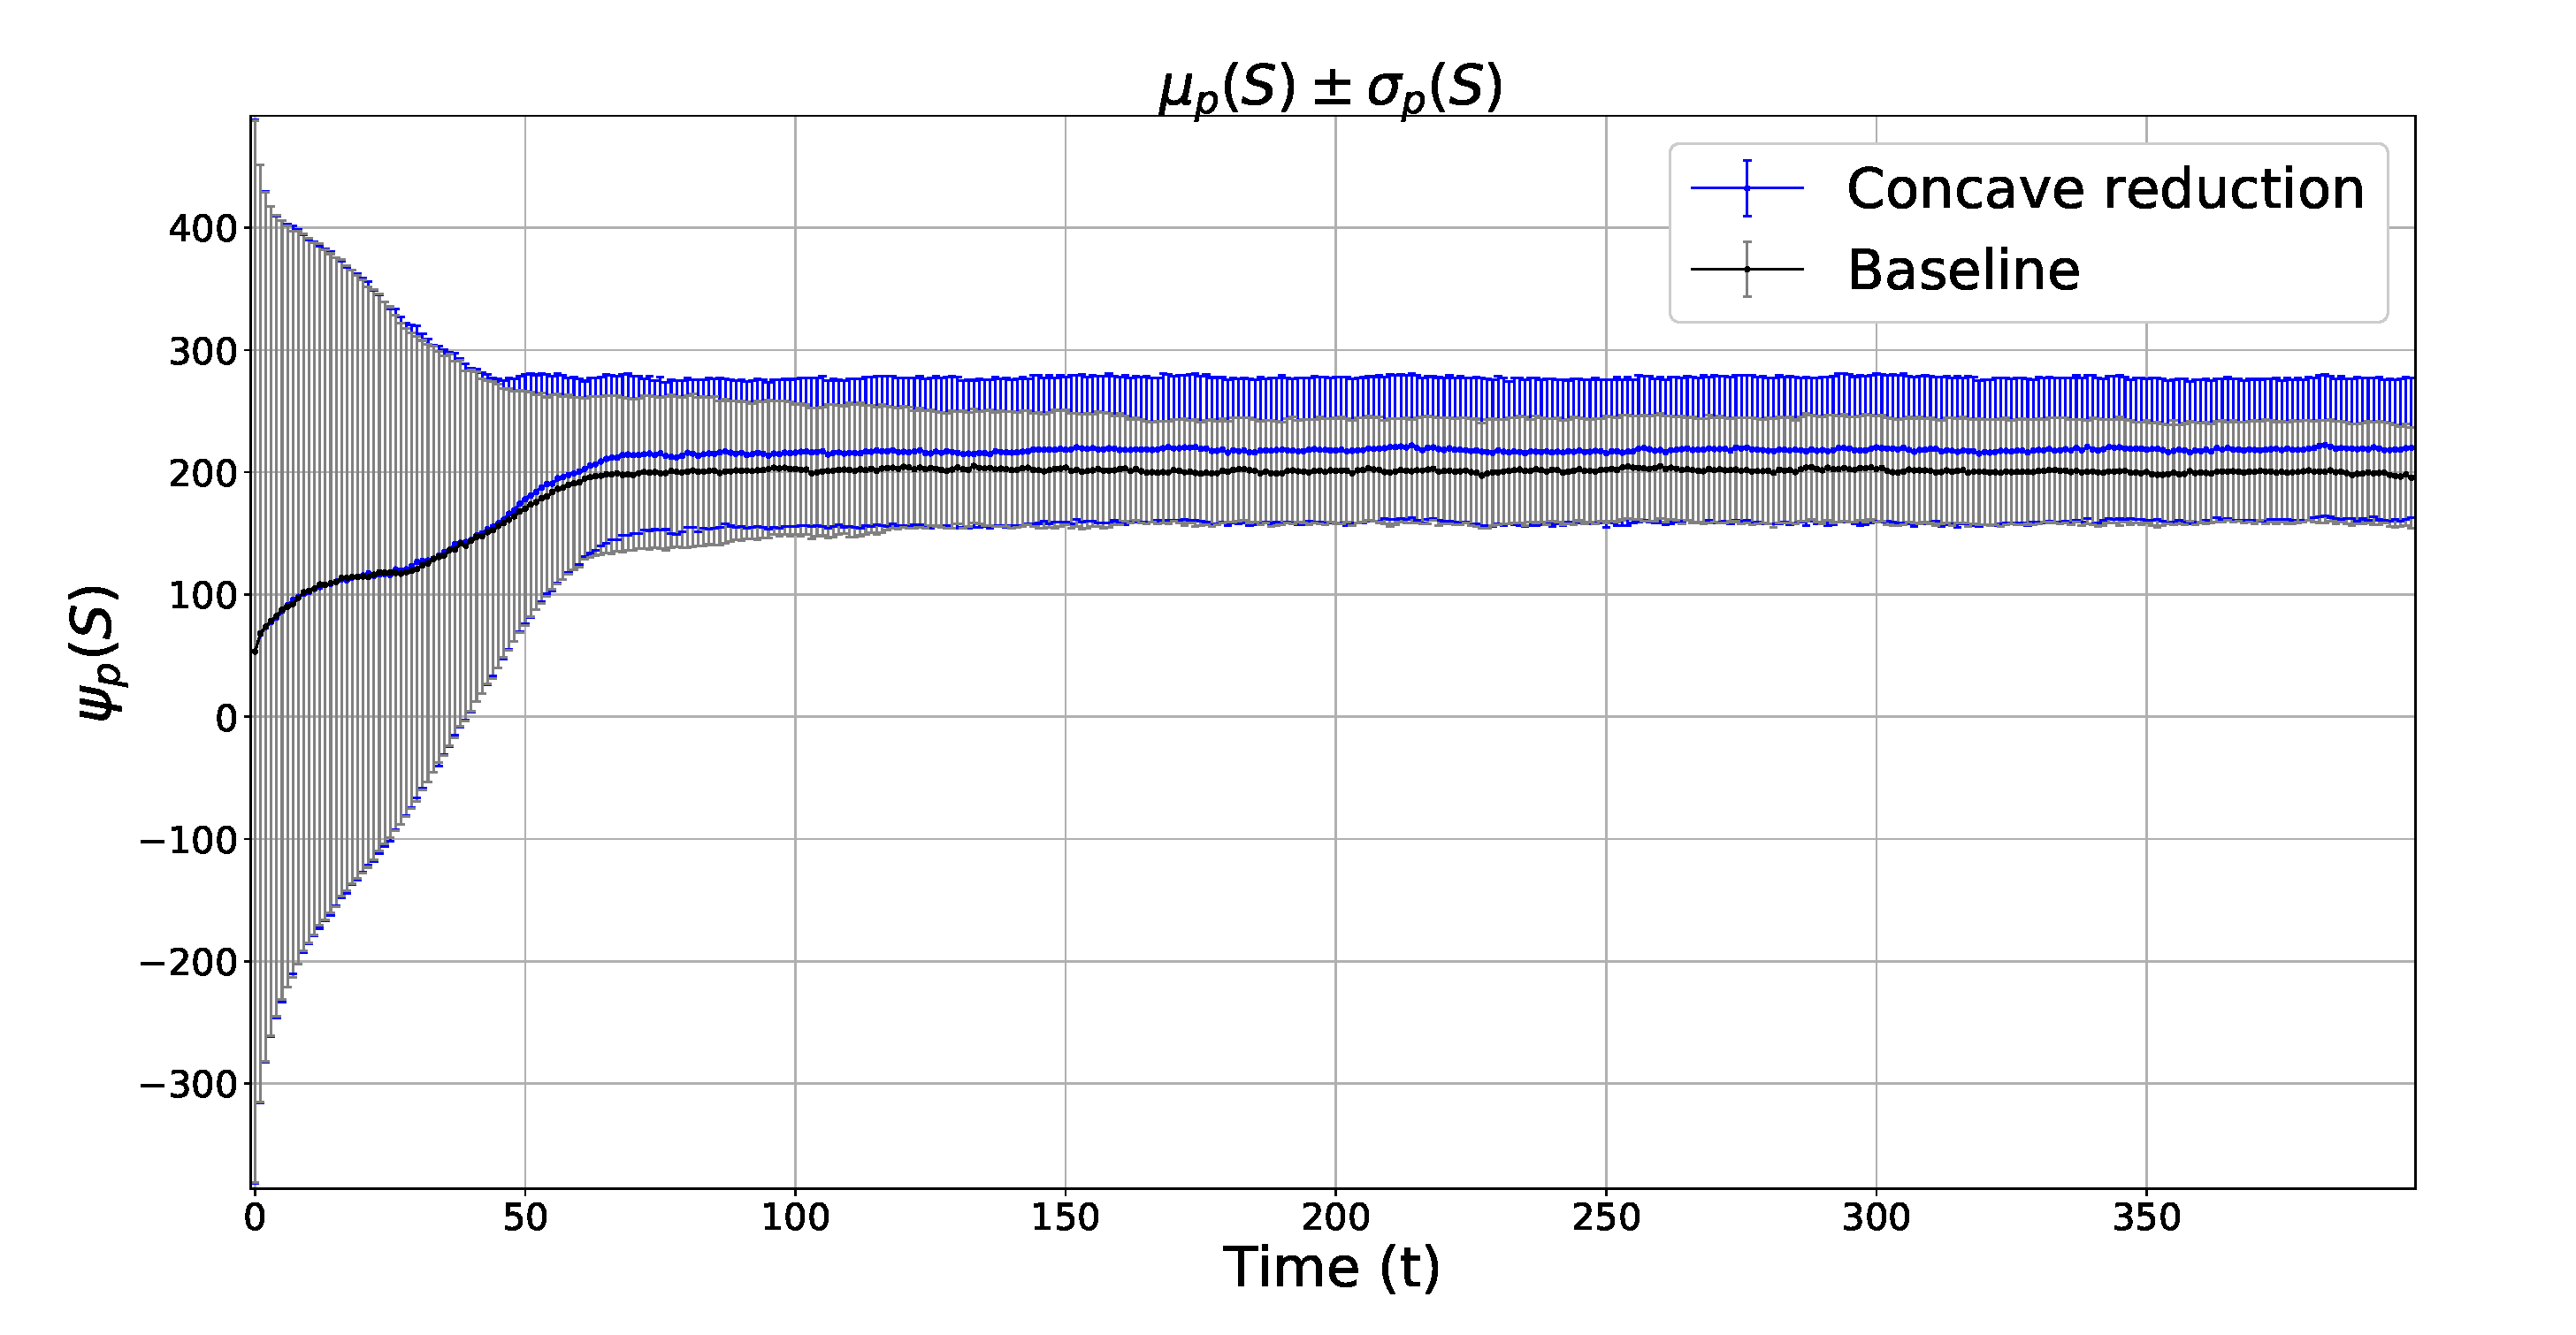
\includegraphics[width=8cm]{figures/BaselineConcaveEffectMag8060}
% \end{center}
% \caption{Baseline/Concave effect magnitude (80/60)\label{concave:BaselineConcaveEffectMag8060}}
% \end{figure}

Figure~\ref{concave:BaselineConcavePerimeter8060} shows the changes in the perimeter size from the baseline and the concave reduction swarms. The concave reduction still creates an erratic perimeter count but the variation is reduced. On aggregate for the run the concave reduction has reduced the perimeter size. The revised effects also reduce the snapping effect and the swarm has an improved structure. The concave reduction creates a perimeter which fluctuates between 45-50 agents where as the baseline swarm settles to 49 agents.
%PERIMETER8060CONCAVE.py

\Figure[t!](topskip=0pt, botskip=0pt, midskip=0pt)[width=8.3cm]{figures/BaselineConcavePerimeter8060}{Baseline/Concave perimeter size (80/60)\label{concave:BaselineConcavePerimeter8060}}
%% \begin{figure}
%% \begin{center}
%% 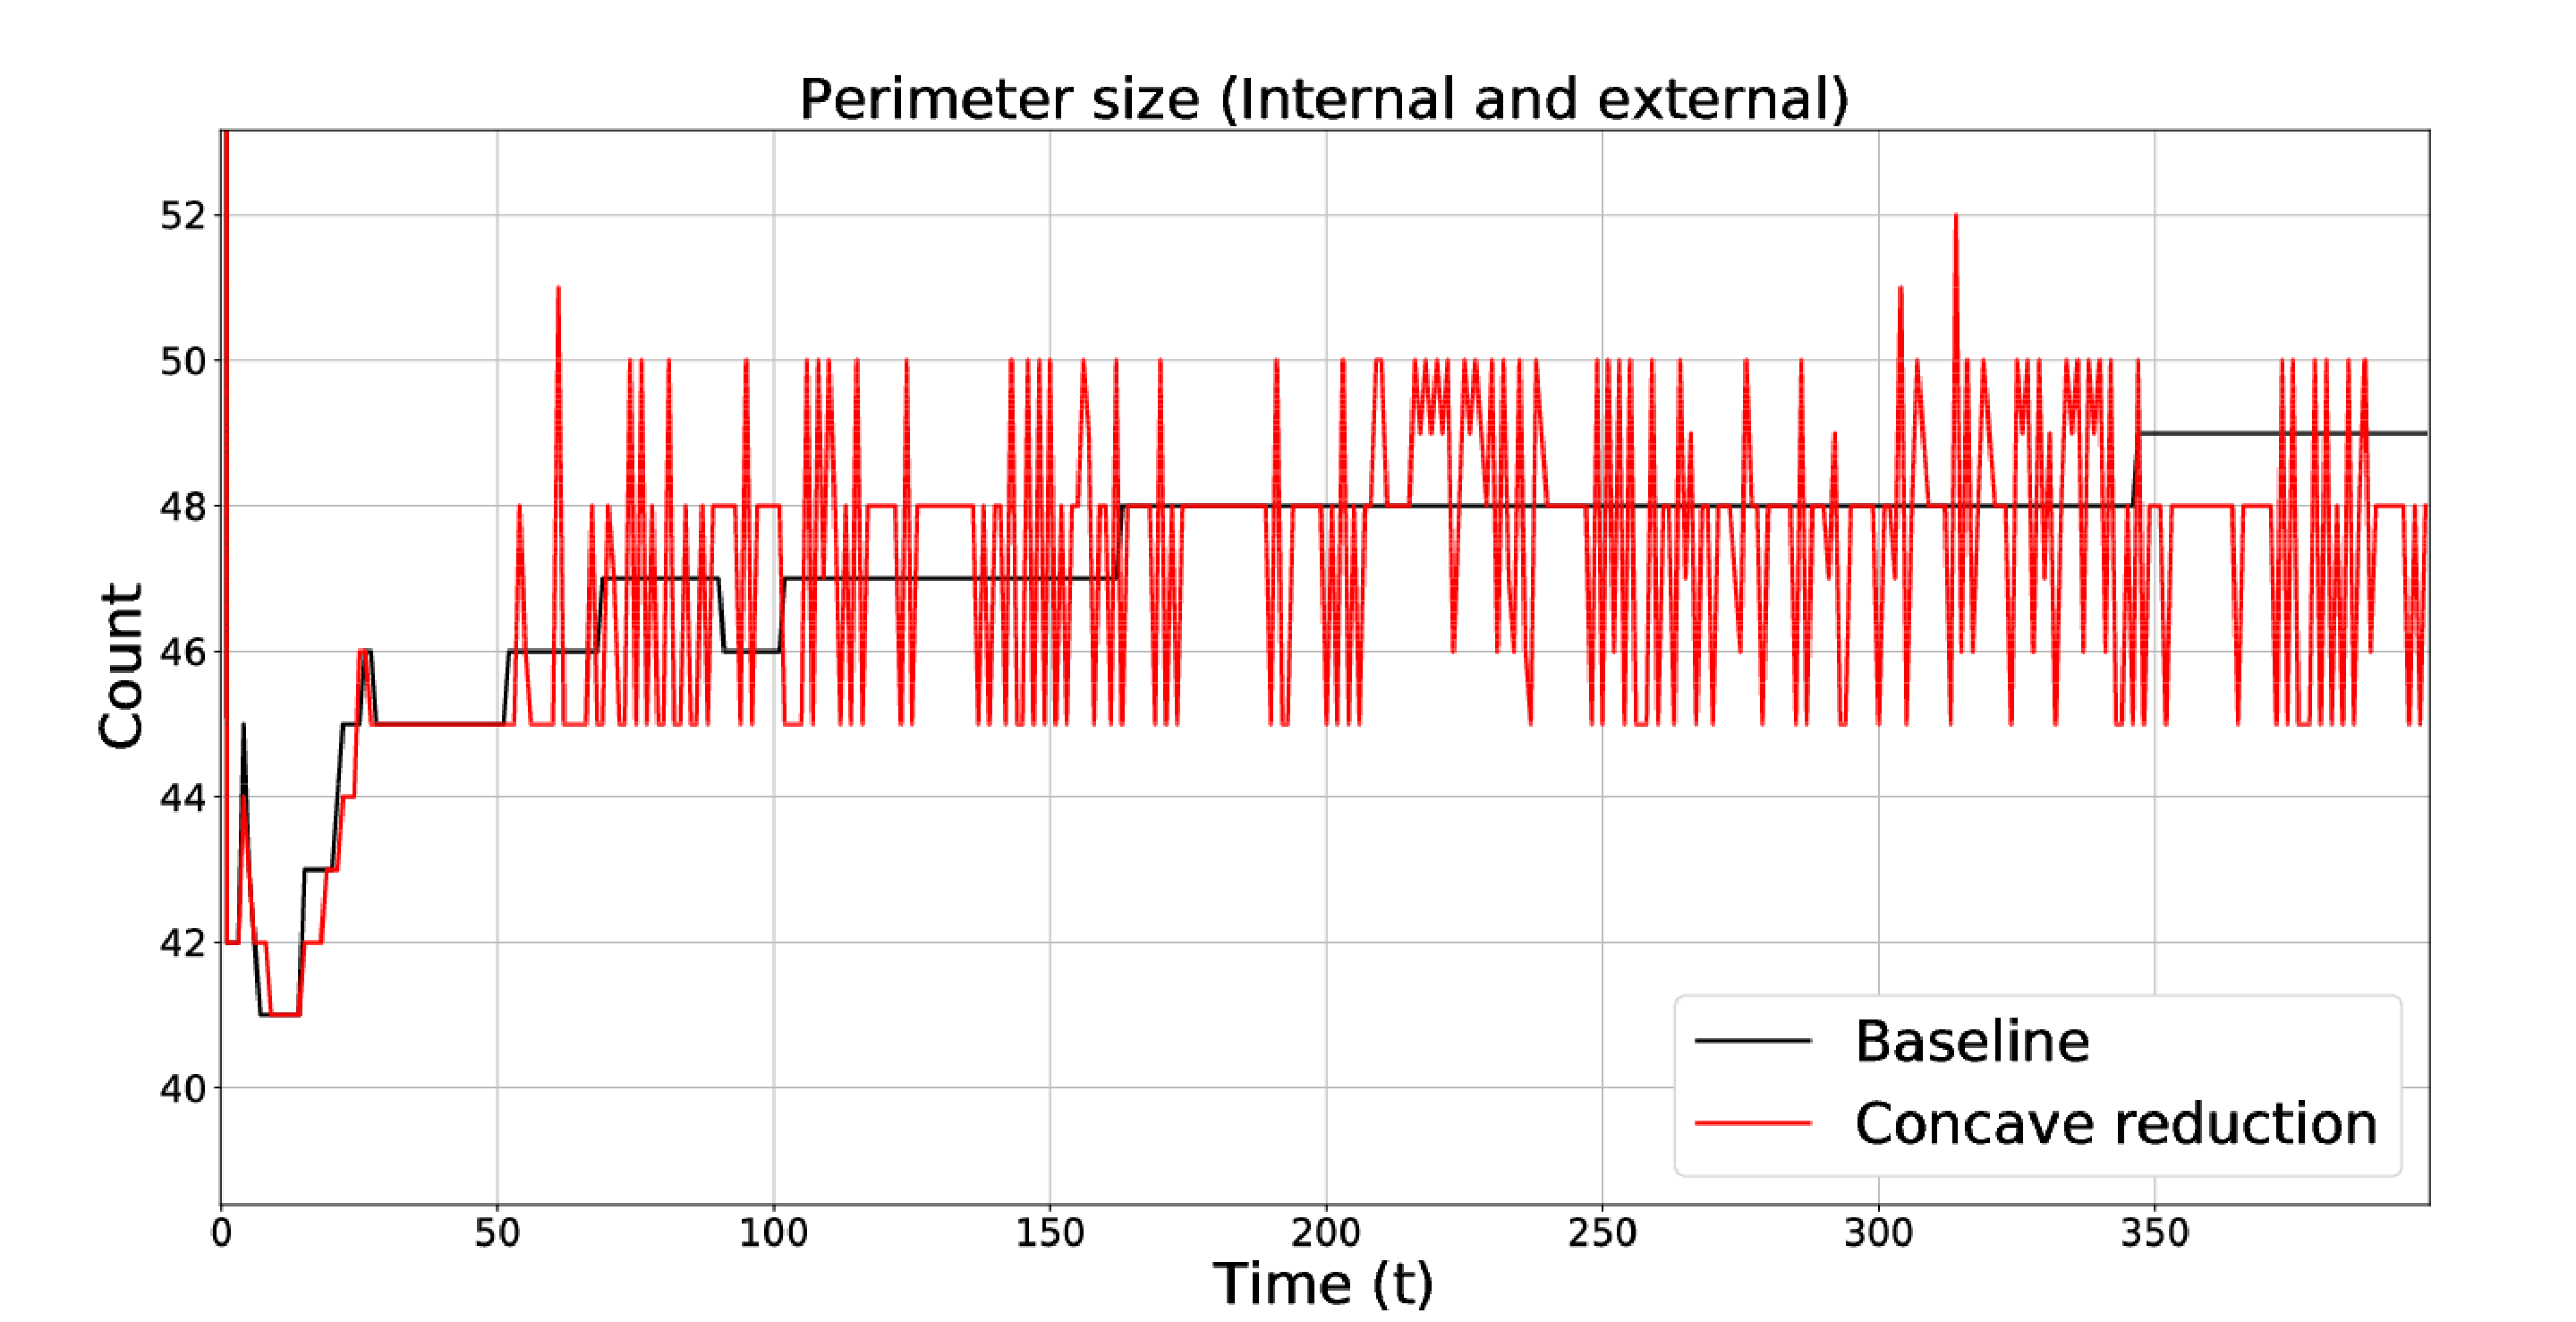
\includegraphics[width=8cm]{figures/BaselineConcavePerimeter8060}
%% \end{center}
%% \caption{Baseline/Concave perimeter size (80/60)\label{concave:BaselineConcavePerimeter8060}}
%% \end{figure}

For the period of the simulation the baseline had 19049 perimeter agents and the concave reduction had 18940 which is an improvement of 0.5\% overall for the whole simulation. This is only a small change in the perimeter size but the impact on the swarm structure is significant. The \textit{concave reduction vectors} have `pulled' the swarm into a more circular shape~\ref{fig:ConcaveEndPoint}.
%COVERBASELINE8060END.py

\Figure[t!](topskip=0pt, botskip=0pt, midskip=0pt)[width=8.3cm]{figures/Baseline8060End}{Baseline end\label{fig:BaselineEndPoint}}
%% \begin{figure}
%% \begin{center}
%% 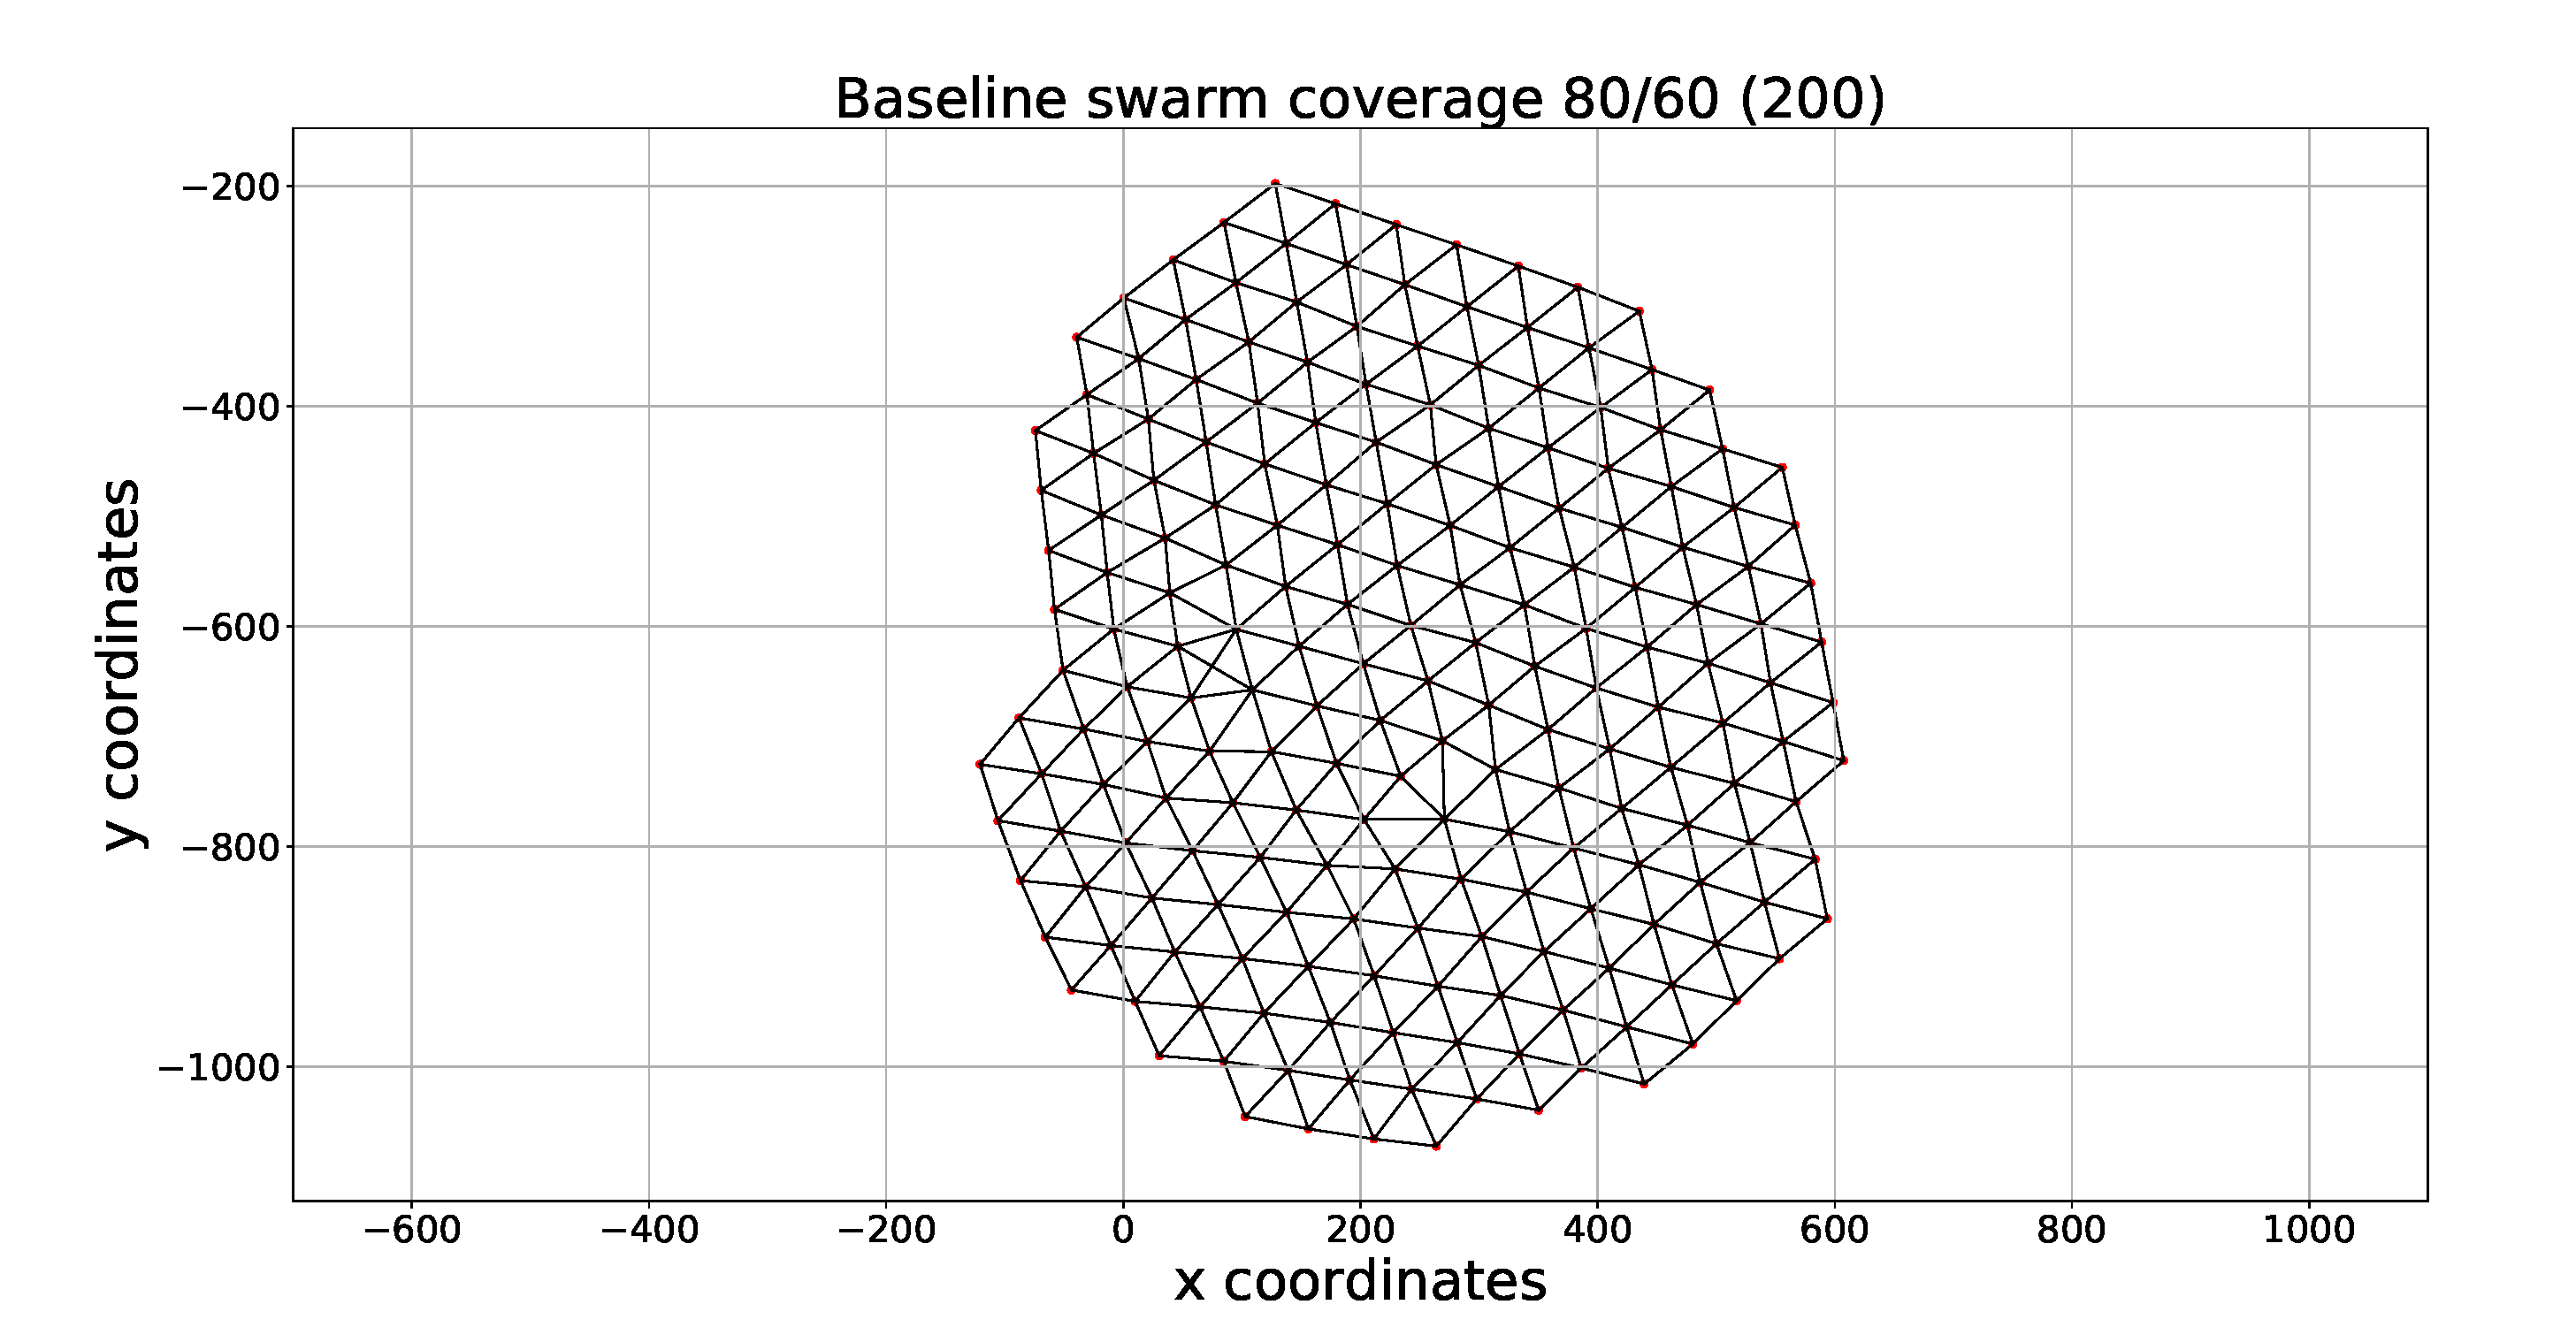
\includegraphics[width=8cm]{figures/Baseline8060End}
%% \end{center}
%% \caption{Baseline end\label{fig:BaselineEndPoint}}
%% \end{figure}
%COVERBASELINE8060COMPRESSEND.py
\Figure[t!](topskip=0pt, botskip=0pt, midskip=0pt)[width=8.3cm]{figures/Concave8060End}{Concave reduction end\label{fig:ConcaveEndPoint}}
%% \begin{figure}
%% \begin{center}
%% 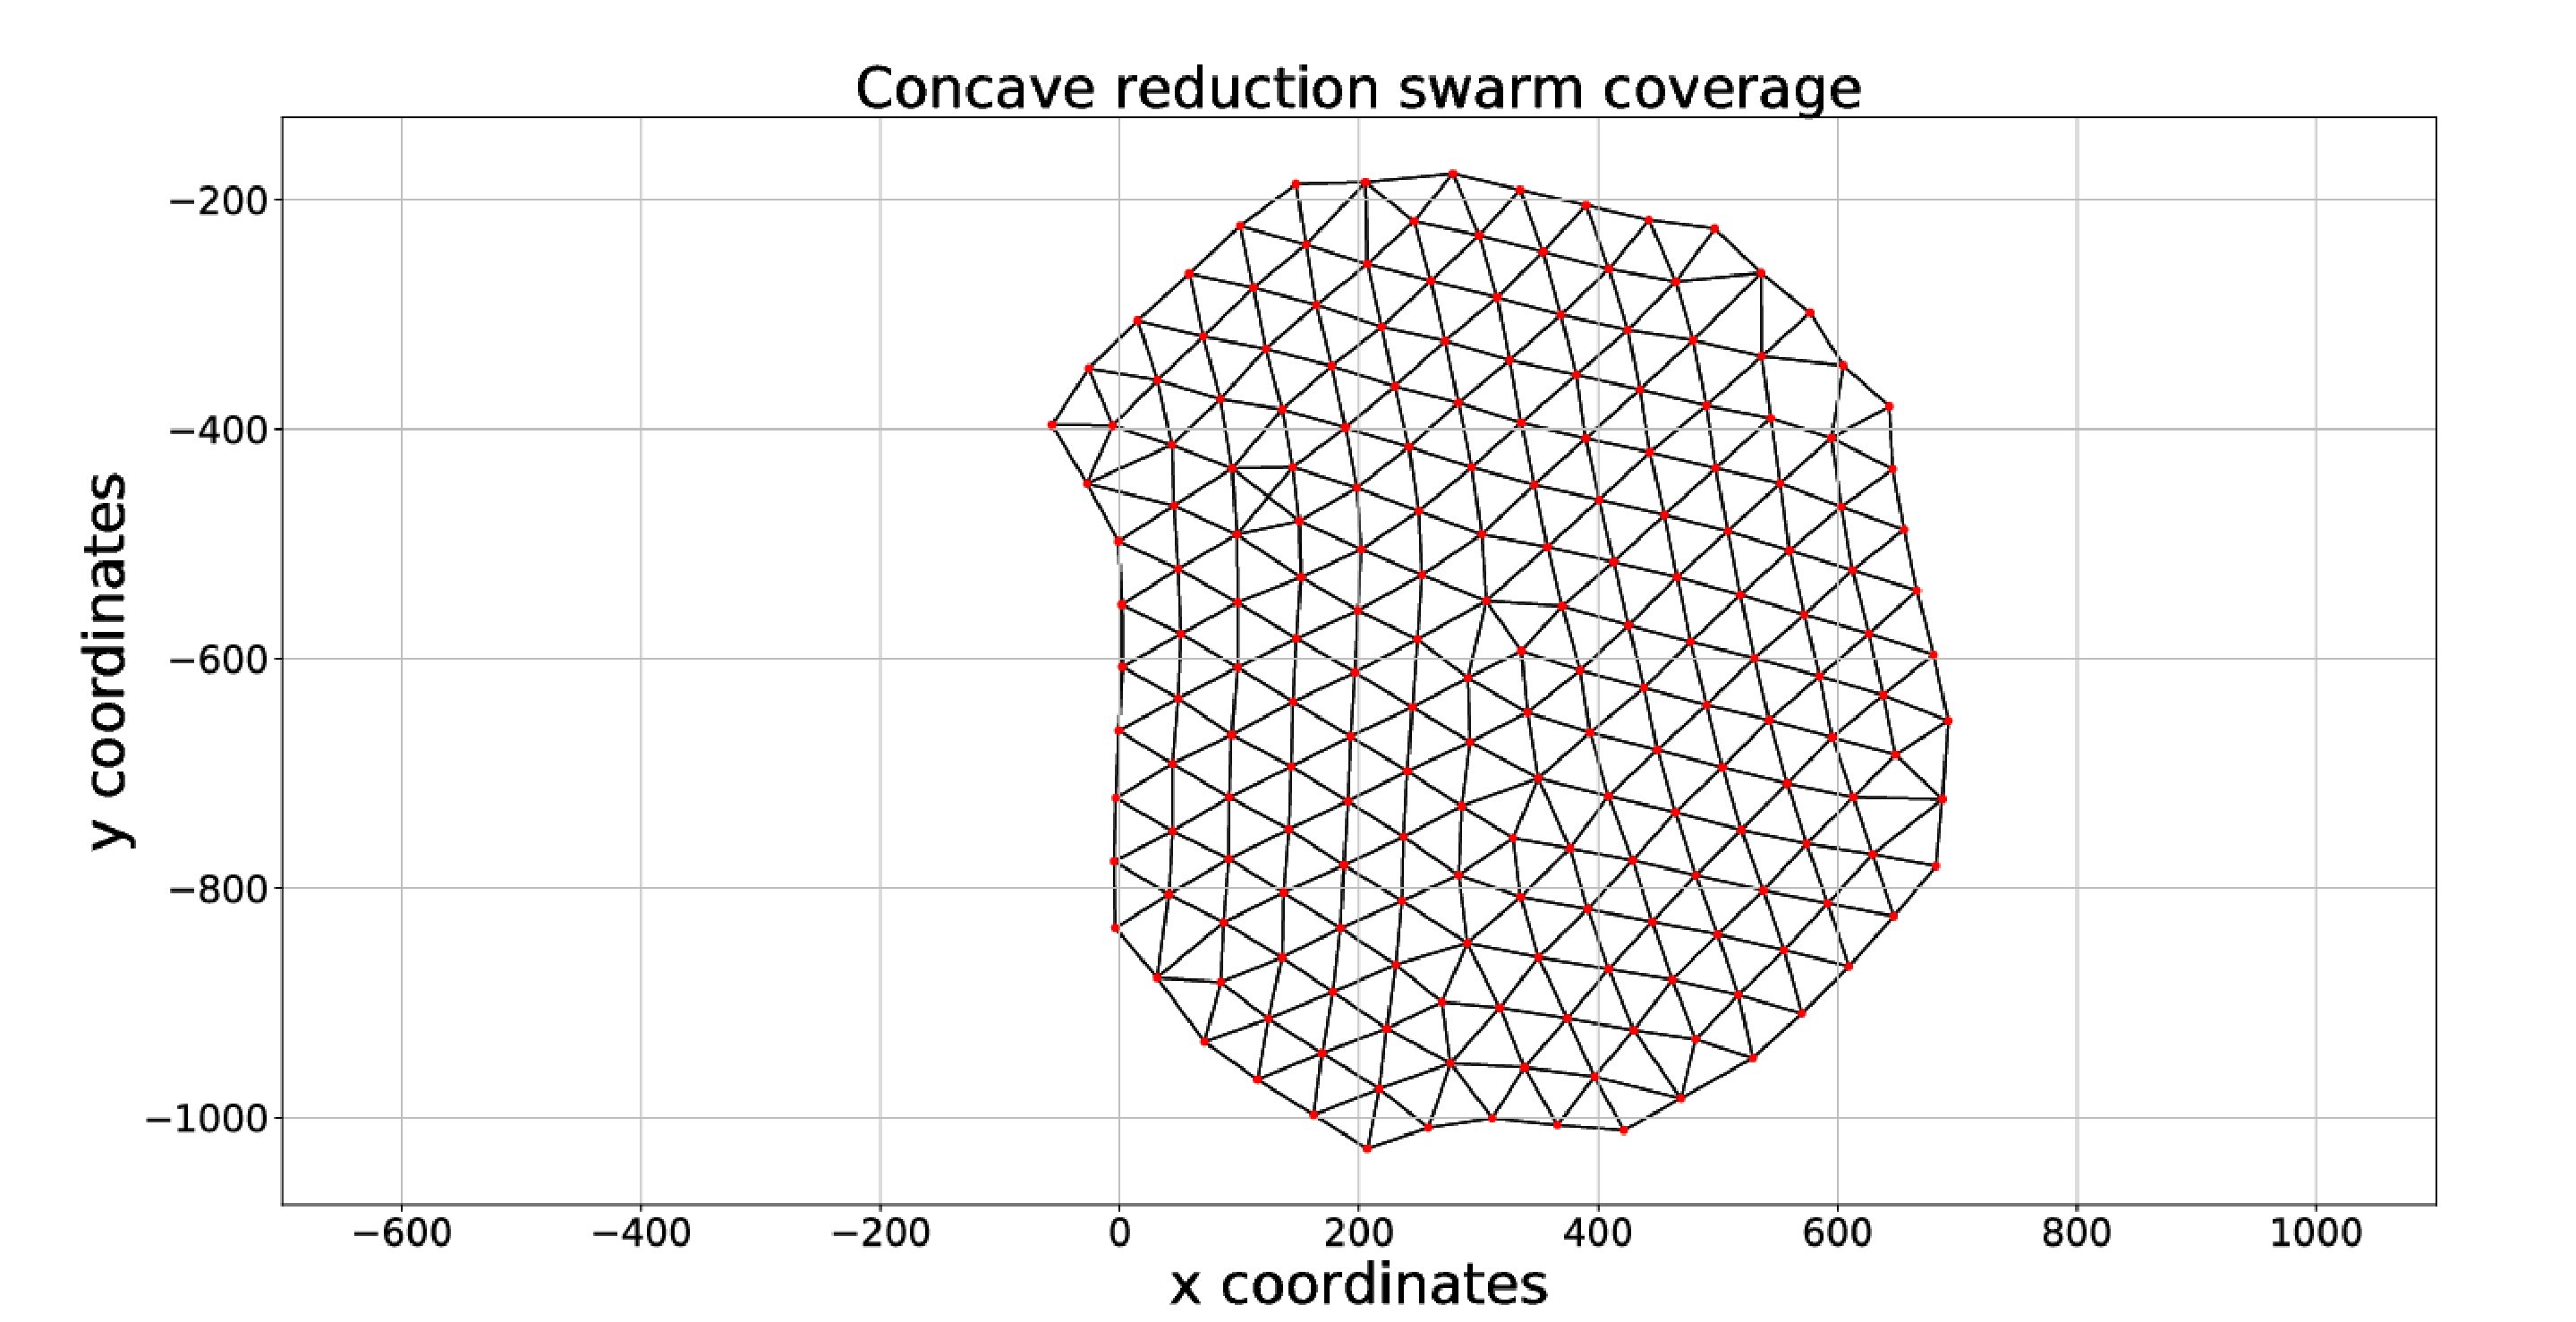
\includegraphics[width=8cm]{figures/Concave8060End}
%% \end{center}
%% \caption{Concave reduction end\label{fig:ConcaveEndPoint}}
%% \end{figure}

Figure~\ref{concave:BaselineConcaveEffectPath80601} shows the paths of the agents in the swarm with concave reduction (red) and without (black). The paths are similar as the swarm expands due to the \textit{repulsion vectors} being large and masking the \textit{concave reduction vectors} due to the resultant \textit{movement vector} directing the agents in a similar direction. Once the swarm has expanded the \textit{concave reduction vectors} create a more spherical appearance to the swarm. The \textit{concave reduction vector magnitudes} are significantly large enough now to create a slight directional bias as shown in both~Fig.~\ref{concave:BaselineConcaveEffectPath80601} and~\ref{concave:BaselineConcaveEffectPath80602}. This effect is the result of the \textit{concave reduction vectors} pushing the anomalies on the left of the swarm resulting in the swarm moving slightly to the right due to the swarm having fewer anomalies on the opposite side of the swarm. The anomalies can be seen in~Fig.~\ref{concave:BaselineConcaveEffectPath80601}.

%COVERBASELINE8060.py
\Figure[t!](topskip=0pt, botskip=0pt, midskip=0pt)[width=8.3cm]{figures/BaselineConcaveEffectPath80601}{Baseline/Concave path effect (80/60)\label{concave:BaselineConcaveEffectPath80601}}
%% \begin{figure}
%% \begin{center}
%% 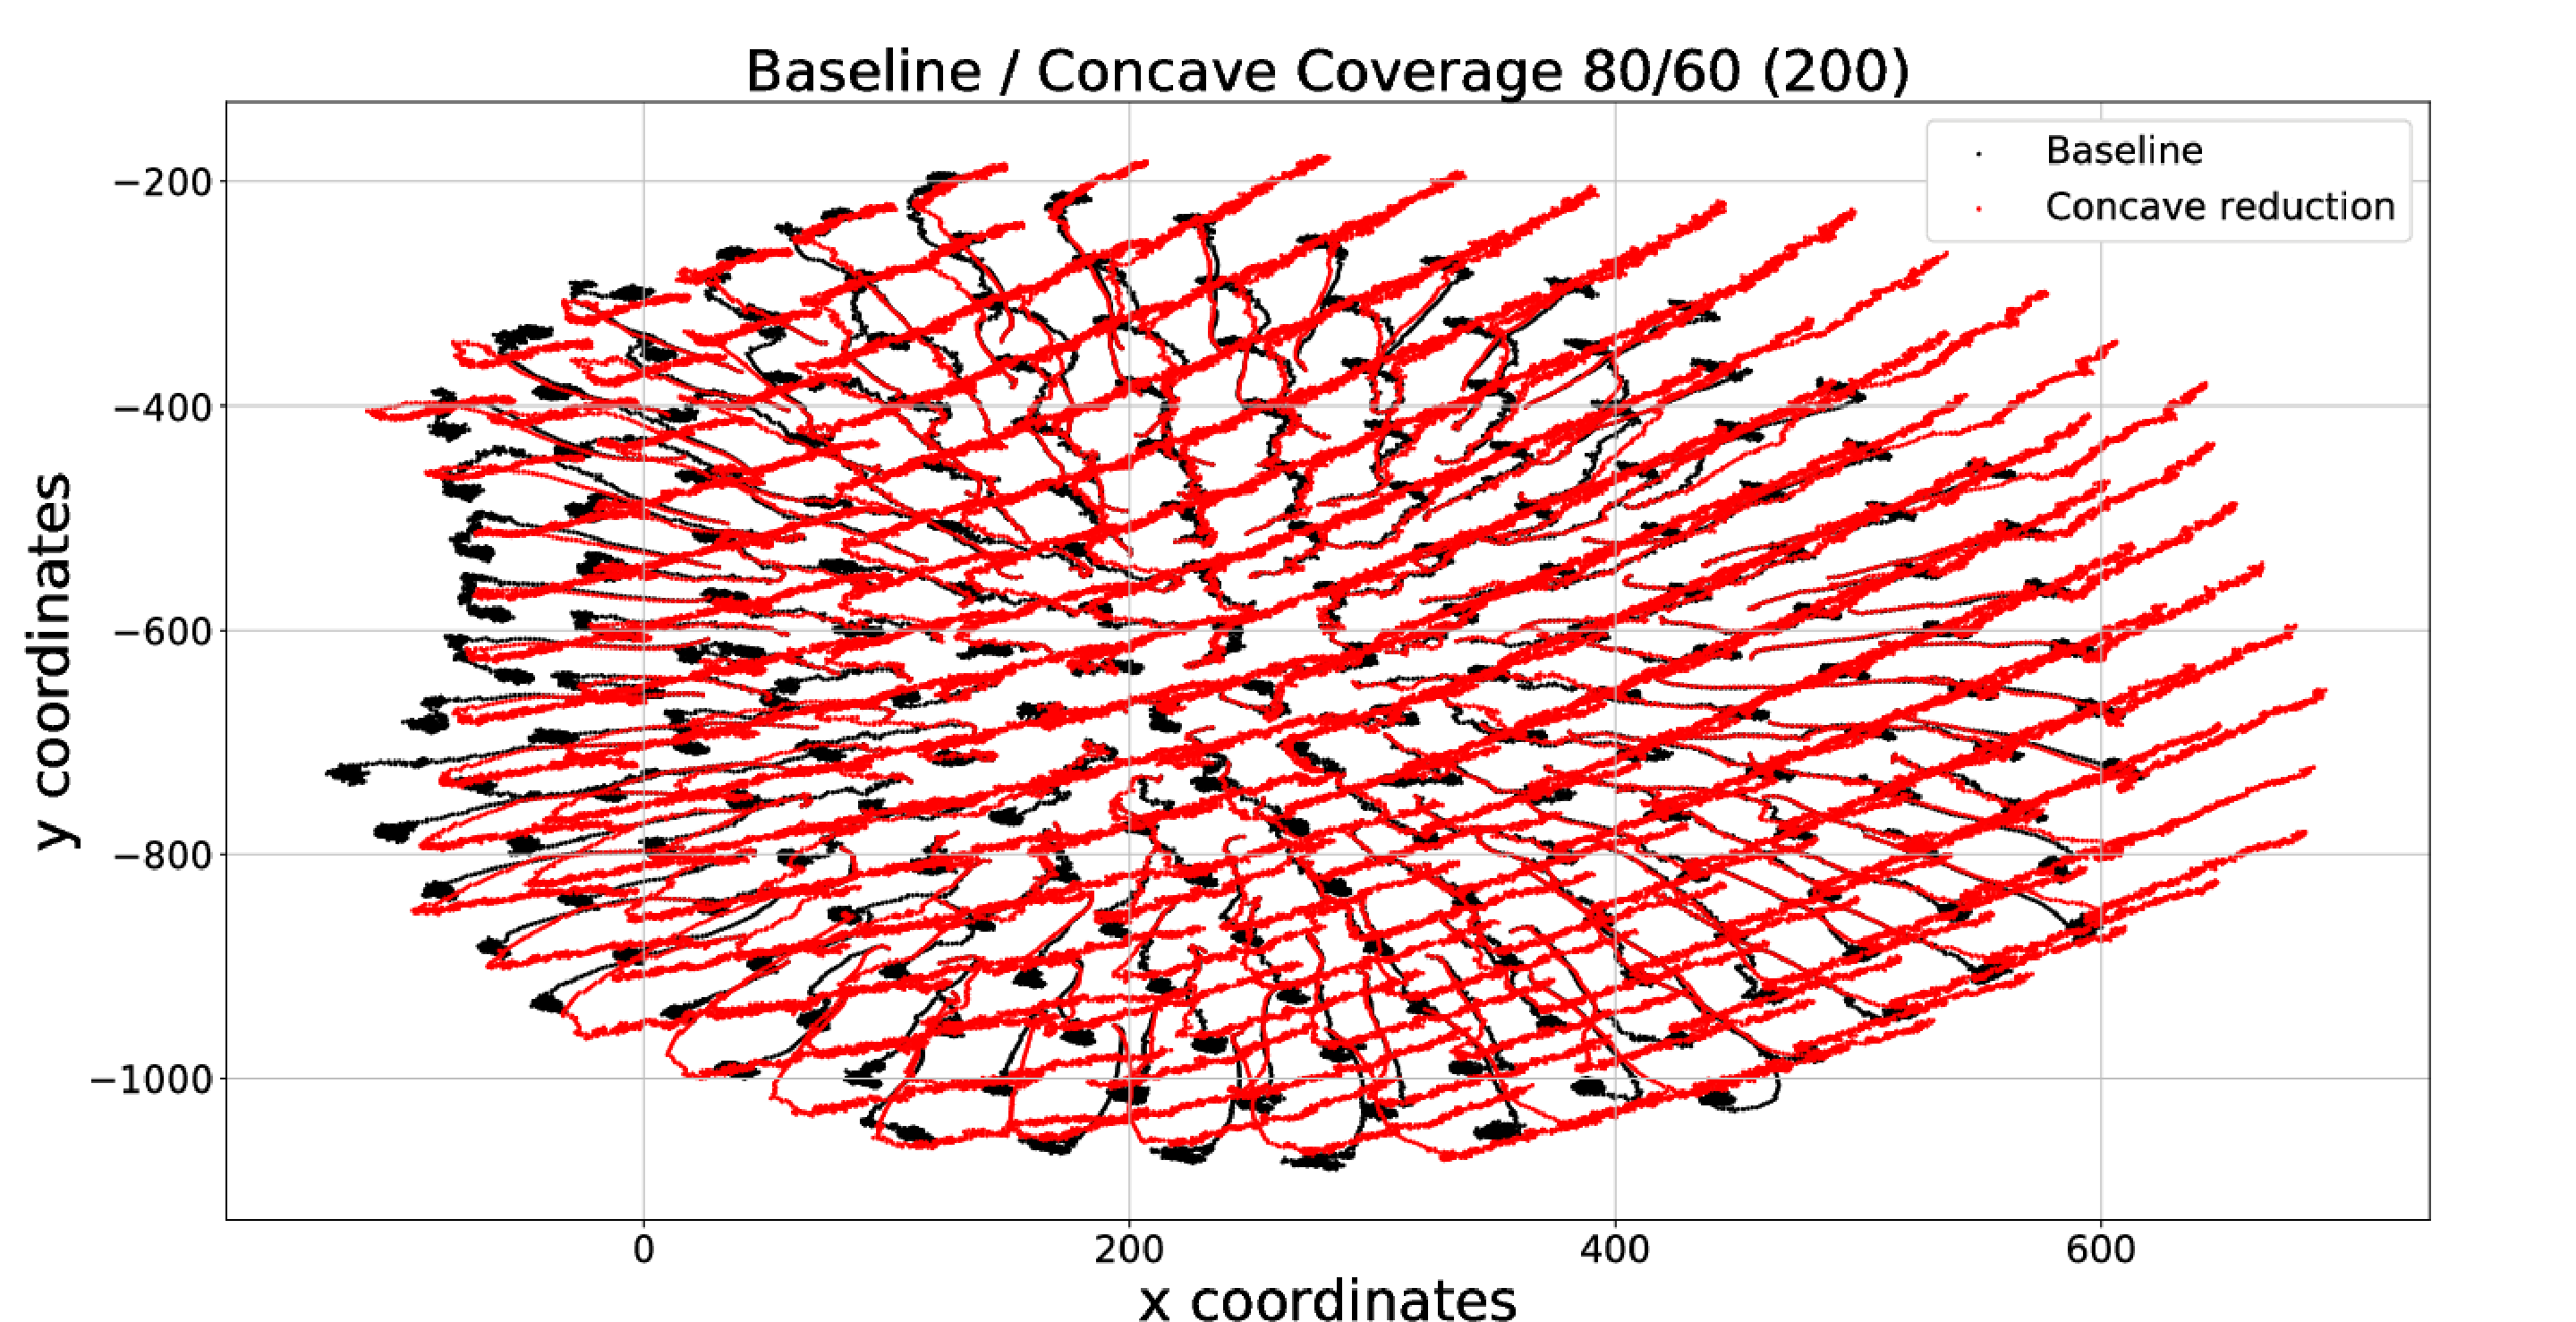
\includegraphics[width=8cm]{figures/BaselineConcaveEffectPath80601}
%% \end{center}
%% \caption{Baseline/Concave path effect (80/60)\label{concave:BaselineConcaveEffectPath80601}}
%% \end{figure}

%COVERBASELINE8060.py
\Figure[t!](topskip=0pt, botskip=0pt, midskip=0pt)[width=8.3cm]{figures/BaselineConcaveEffectPath80602}{Baseline/Concave path effect (80/60)\label{concave:BaselineConcaveEffectPath80602}}
%% \begin{figure}
%% \begin{center}
%% 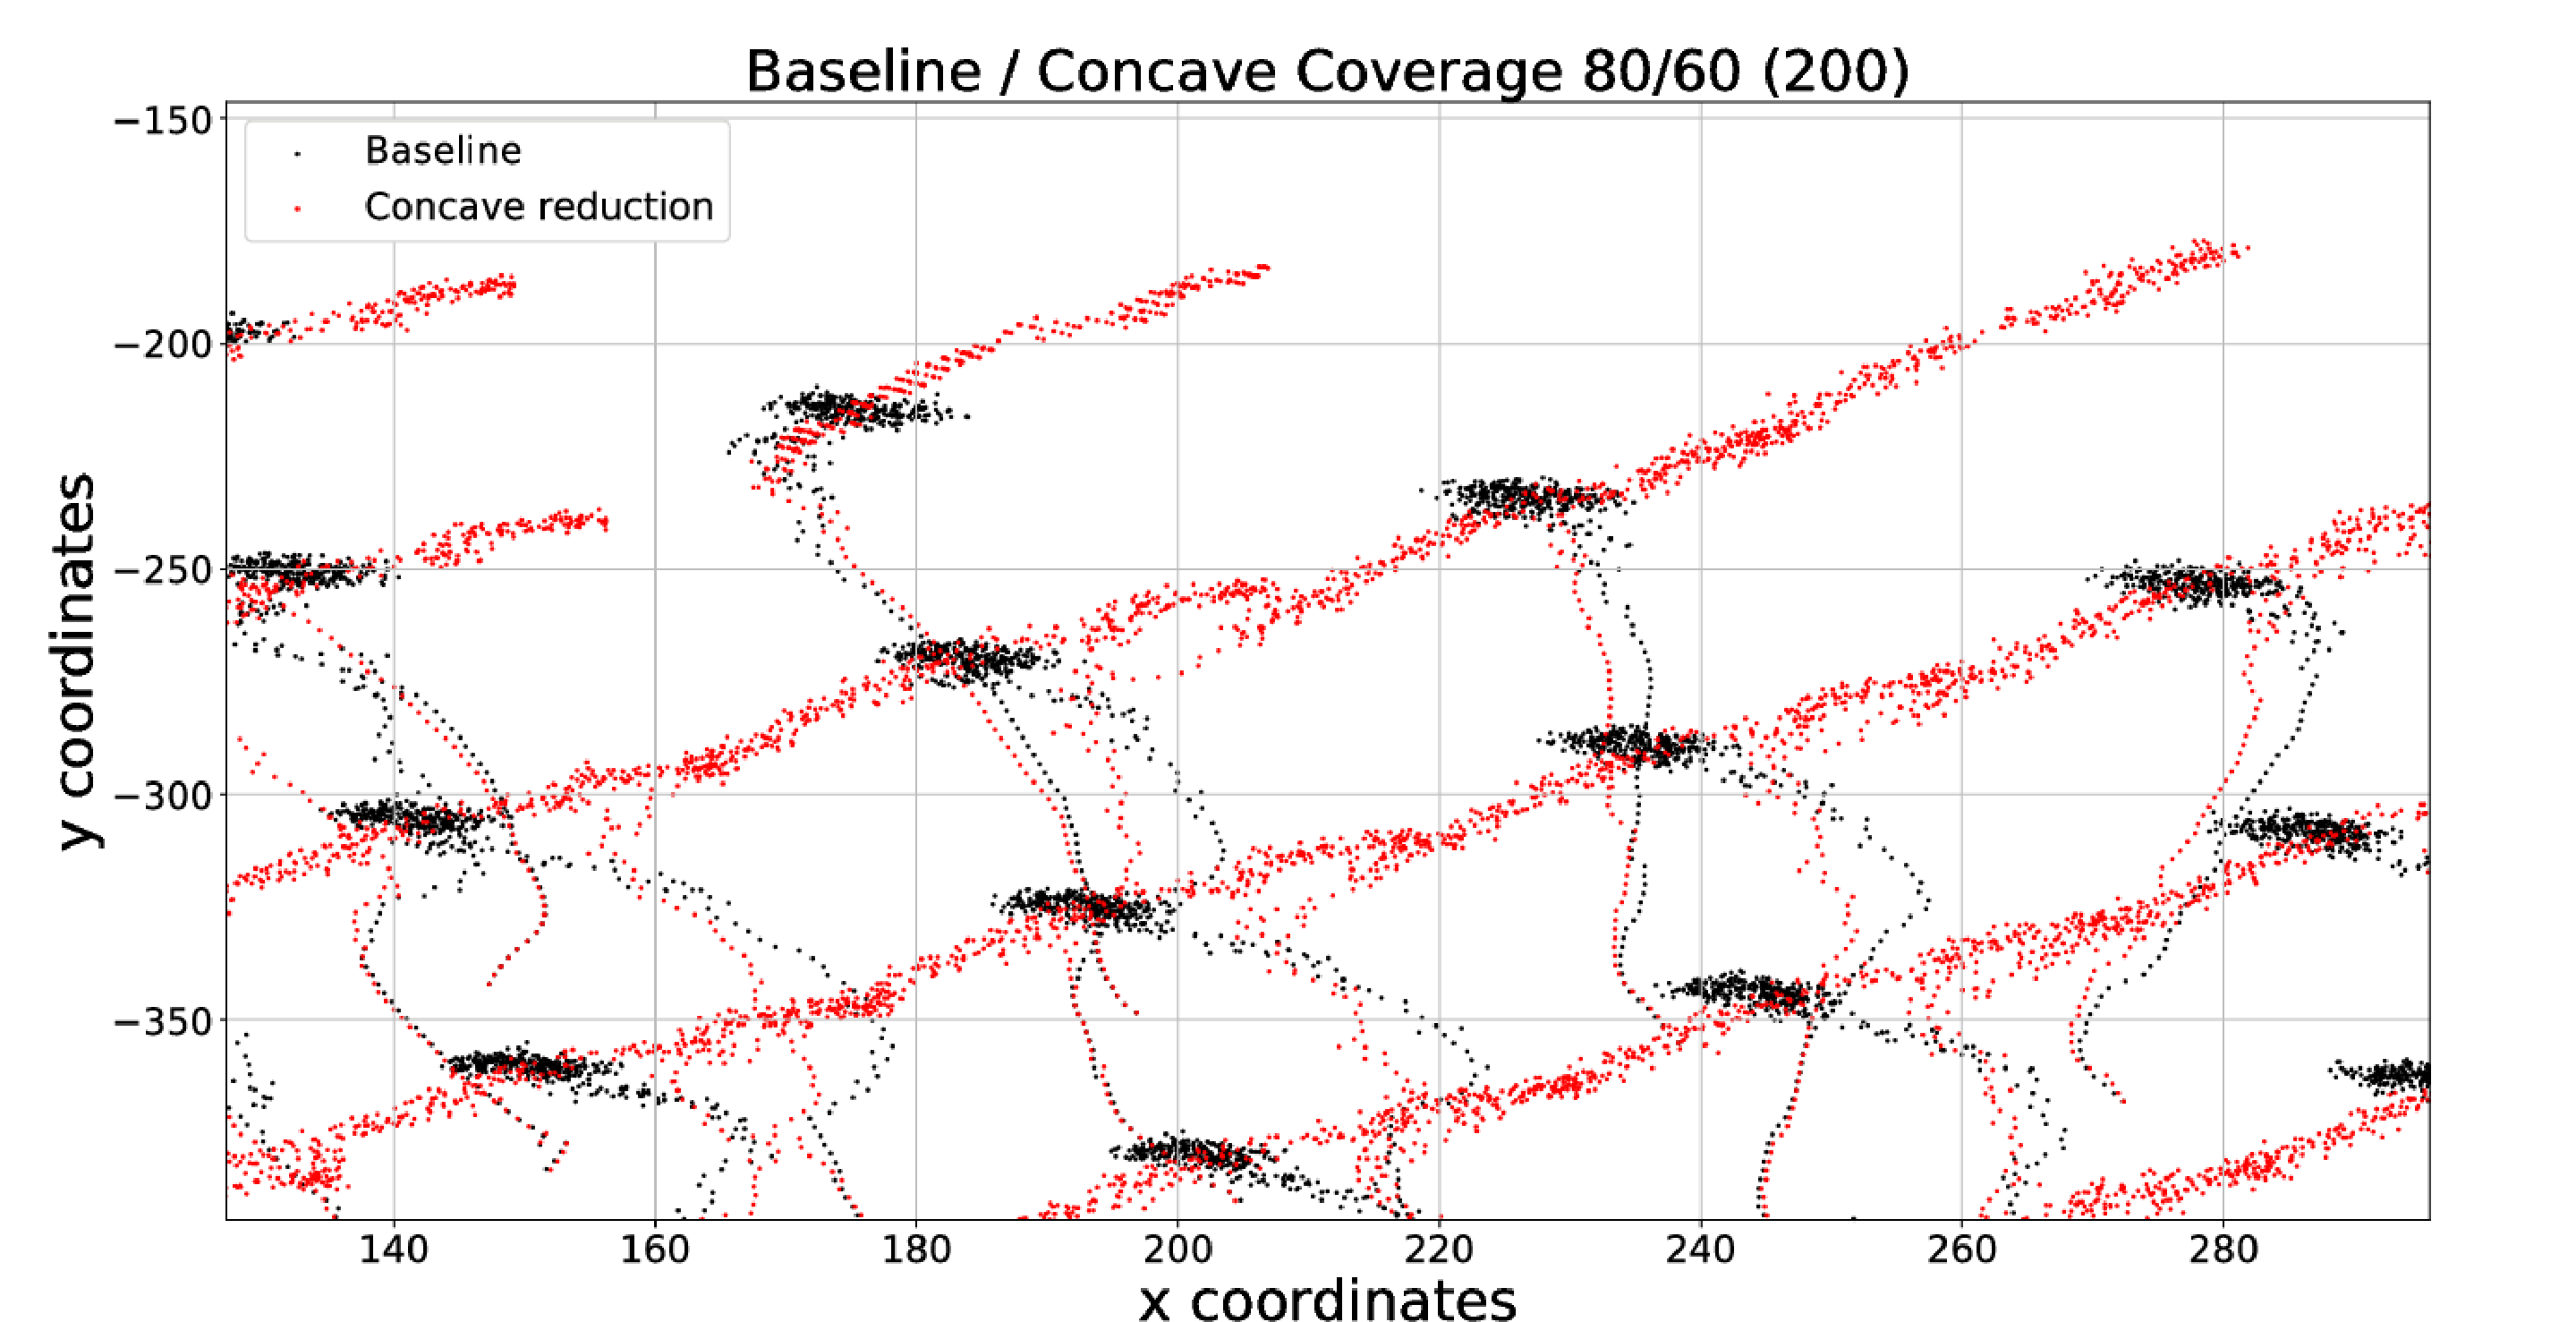
\includegraphics[width=8cm]{figures/BaselineConcaveEffectPath80602}
%% \end{center}
%% \caption{Baseline/Concave path effect (80/60)\label{concave:BaselineConcaveEffectPath80602}}
%% \end{figure}
With the tolerance levels set appropriately the impact of the concave reduction is to reduce the number of agents being identified as coordinators~(Fig.~\ref{concave:mobileSwarm1}). This reduction in perimeter size is due to a reduction in the number of anomalies in the swarm. The effect of the concave reduction on a convex (outer) perimeter is limited when a swarm is deployed in an almost circular manner as there is limited space for optimisation. The effect is more pronounced when a swarm is `malformed' with large anomalies producing concave edges.

\begin{table}
\caption{Comparison of perimeter size} 
\label{tab:BaselineConcaveComparison}
\begin{center}
\begin{tabular}{| p{2.3cm} | p{2cm} | p{2cm} |}
\hline
\bf Neighbour / minimum & \bf Baseline \bf swarm & \bf Concave \bf reduction \\ \hline
80/60 & 19049 & 18940 \\  \hline
80/70 & 27394 & 27987 \\  \hline
\end{tabular}
\end{center}
\end{table}

\section{Application of concave reduction on concave perimeters (voids)}\label{sec:ApplicationConcavePerimeters}
Just as a gap on a convex perimeter is affected by concave reduction so is the perimeter of a concave perimeter (a void). The effect on a concave perimeter is more pronounced due to there being a higher ratio of concave anomalies. It is possible to have no concave gaps on a convex perimeter (a circular swarm) but a concave perimeter (void) always has concave anomalies. This characteristic allows voids to be controlled. To test the effect of concave reduction on void removal a baseline must be established~(Fig.~\ref{tab:BaselineConcaveReduction3}).
As with the previous testing of algorithm effects the comparison needs to take into consideration jitter (inter-agent distance and \textit{inter-agent magnitude}) and the effect on the number of coordinator agents (perimeter agents). 
Table~\ref{tab:BaselineConcaveReduction3} shows the swarm parameters for void removal by concave reduction.

\begin{table}
\caption{Baseline comparison for concave reduction} 
\label{tab:BaselineConcaveReduction3}
\begin{center}
\begin{tabular}{| p{1.4cm} | p{1.2cm} | p{1.2cm} | p{2.5cm} |}
\hline
\bf Weight \bf component & \bf Baseline \bf swarm & \bf Concave \bf reduction & \bf Description \\ \hline
Sample rate & 100 & 100 & ms - Unit sampling interval\\  \hline
$k_{cr}$ & 0 & 100 & weight adjuster for concave reduction vector\\  \hline
$k_c$ & 5 & 5 & weight adjuster for cohesion field\\  \hline
$k_r$ & 15 & 15 & weight adjuster for repulsion field\\  \hline
$k_d$ & 0 & 0 & weight adjuster for destination vector 0 for static baseline 100 from goal-based\\  \hline
Repulsion Boundary & 45 & 45 & units\\  \hline
Neighbour Distance & 60 & 60 & units\\  \hline
Speed & 20 & 20 & units/s\\  \hline
\end{tabular}
\end{center}
\end{table}

Figure~\ref{fig:BaselineEndPoint4560} and \ref{fig:ConcaveEndPoint4560} shows the end points for the simulations for the concave reduction experiments. Figure~\ref{fig:BaselineEndPoint4560} shows the end point for the baseline. It shows that at the end of the simulation the void within the swarm persists. This is due to the distribution of the agents being optimal for the given simulation parameters and the structures within the swarm being `stable'. Figure~\ref{fig:ConcaveEndPoint4560} shows the end point for the simulation with concave reduction enabled using the same swarm and configuration parameters. The concave reduction algorithm has removed the void from the swarm completely and the outer perimeter has been `smoothed'. 

%COVERBASELINE4560-BASEEND.py
\Figure[t!](topskip=0pt, botskip=0pt, midskip=0pt)[width=8.3cm]{figures/Baseline4560End}{Baseline end\label{fig:BaselineEndPoint4560}}
%% \begin{figure}
%% \begin{center}
%% 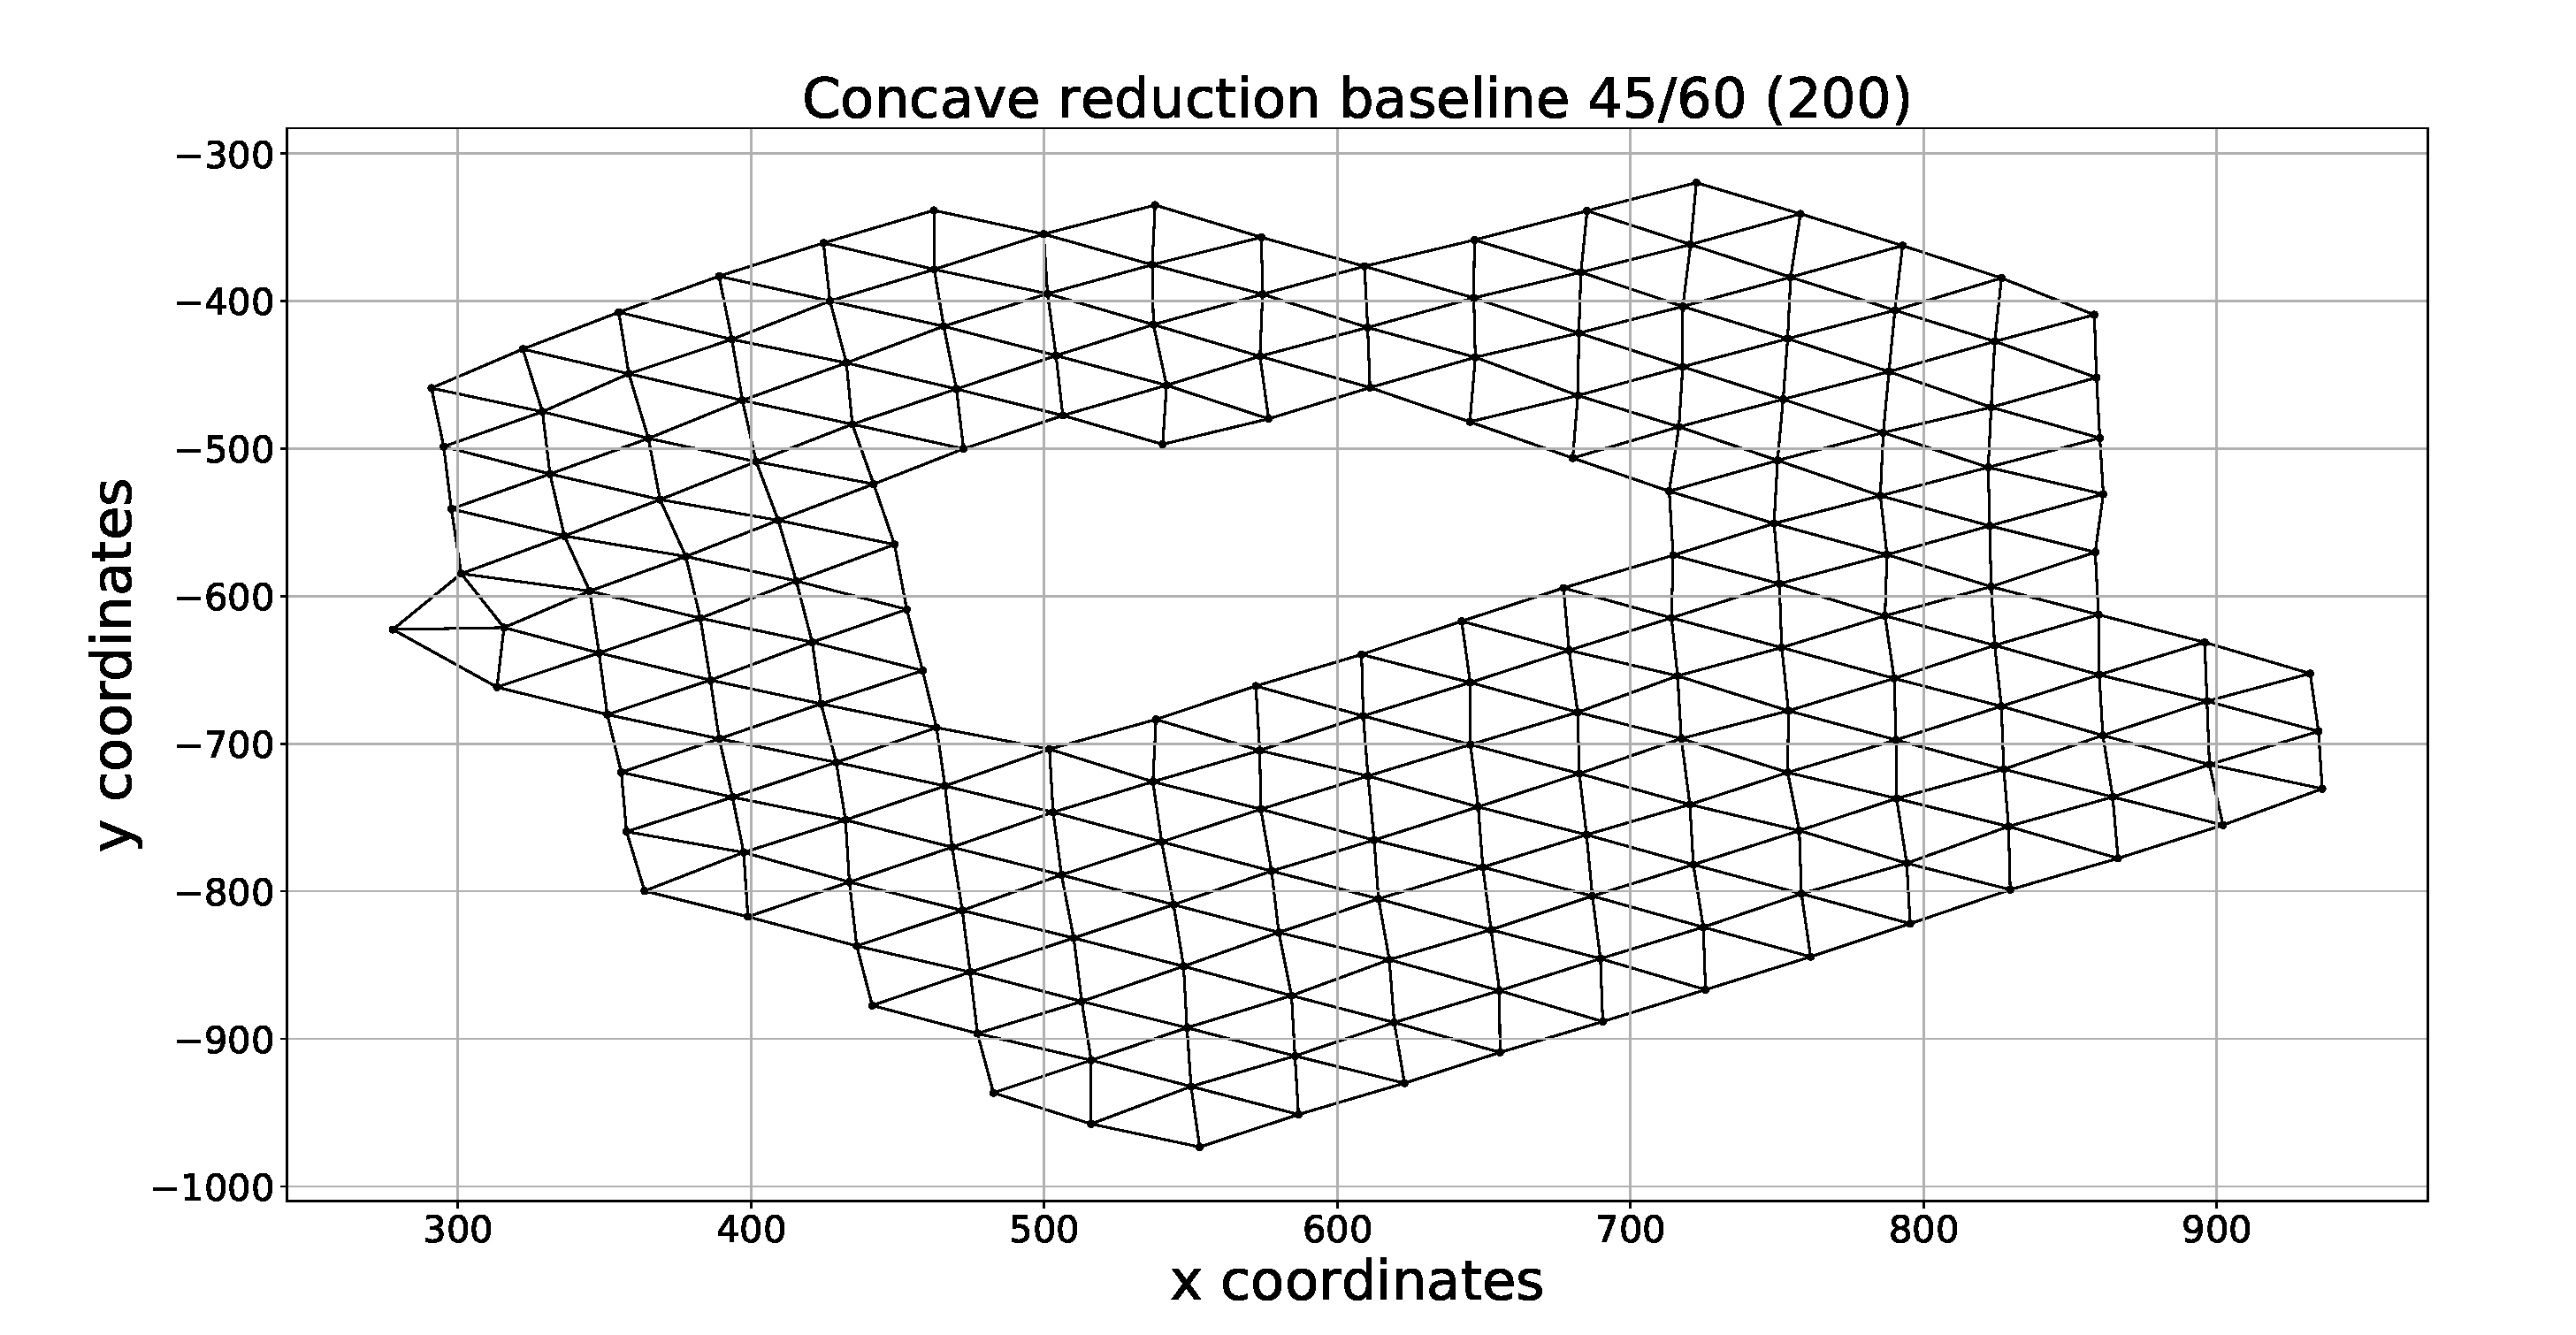
\includegraphics[width=5cm]{figures/Baseline4560End}
%% \end{center}
%% \caption{Baseline end\label{fig:BaselineEndPoint4560}}
%% \end{figure}

%COVERBASELINE4560END3.py
\Figure[t!](topskip=0pt, botskip=0pt, midskip=0pt)[width=8.3cm]{figures/Concave4560End}{Concave end\label{fig:ConcaveEndPoint4560}}
%% \begin{figure}
%% \begin{center}
%% 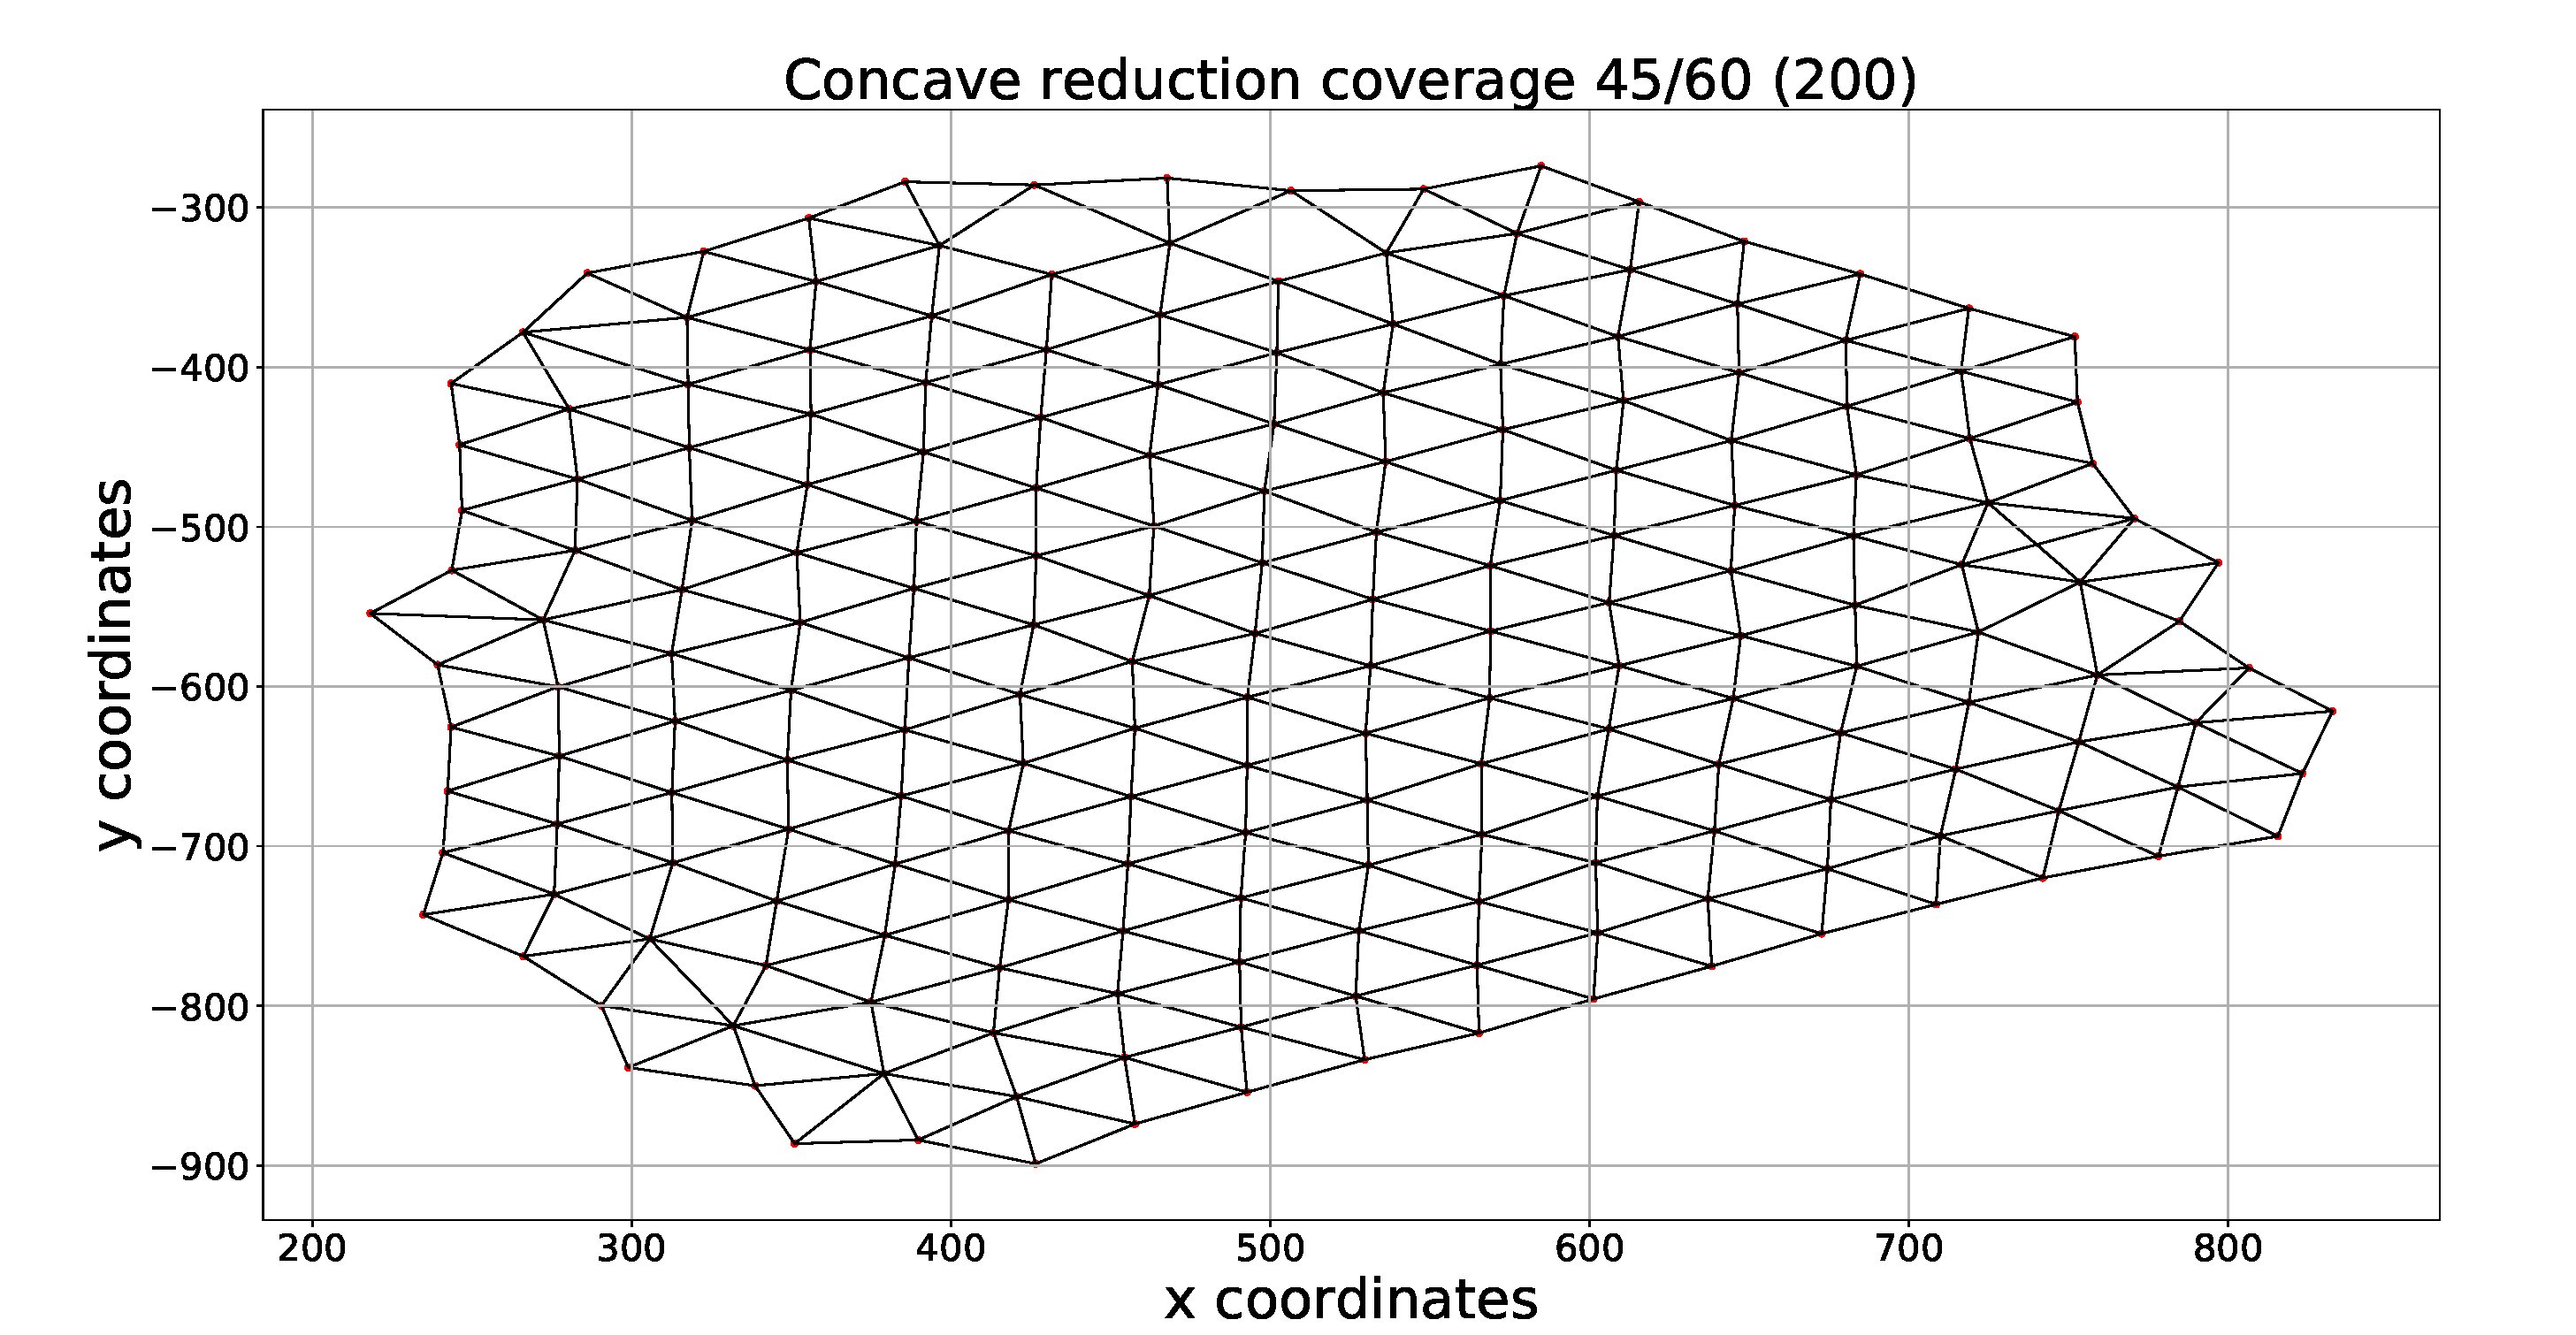
\includegraphics[width=5cm]{figures/Concave4560End}
%% \end{center}
%% \caption{Concave end\label{fig:ConcaveEndPoint4560}}
%% \end{figure}

Figure~\ref{fig:VoidConcaveReduction1}, \ref{fig:VoidConcaveReduction2} and \ref{fig:VoidConcaveReduction3} shows the stages that the swarm goes through when the concave reduction closes the void. The initial deployment of the baseline and concave reduction swarm are the same~(Fig.~\ref{fig:VoidConcaveReduction1}). The concave reduction slowly reduces the void~(Fig.~\ref{fig:VoidConcaveReduction2}) and smooths the outer perimeter. Once the smoothing begins the internal anomaly is filled from behind as the inner agents are drawn into the void. This causes small voids to `percolate' outwards through the swarm until they meet an outer perimeter. Two of these `percolating voids' can be seem in~Fig.~\ref{fig:VoidConcaveReduction2} to the left of the void and above the void. Once the `percolation' process has completed the void is closed~(Fig.~\ref{fig:VoidConcaveReduction3}). The swarm edges also take on a more `rounded' appearance caused by the edges of the swarm being `pulled' to create a convex edge.

%COVERBASELINE4560.py
\Figure[t!](topskip=0pt, botskip=0pt, midskip=0pt)[width=8.3cm]{figures/Concave4560-1}{Initial\label{fig:VoidConcaveReduction1}}
%% \begin{figure}
%% \begin{center}
%% 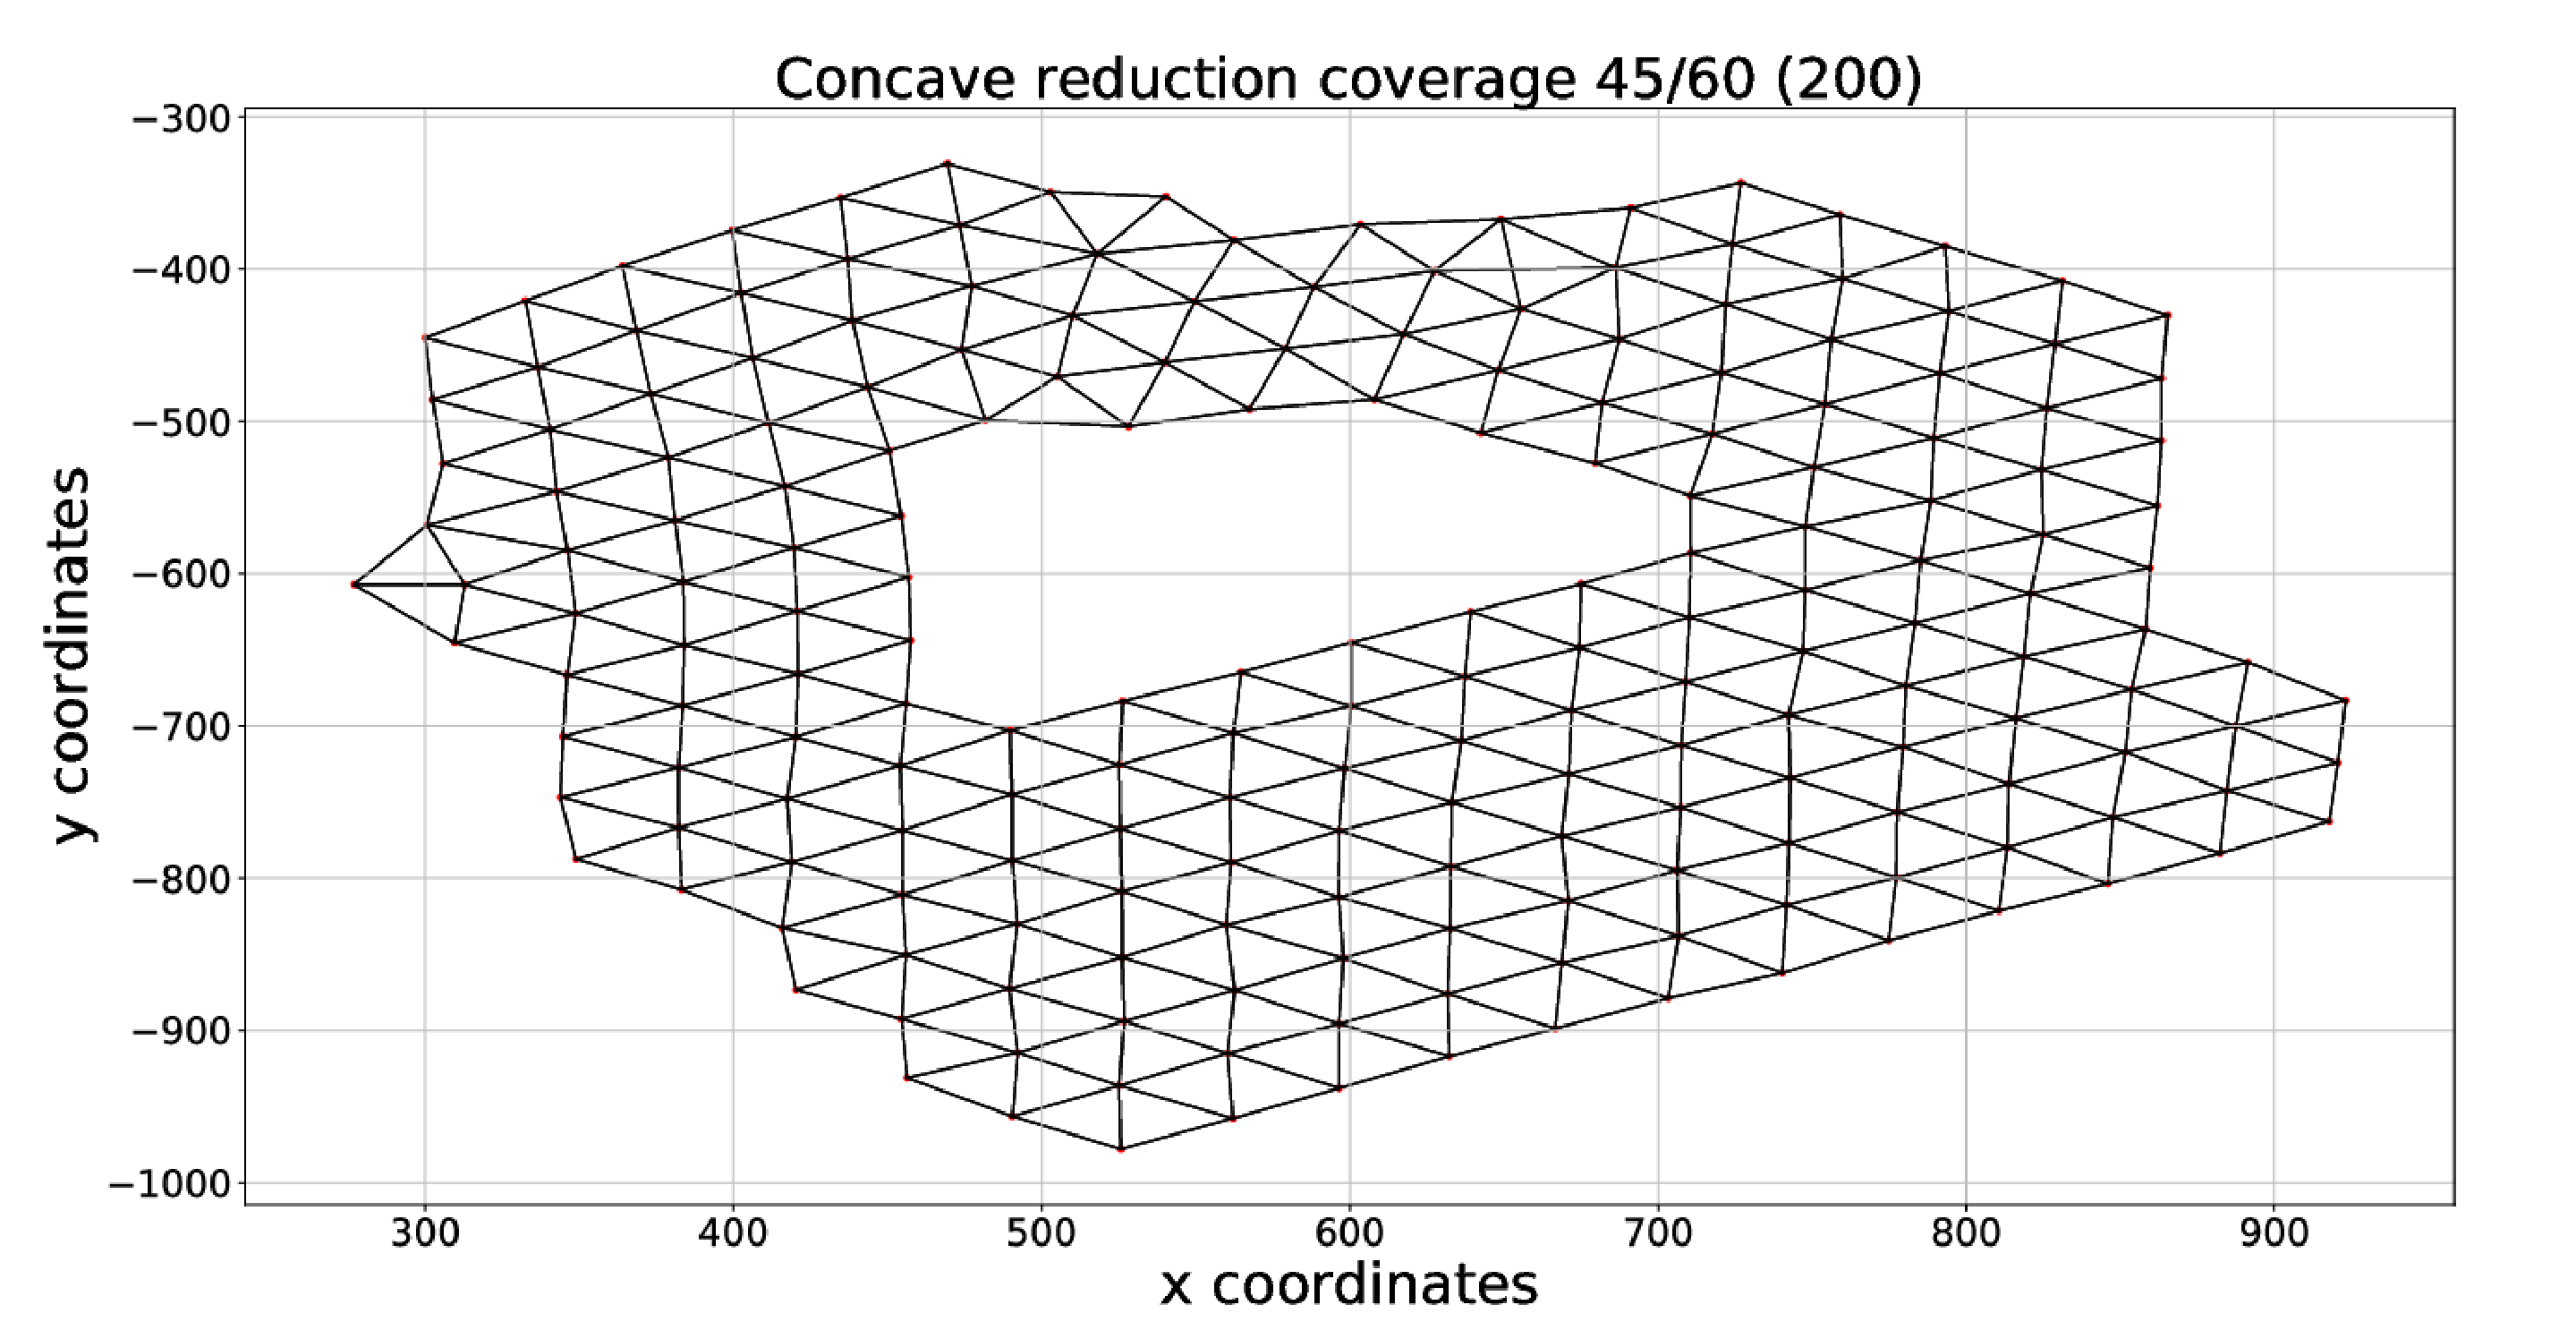
\includegraphics[width=5cm]{figures/Concave4560-1}
%% \end{center}
%% \caption{Initial\label{fig:VoidConcaveReduction1}}
%% \end{figure}

%COVERBASELINE4560END2.py
\Figure[t!](topskip=0pt, botskip=0pt, midskip=0pt)[width=8.3cm]{figures/Concave4560-2}{Partial\label{fig:VoidConcaveReduction2}}
%% \begin{figure}
%% \begin{center}
%% 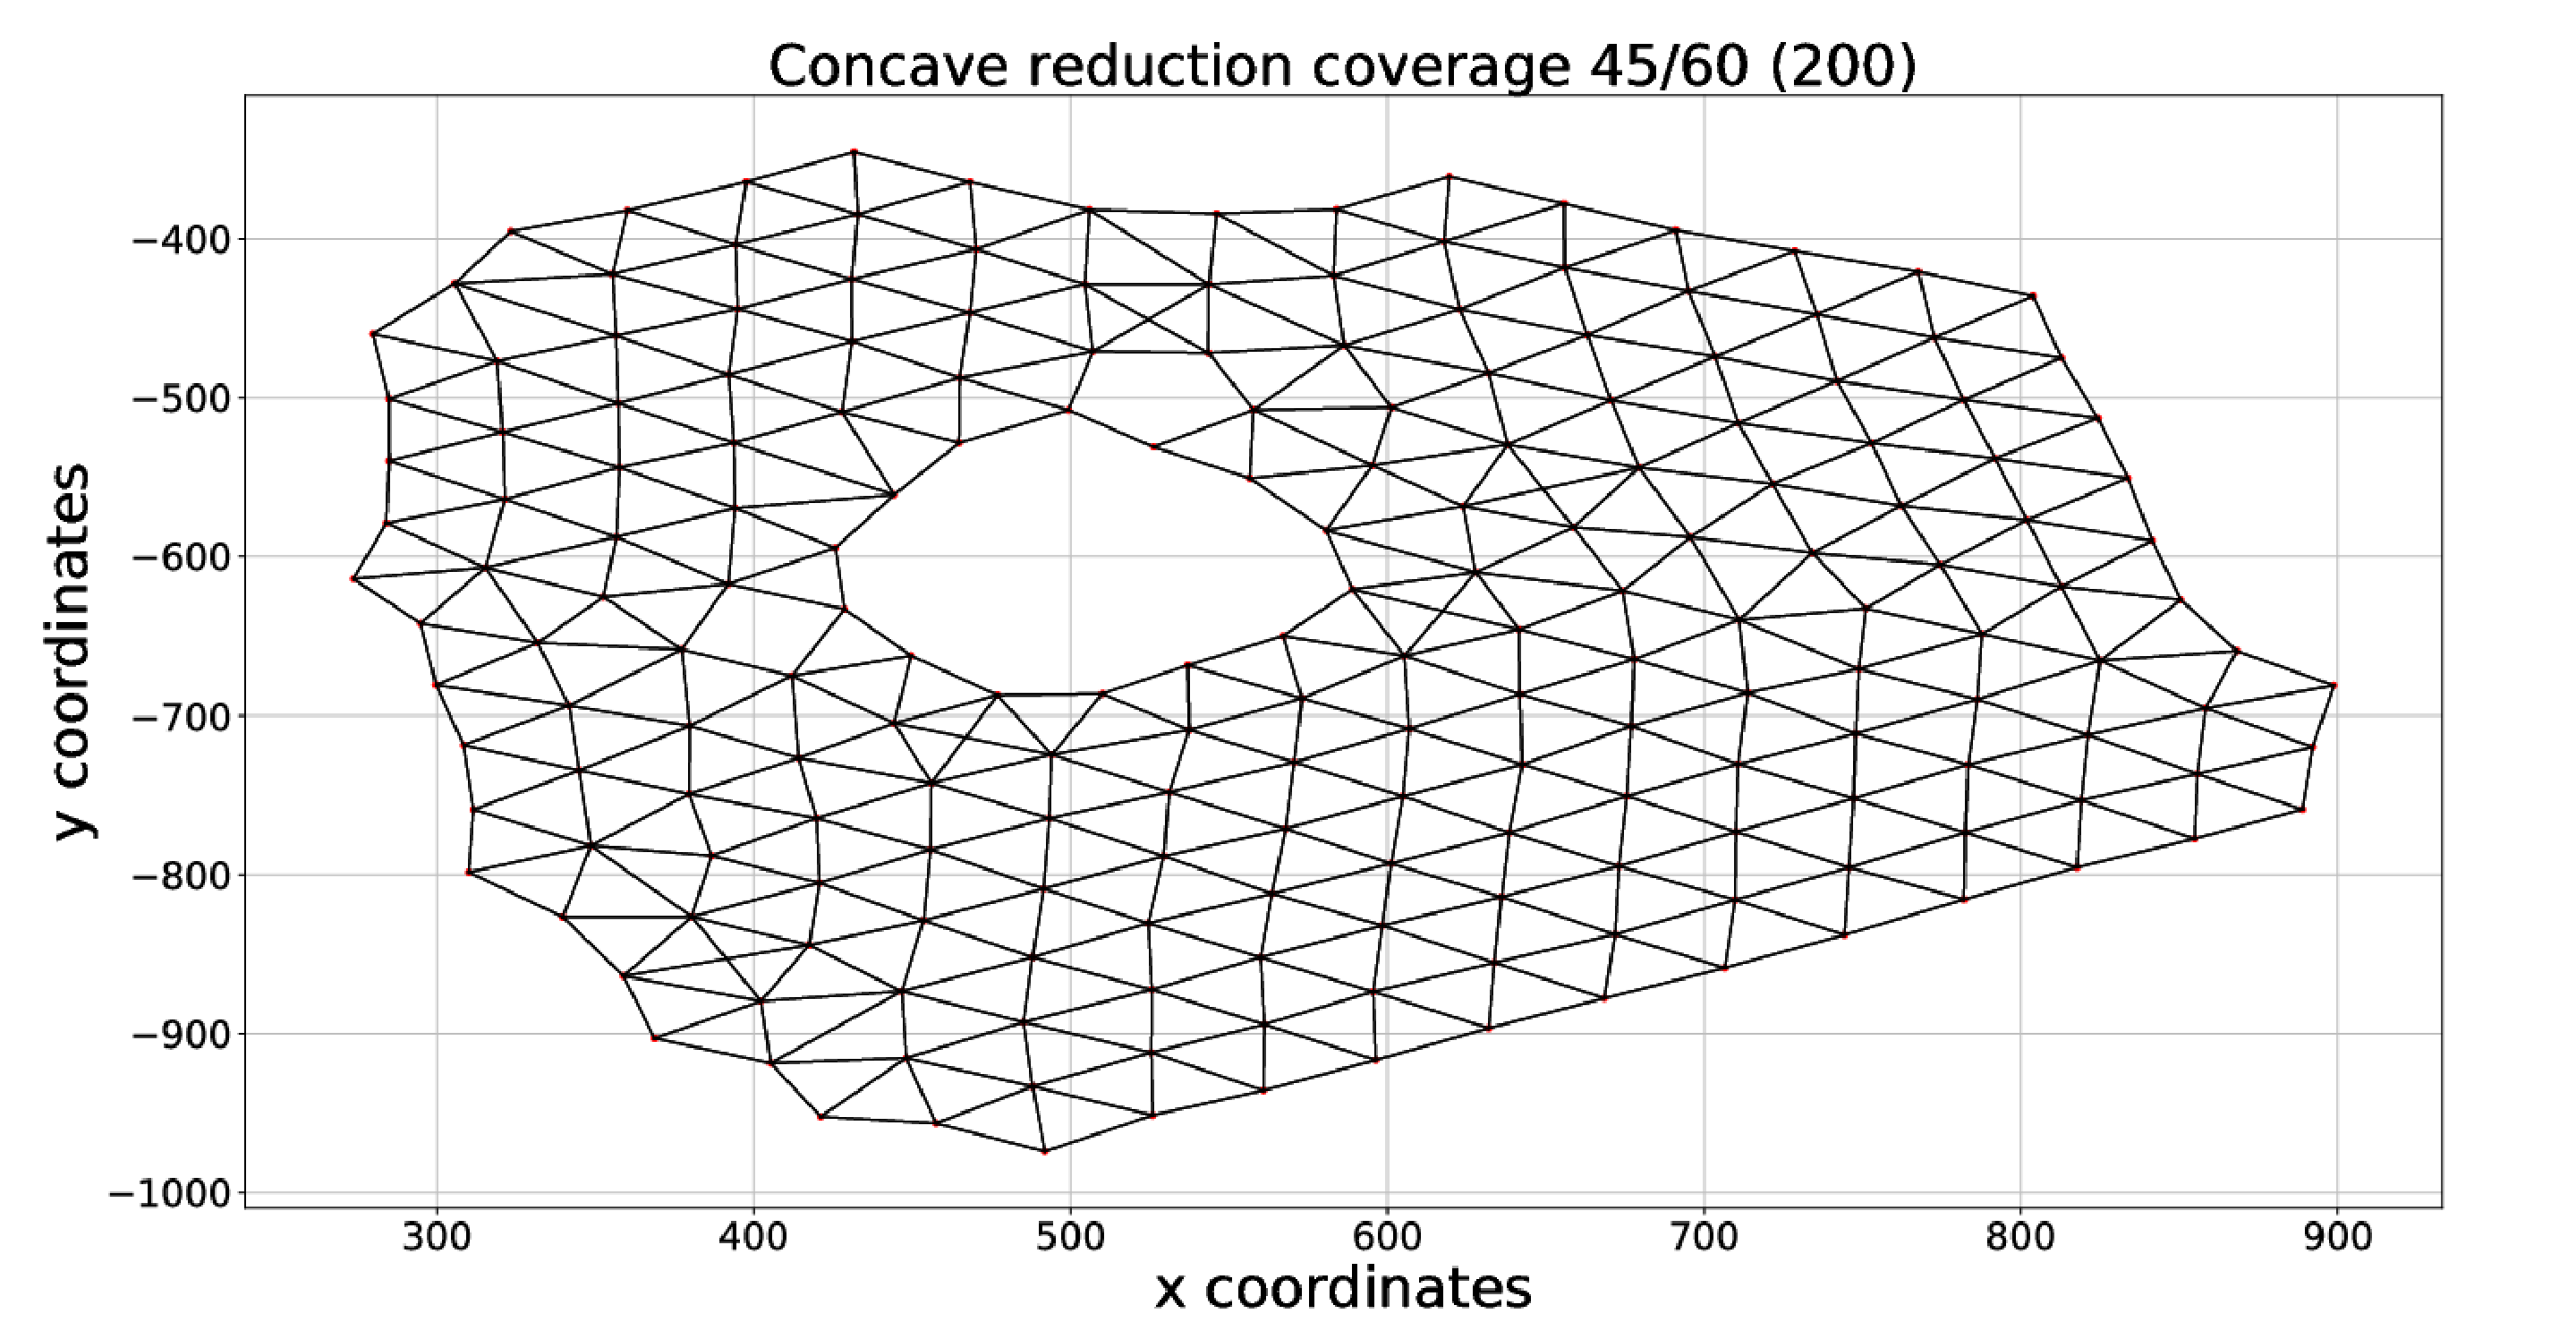
\includegraphics[width=5cm]{figures/Concave4560-2}
%% \end{center}
%% \caption{Partial\label{fig:VoidConcaveReduction2}}
%% \end{figure}

%COVERBASELINE4560END3.py
\Figure[t!](topskip=0pt, botskip=0pt, midskip=0pt)[width=8.3cm]{figures/Concave4560-3}{Complete\label{fig:VoidConcaveReduction3}}
%% \begin{figure}
%% \begin{center}
%% 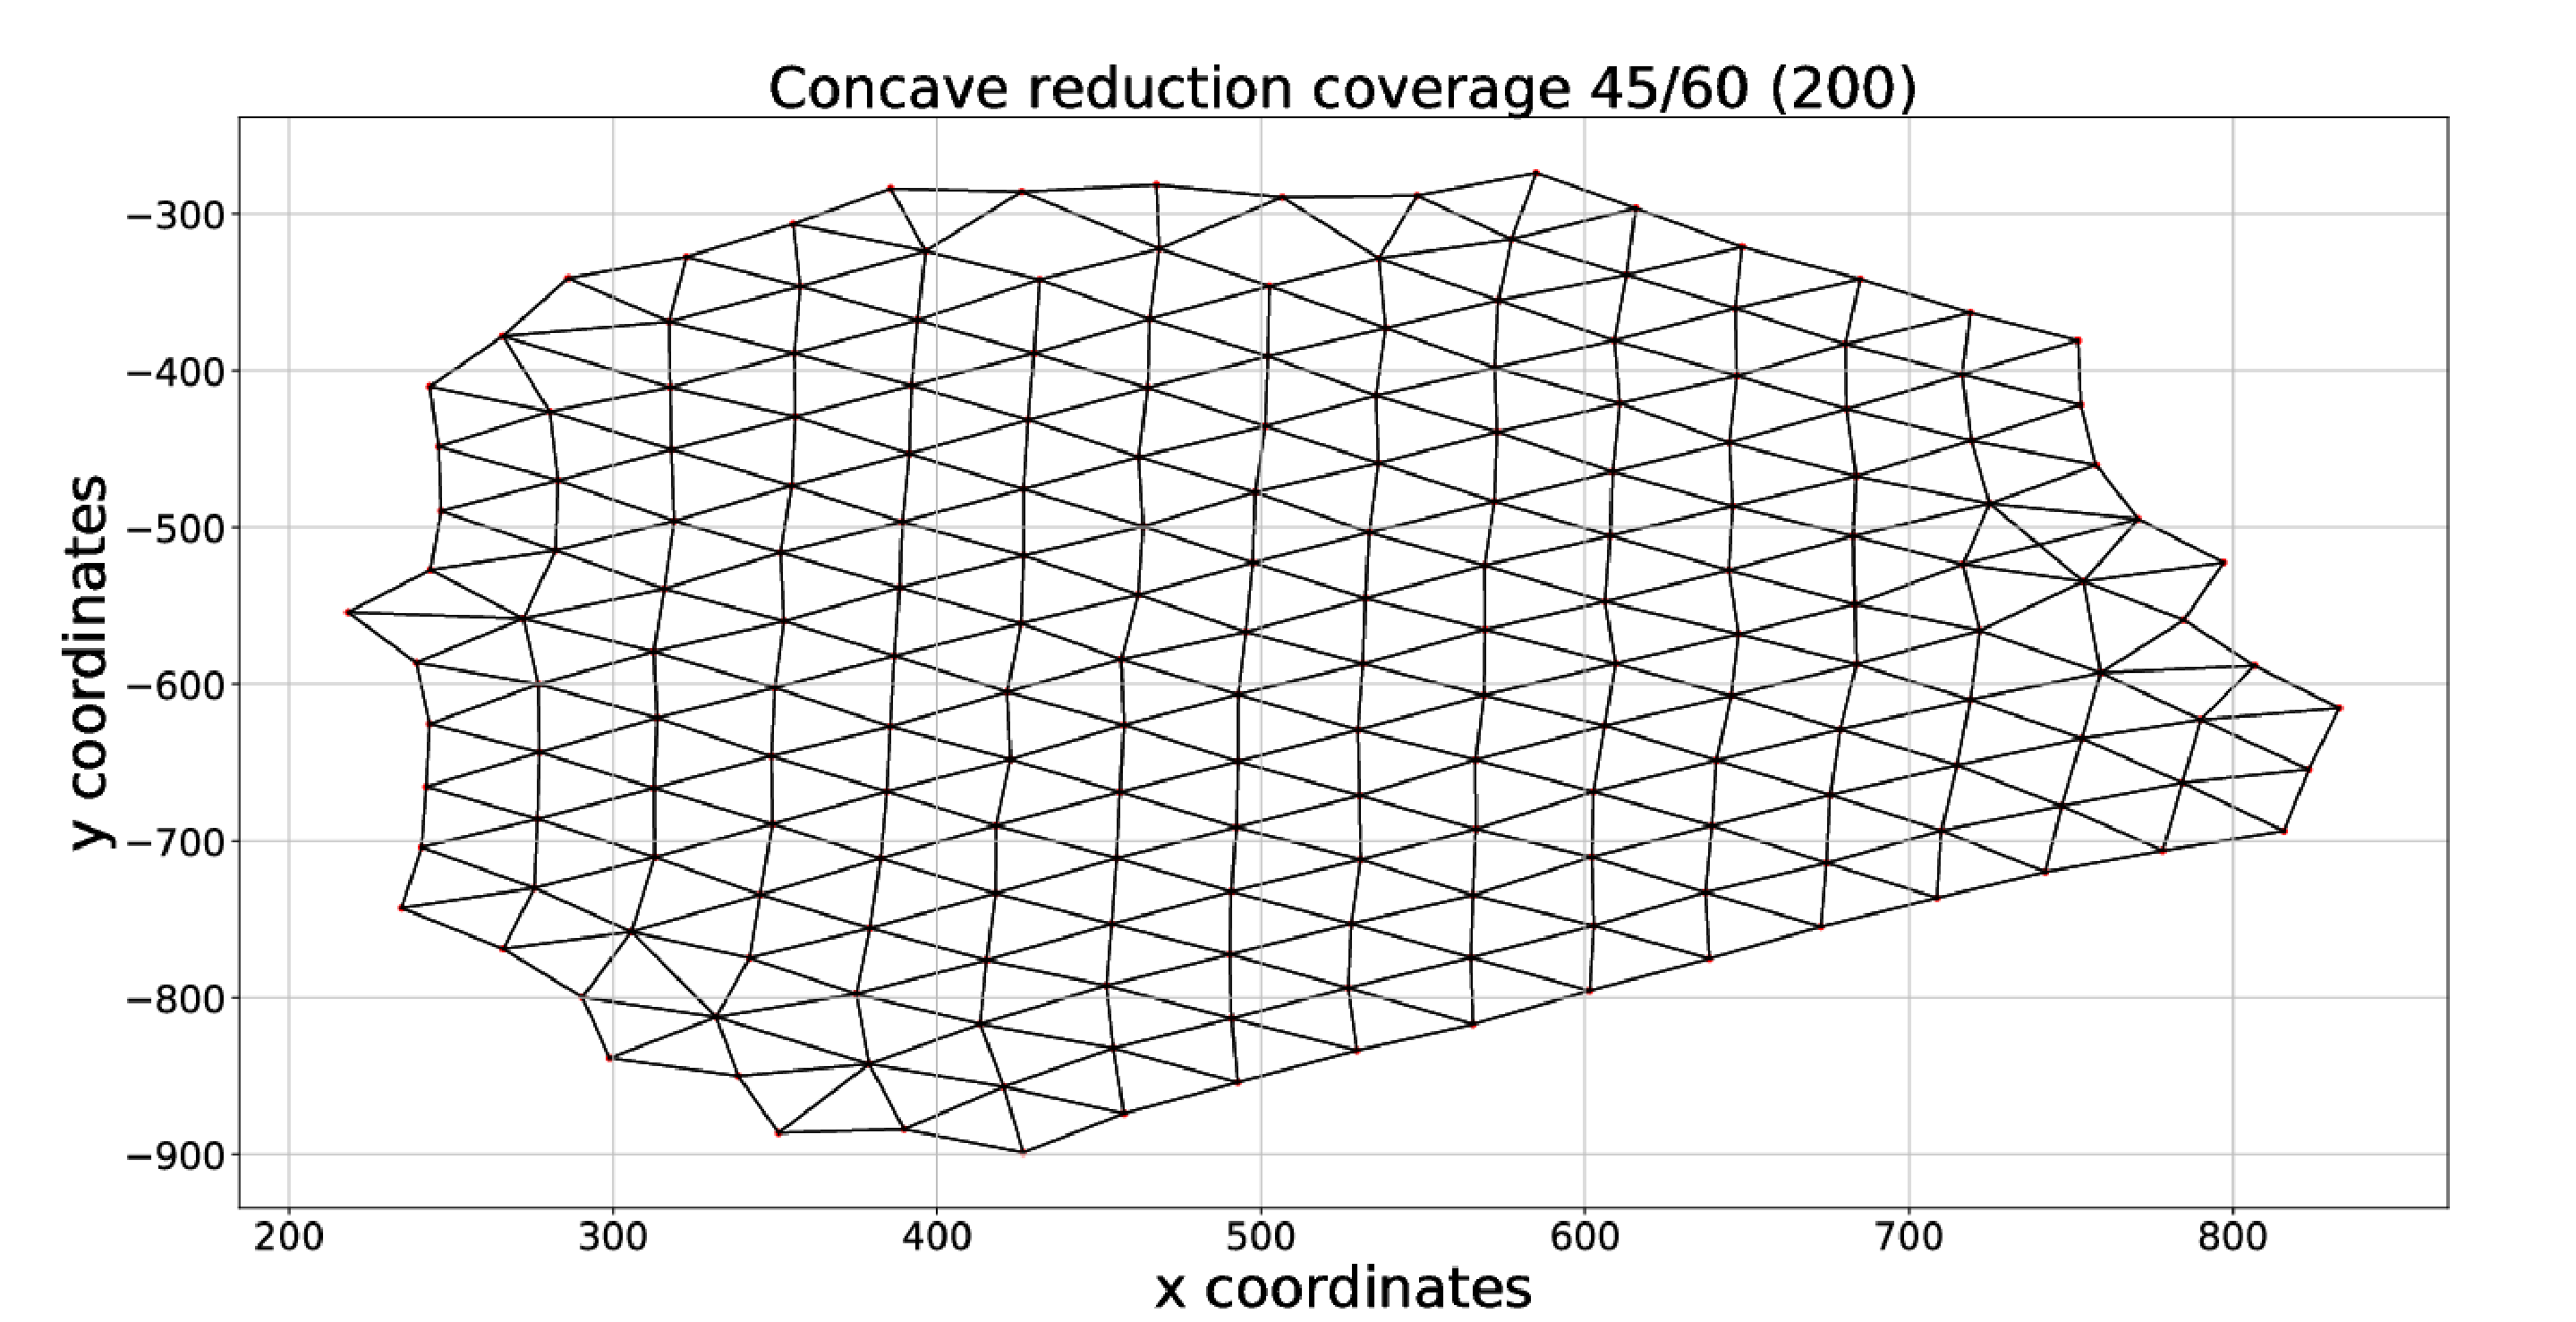
\includegraphics[width=5cm]{figures/Concave4560-3}
%% \end{center}
%% \caption{Complete\label{fig:VoidConcaveReduction3}}
%% \end{figure}

Figure~\ref{voids:ConcavePerimeter4560-DIST}, \ref{voids:ConcavePerimeter4560-DIST-2}, \ref{voids:ConcavePerimeter4560-MAG}, \ref{voids:ConcavePerimeter4560-MAG-2} show the effect the concave reduction has on the inter-agent distances and \textit{inter-agent vector magnitudes} for the simulation. 
Figure~\ref{voids:ConcavePerimeter4560-DIST} shows that the process of reducing the void increases the average distance of the agents. This is caused by the concave agents `pulling' away from their neighbours. The baseline experiment shows a limited change in the variance (jitter) due to the swarm being close to stable even though there is a void present. 
The concave reduction algorithm creates a more pronounced variation due to the void having multiple anomalies. The concave reduction process closes the void over a period of 3 seconds and the swarm then settles to a steady average distance with a stable variance. The increased variance up to 3 seconds is the `percolation' of the internal anomalies to the outer perimeter as the void is closed.

%SWARMHOLE-DIST-4560.py
\Figure[t!](topskip=0pt, botskip=0pt, midskip=0pt)[width=8.3cm]{figures/ConcavePerimeter4560-DIST}{Concave reduction stability effect distance\label{voids:ConcavePerimeter4560-DIST}}
%% \begin{figure}
%% \begin{center}
%% 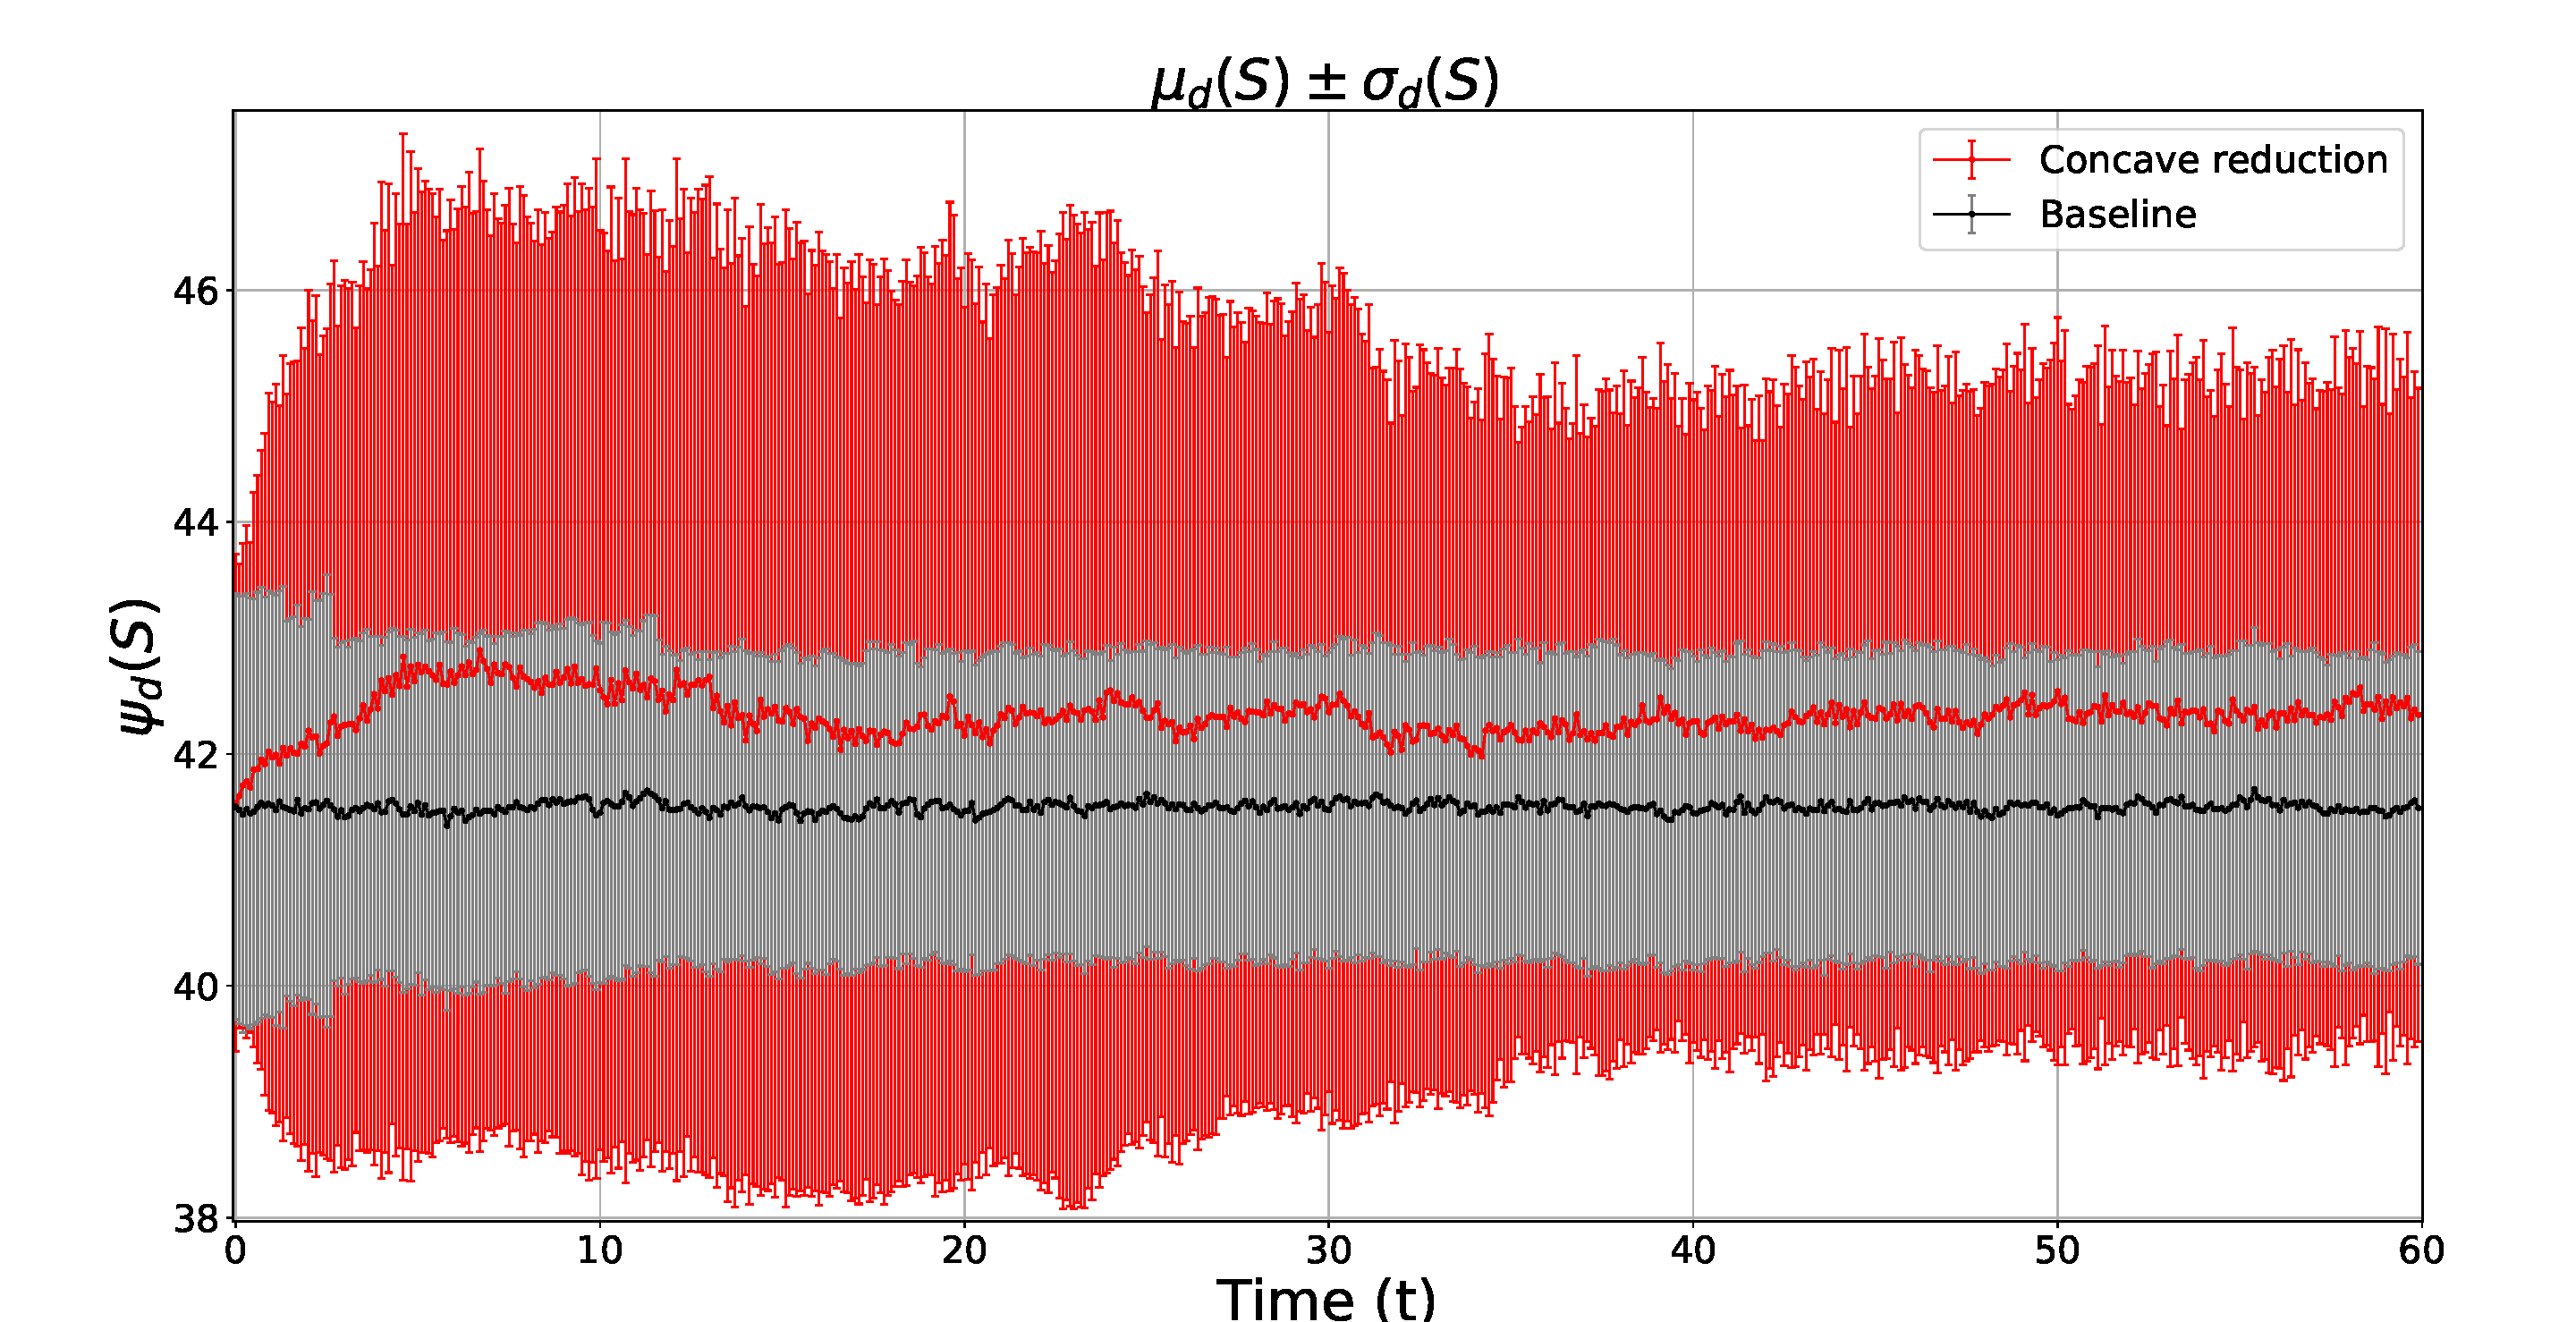
\includegraphics[width=8cm]{figures/ConcavePerimeter4560-DIST}
%% \end{center}
%% \caption{Concave reduction stability effect distance\label{voids:ConcavePerimeter4560-DIST}}
%% \end{figure}

The residual jitter from 3.5 seconds on-wards~(Fig.~\ref{voids:ConcavePerimeter4560-DIST-2}) is the algorithm's effect on the outer perimeter of the swarm. The baseline shows a steadier average with a reduced variance as the basic swarming algorithm allows the agents to settle to a formation that is more structurally stable.

%SWARMHOLE-DIST-4560.py
\Figure[t!](topskip=0pt, botskip=0pt, midskip=0pt)[width=8.3cm]{figures/ConcavePerimeter4560-DIST-2}{Concave reduction stability effect distance\label{voids:ConcavePerimeter4560-DIST-2}}
%% \begin{figure}
%% \begin{center}
%% 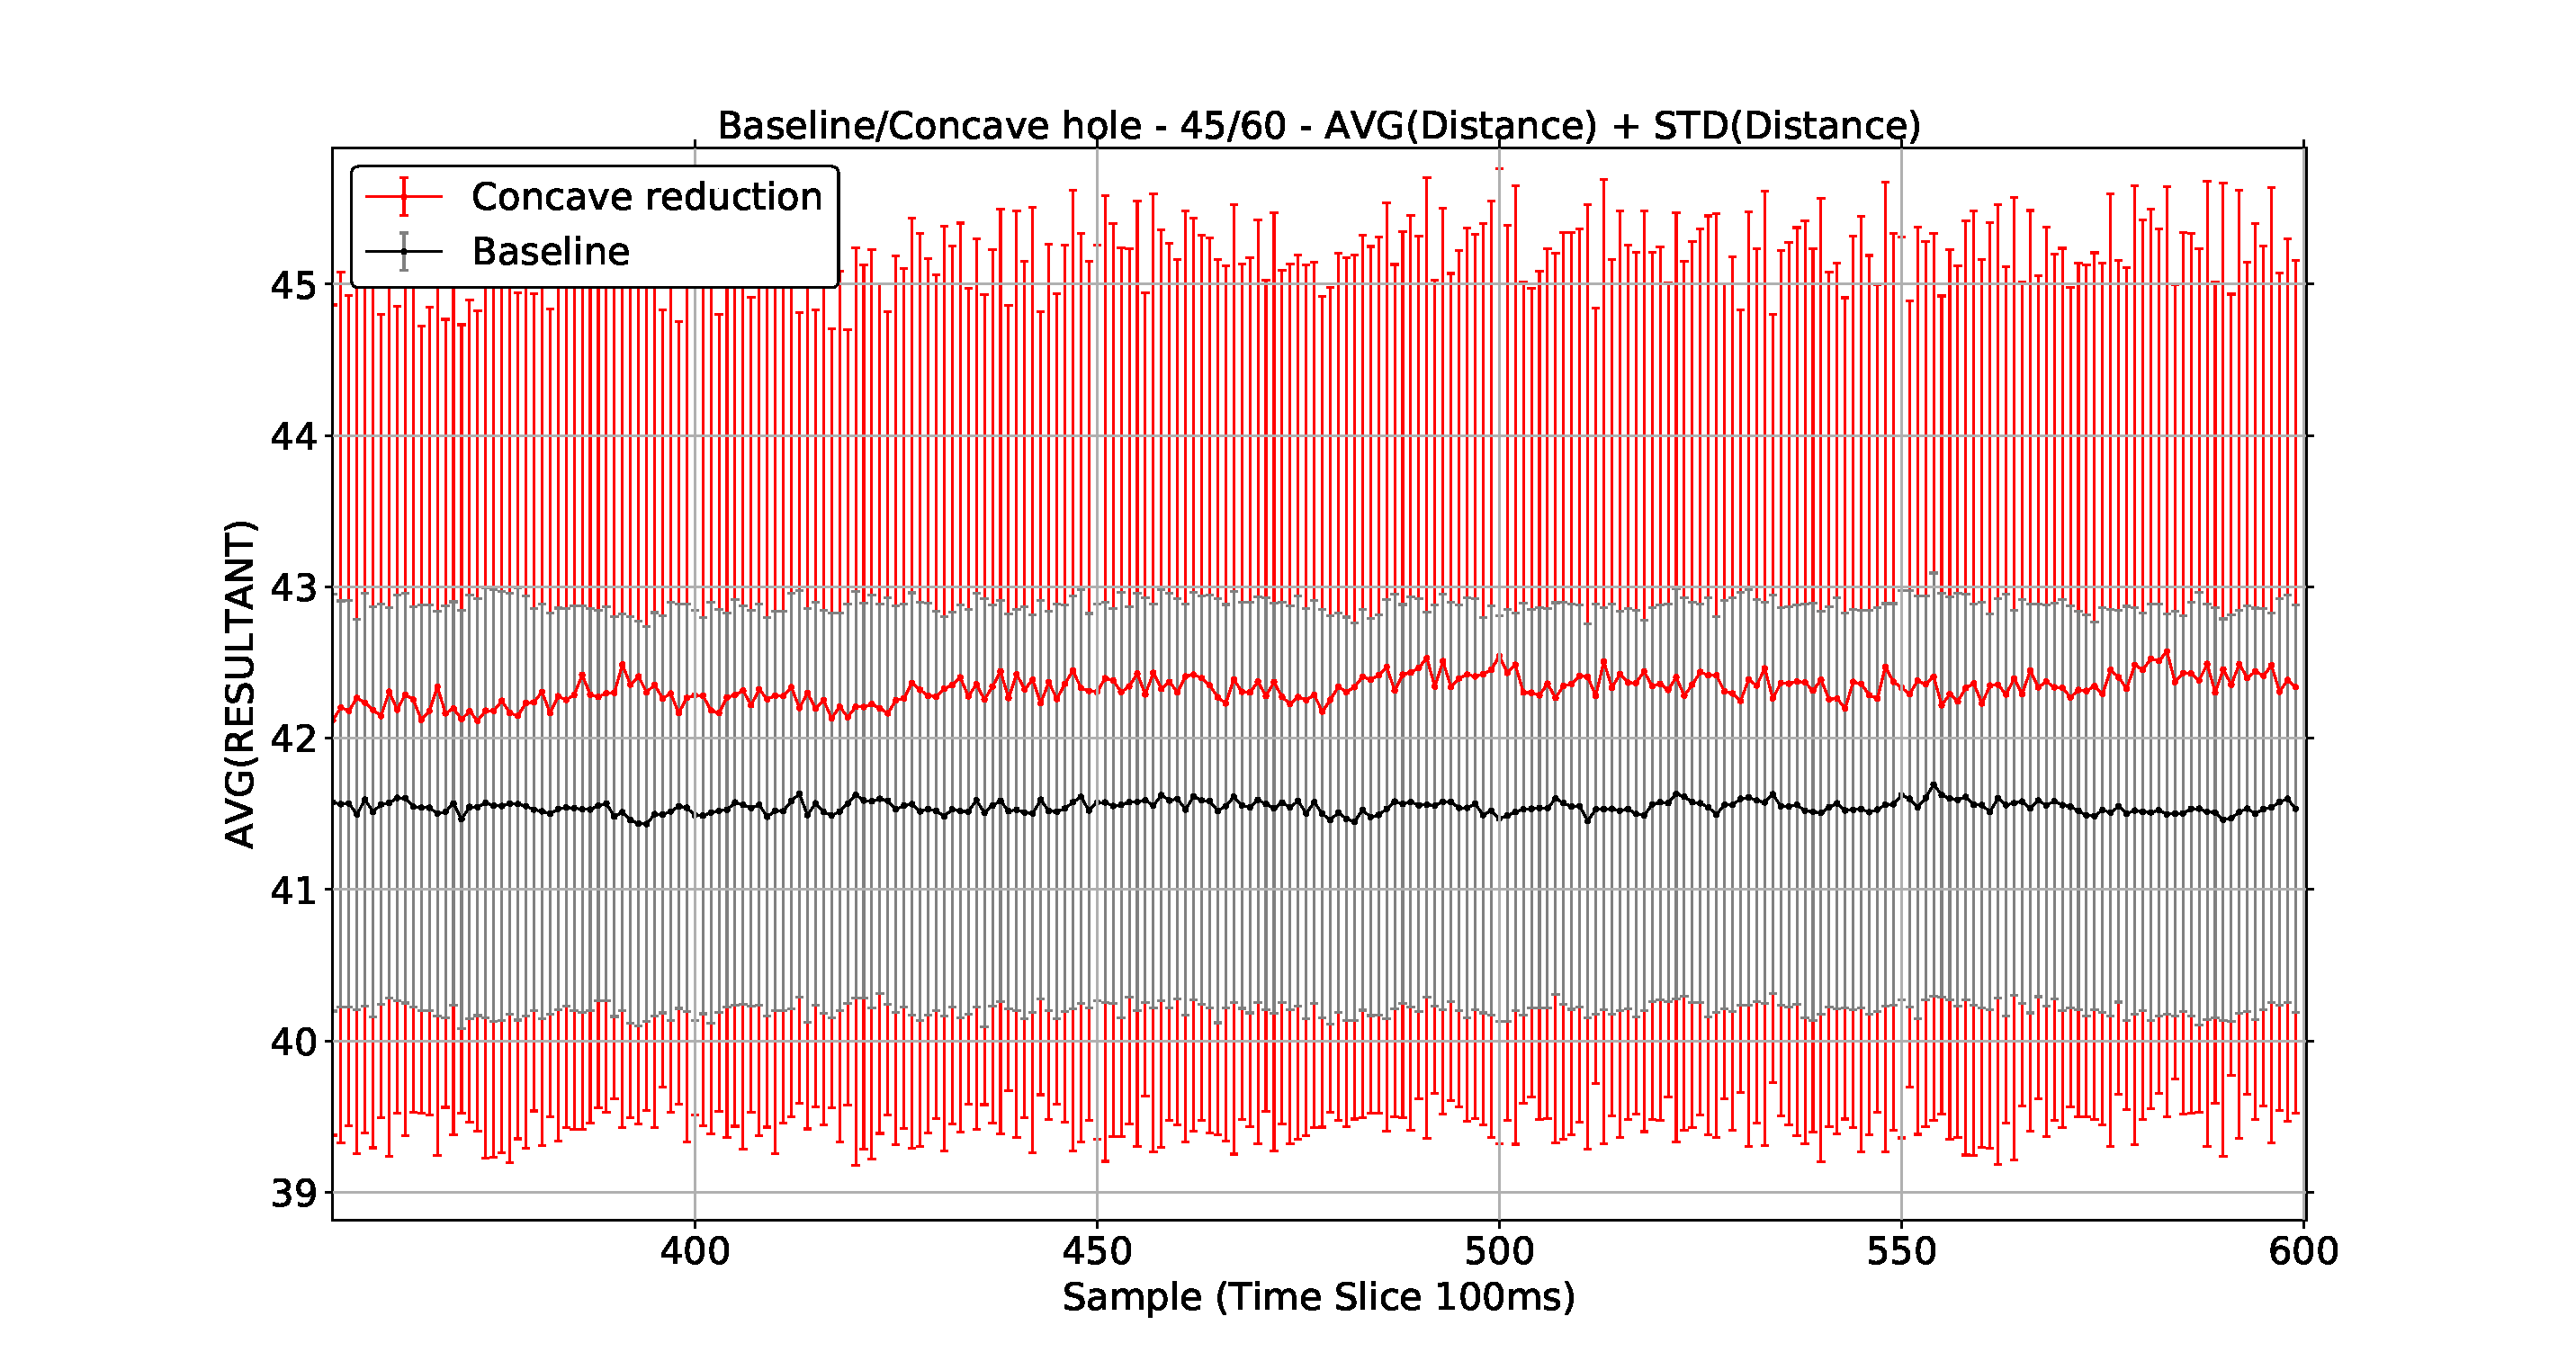
\includegraphics[width=8cm]{figures/ConcavePerimeter4560-DIST-2}
%% \end{center}
%% \caption{Concave reduction stability effect distance\label{voids:ConcavePerimeter4560-DIST-2}}
%% \end{figure}
Figure~\ref{voids:ConcavePerimeter4560-MAG} shows that although the algorithm has introduced jitter and therefore increased both the average \textit{inter-agent magnitude} and the variance the resultant changes have not caused the swarm to become cohesively unstable. The magnitude and the variance never take the magnitude below 0. From 3.5 seconds the \textit{inter-agent magnitude} fluctuates slightly with an increased variance caused by the re-positioning of the concave agents. Although the agents are less structured the increased resultant magnitude ensures the swarm remains cohesive. 
%SWARMHOLE-MAG-4560.py
\Figure[t!](topskip=0pt, botskip=0pt, midskip=0pt)[width=8.3cm]{figures/ConcavePerimeter4560-MAG}{Concave reduction stability effect magnitude\label{voids:ConcavePerimeter4560-MAG}}
%% \begin{figure}
%% \begin{center}
%% 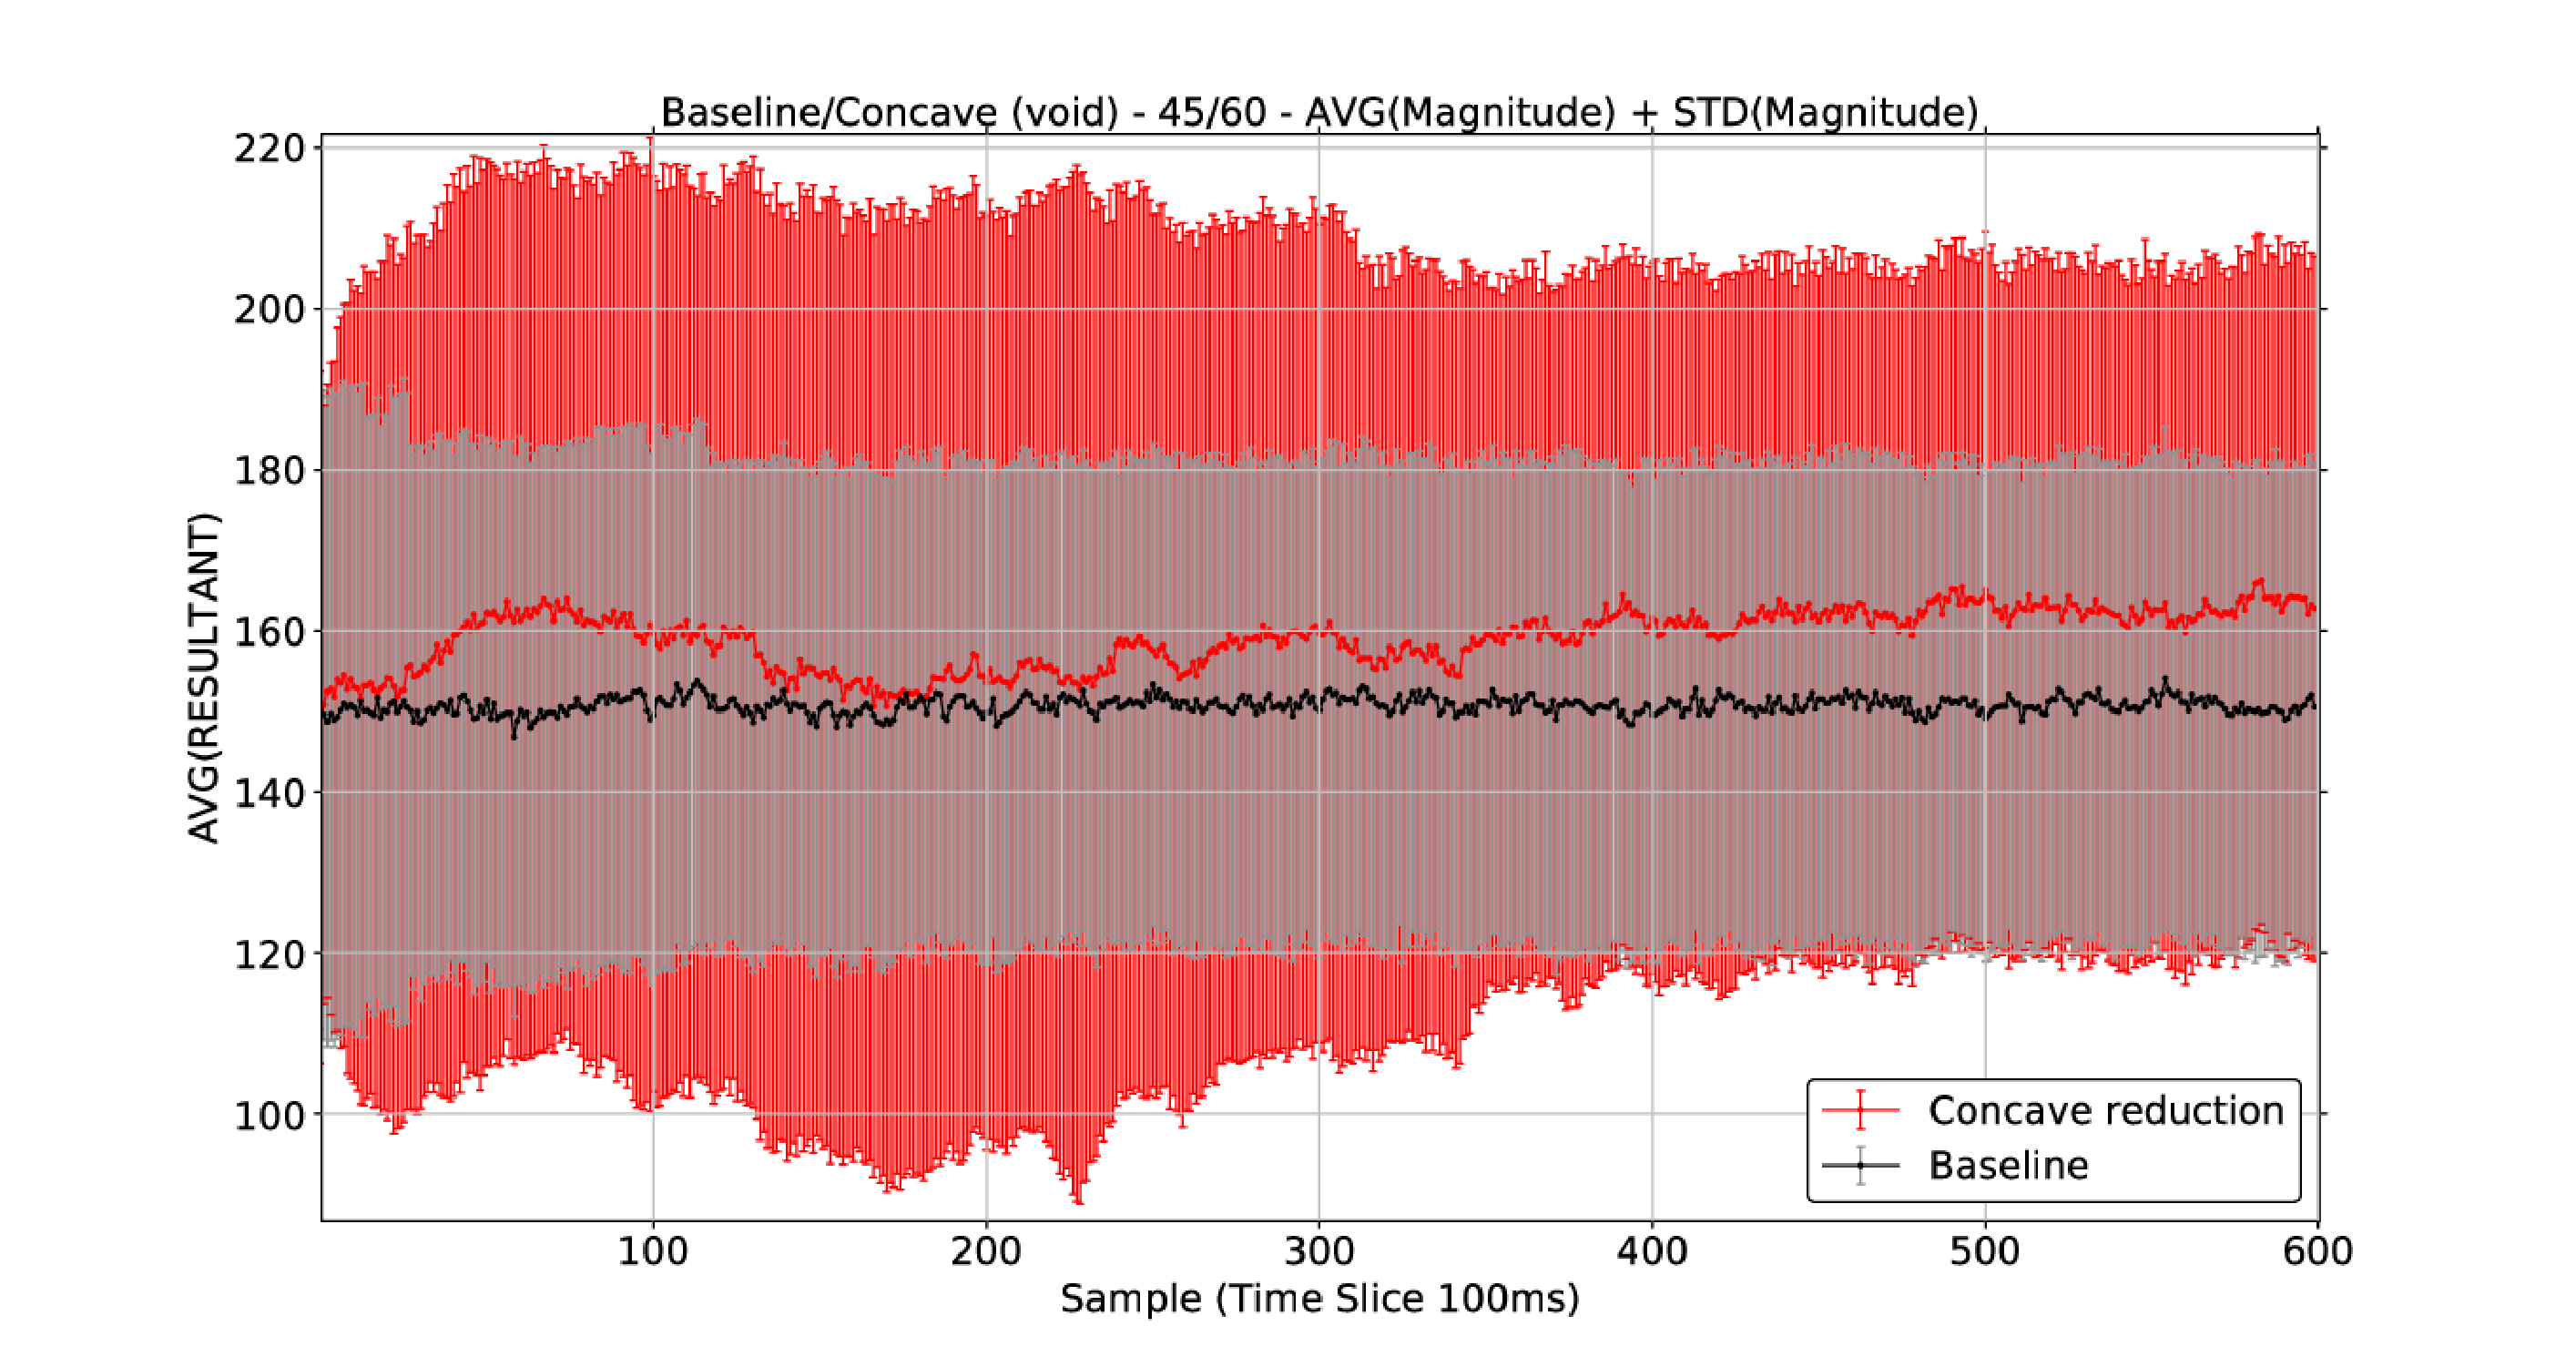
\includegraphics[width=8cm]{figures/ConcavePerimeter4560-MAG}
%% \end{center}
%% \caption{Concave reduction stability effect magnitude\label{voids:ConcavePerimeter4560-MAG}}
%% \end{figure}
Once the void is removed the swarm settles to a more stable phase 3.5 seconds on-wards~(Fig.~\ref{voids:ConcavePerimeter4560-MAG-2}), there is a slightly higher variance than the baseline which is caused by the concave reduction affected agents `pulling' the swarm. This `pulling' causes the agents to be slightly more distributed and therefore increases the inter-agent cohesion. There is also the addition of the `snapping' effect which increases the variance. 
%SWARMHOLE-MAG-4560.py
\Figure[t!](topskip=0pt, botskip=0pt, midskip=0pt)[width=8.3cm]{figures/ConcavePerimeter4560-MAG-2}{Concave reduction stability effect magnitude\label{voids:ConcavePerimeter4560-MAG-2}}
%% \begin{figure}
%% \begin{center}
%% 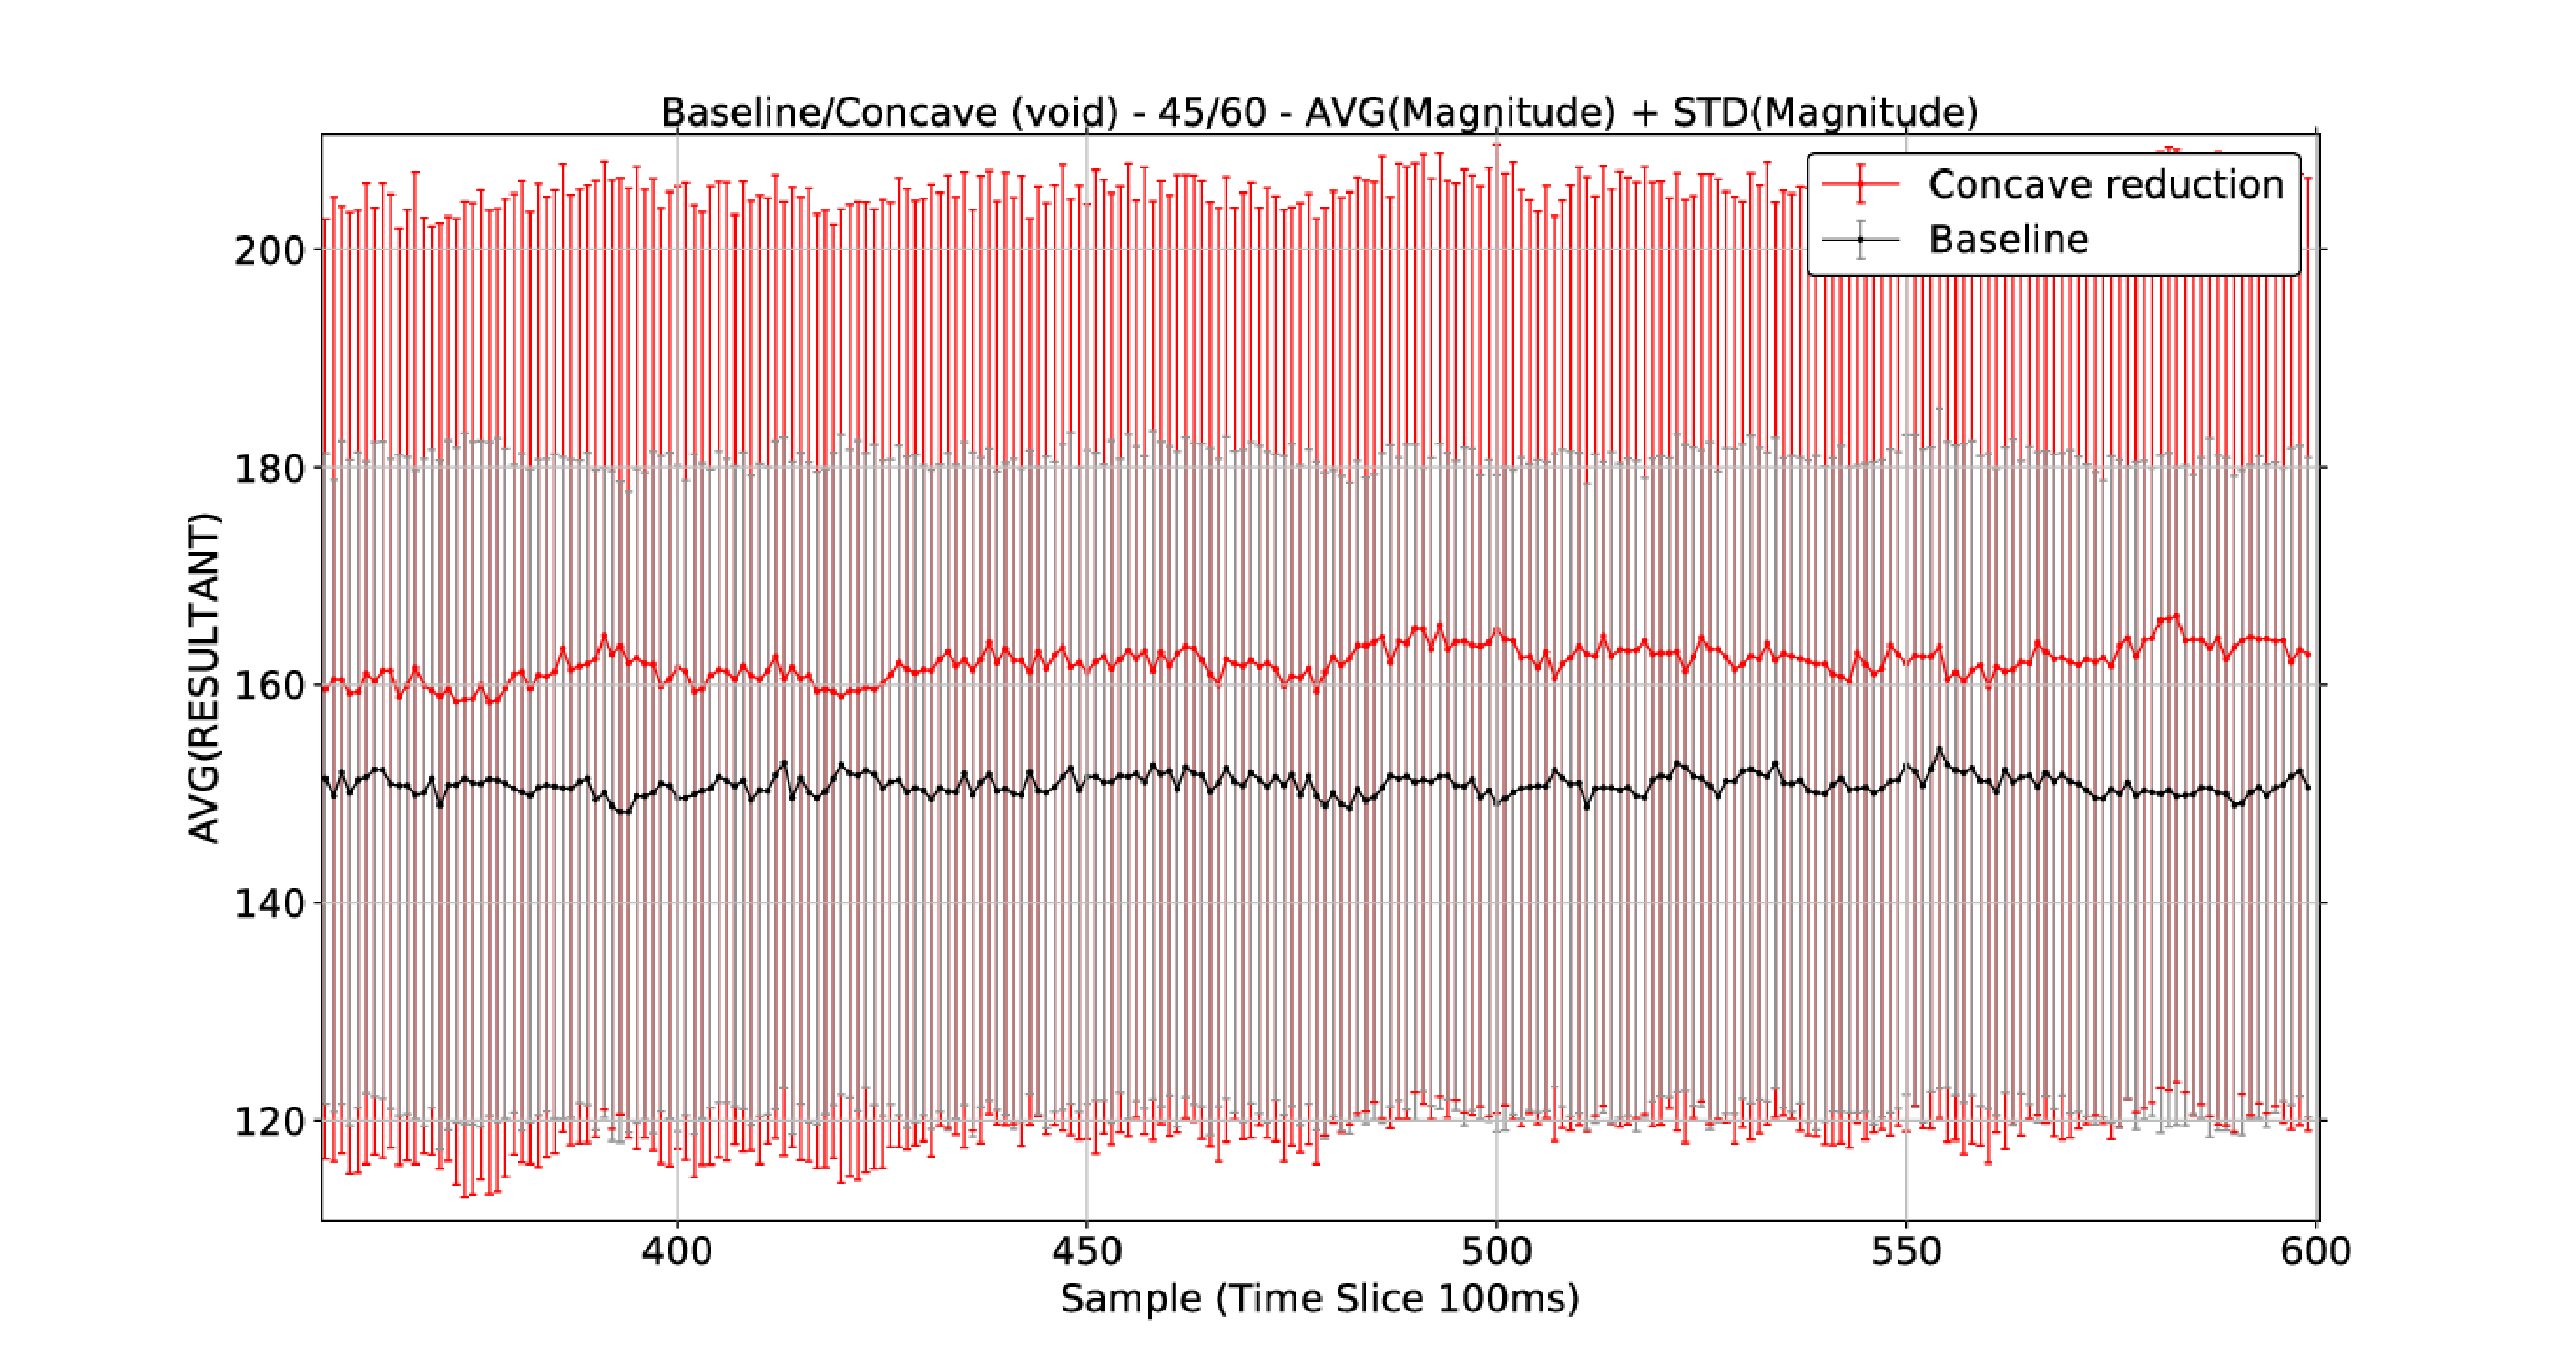
\includegraphics[width=8cm]{figures/ConcavePerimeter4560-MAG-2}
%% \end{center}
%% \caption{Concave reduction stability effect magnitude\label{voids:ConcavePerimeter4560-MAG-2}}
%% \end{figure}
The effect on the swarm of removing the void is to reduce the overall number of perimeter agents. Figure~\ref{methods:ConcavePerimeter4560-1} shows that as the void is removed from the swarm the number of perimeter agents falls. The change in size is caused by two processes. The swarm structure is being altered on the outer perimeter as the agents move towards a more circular formation and the internal agents identified as perimeter agents of a void move to reduce the internal anomaly. 
Once the initial distributions chaotic phase settles, which takes approximately 1.2 seconds, the effect of the concave reduction starts to take effect. The perimeter size starts to reduce. The majority of the reduction is the void shrinking. The swarm then goes through a settling period where the overall perimeter size of the swarm stabalises and eventually the residual snapping effect is left at the outer perimeter. This occurs at approximately 3.5 seconds into the simulation. 
%PERIMETER4560HOLE.py
\Figure[t!](topskip=0pt, botskip=0pt, midskip=0pt)[width=8.3cm]{figures/ConcavePerimeter4560-1}{Concave reduction perimeter effect\label{methods:ConcavePerimeter4560-1}}
%% \begin{figure}
%% \begin{center}
%% 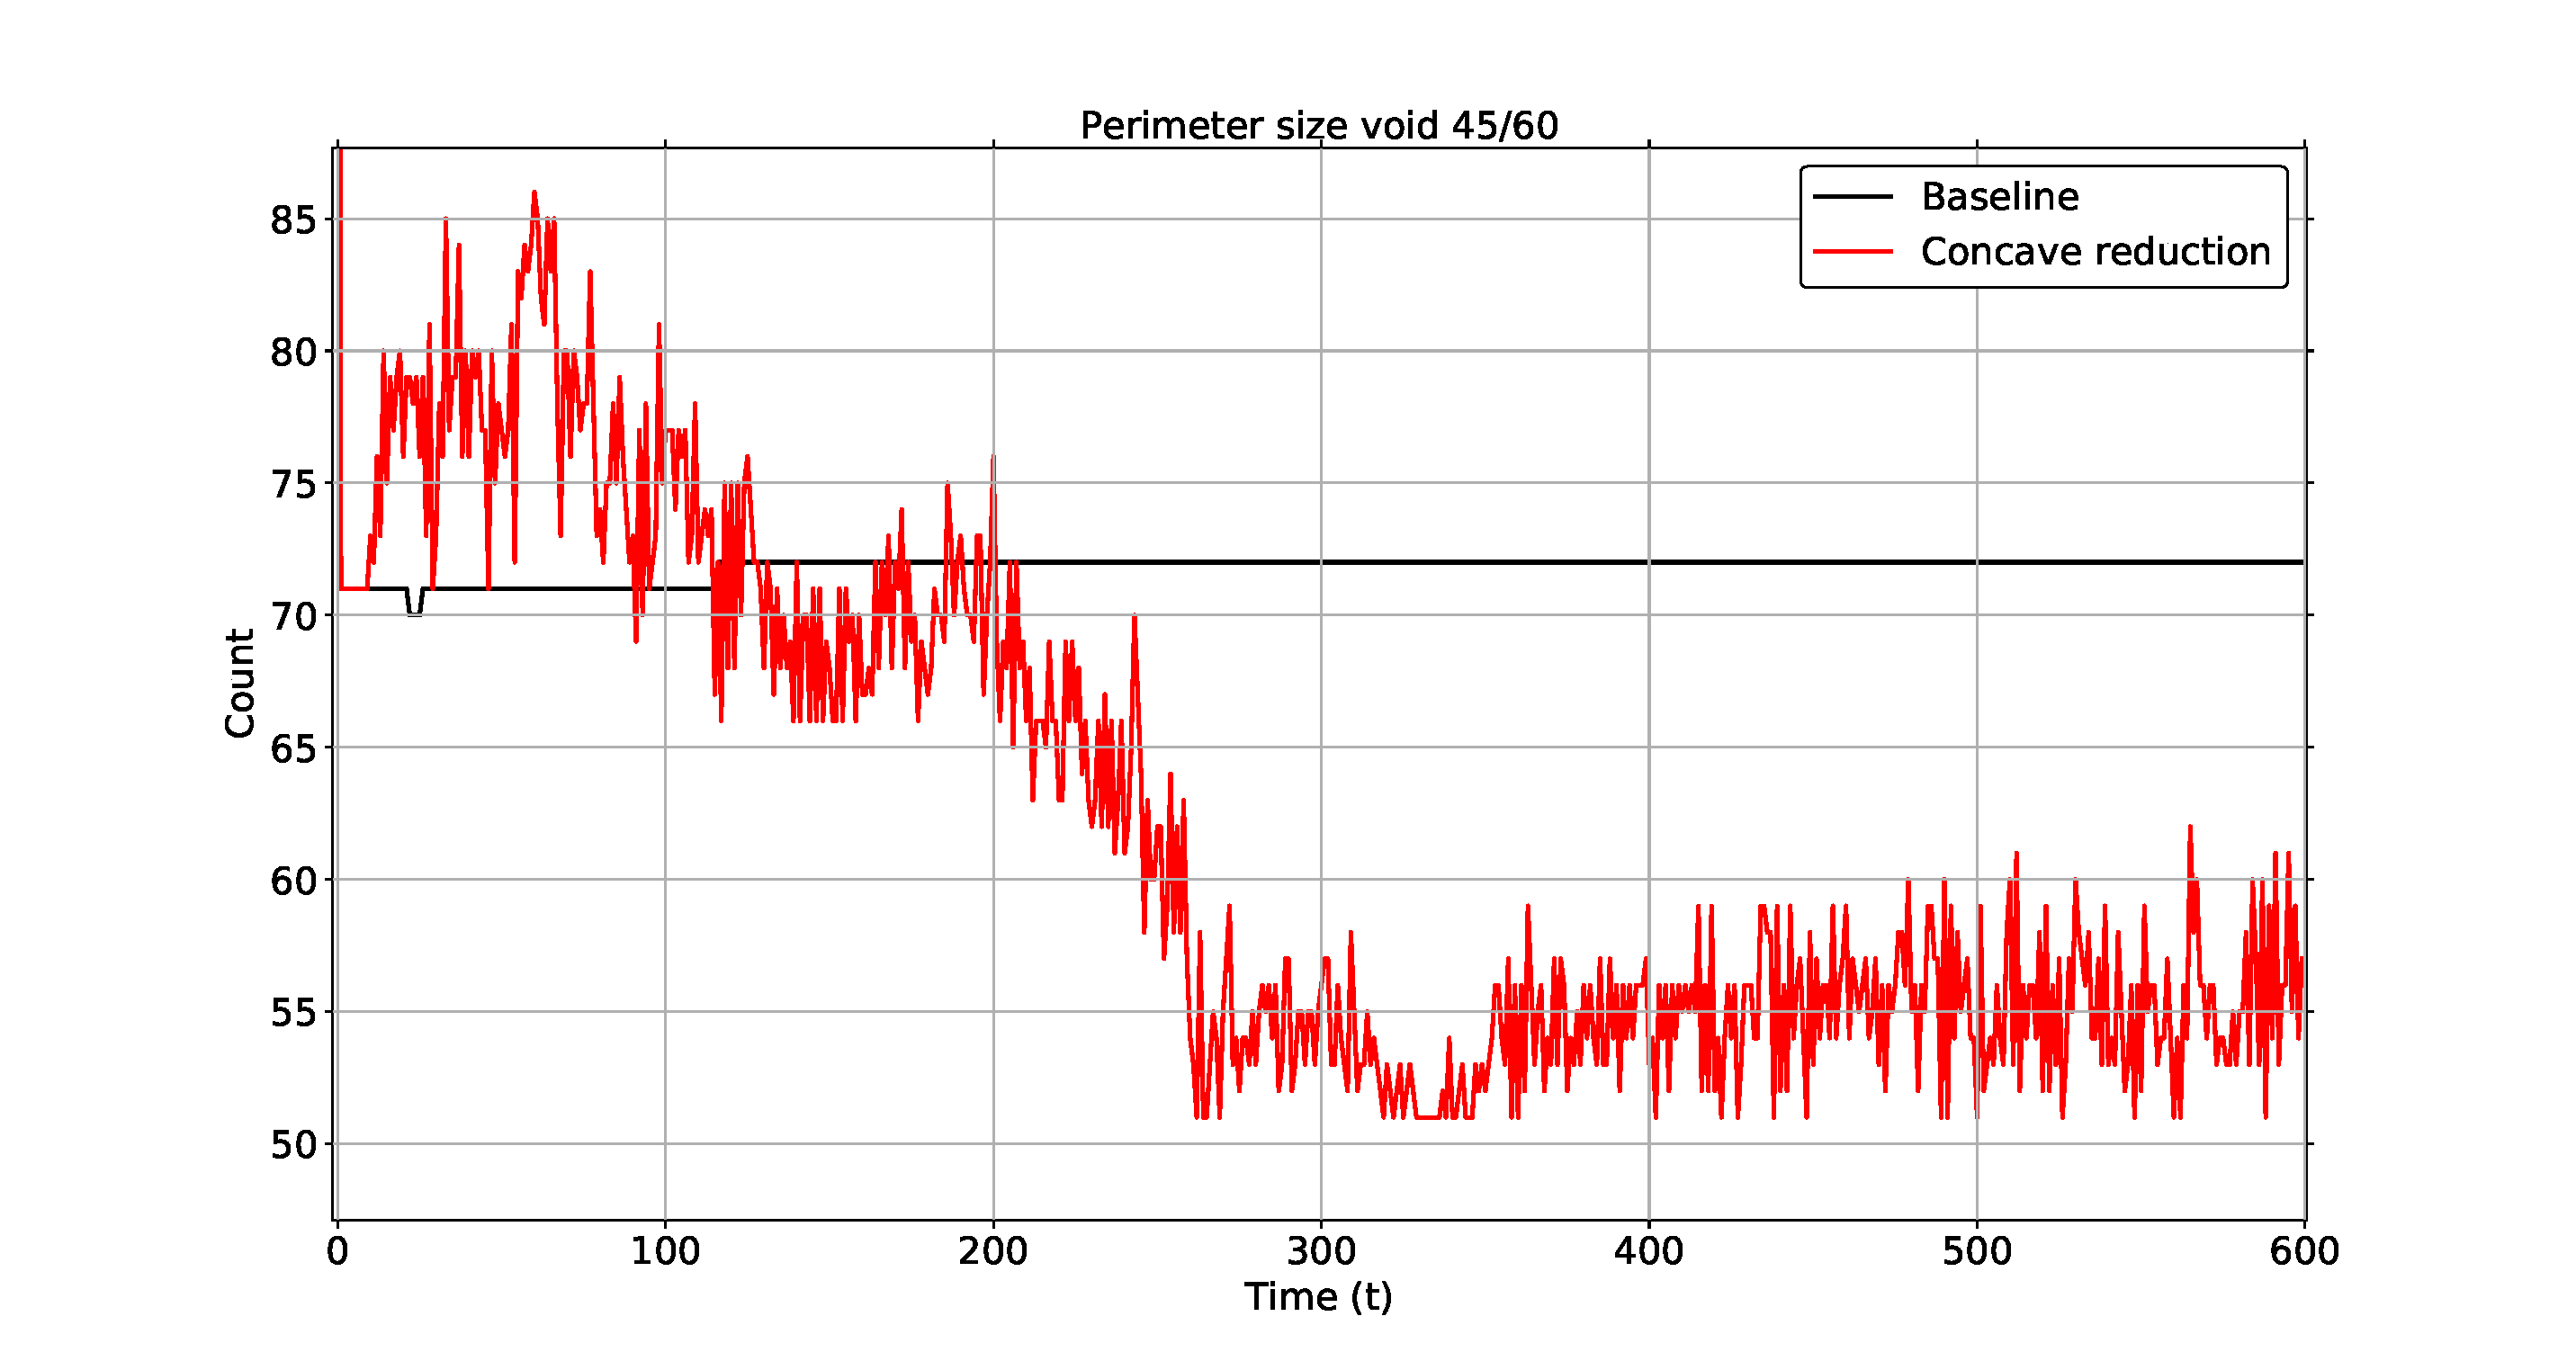
\includegraphics[width=8cm]{figures/ConcavePerimeter4560-1}
%% \end{center}
%% \caption{Concave reduction perimeter effect\label{methods:ConcavePerimeter4560-1}}
%% \end{figure}
The effect on the swarms structure is shown in Fig.~\ref{voids:SwarmCoverage4560-1} and~\ref{voids:SwarmCoverage4560-2}. Figure~\ref{voids:SwarmCoverage4560-1} shows the agents positions during the simulation for the baseline and the concave reduction enabled swarms. The baseline swarm is shown in black. The red traces are for the swarm using concave reduction. Figure~\ref{voids:SwarmCoverage4560-2} is a more detailed view highlighting the baseline lattice structure.
%COVERBASELINE4560.py
\Figure[t!](topskip=0pt, botskip=0pt, midskip=0pt)[width=8.3cm]{figures/SwarmCoverage4560-1}{Agent movement comparison\label{voids:SwarmCoverage4560-1}}
%% \begin{figure}
%% \begin{center}
%% 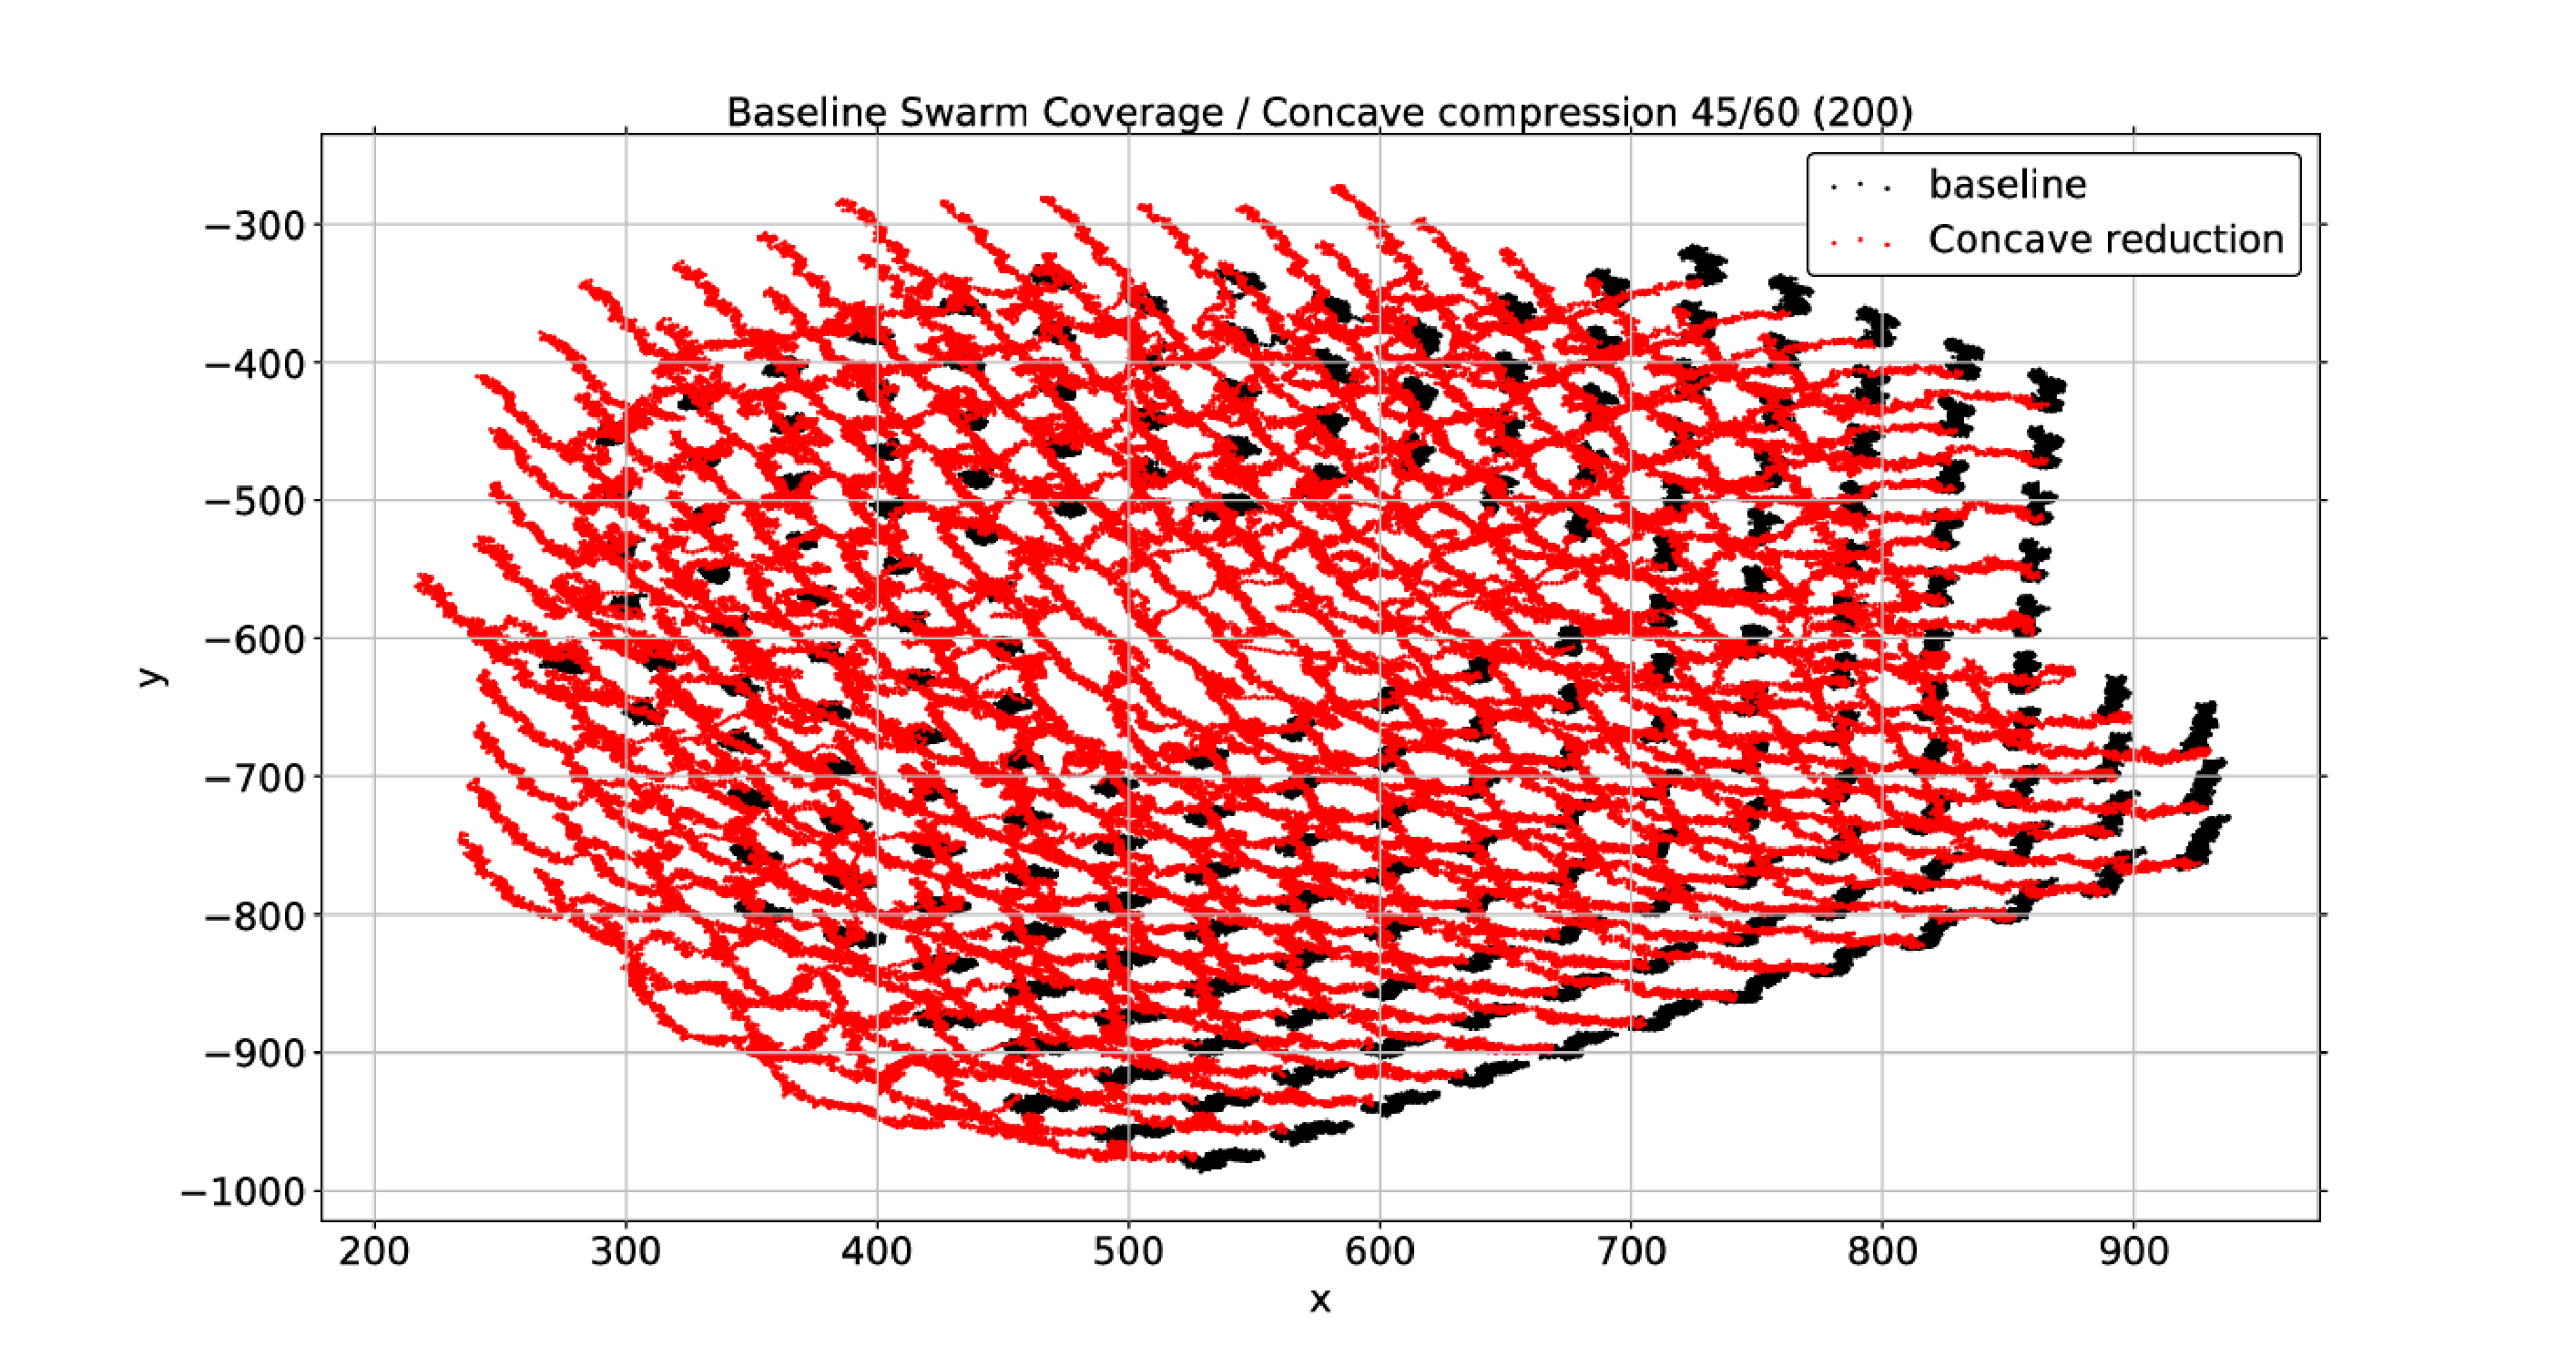
\includegraphics[width=8cm]{figures/SwarmCoverage4560-1}
%% \end{center}
%% \caption{Agent movement comparison\label{voids:SwarmCoverage4560-1}}
%% \end{figure}
The overall effect of the concave reduction on the swarms movement can be seen in~Fig.~\ref{voids:SwarmCoverage4560-1}. The void is closed by the reduction and the overall area of the swarm is reduced. There is however a negative effect with respect to the concave reduction; the swarm has a directional bias due to the large straight edge which causes the swarm to `drift'. When looking closely at the positions (Fig.~\ref{voids:SwarmCoverage4560-2}) the baseline agents remain relatively static in their positions vibrating slightly to maintain the equilibrium of the internal magnitudes. 
%COVERBASELINE4560.py
\Figure[t!](topskip=0pt, botskip=0pt, midskip=0pt)[width=8.3cm]{figures/SwarmCoverage4560-2}{Agent movement comparison\label{voids:SwarmCoverage4560-2}}
%% \begin{figure}
%% \begin{center}
%% 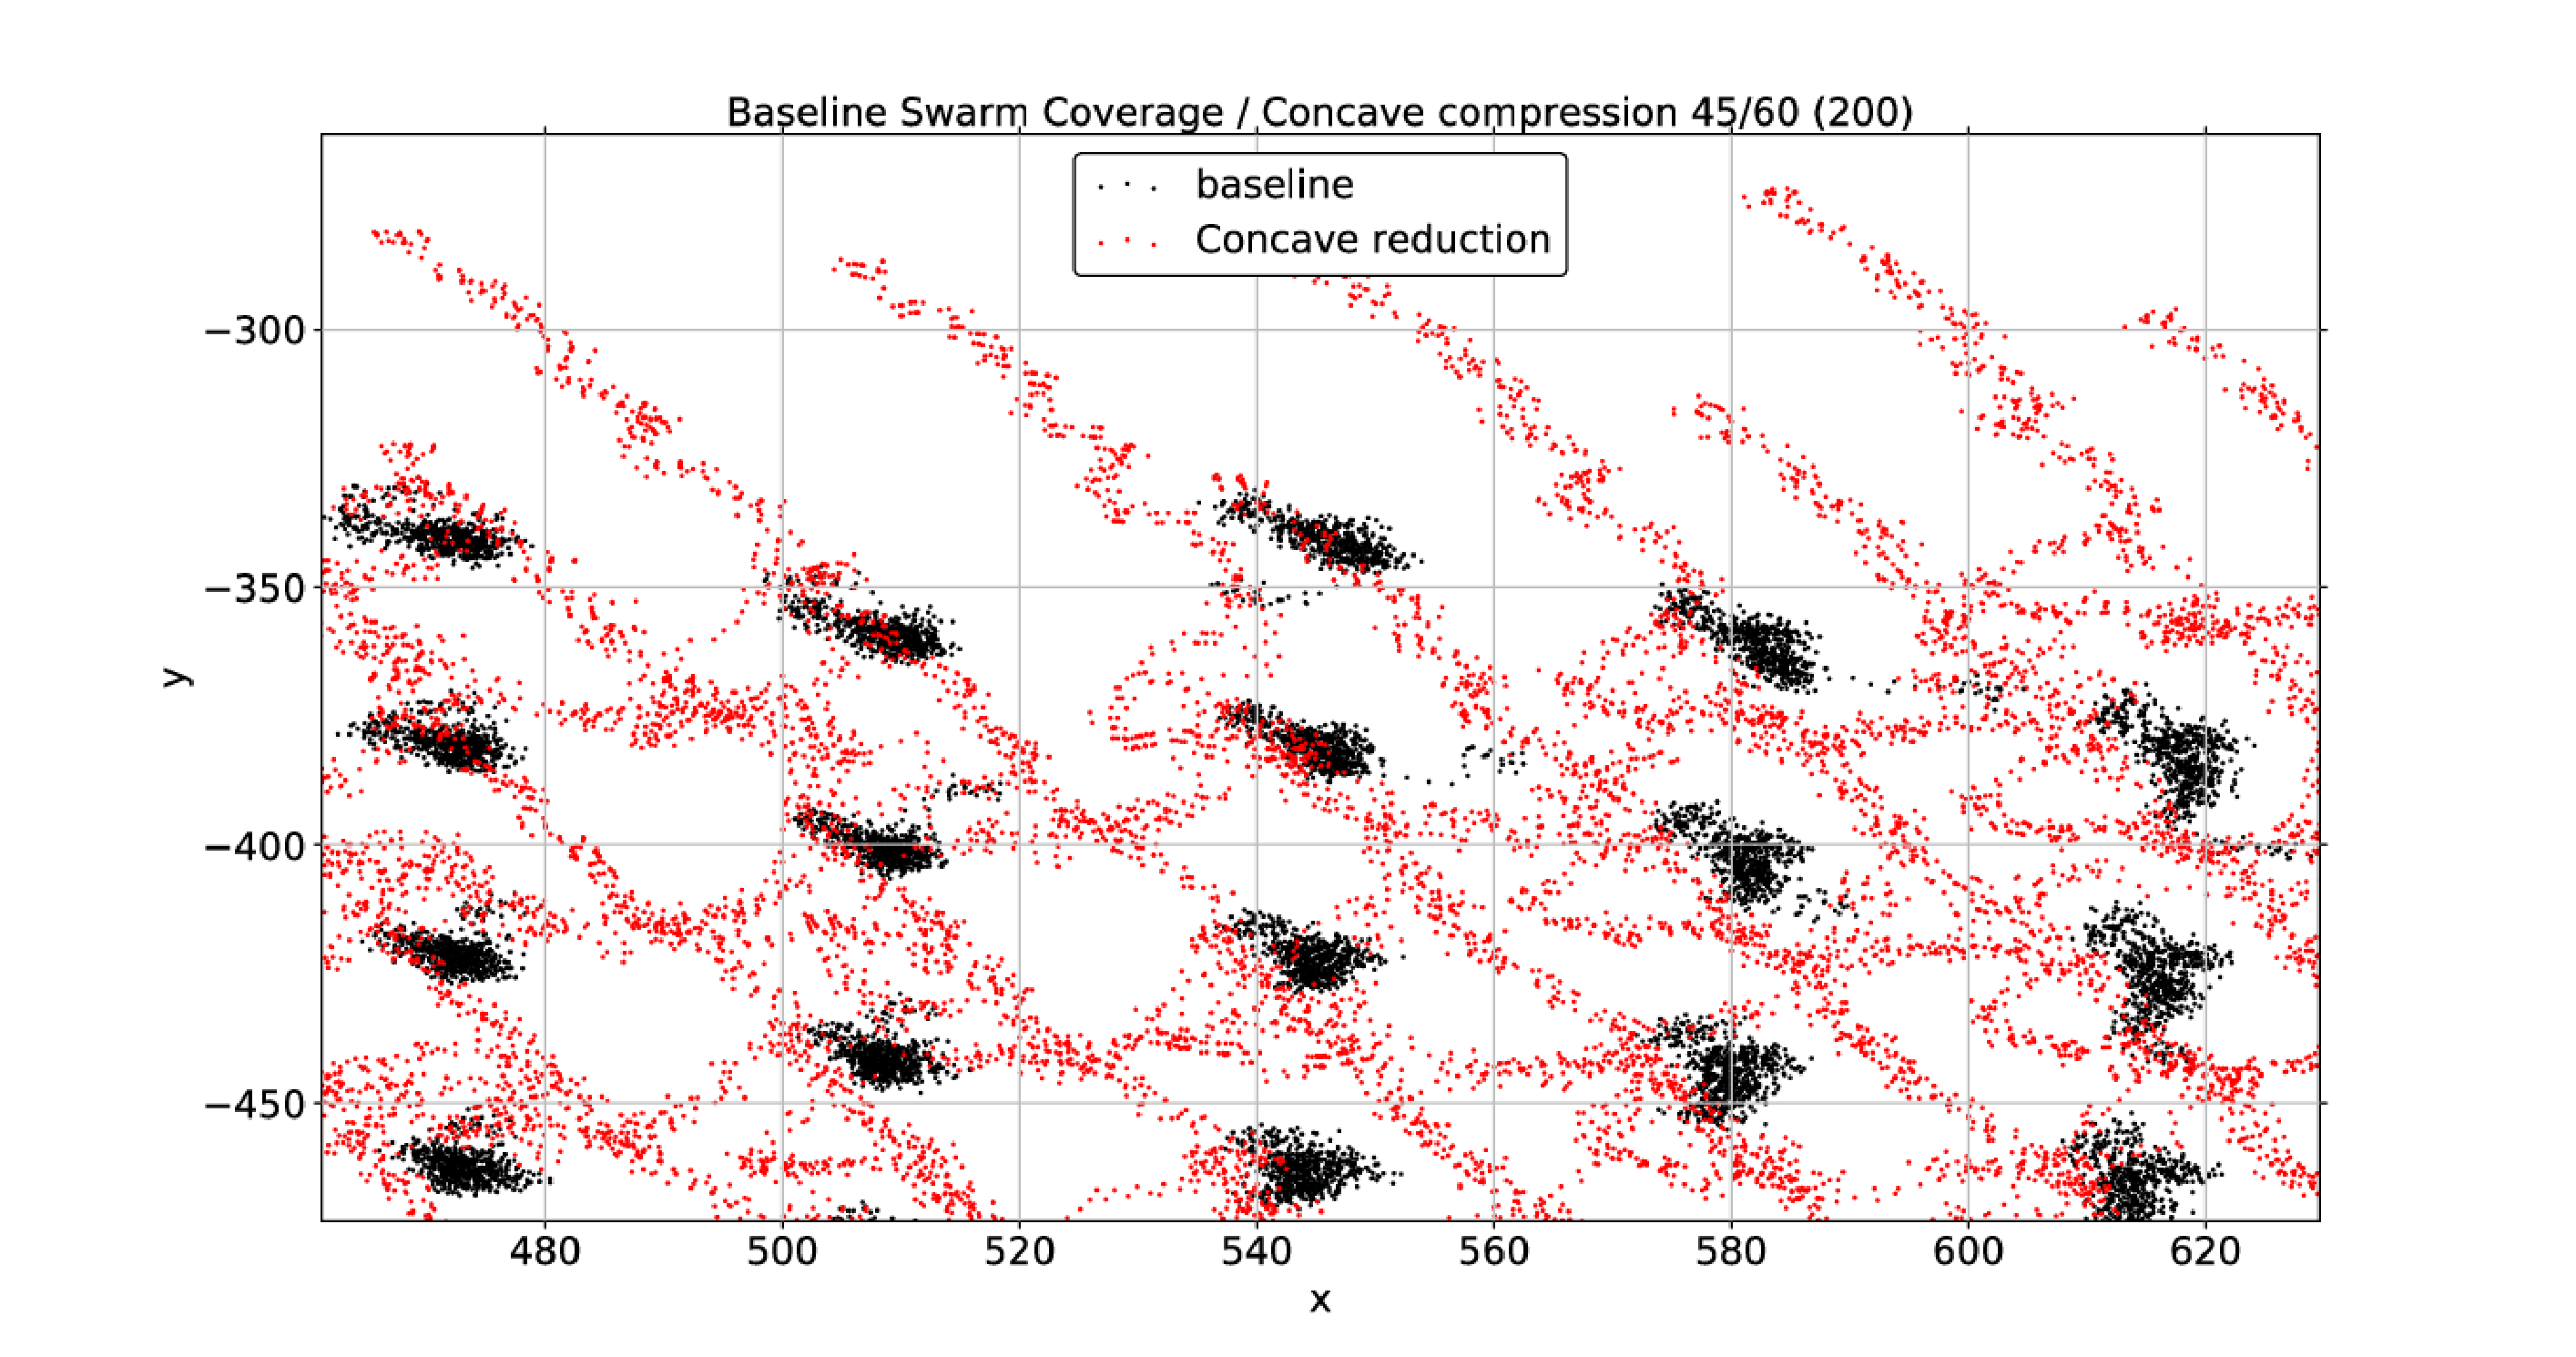
\includegraphics[width=8cm]{figures/SwarmCoverage4560-2}
%% \end{center}
%% \caption{Agent movement comparison\label{voids:SwarmCoverage4560-2}}
%% \end{figure}
\section{Concave reduction for object surrounding}\label{voids:ObjectSurrounding}
Concave reduction has the benefit of creating a convex-perimeter and removing a concave perimeter. This effect can be applied to surrounding objects. As a void is removed agents still avoid obstacles, this results in a perimeter edge that tightly encloses an object's perimeter. The concept of detecting an object and surrounding it is not new. In 2013 Zhang et al~\cite{ZFG:13} investigated this as a mechanism to assist in oil spillage containment. The process they used was based on ant-colony foraging. The agents initially carried out reconnaissance to detect a spillage, once a target is identified the agents use a communications infrastructure to inform nearby agents of the location of the spillage and the agents then use a \textit{destination vector} to locate the spill. To surround the spill the agents move in an anti-clockwise manner following the perimeter wall of the target. This paper uses a different approach to solve this same problem.
One problem with the above approach is that the swarm may not find the spillage due to the paths the agents take when foraging not intersecting with the spillage. Another problem is that the system does not consider multiple targets. Finally there is the issue of the swarm requiring a communications infrastructure. 
This paper focuses on arbitrary sized, low cost, swarms; this is a similar approach to the US Navy in the LOCUST project~\cite{MW:15, DS:15}. Also the approach of using concave reduction removes the need for a communications infrastructure. 
Consider an oil slick in an environment. This could be a section of open-water or a lake/reservoir. The solution is to deploy a swarm at the perimeter of the known area by a boat or at a shoreline if the area is small enough~(Fig.~\ref{voids:OilSlick}). The deployed agents, using local sensing and the concave reduction algorithm, are enabled. The swarm initially expands to an optimum distribution for the specified field effects. The \textit{concave reduction vector} will then reduce the deliberately created void and the swarm encapsulates the oil spill. If there are multiple spills within the area the void reduction process will still encapsulate the area because the algorithm is not dependant on communications and operates purely by logic.  

\Figure[t!](topskip=0pt, botskip=0pt, midskip=0pt)[width=8.3cm]{figures/OilSlick}{Concave reduction oil slick surrounding\label{voids:OilSlick}}
%% \begin{figure}
%% \begin{center}
%% 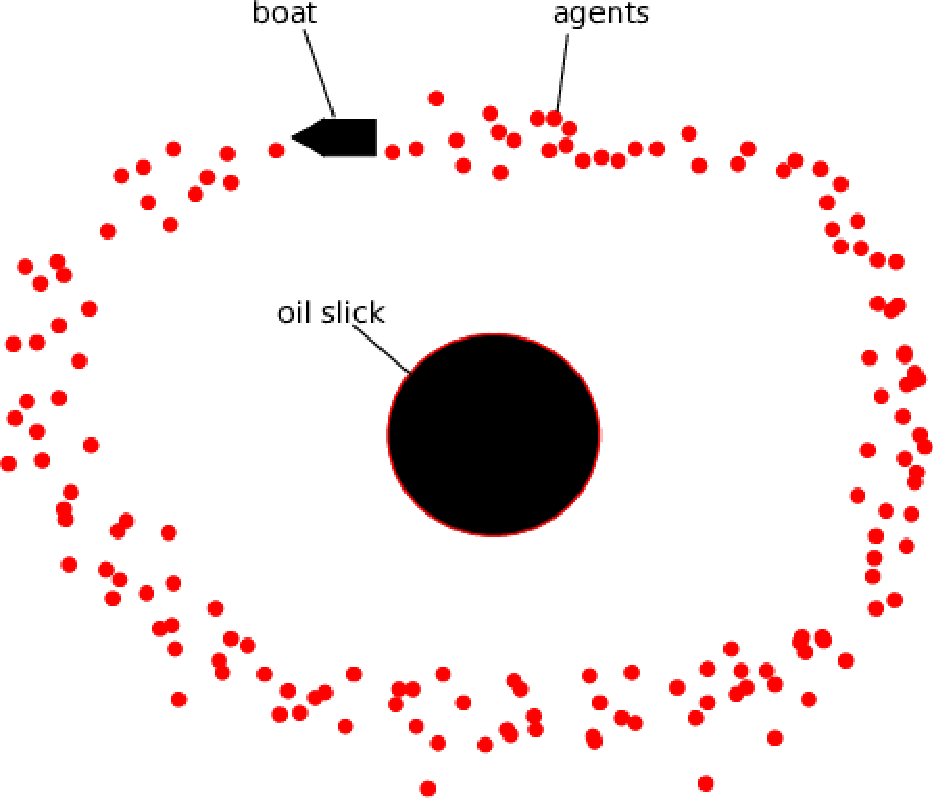
\includegraphics[width=8cm]{figures/OilSlick}
%% \end{center}
%% \caption{Concave reduction oil slick surrounding\label{voids:OilSlick}}
%% \end{figure}

Figure~\ref{concave:OilSpillSimulation} is a screen shot of the deployment within the simulator for testing this hypothesis. 

%==================== GRAPHS DONE TO HERE ===============================

\Figure[t!](topskip=0pt, botskip=0pt, midskip=0pt)[width=8.3cm]{figures/OilSpillSimulator}
{Oil spill containment simulation\label{concave:OilSpillSimulation}}
%% \begin{figure}
%% \begin{center}
%% 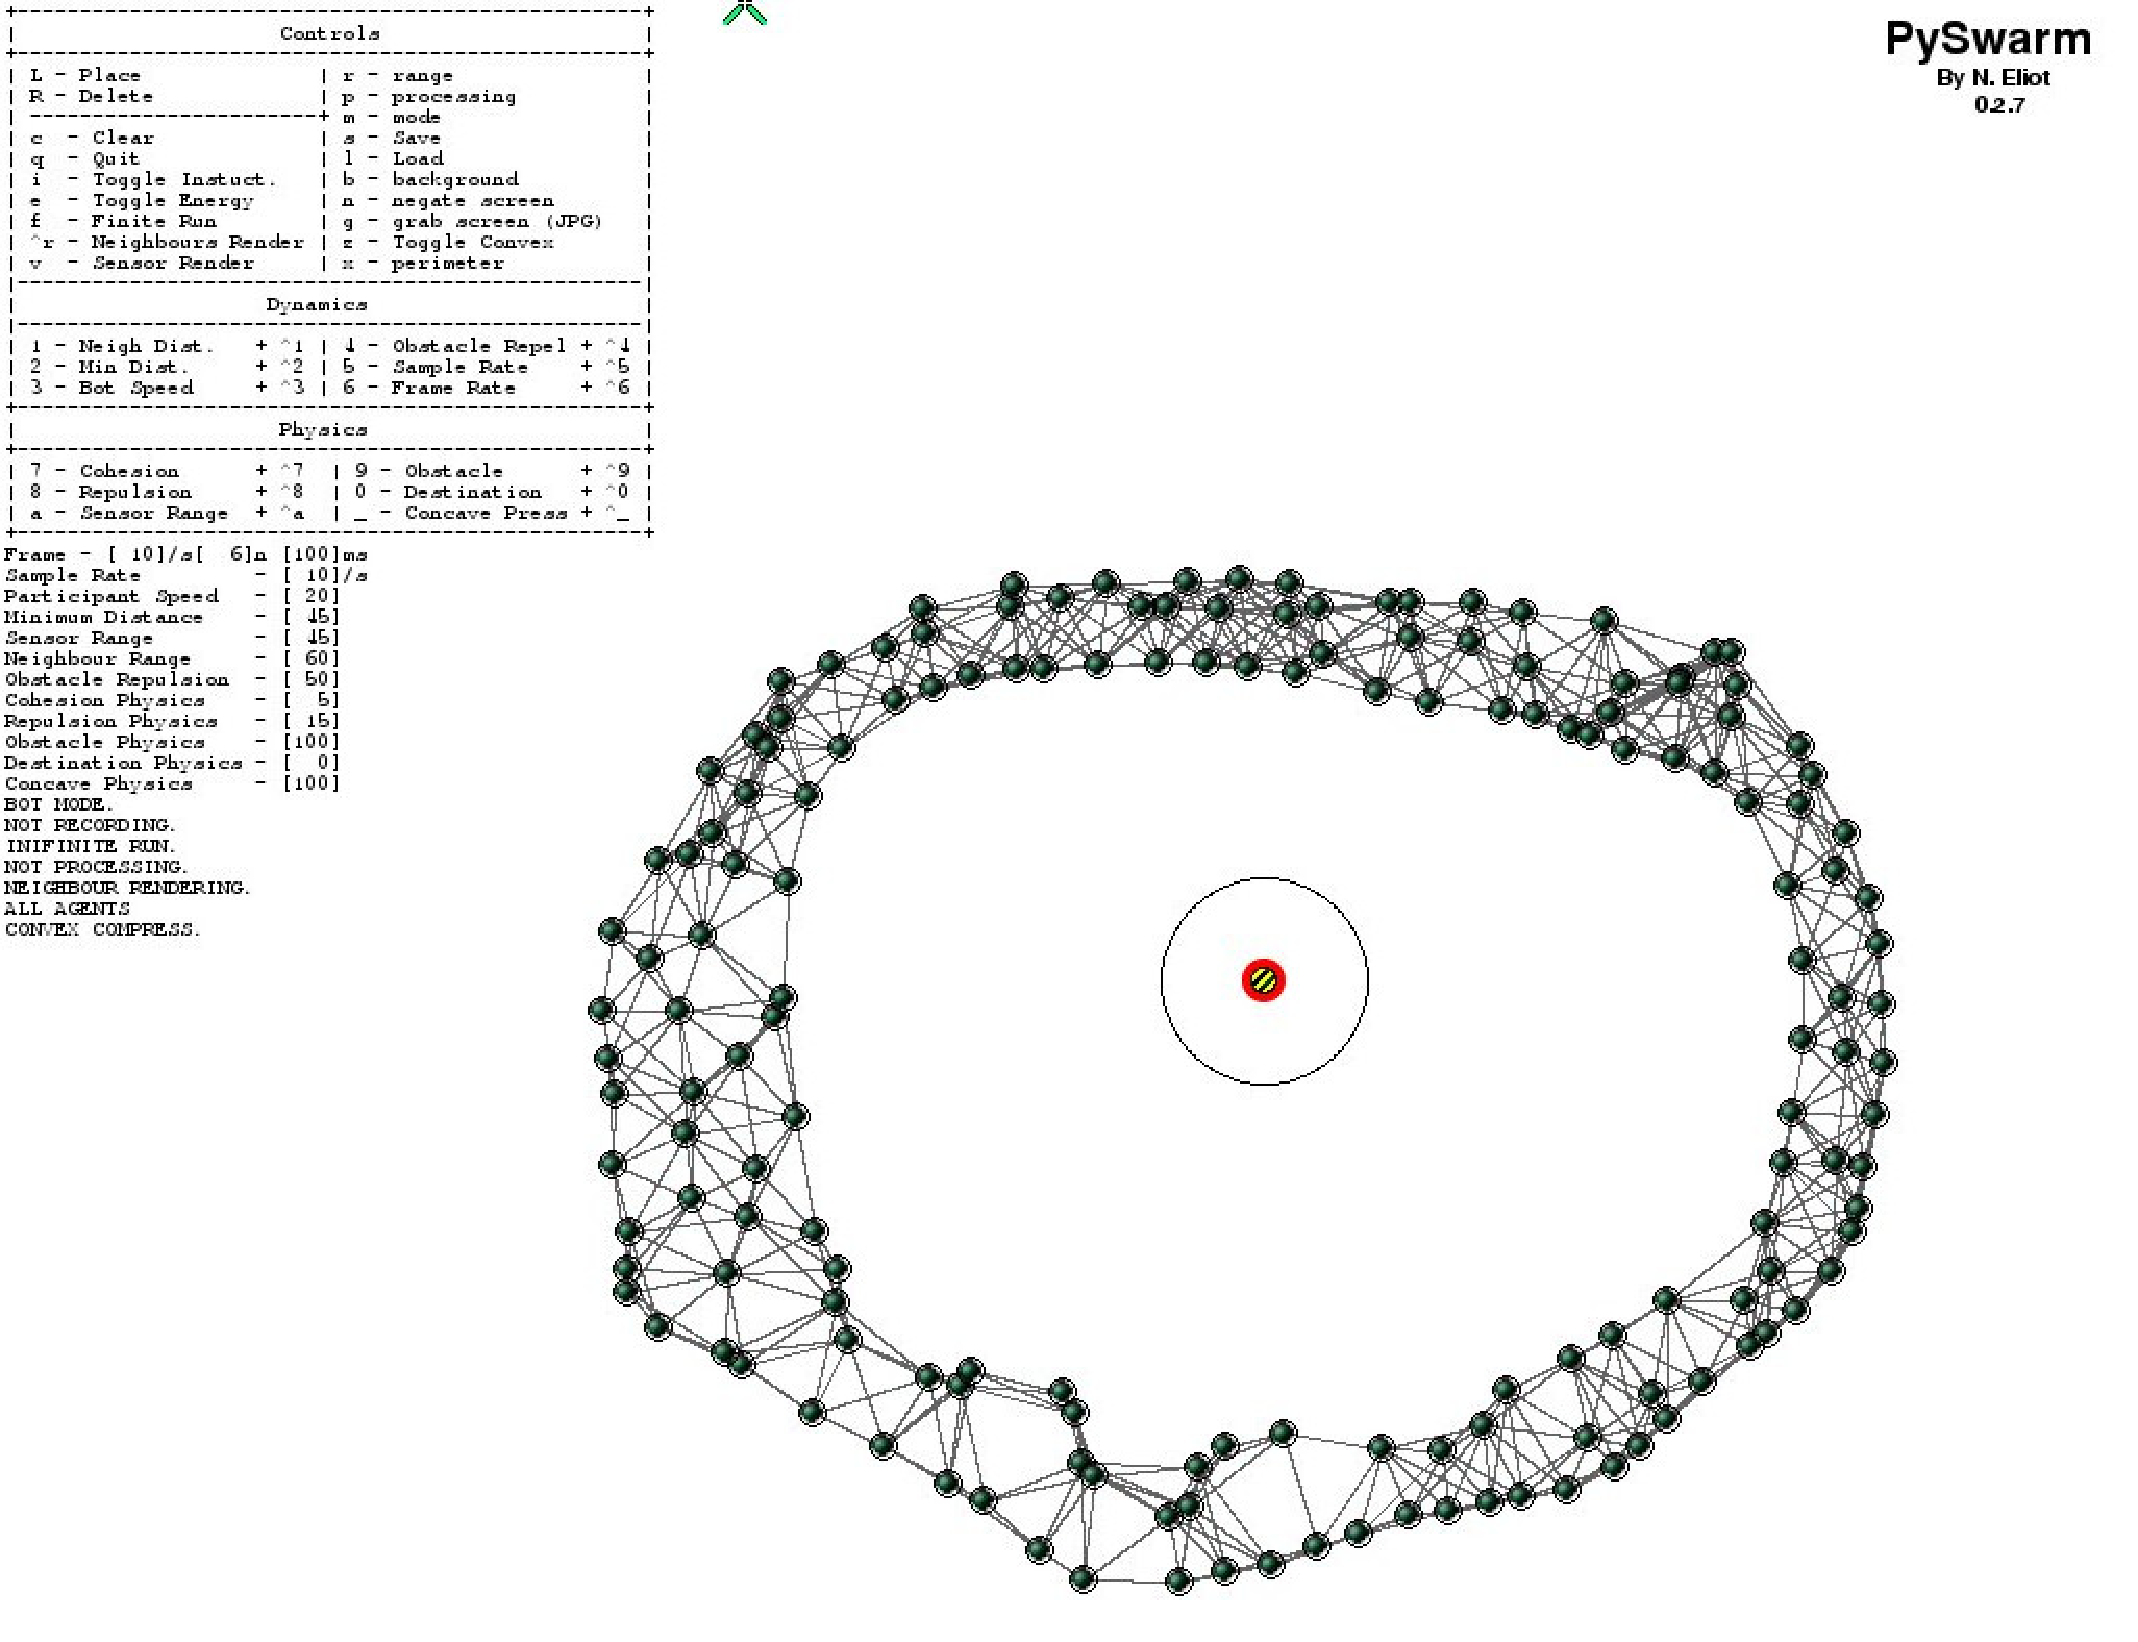
\includegraphics[width=8cm]{figures/OilSpillSimulator}
%% \end{center}
%% \caption{Oil spill containment simulation\label{concave:OilSpillSimulation}}
%% \end{figure}

Figure~\ref{concave:OilSpillBase1}, \ref{concave:OilSpillBase2} and \ref{concave:OilSpillBase3} shows the containment process using the baseline configuration without concave reduction. The swarm expands due to the field effects and then stabilises into a swarm which contains a void area. The swarm stablises and the swarm moves slightly as the cohesion and repulsion fluctuate to maintain the swarm's structure. However the void does not close and the containment process does not occur. The agents that do come in contact with the obstacle are repelled by the obstacle repulsion field.

%COVERBASELINE8060OILSPILL1.py
\Figure[t!](topskip=0pt, botskip=0pt, midskip=0pt)[width=8.3cm]{figures/OilSpillBase1}{Initial\label{concave:OilSpillBase1}}
%% \begin{figure}
%% \begin{center}
%% 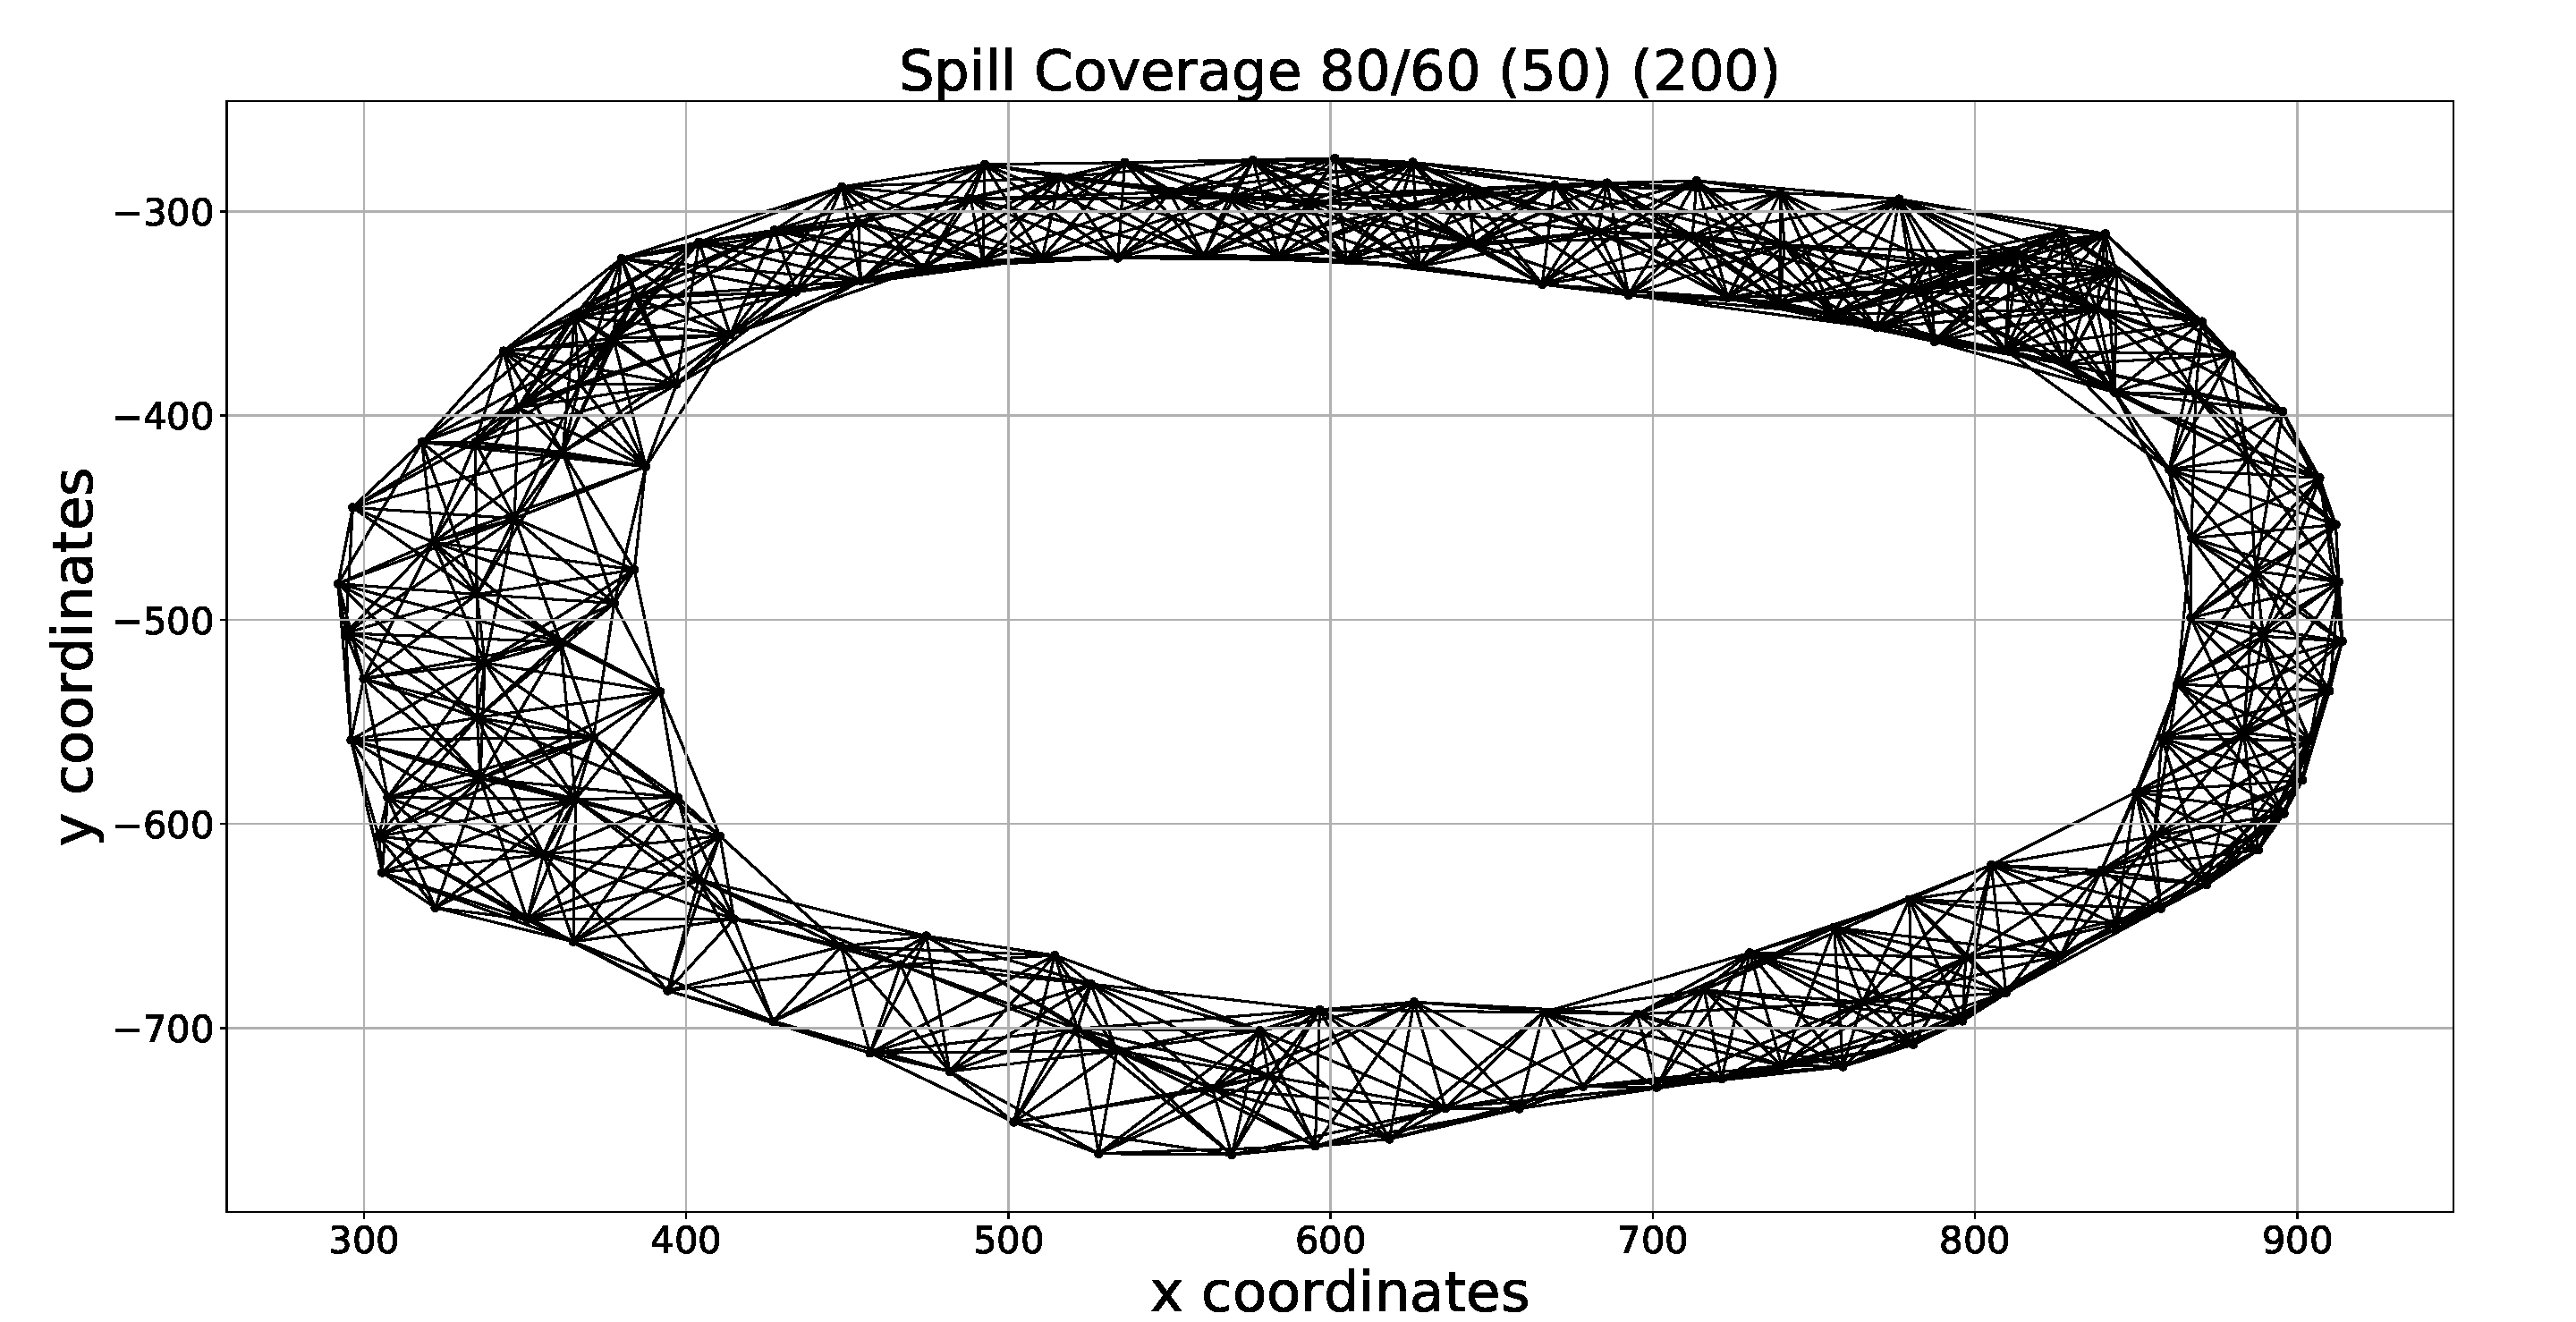
\includegraphics[with=5cm]{figures/OilSpillBase1}
%% \end{center}
%% \caption{Initial\label{concave:OilSpillBase1}}
%% \end{figure}
%COVERBASELINE8060OILSPILL3.py
\Figure[t!](topskip=0pt, botskip=0pt, midskip=0pt)[width=8.3cm]{figures/OilSpillBase2}{Partial\label{concave:OilSpillBase2}}
%% \begin{figure}
%% \begin{center}
%% 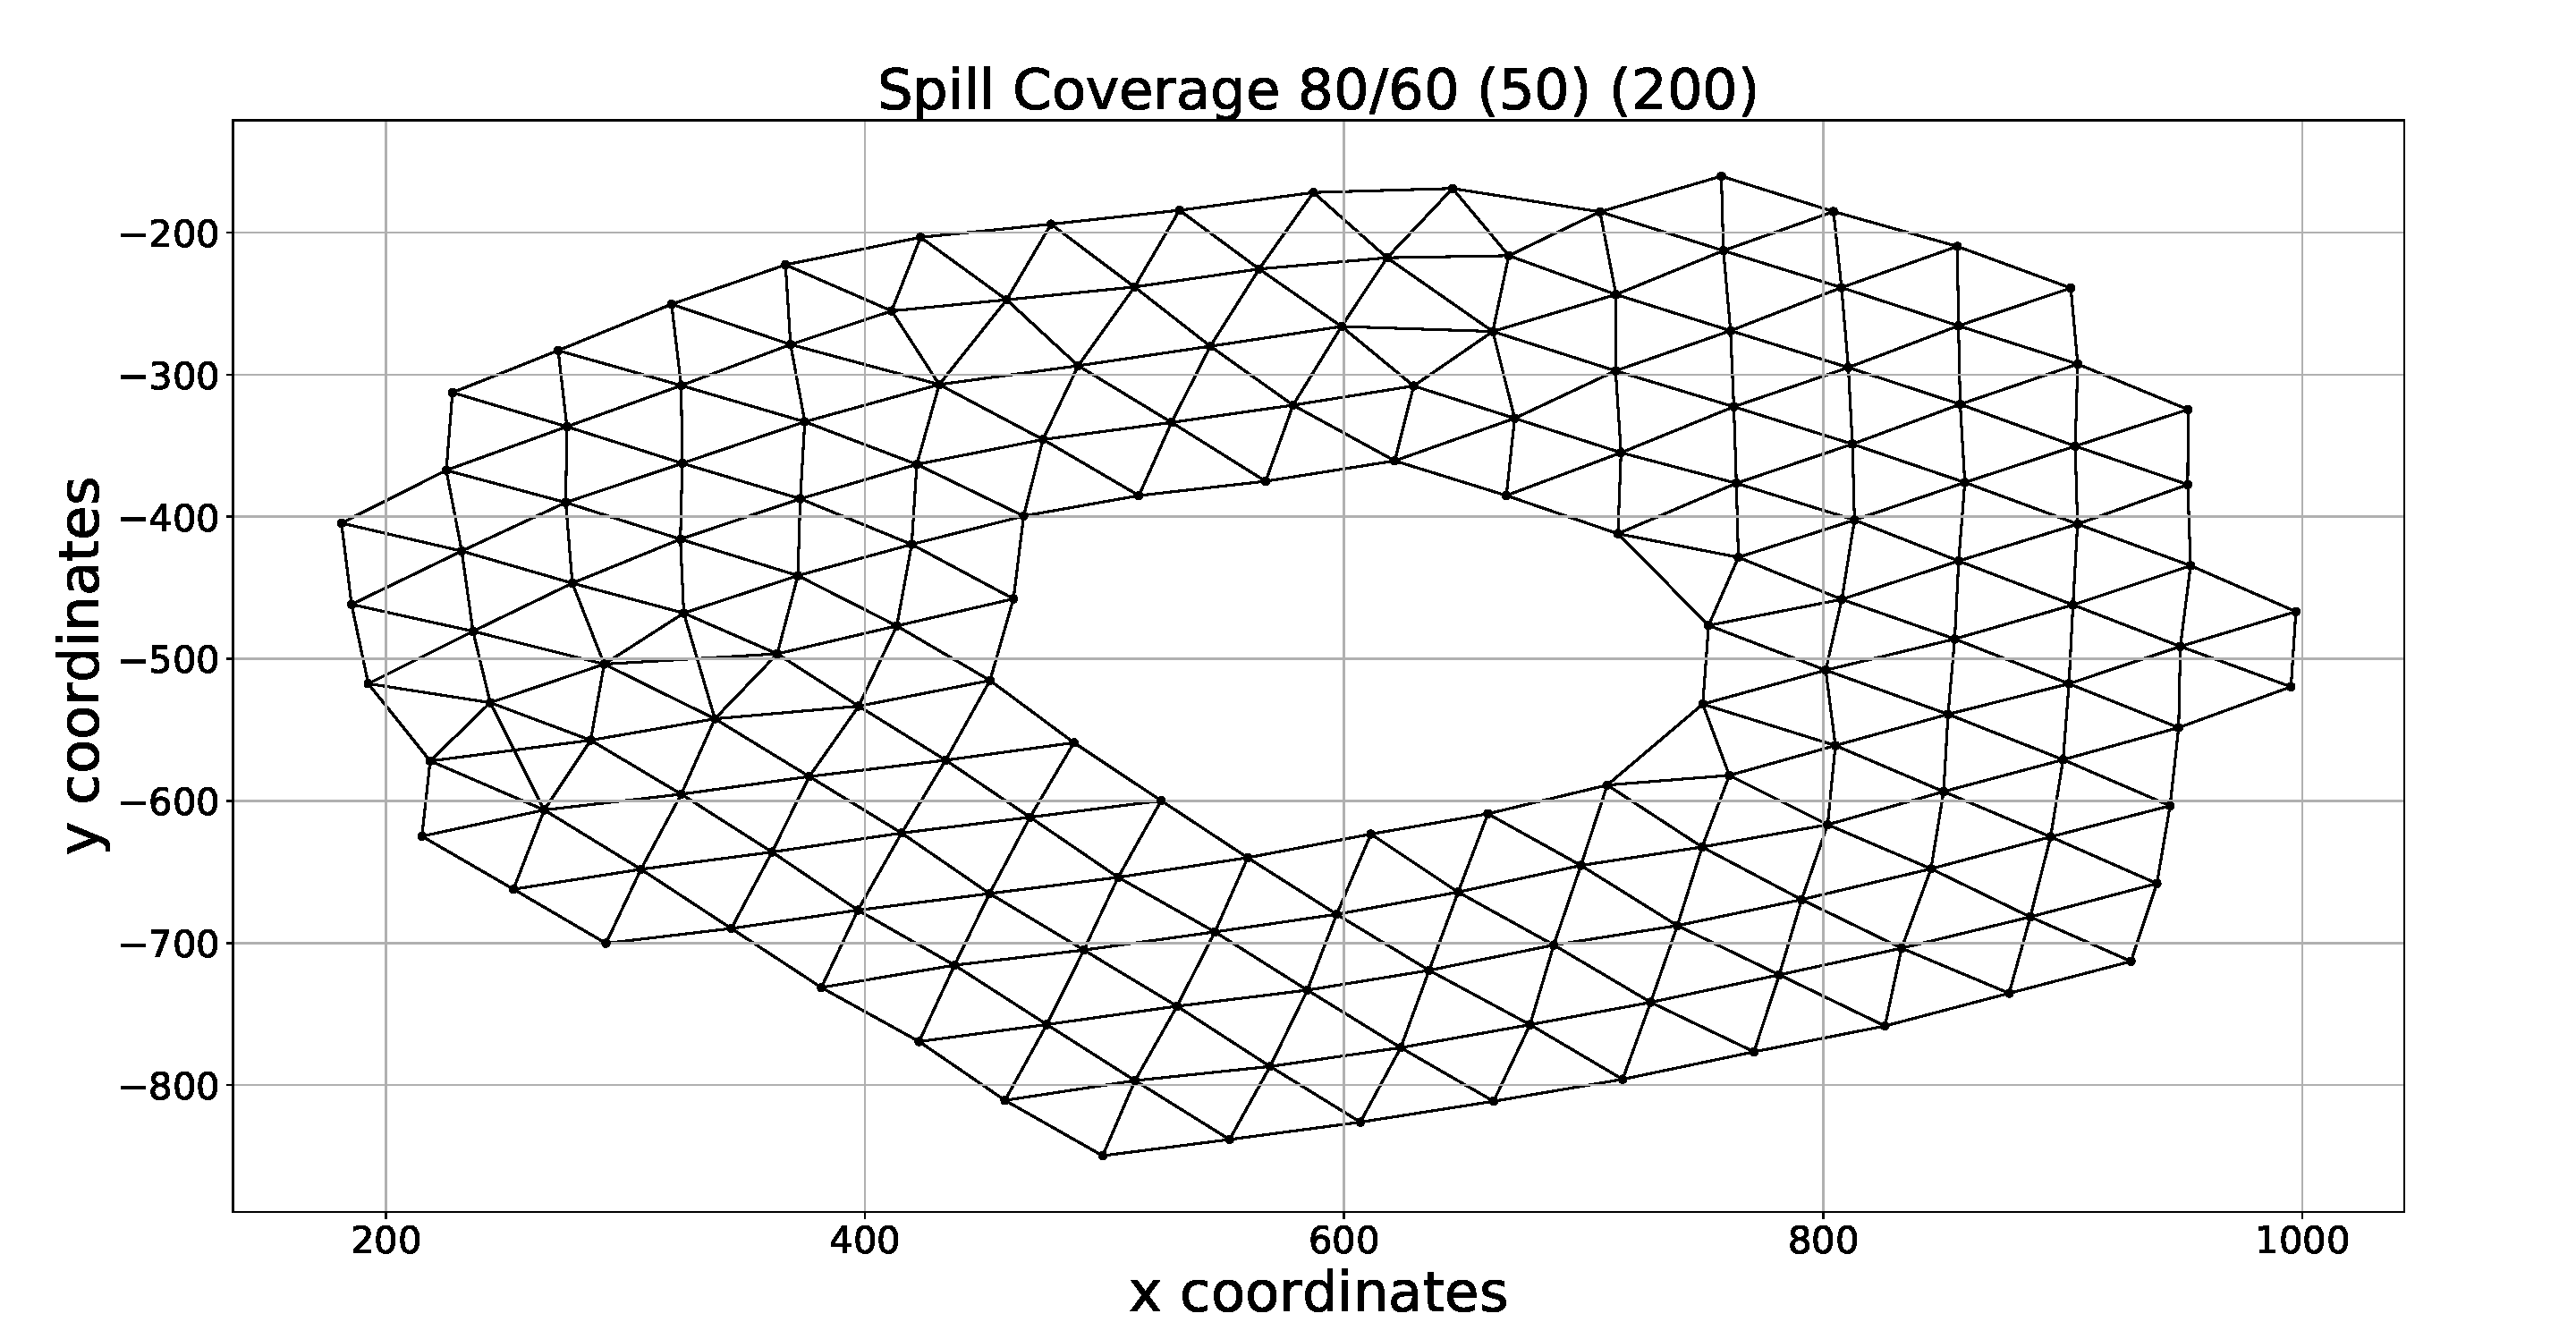
\includegraphics[width=5cm]{figures/OilSpillBase2}
%% \end{center}
%% \caption{Partial\label{concave:OilSpillBase2}}
%% \end{figure}
%COVERBASELINE8060OILSPILL3.py
\Figure[t!](topskip=0pt, botskip=0pt, midskip=0pt)[width=8.3cm]{figures/OilSpillBase3}{End\label{concave:OilSpillBase3}}
%% \begin{figure}
%% \begin{center}
%% 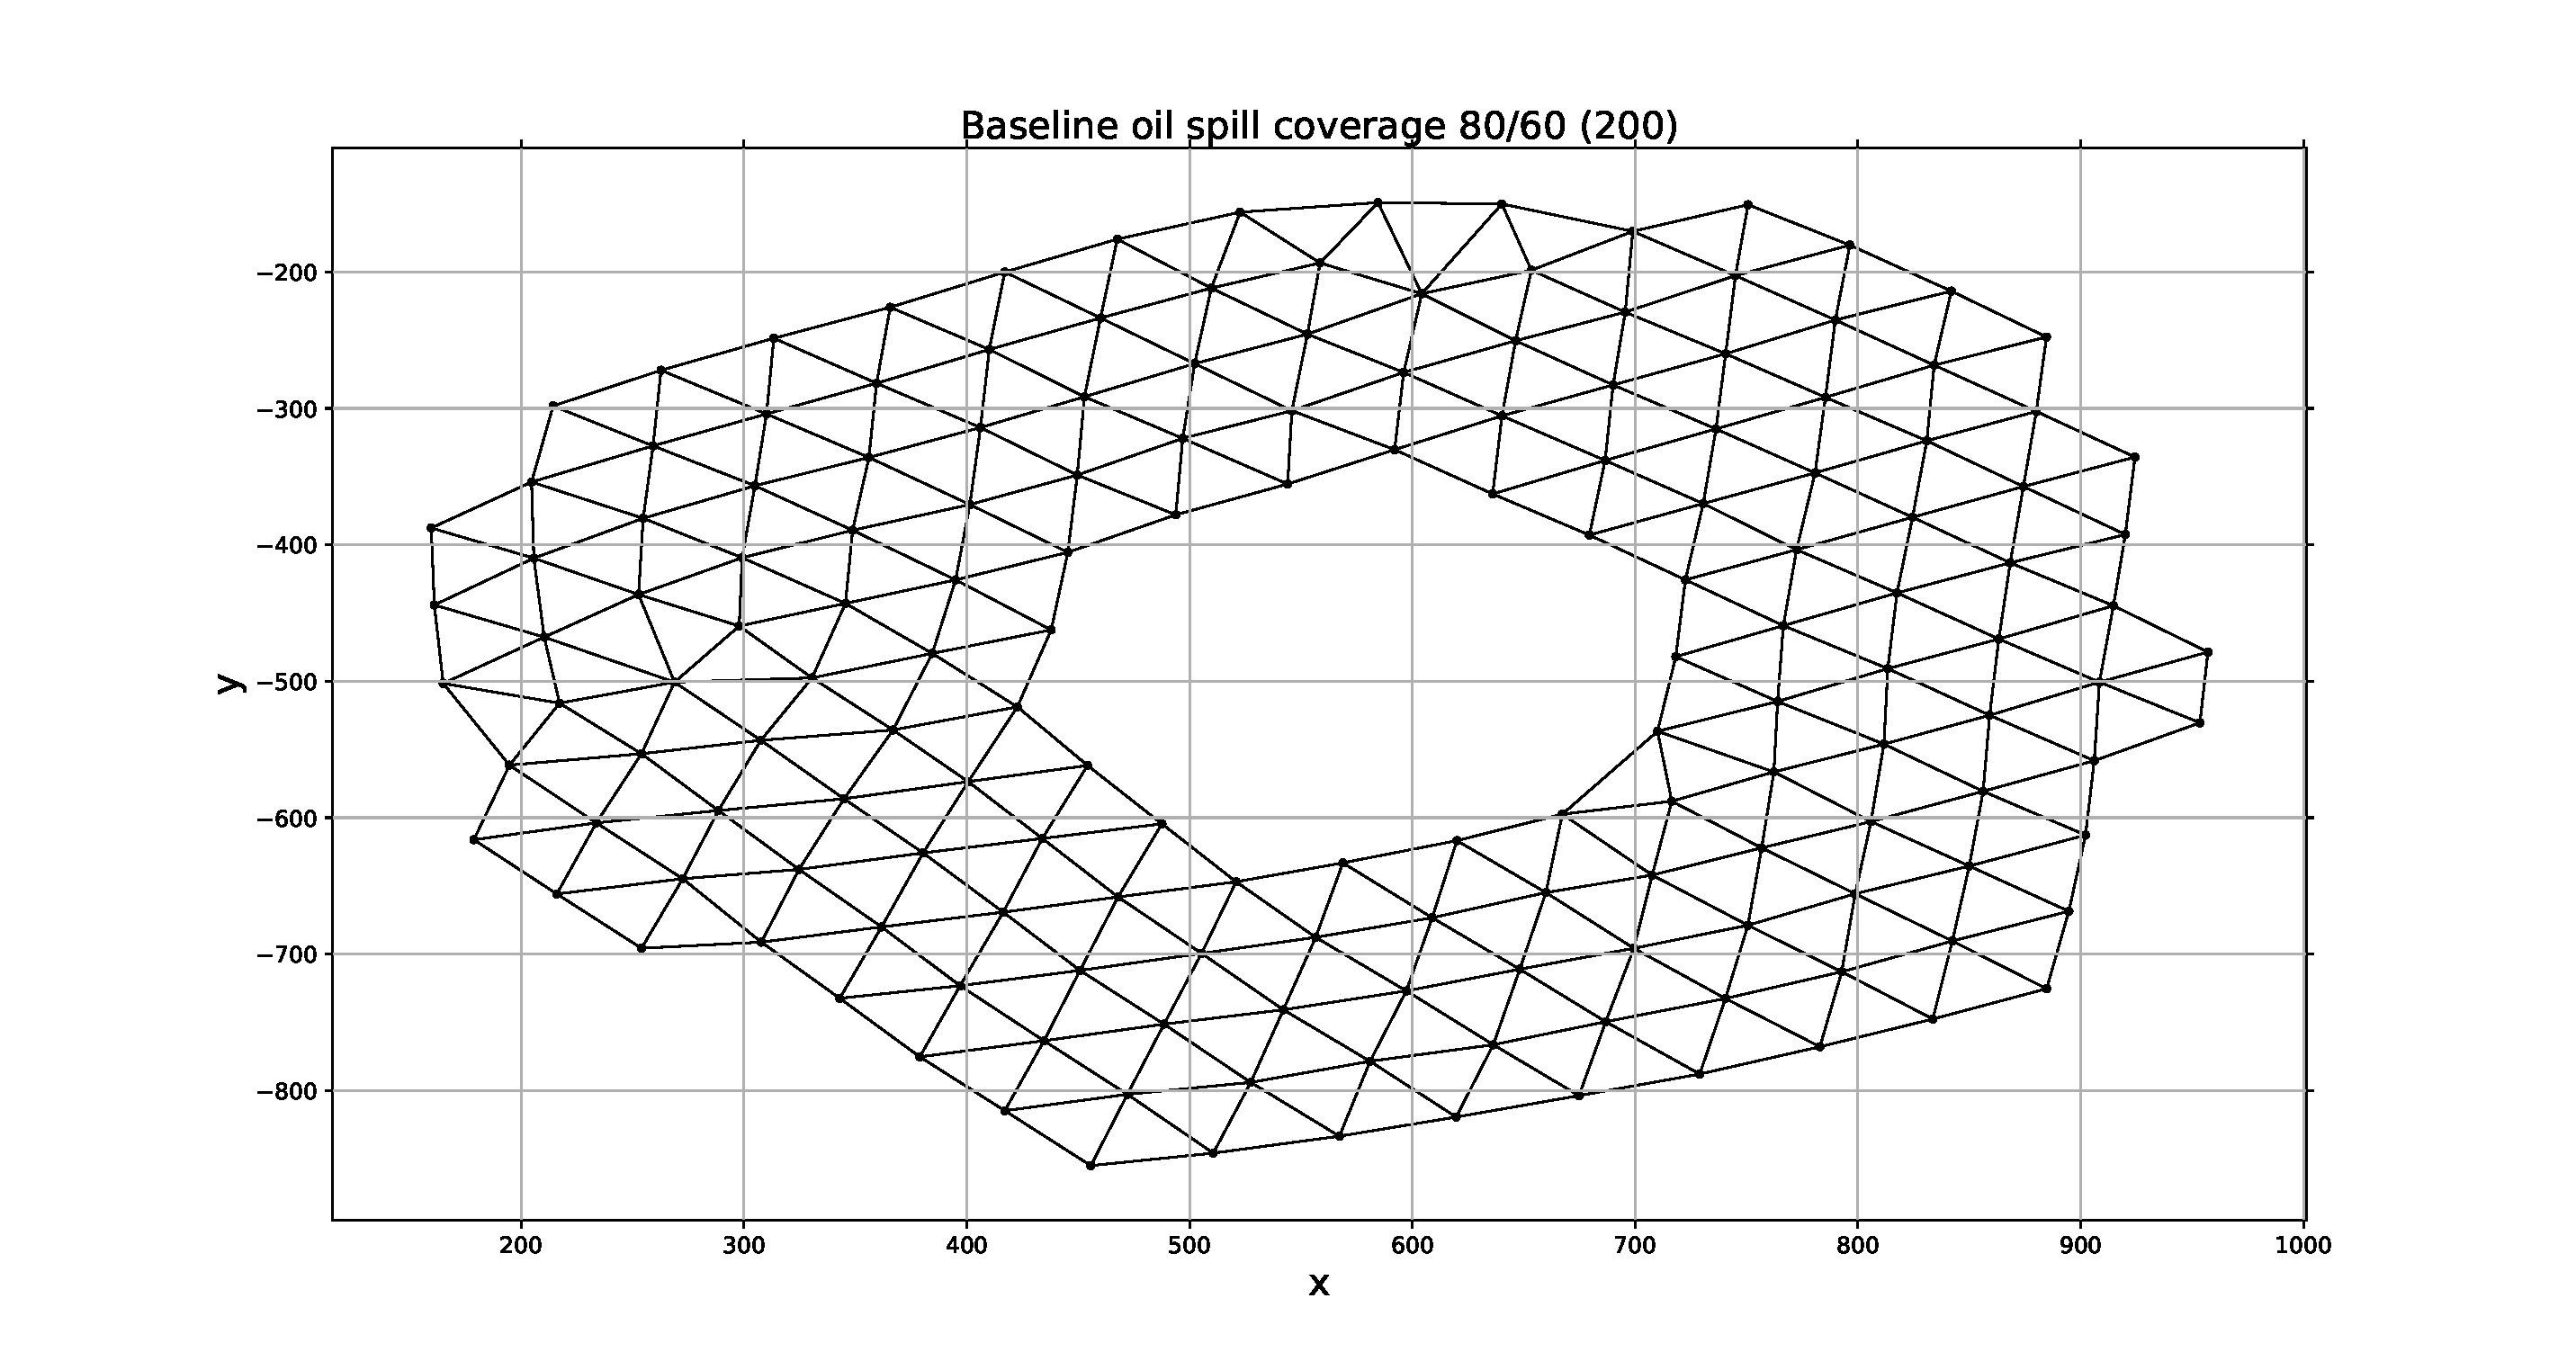
\includegraphics[width=5cm]{figures/OilSpillBase3}
%% \end{center}
%% \caption{End\label{concave:OilSpillBase3}}
%% \end{figure}

Figure~\ref{concave:OilSpillConcave1}, \ref{concave:OilSpillConcave2} and \ref{concave:OilSpillConcave3} shows the same simulation with void-reduction activated. The swarm expands as expected due to the field effects but in addition the concave reduction reduces the void within the swarm. This reduction in the void causes the swarm to shrink around the obstacle completely enclosing it at the obstacle perimeter. On the left hand side of~Fig.~\ref{concave:OilSpillConcave2} the percolation effect can be seen as described in~section~\ref{sec:ApplicationConcavePerimeters}.

%COVERBASELINE8060OILSPILLCONCAVE1.py 
\Figure[t!](topskip=0pt, botskip=0pt, midskip=0pt)[width=8.3cm]{figures/OilSpillConcave1}{Initial\label{concave:OilSpillConcave1}}
%% \begin{figure}
%% \begin{center}
%% 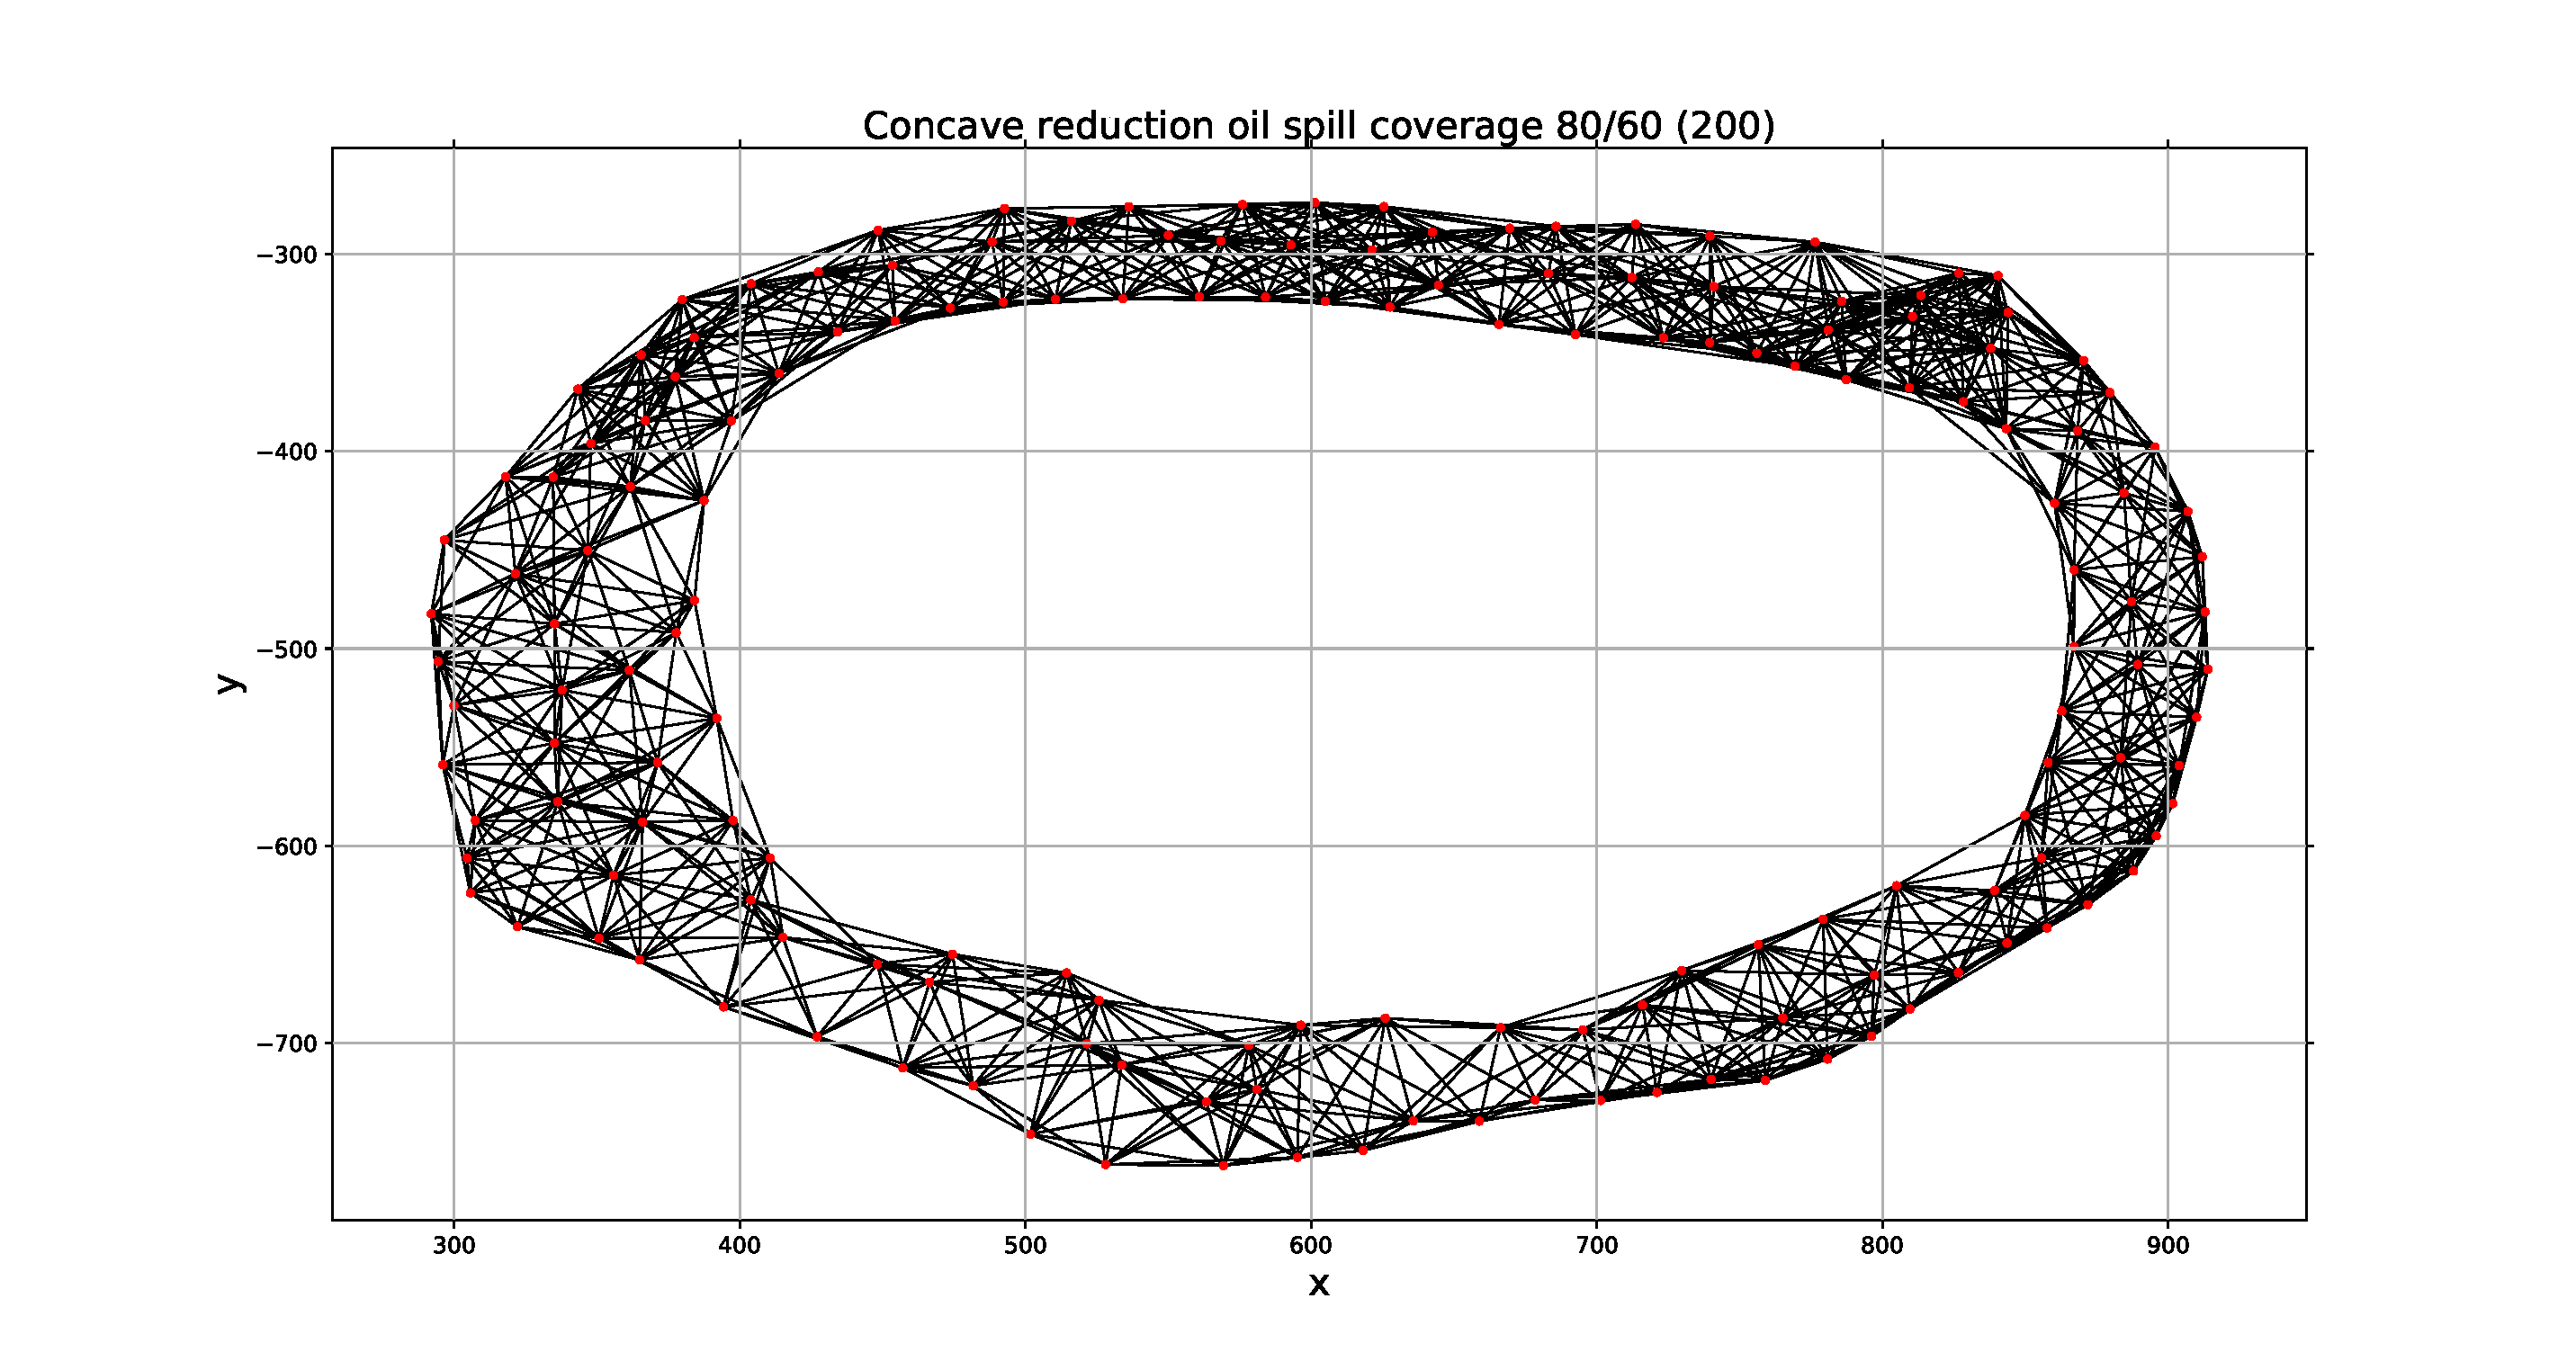
\includegraphics[width=5cm]{figures/OilSpillConcave1}
%% \end{center}
%% \caption{Initial\label{concave:OilSpillConcave1}}
%% \end{figure}

%COVERBASELINE8060OILSPILLCONCAVE2.py 
\Figure[t!](topskip=0pt, botskip=0pt, midskip=0pt)[width=8.3cm]{figures/OilSpillConcave2}{Partial\label{concave:OilSpillConcave2}}
%% \begin{figure}
%% \begin{center}
%% 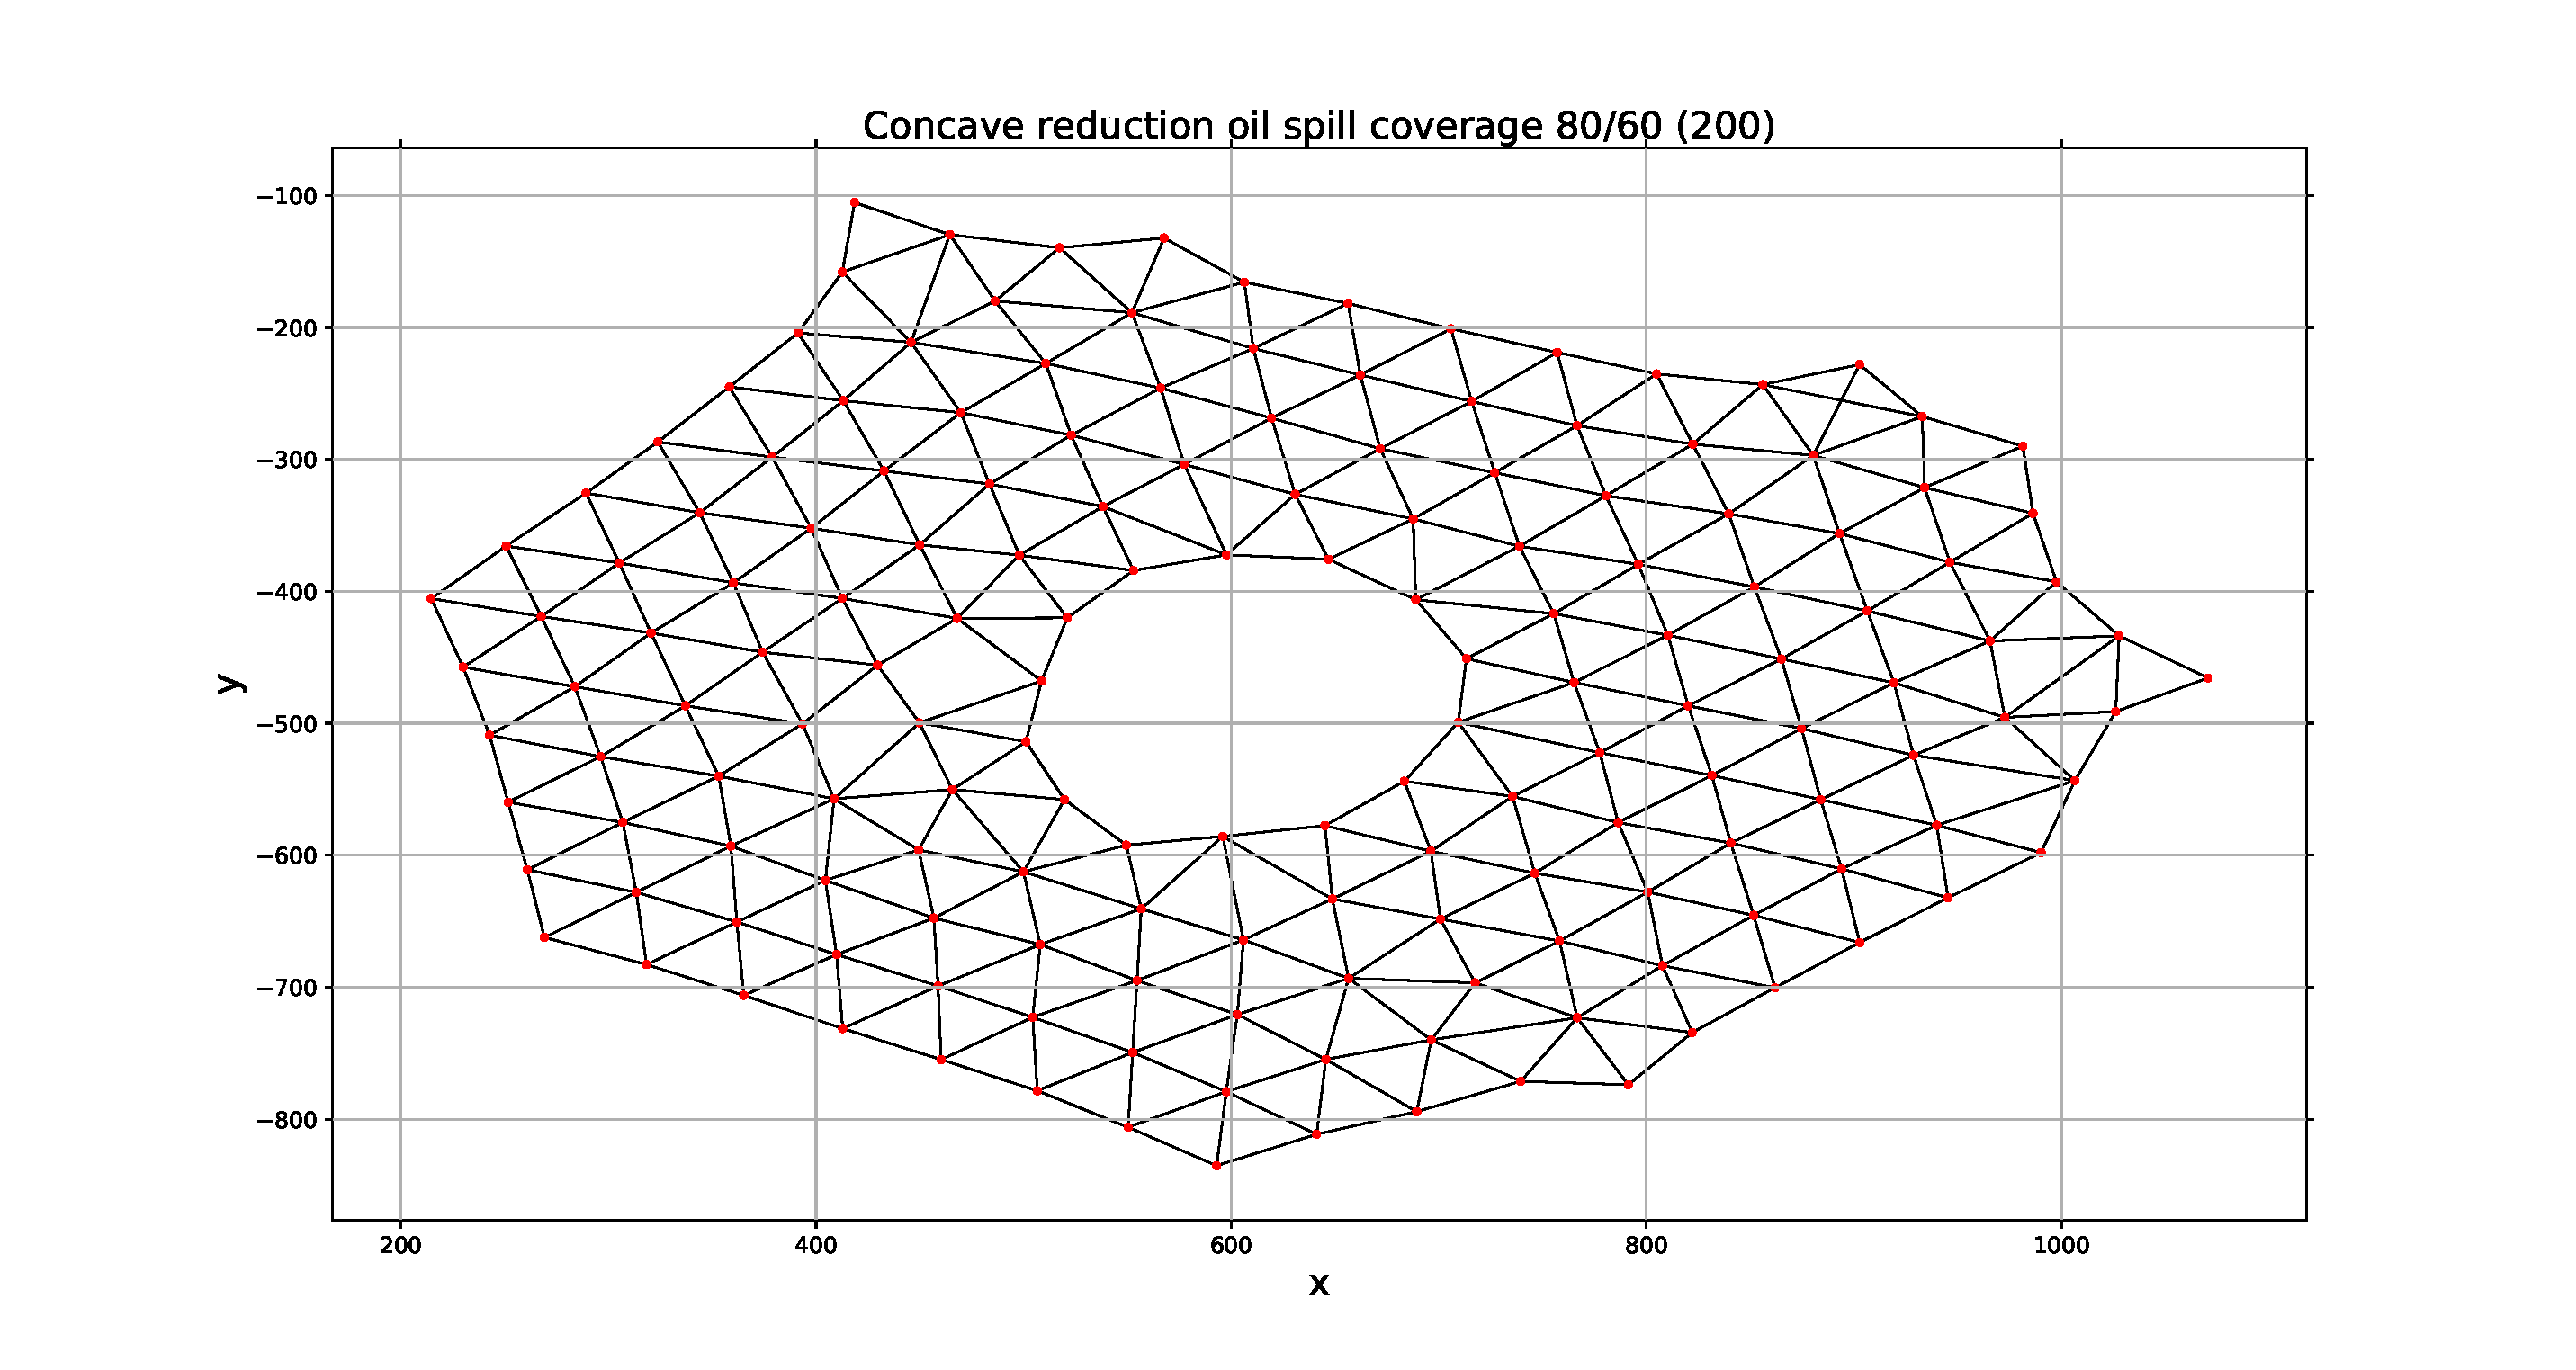
\includegraphics[width=5cm]{figures/OilSpillConcave2}
%% \end{center}
%% \caption{Partial\label{concave:OilSpillConcave2}}
%% \end{figure}

%COVERBASELINE8060OILSPILLCONCAVE3.py 
\Figure[t!](topskip=0pt, botskip=0pt, midskip=0pt)[width=8.3cm]{figures/OilSpillConcave3}{End\label{concave:OilSpillConcave3}}
%% \begin{figure}
%% \begin{center}
%% 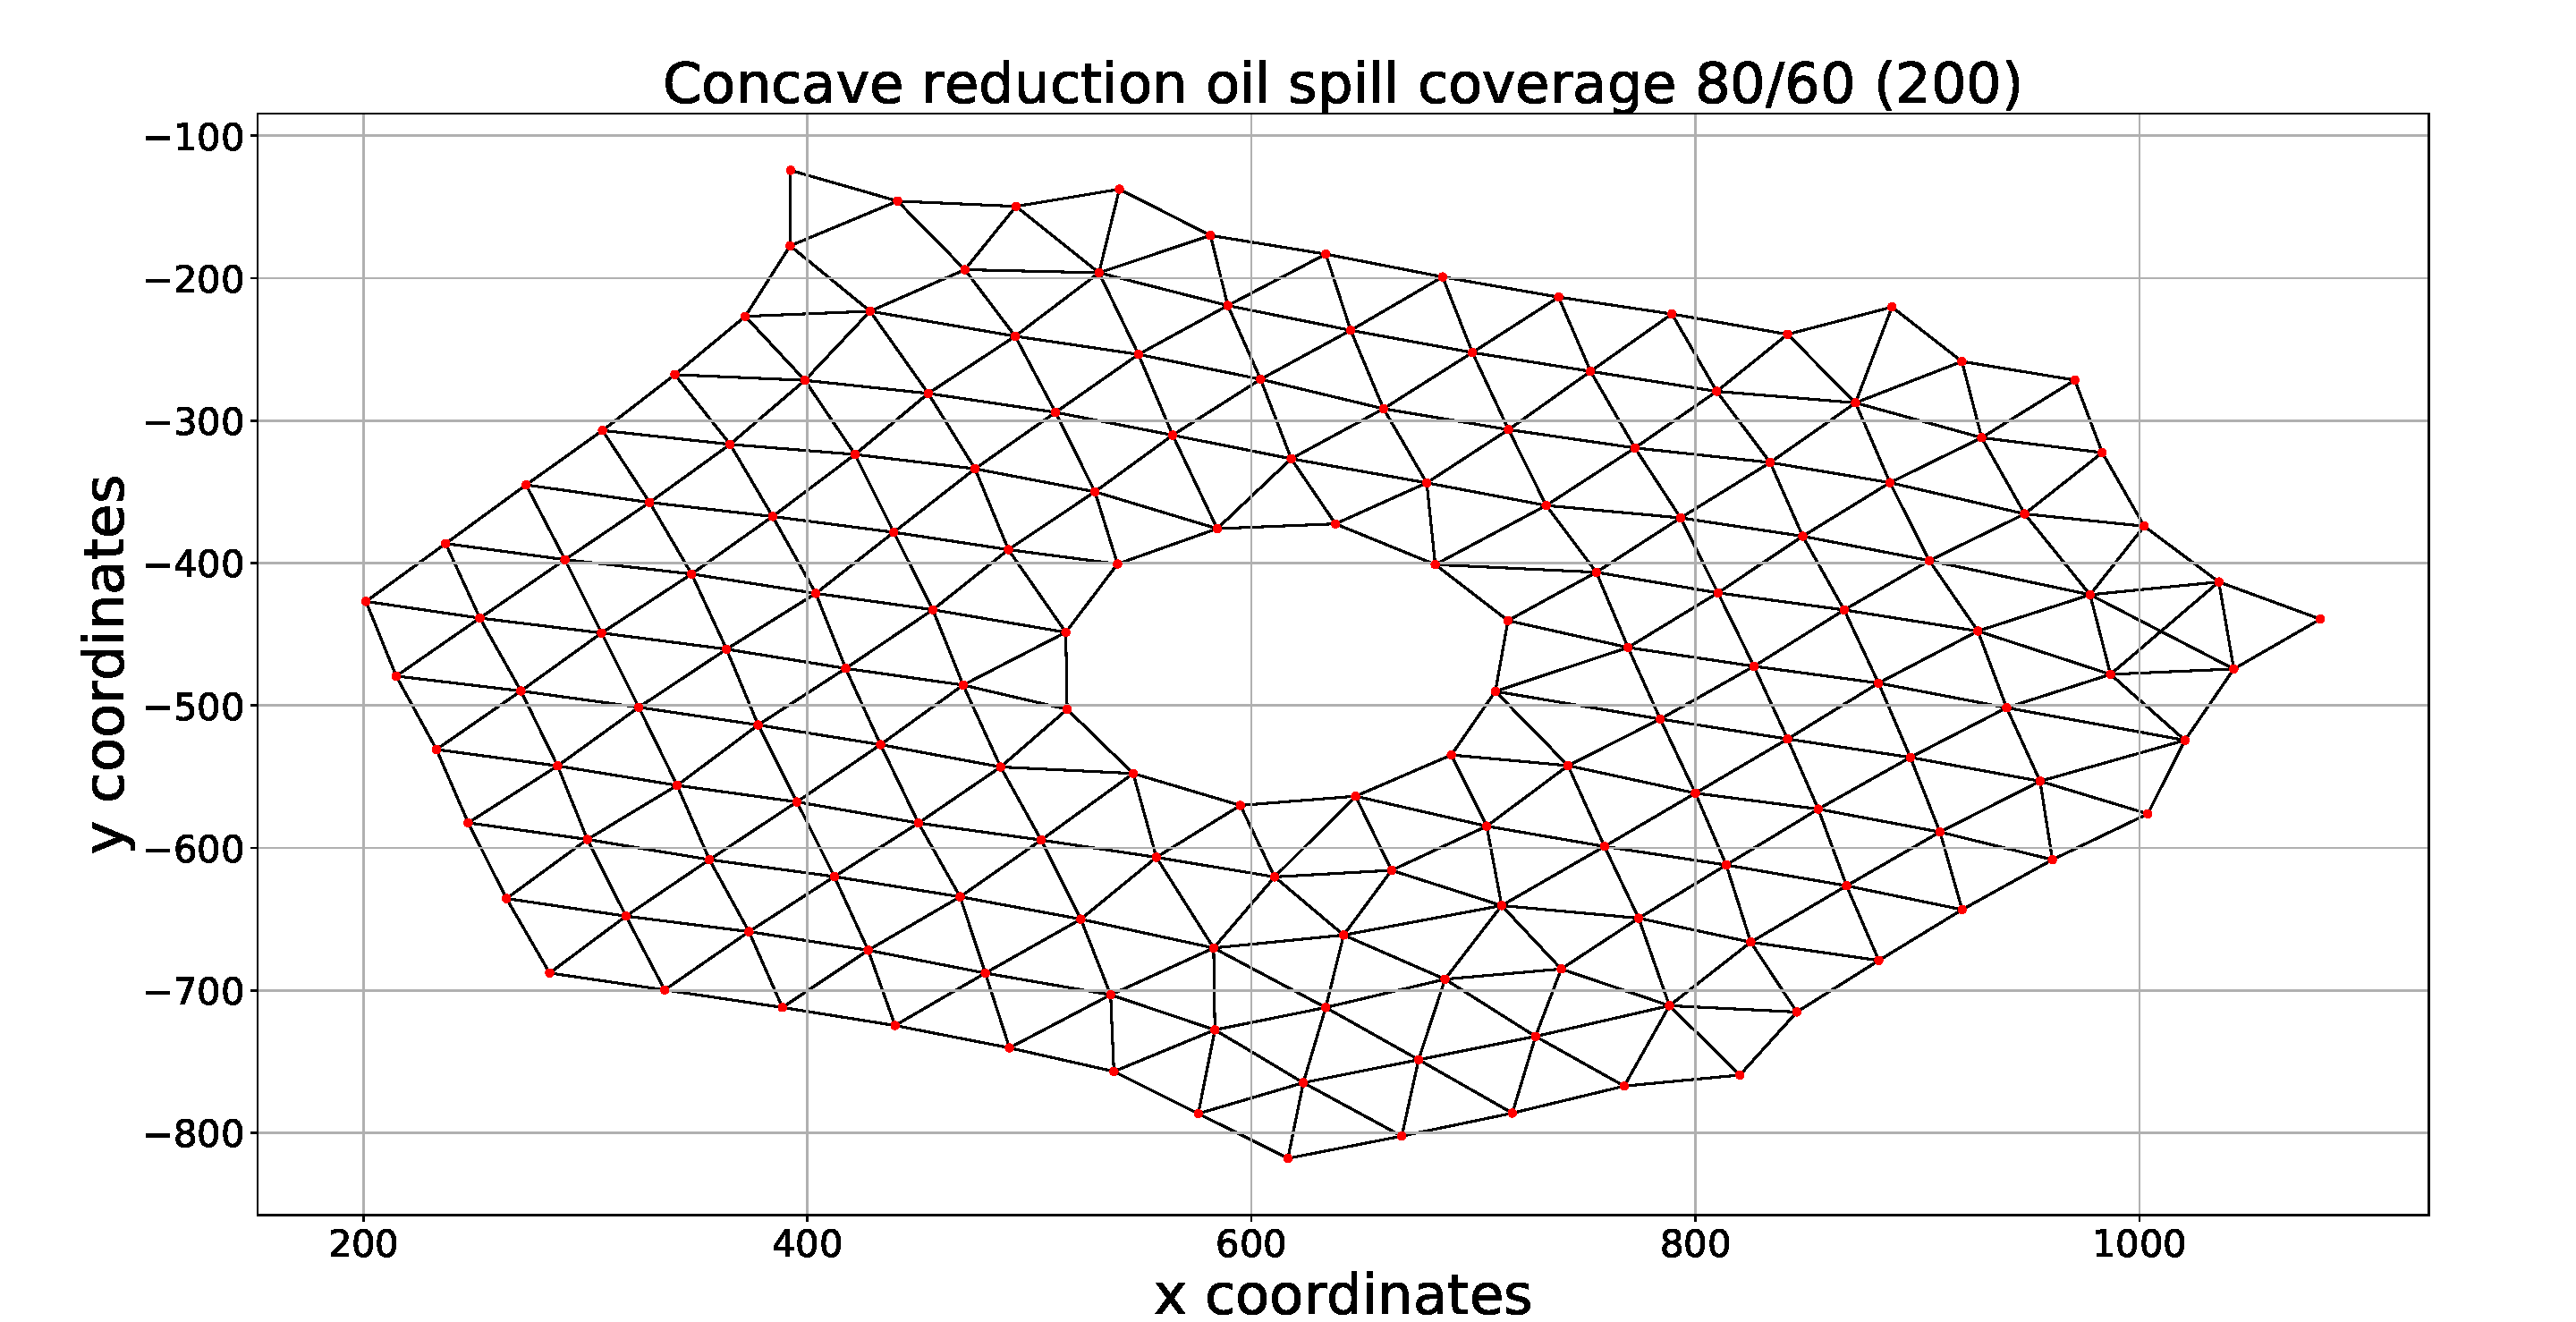
\includegraphics[width=5cm]{figures/OilSpillConcave3}
%% \end{center}
%% \caption{End\label{concave:OilSpillConcave3}}
%% \end{figure}
Figure~\ref{concave:OilSpillPerimeter8060-DIST-1} and \ref{concave:OilSpillPerimeter8060-MAG-1} show the effect of the concave reduction on the swarm's agent distribution compared to the baseline for the oil spillage scenario. 
Figure~\ref{concave:OilSpillPerimeter8060-DIST-1} shows distance distribution of the swarm for both the baseline (grey/black) and the concave reduction (red). The baseline expands then settles at approximately 6 seconds. This is also the case for the the concave reduction swarm. The baseline swarm, following the initial expansion, remains relatively slow changing with respect to distance and magnitude. The concave reduction swarm is affected more significantly, at approximately 10 seconds into the simulation the swarm's internal void perimeter makes contact with the oil spillage (obstacle). This has the effect of disrupting the average distance and average \textit{inter-agent magnitudes}. This effect diminishes slightly at approximately 18 seconds where the swarm's \textit{concave reduction vectors} cause the swarm to surround the spillage. The surrounding is followed by a few remaining changes caused by the agents at the spillage perimeter `snapping', the surrounding process is complete.
%BASELINE-CONCAVE-OIL-DIST.py
\Figure[t!](topskip=0pt, botskip=0pt, midskip=0pt)[width=8.3cm]{figures/OilSpillPerimeter8060-DIST-1}{Oil spill containment distance\label{concave:OilSpillPerimeter8060-DIST-1}}
%% \begin{figure}
%% \begin{center}
%% 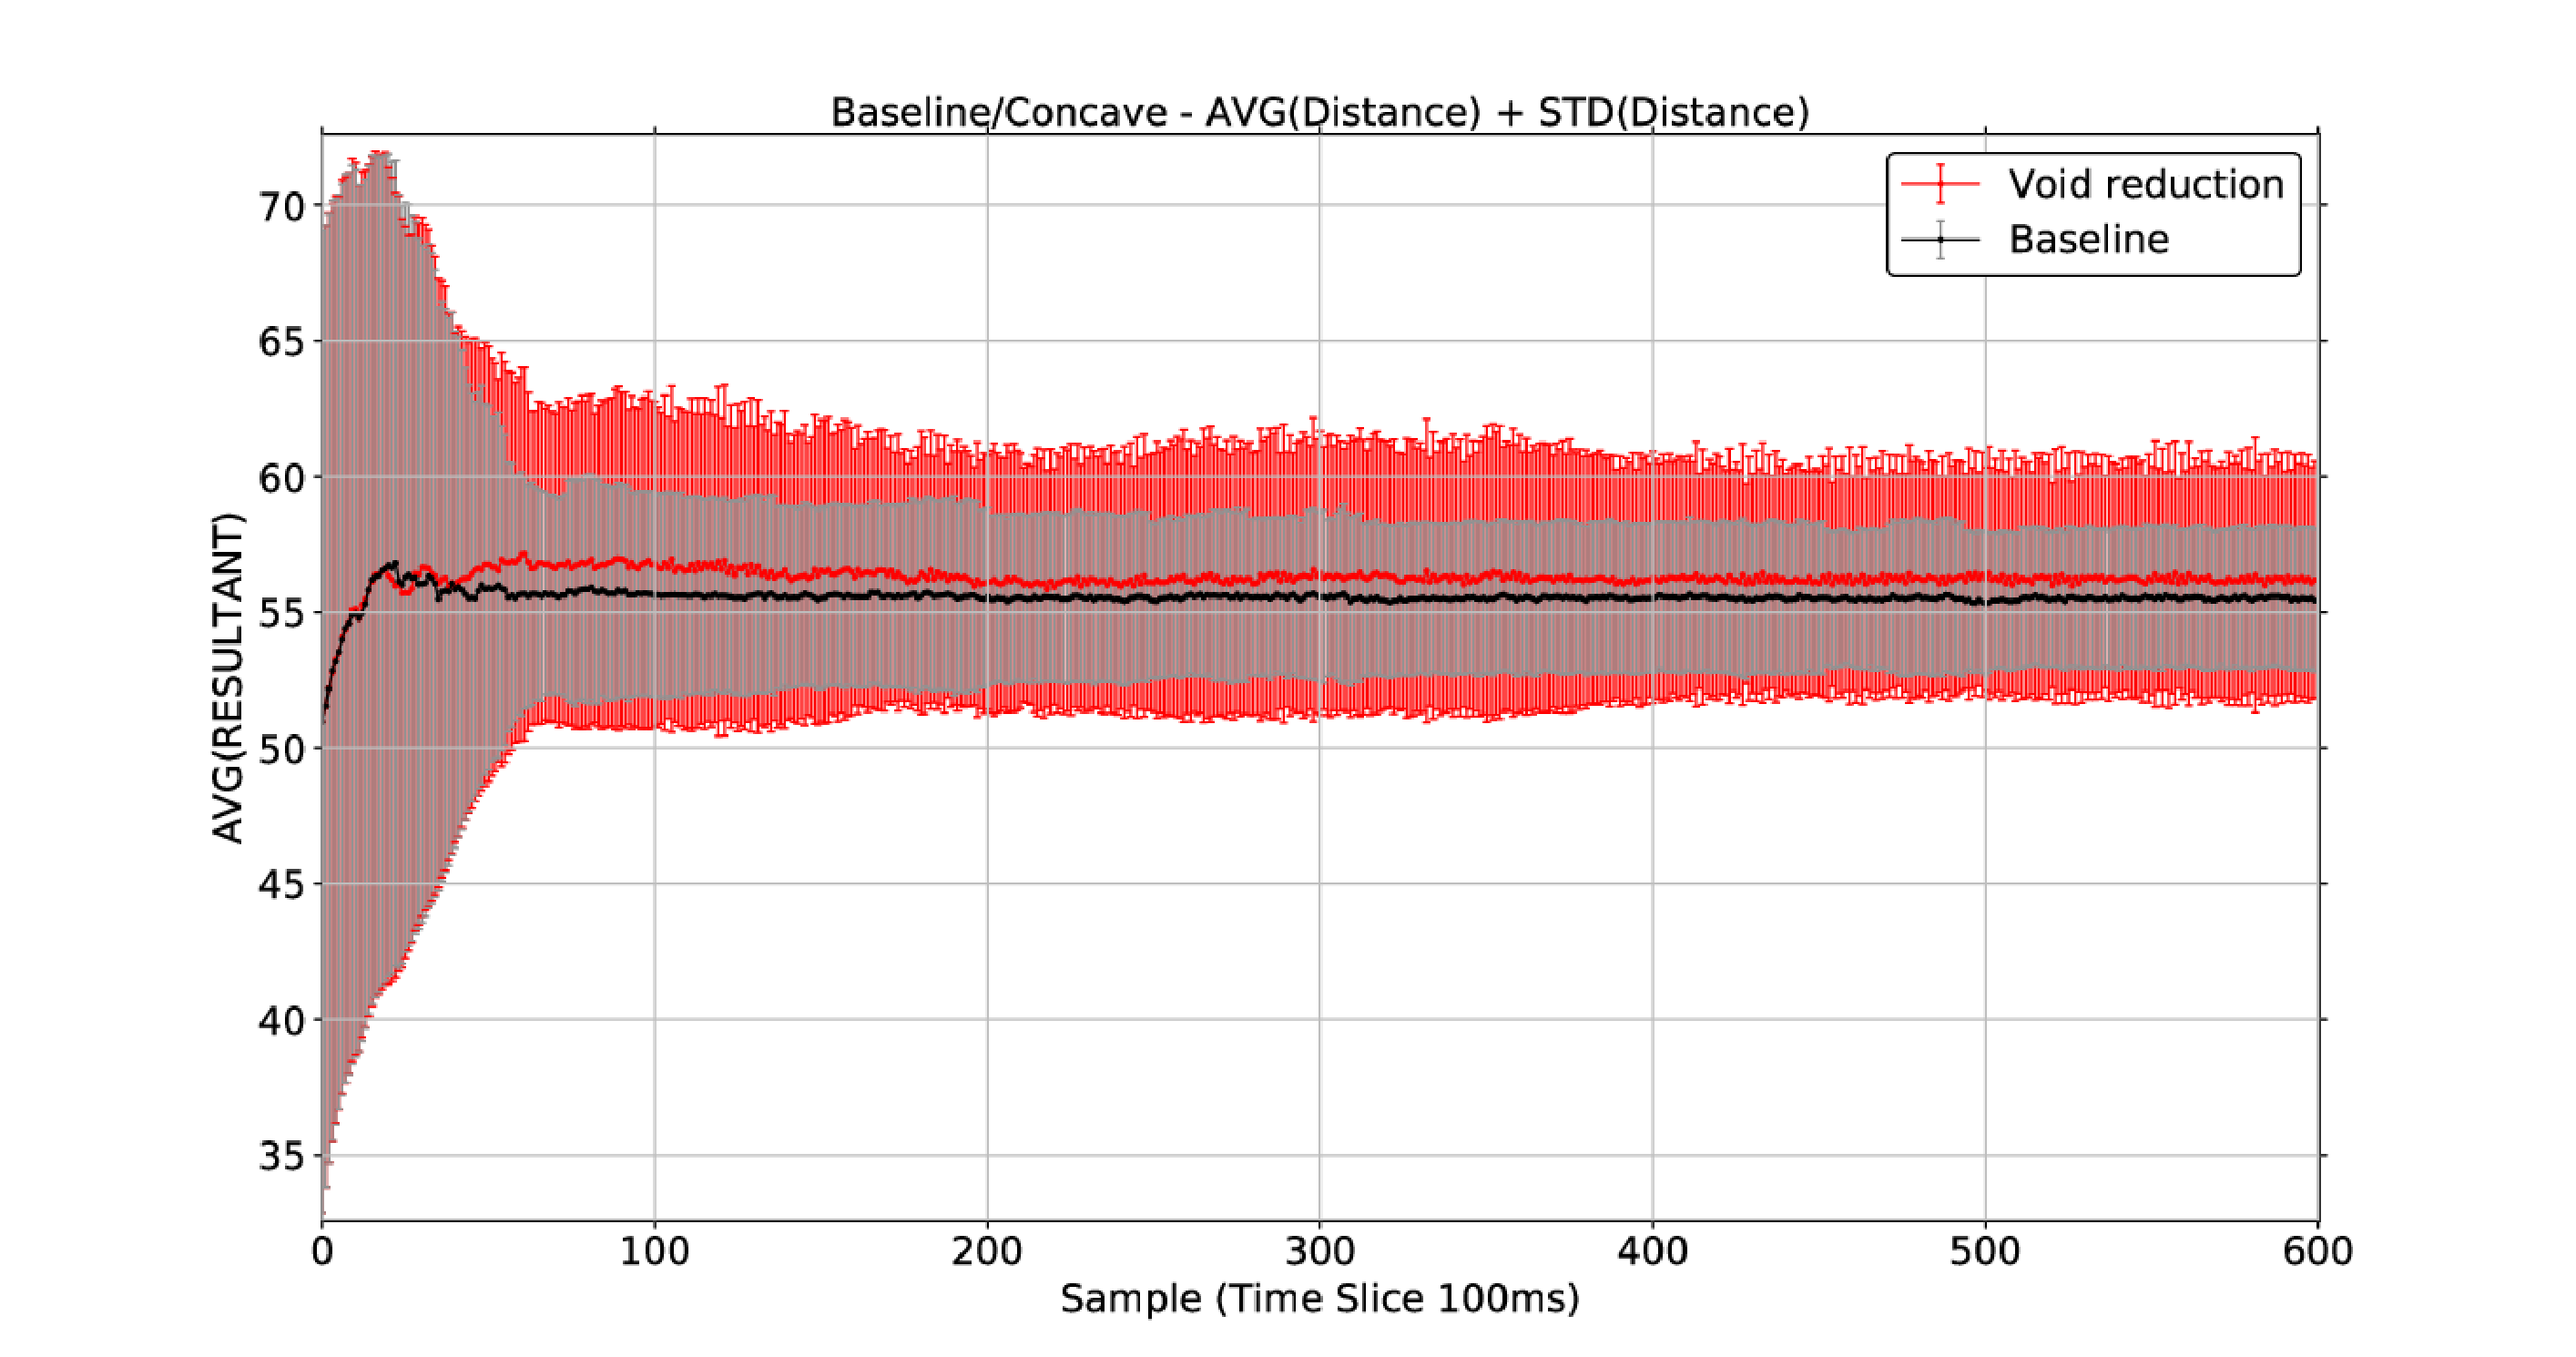
\includegraphics[width=8cm]{figures/OilSpillPerimeter8060-DIST-1}
%% \end{center}
%% \caption{Oil spill containment distance\label{concave:OilSpillPerimeter8060-DIST-1}}
%% \end{figure}
Figure~\ref{concave:OilSpillPerimeter8060-MAG-1} shows the comparison of the \textit{inter-agent magnitudes} for the baseline and concave reduction swarms. The initial deployment of the swarm is so condensed that the average \textit{inter-agent magnitude} is negative which indicates a high level of expansion. Within 2 seconds the expansion has reached a point where the average magnitude is positive which indicates the swarm is cohesive and will therefore remain as a single entity and be capable of surrounding an object without breaking apart.
%BASELINE-CONCAVE-OIL-MAG.py
\Figure[t!](topskip=0pt, botskip=0pt, midskip=0pt)[width=8.3cm]{figures/OilSpillPerimeter8060-MAG-1}{Oil spill containment magnitude\label{concave:OilSpillPerimeter8060-MAG-1}}
%% \begin{figure}
%% \begin{center}
%% 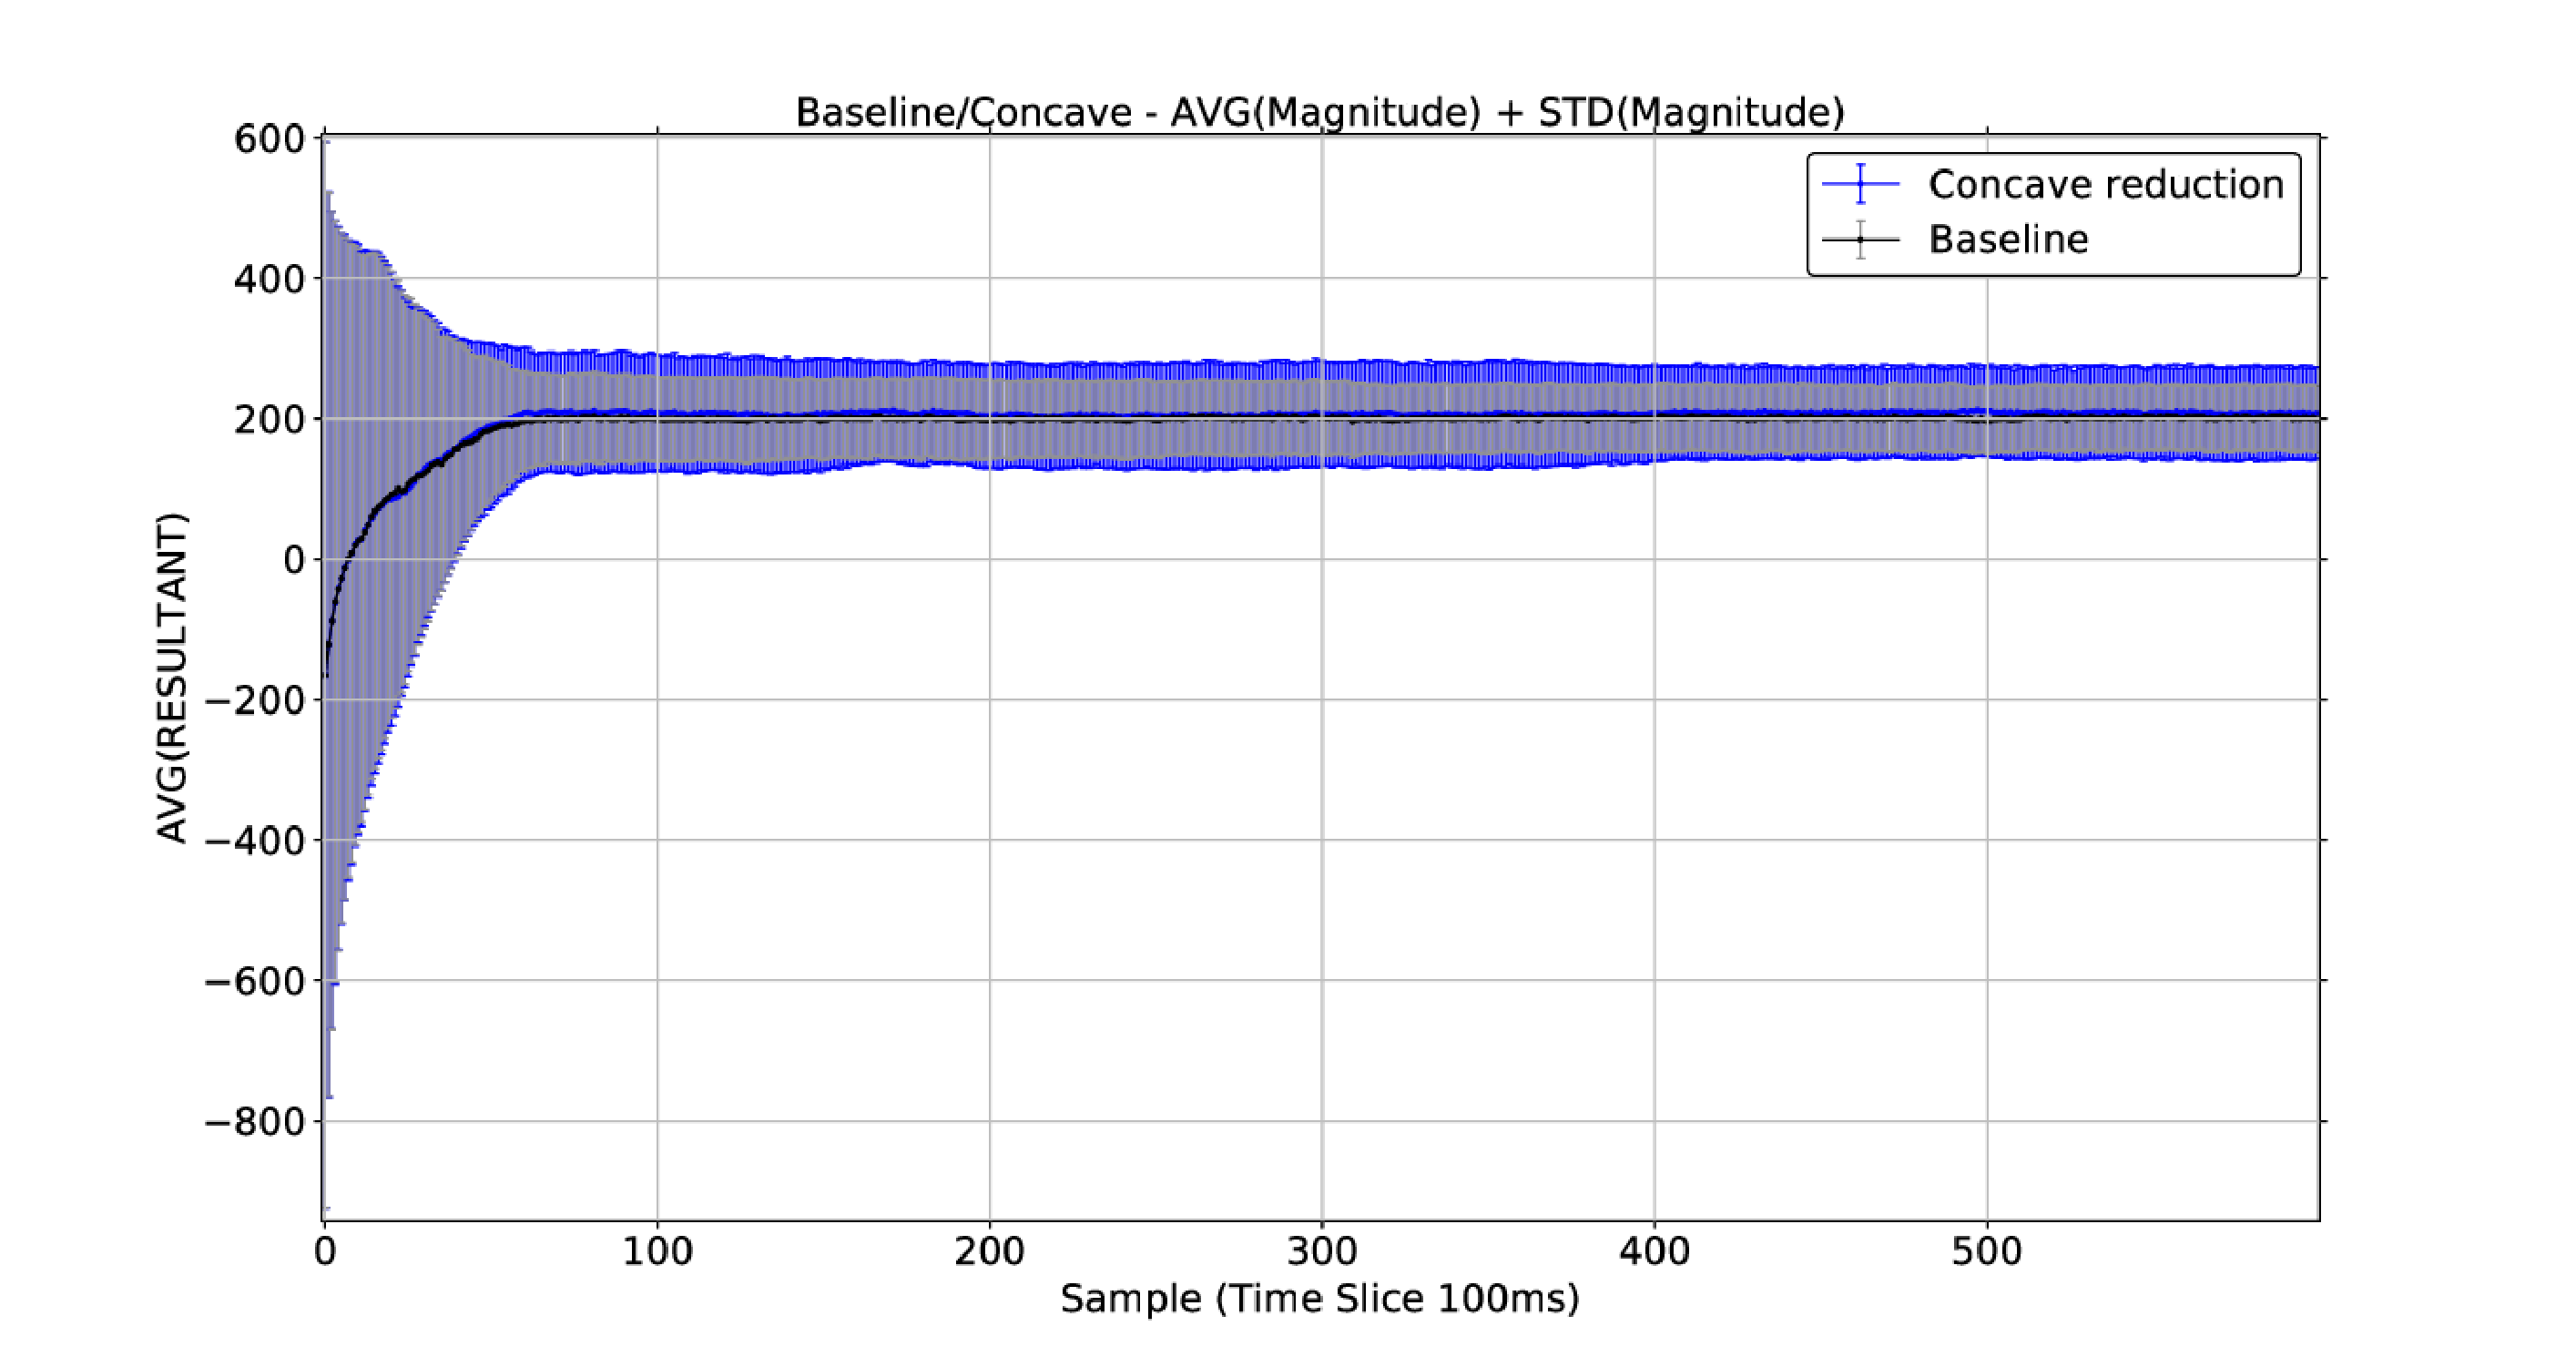
\includegraphics[width=8cm]{figures/OilSpillPerimeter8060-MAG-1}
%% \end{center}
%% \caption{Oil spill containment magnitude\label{concave:OilSpillPerimeter8060-MAG-1}}
%% \end{figure}
When the swarm `shrinks' to surround the obstacle there is an erratic change in the number of perimeter agents. Figure~\ref{concave:OilSpillPerimeter8060-1} shows the number of perimeter agents identified over the duration of the simulation. The graph shows the baseline swarm perimeter size decreases steadily and then settles (The swarm has not enclosed the spillage). The perimeter count has settled but as shown in Fig.~\ref{concave:OilSpillPerimeter8060-DIST-1} and \ref{concave:OilSpillPerimeter8060-MAG-1} the agents are still moving (magnitude variance and magnitude \textgreater 0) but the movement does not effect the overall structure. 
In the case of the concave reduction swarm the perimeter size is erratic due to the snapping effect~(Fig.~\ref{fig:OuterPerimeterJitter1} and \ref{fig:OuterPerimeterJitter2}). When the swarm encounters the obstacle at approximately 10 seconds there is a change due to `snapping' as the agents `fold' around the obstacle. The perimeter size then continues to fall gradually as the void is percolated out of the system, the perimeter size then stabilises as the obstacle is fully surrounded.

%PERIMETEROILSPILL.py
\Figure[t!](topskip=0pt, botskip=0pt, midskip=0pt)[width=8.3cm]{figures/OilSpillPerimeter8060-1}{Swarm perimeter size comparison\label{concave:OilSpillPerimeter8060-1}}
%% \begin{figure}
%% \begin{center}
%% 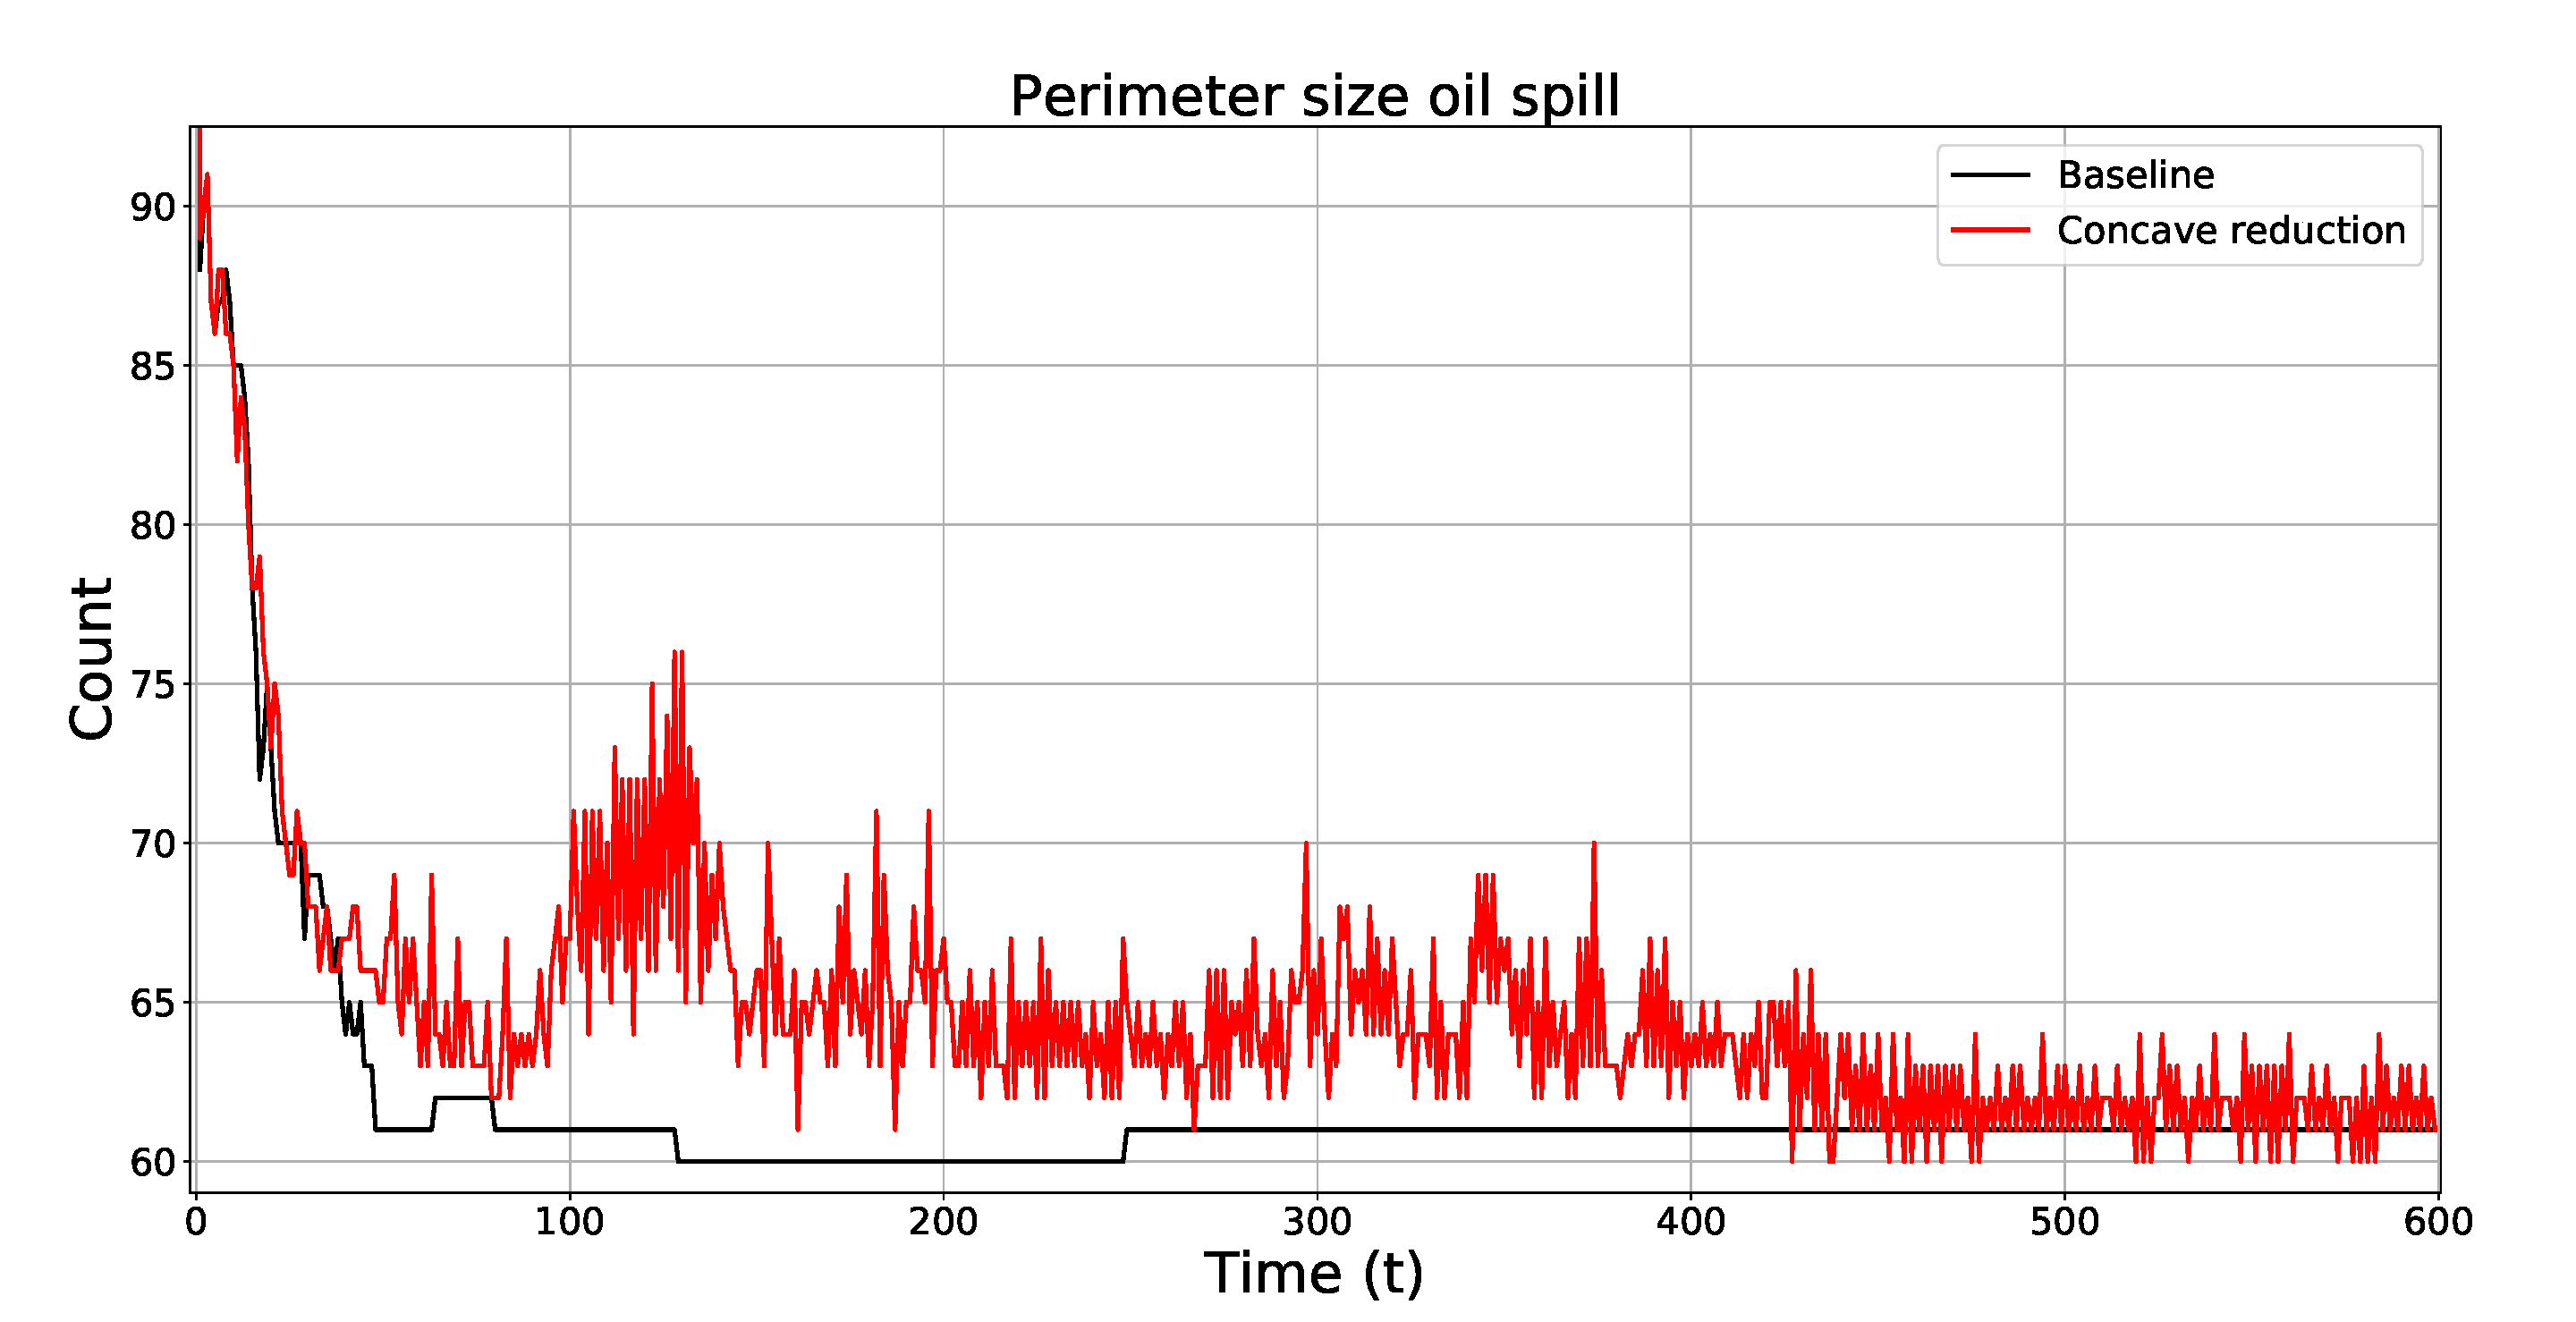
\includegraphics[width=8cm]{figures/OilSpillPerimeter8060-1}
%% \end{center}
%% \caption{Swarm perimeter size comparison\label{concave:OilSpillPerimeter8060-1}}
%% \end{figure}

\section{Concave reduction for destination-based swarms}\label{concave:mobileSwarm1}
A goal based swarm that is travelling between two points can have its path disrupted by an obstacle. This event can cause a swarm to develop an anomaly in the form of a void~(Fig.~\ref{concave:PerimeterObject2}) due to agents temporarily separating as the swarm passes the obstacle or the swarm may split entirely if the obstacle is very large~(Fig.~\ref{concave:PerimeterObject1}). 
When the object is small the cohesion and repulsion fields may make the swarm naturally reform~(Fig.~\ref{concave:PerimeterObject2}), however as the swarm progresses past the obstacle a void is created at the forward edge of the obstacle. If the purpose of the swarm is to deploy fertilizer over crops or carry out a reconnaissance task then the required full area coverage is not achieved. This failure to achieve total coverage reduces the effectiveness of employing a swarm to carry out tasks of this type.

\Figure[t!](topskip=0pt, botskip=0pt, midskip=0pt)[width=7cm]{figures/PerimeterObject2}{Swarm distortion via an object creating a void\label{concave:PerimeterObject2}}
%% \begin{figure}
%% \begin{center}
%% \includegraphics[width=5cm]{figures/PerimeterObject2}
%% \end{center}
%% \caption{Swarm distortion via an object creating a void\label{concave:PerimeterObject2}}
%% \end{figure}
\Figure[t!](topskip=0pt, botskip=0pt, midskip=0pt)[width=5cm]{figures/PerimeterObject1}{Swarm distortion via a large object\label{concave:PerimeterObject1}}
%% \begin{figure}
%% \begin{center}
%% \includegraphics[width=5cm]{figures/PerimeterObject1}
%% \end{center}
%% \caption{Swarm distortion via a large object\label{concave:PerimeterObject1}}
%% \end{figure}
Concave reduction has been shown to remove voids in static swarms in~section~\ref{sec:ApplicationConcavePerimeters}. Concave reduction can also be applied to a goal-based swarm to control coverage when passing small object: `small' means the maximum radius of the obstacle is of the order of the size of the neighbour field of an agent or less. When concave reduction is applied to the swarm it will surround the obstacle. Surrounding the obstacle creates a greater degree of coverage and increases the effectiveness of the swarm.
Taking the baseline swarm the swarm environment can be modified to include an obstacle in the path of the swarm. Figure~\ref{tab:SwarmCoverageParameters} shows the weightings and field effects for the baseline and concave reduction parameters for the experiment to demonstrate the concave reduction coverage improvement. Figure~\ref{voids:ObstacleTest1} shows the swarm and object setup within the simulator for the experiment.

\begin{table}
\caption{Swarm coverage parameters}
\label{tab:SwarmCoverageParameters}
\begin{center}
\begin{tabular}{| p{1.3cm} | p{1.3cm} | p{3.5cm} |}
\hline
\bf Weight \bf component & \bf Baseline \bf swarm & \bf Description \\ \hline
Sample rate & 100 & ms - Unit sampling interval\\  \hline
$k_{cr}$ & 100 & weight adjuster for concave vector\\  \hline
$k_o$ & 100 & weight adjuster for obstacle field\\  \hline
$k_c$ & 5 & weight adjuster for cohesion field\\  \hline
$k_r$ & 15 & weight adjuster for repulsion  field\\  \hline
$k_d$ & 35 & weight adjuster for destination vector\\  \hline
Repulsion Boundary & 45 & units\\  \hline
Neighbour Distance & 60 & units\\  \hline
Obstacle size & 60 & units\\  \hline
Speed & 20 & units/s\\  \hline
\end{tabular}
\end{center}
\end{table}

\Figure[t!](topskip=0pt, botskip=0pt, midskip=0pt)[width=8cm]{figures/ObstacleTest}{Initial configuration\label{voids:ObstacleTest1}}
%% \begin{figure}
%% \begin{center}
%% \includegraphics[width=8cm]{figures/ObstacleTest}
%% \end{center}
%% \caption{Initial configuration\label{voids:ObstacleTest1}}
%% \end{figure}

The experiment was run for 60 seconds to determine how the swarm is affected by the obstacle. The experiment is executed twice once with and once without concave reduction enabled. For Fig.~\ref{voids:ObstacleTest2} and \ref{voids:ObstacleTest3} the blue lines are generated by plotting the position of each agent as they progress towards the goal. Figure~\ref{voids:ObstacleTest2} is a path trace of the swarm as it propagates around the obstacle without concave reduction. The agents are repelled by the obstacle and the leading edge `flows' around the perimeter. Due to the compression caused by the agents passing around the obstacles an expansion is experienced at the trailing side and the agents are `pushed' such that the swarm reforms. However the time it takes for the compression to be removed causes the swarm to create a void at the forward side of the obstacle.  

%SWARMCOVER456060BASELINE.py
\Figure[t!](topskip=0pt, botskip=0pt, midskip=0pt)[width=8.3cm]{figures/SWARMCOVER456060BASELINE}{Swarm without concave reduction (60 Obstacle)\label{voids:ObstacleTest2}}
%% \begin{figure}
%% \begin{center}
%% \includegraphics[width=8cm]{figures/SWARMCOVER456060BASELINE}
%% \end{center}
%% \caption{Swarm without concave reduction (60 Obstacle)\label{voids:ObstacleTest2}}
%% \end{figure}
Figure~\ref{voids:ObstacleTest3} shows the path trace for the same environment settings with concave reduction enabled. In a similar way to the baseline experiment the leading edge agents approach the obstacle and through the repulsion effect of the obstacle the agents travel around the outer edge. Once the agents have passed the mid point of the obstacle the swarm splits in a similar way to the original experiment. The void is created in a similar way but when the split segments converge a change occurs. The meeting edges create a concave edge and the \textit{concave reduction vectors} affect the agents by `pulling' the `edges' together. This effect propagates back along the edges until the concave perimeter is reduced back to the obstacles forward edge. This effect slows the progress of the swarm's internal movement but closes the void. As the swarm progresses towards the destination the back portion of the swarm moves around the obstacle and swarm continues onto the destination.

%SWARMCOVER456060CONCAVE.py
\Figure[t!](topskip=0pt, botskip=0pt, midskip=0pt)[width=8.3cm]{figures/SWARMCOVER456060CONCAVE}{Swarm with concave reduction (60 Obstacle)\label{voids:ObstacleTest3}}
%% \begin{figure}
%% \begin{center}
%% \includegraphics[width=8cm]{figures/SWARMCOVER456060CONCAVE}
%% \end{center}
%% \caption{Swarm with concave reduction (60 Obstacle)\label{voids:ObstacleTest3}}
%% \end{figure}
\section{Conclusion}\label{voids:Conclusion}
This paper has demonstrated the concept of controlling a swarm's structure through the identification of perimeter anomalies in the form of concave edges. The identification of the anomalies is achieved locally by an individual agent without needing any communications infrastructure. The technique works with arbitrary sized swarms demonstrated here experimentally with a swarm of 200 agents.
Concave reduction is shown to work with static swarms such that a swarm can stablise to a more regular shape. It is possible for a swarm to develop where no concave reduction will be in operation which would allow the swarm to refer back to a baseline condition. Figure~\ref{voids:IdealSwarm} shows an ideal swarm shape that would result in no concave reduction based movement. 
\Figure[t!](topskip=0pt, botskip=0pt, midskip=0pt)[width=6cm]{figures/IdealSwarm}{Swarm structure with no concave reduction\label{voids:IdealSwarm}}
%% \begin{figure}
%% \begin{center}
%% \includegraphics[width=6cm]{figures/IdealSwarm}
%% \end{center}
%% \caption{Swarm structure with no concave reduction\label{voids:IdealSwarm}}
%% \end{figure}
This paper demonstrates by experiment that by altering the vector calculations for an agent based upon a set of stimuli it is possible to improve the coverage of an area and also create a `compression' effect that can increase the application landscape for swarming technologies that incorporate concave reduction.
%\clearpage
\bibliographystyle{plain}
\bibliography{thesis}
\newpage

\begin{IEEEbiography}[{\includegraphics[width=1in,height=1.25in,clip,keepaspectratio]{Images/eliot.pdf}}]{Neil Eliot}
has been a Senior Lecturer at Northumbria University since 1998.  Neil was awarded his Ph.D. from Northumbria in 2017, his Pg.C. in 1994, and his B.Sc. in 1989 all in Computing. His research areas include swarm theory and cybersecurity. Prior to this Neil worked in the chemical industry and the NHS. 
\end{IEEEbiography}

\begin{IEEEbiography}[{\includegraphics[width=1in,height=1.25in,clip,keepaspectratio]{Images/kenda.pdf}}]{David Kendall}
has been a Senior Lecturer in Computing at Northumbria University since 1989, except for a brief period as a Lecturer in Computer Science at Durham University (2001-02). Previously, he was a Research Associate at Newcastle University (1987-89), following experience as a Senior Software Engineer in industry (1983-86). He has an M.A. degree in Literae Humaniores from Oxford University, where he studied at New College. He received M.Sc. and Ph.D. degrees in Computing Science from Newcastle University. His research interests are in the area of formal modelling and analysis of embedded systems. 
\end{IEEEbiography}

\begin{IEEEbiography}[{\includegraphics[width=1in,height=1.25in,clip,keepaspectratio]{Images/moon.pdf}}]{Alun Moon} has been a Senior Lecturer in Computing at Northumbria Universiy since 2001. He has a PhD from Newcastle University in Electronic Engineering, a MSc from Hull University in Mechatronics, a PgDip in Astronomical Technology from Edinburgh University, and a BEng in Materials Science from Liverpool University.
	Prior experience as a research associate at Newcastle University included, embedded systems, engineering system modelling, and engineering visualisation.
\end{IEEEbiography}  
	
\begin{IEEEbiography}[{\includegraphics[width=1in,height=1.25in,clip,keepaspectratio]{Images/brock.pdf}}]{Michael Brockway}
has been a Senior Lecturer at Northumbria University for 17 years. His first degree is in pure and applied mathematics (1973-4), his Masters in mathematics (mathematical logic, category theory, 1975), and he has a PhD in computer science (formal methods for distributed embedded systems, 2010) from Northumbria University. Before that Michael worked in teaching and the computing industry.
\end{IEEEbiography}
  
\EOD
\end{document}
